\documentclass[12pt]{exam}

\newcommand{\Version}{11}
\newcommand{\Solutions}{1} 
\newcommand{\SetNumber}{0} % can set this variable to zero here it gets updated automatically later
\newcommand{\TwoPartPageTwo}{0} % some versions have two questions on teh second page


% LOAD PACKAGES
\usepackage{amsmath} % allows for align env and other things
\usepackage{amssymb} % 
\usepackage{mathtools} % allows for single apostrophe
\usepackage{enumitem} % allows for alpha lettering in enumerated lists
\usepackage{lastpage}
\usepackage{array} % for table alignments

% TIKZ DIAGRAMS (IF NEEDED)
\usepackage{color}
\usepackage{tikz}  \usetikzlibrary{arrows, automata} 
\usetikzlibrary{calc} 

% SUBSPACES AND ORTHOGONALITY
\newcommand{\Perp}{^{\perp}}
\newcommand{\Row}{\text{Row}}
\newcommand{\Col}{\text{Col}}
\newcommand{\Nul}{\text{Null}}
\newcommand{\Null}{\text{Null}}
\newcommand{\proj}{\text{proj}}
\newcommand{\Span}{\text{Span}}
\newcommand{\Rank}{\text{rank}}
\newcommand{\rank}{\text{rank}}
\newcommand{\Dim}{\text{dim}}

% ADJUST MARGINS
\usepackage[tmargin=2.0in,bmargin=1.75in]{geometry}
\geometry{margin=0.76in}

% COLORS FOR DIAGRAMS IN SOLUTIONS
\definecolor{DarkBlue}{rgb}{0.0,0.2,0.4} % 

% HEADERS AND FOOTERS
\pagestyle{headandfoot}
\runningfooter{}{}{}
\runningheader{\textit{\TestName}}{}{\textit{Page \thepage \ of \pageref{LastPage}} }
\headheight 42pt % distance from top of page to top of header
\headsep 12pt % space between header and top of body

\newcommand{\ID}{Fill in the blanks with a dark pen or pencil. 
Using only capital letters print your \\ first name: \framebox{\strut\hspace{4.2cm}}, last name: \framebox{\strut\hspace{4.2cm}}, the remaining digits \\[2pt] of your GTID:  \framebox{\strut $9$}\framebox{\strut $0$}\framebox{\strut\hspace{0.19cm}}\framebox{\strut\hspace{0.19cm}}\framebox{\strut\hspace{0.19cm}}\framebox{\strut\hspace{0.19cm}}\framebox{\strut\hspace{0.19cm}}\framebox{\strut\hspace{0.19cm}}\framebox{\strut\hspace{0.19cm}}, the High School you attend: \framebox{\strut\hspace{5.2cm}}.}

% ADJUST FIRST LINE IN PARAGRAPH INDENTATION 
\setlength\parindent{0pt}

% FONT FORMAT
\renewcommand*\rmdefault{lmss} % change font to lat mod ss


\begin{document}
    
% TEST SPECIFIC INFORMATION

\ifnum \Version=1 \newcommand{\TestName}{Year 1 MATH 1554 Final Exam Sample A} \fi % A FALL 2022 EXAM
\ifnum \Version=2 \newcommand{\TestName}{Year 1 MATH 1554 Final Exam Sample B} \fi % A FALL 2022 EXAM
\ifnum \Version=3 \newcommand{\TestName}{Year 1 MATH 1554 Final Exam Sample C} \fi % A FALL 2022 EXAM
\ifnum \Version=4 \newcommand{\TestName}{Year 1 MATH 1554 Final Exam Sample D} \fi % A FALL 2022 EXAM
\ifnum \Version=5 \newcommand{\TestName}{Year 1 MATH 1554 Final Exam Sample E} \fi % A FALL 2022 EXAM
\ifnum \Version=6 \newcommand{\TestName}{Year 1 MATH 1554 Final Exam Sample F} \fi % A FALL 2022 EXAM

\ifnum \Version=7 \newcommand{\TestName}{Year 1 Final Exam Version Dec 7 A1} \fi % A FALL 2023 EXAM
\ifnum \Version=8 \newcommand{\TestName}{Year 1 Final Exam Version Dec 7 A2} \fi % A FALL 2023 EXAM
\ifnum \Version=9 \newcommand{\TestName}{Year 1 Final Exam Version Dec 8 B1} \fi % A FALL 2023 EXAM
\ifnum \Version=10 \newcommand{\TestName}{Year 1 Final Exam Version Dec 8 B2} \fi % A FALL 2023 EXAM
\ifnum \Version=11 \newcommand{\TestName}{Year 1 Final Exam Version C1} \fi % A FALL 2023 EXAM
\ifnum \Version=12 \newcommand{\TestName}{Year 1 Final Exam Version C2} \fi % A FALL 2023 EXAM
\ifnum \Version=13 \newcommand{\TestName}{Year 1 Final Exam Version D1} \fi % A FALL 2023 EXAM
\ifnum \Version=14 \newcommand{\TestName}{Year 1 Final Exam Version D2} \fi % A FALL 2023 EXAM

% UPDATE SET NUMBER FOR ADDITIONAL RANDOMIZATION
\ifnum \Version=1 \renewcommand{\SetNumber}{1} \fi
\ifnum \Version=2 \renewcommand{\SetNumber}{2} \fi
\ifnum \Version=3 \renewcommand{\SetNumber}{1} \fi
\ifnum \Version=4 \renewcommand{\SetNumber}{2} \fi
\ifnum \Version=5 \renewcommand{\SetNumber}{1} \fi
\ifnum \Version=6 \renewcommand{\SetNumber}{2} \fi
\ifnum \Version=7 \renewcommand{\SetNumber}{1} \fi
\ifnum \Version=8 \renewcommand{\SetNumber}{1} \fi
\ifnum \Version=9 \renewcommand{\SetNumber}{1} \fi
\ifnum \Version=10 \renewcommand{\SetNumber}{1} \fi
\ifnum \Version=11 \renewcommand{\SetNumber}{1} \fi
\ifnum \Version=12 \renewcommand{\SetNumber}{1} \fi
\ifnum \Version=13 \renewcommand{\SetNumber}{1} \fi
\ifnum \Version=14 \renewcommand{\SetNumber}{1} \fi

% TITLE
\begin{center}
\ifnum \Solutions=1 {\Large {\color{DarkBlue}\textit{Solutions}}\\[6pt]}\fi
{\Large \TestName}
\end{center}

\textit{Work done on scratch paper will not be graded. You do not need to show your work on pages 1 and 2. }

\begin{questions}
\question[0.5] \ID

\ifnum \SetNumber = 1
    % UNIT 1 
    % INDEPENDENCE/SPAN/COMBINATIONS
    % TRANSFORMS

% UNIT 2
    % BASIS, RANK, INVERTIBILITY
    % SUBSPACES
    
% UNIT 3
    % DETERMINANTS OR EIG 1 EASY
    % DIAG AND INVERTIBILITY, OR DIAGONALIZABLE AND EIGENVALUES, OR OTHER DIAGONALIZABILITY THING

% UNIT 4
    % ORTHOG COMPLEMENTS
    % OTHER UNIT 4 THING
    
% UNIT 5
    % SVD
    % QUAD FORMS or SYMMETRIC MATRICES
    
\question[10] Indicate \textbf{true} if the statement is true, otherwise, indicate \textbf{false}.

\ifnum \SetNumber = 1
    \vspace{-0.8cm}
    \ifnum \Solutions = 0
        \setlength{\extrarowheight}{0.20cm}
    \fi
    \ifnum \Solutions = 1 
        \setlength{\extrarowheight}{0.00cm}
    \fi    
    \begin{center}
    \hspace{-.9cm}\begin{tabular}{ p{.15cm} p{14.2cm} p{.6cm} p{.6cm} }
        & & true &  false  \\[2pt] \hline 
        a) & \ifnum \Version=1         
    If there are non-trivial solutions to the linear system $A\vec x = \vec 0$, the columns of $A$ must be linearly independent.
    \ifnum \Solutions=1 {\color{DarkBlue} \textit{Solution:  } False. There would need to be non-pivotal columns, which means that the columns are dependent. } \fi
\fi
\ifnum \Version=2      
    If a linear system is consistent, then the solution set of the system either contains a unique solution when there are no free variables, or infinitely many solutions when there is at least one free variable.         
    \ifnum \Solutions=1 {\color{DarkBlue} \textit{Solution:  } True.  } \fi
\fi    
\ifnum \Version=3  
    If there are non-trivial solutions to the linear system $A\vec x = \vec 0$, the columns of $A$ must be linearly dependent.
    \ifnum \Solutions=1 {\color{DarkBlue} \textit{Solution:  } True. Non-trivial solutions implies that there are free variables. Free variables implies that some columns are not pivotal, which implies that the columns are dependent. } \fi
\fi    
\ifnum \Version=4    
    If the linear system $Ax=b$ is inconsistent, then $b$ cannot be in the span of the columns of $A$.
    \ifnum \Solutions=1 {\color{DarkBlue} \textit{Solution:  } True. The product $Ax$ is a linear combination of the columns of $A$ weighted by the entries of $x$. So if $Ax=b$ is inconsistent, there is no $x$ so that $Ax=b$, which is another way of saying that there is no linear combination of the columns that produces $b$. The span is the set of all possible linear combinations. } \fi
\fi   
\ifnum \Version=5    
    If the columns of a $5\times4$ matrix are linearly dependent, then the first 3 columns of the matrix are also a linearly dependent set of vectors. 
    \ifnum \Solutions=1 {\color{DarkBlue} \textit{Solution:  } False. A counter-example would be \setlength{\extrarowheight}{0.00cm}$A=\begin{pmatrix} 1&0&0&0\\0&1&0&0\\0&0&1&0\\0&0&0&0\\0&0&0&0\end{pmatrix}$. } \fi
\fi    
\ifnum \Version=6      
    If $\vec x_1$ is a solution to the inhomogeneous system $A\vec x = \vec b$, then any vector in Span\{$\vec x_1$\} is also a solution to $A\vec x = \vec b$.
    \ifnum \Solutions=1 {\color{DarkBlue} \textit{Solution:  } False. A vector in the span of $\vec v_1$ is the zero vector and the zero vector is not necessarily a solution to the system. } \fi
\fi           
\ifnum \Version=7 
     If $ \vec x_1$ and $\vec x_2$ solve the inhomogenous system $A\vec x = \vec b$, then $\vec x_1 - \vec x_2$ solves $A \vec x = 0$. 
    \ifnum \Solutions=1 {\color{DarkBlue} \textit{Solution: True.} 
    This is due to linearity.} \fi
\fi     
\ifnum \Version=8
    If the linear system $Ax=b$ is consistent, then $b$ must be in the span of the columns of matrix $A$.
    \ifnum \Solutions=1 {\color{DarkBlue} \textit{Solution:  } True. The product $Ax$ is a linear combination of the columns of $A$ weighted by the entries of $x$. So if $Ax=b$ is consistent, there is an $x$ so that $Ax=b$, which is another way of saying that there is a linear combination of the columns that produces $b$. The span is the set of all possible linear combinations. } \fi
\fi     
\ifnum \Version=9
  The span of two linearly independent vectors $\{\vec v_1, \vec v_2\} $ in $\mathbb R^4$ 
  is equal to the span of $\{\vec v_1 + \vec v_2, \vec v_1 - \vec v_2 \}$
    \ifnum \Solutions=1 {\color{DarkBlue} \textit{Solution}: True. Let $S = \Span \{\vec v_1 , \vec v_2 \}$, $ x = \vec v_1 + \vec v_2$ and $y = \vec v_1 - \vec v_2$. Then $x$ and $y$ are in $S$, they are not multiples of each other so they must be independent. And $x, y$ will span $S$ because $\dim S = 2$ and they are independent and in $S$.  
    } \fi
\fi     
\ifnum \Version=10
    If $\{\vec x,\vec y,\vec z\}$ is a linearly dependent set of vectors, then the set $\{\vec x, \vec y\}$ is also linearly dependent.
    \ifnum \Solutions=1 {\color{DarkBlue} \textit{Solution}: False. A counterexample would be $$\vec x = \begin{pmatrix}1\\0\\0 \end{pmatrix}, \quad \vec y = \begin{pmatrix} 0\\1\\0 \end{pmatrix}, \quad \vec z = \begin{pmatrix} 1\\1\\0\end{pmatrix}$$
    } \fi
\fi     
\ifnum \Version=11
    The span of two linearly independent vectors $\{\vec v_1, \vec v_2\} $ in $\mathbb R^4$ is equal to the span of $\{\vec v_1 + \vec v_2, 2\vec v_1 +2\vec v_2 \}$.
    \ifnum \Solutions=1 {\color{DarkBlue} \textit{Solution:  } false. Because if $S = \{\vec v_1 , \vec v_2 \}$ then $\dim(S) = 2$. But if the second set is $U = \{\vec v_1 + \vec v_2, 2\vec v_1 +2\vec v_2 \}$ then $\dim U = 1$ because the two vectors in the set are dependent.  } \fi
\fi     
\ifnum \Version=12
   If there are at least two distinct solutions to $A\vec x = \vec b$, then the columns of $A$ are linearly dependent. 
    \ifnum \Solutions=1 {\color{DarkBlue} \textit{Solution: True. }  
    $\vec x_1 - \vec x_2$ is a non-trival solution to $A x=0$.} \fi
\fi     
\ifnum \Version=13
    The span of two linearly independent vectors $\{\vec v_1, \vec v_2\} $ in $\mathbb R^4$  is equal to the span of the set $\{\vec v_1 + \vec v_2, \vec v_1 - \vec v_2 \}$
    \ifnum \Solutions=1 {\color{DarkBlue} \textit{Solution: True.} 
    } \fi
\fi     
\ifnum \Version=14
    If $\vec x_1$ is a solution to the inhomogeneous system $A\vec x = \vec b$, then any vector in Span\{$\vec x_1$\} is also a solution to $A\vec x = \vec b$.
    \ifnum \Solutions=1 {\color{DarkBlue} \textit{Solution:  } False. A vector in the span of $\vec v_1$ is the zero vector and the zero vector is not necessarily a solution to the system. } \fi
\fi     
\ifnum \Version=15
     If $ \vec x_1$ and $\vec x_2$ solve the inhomogenous system $A\vec x = \vec b$, then $\vec x_1 + \vec x_2$ solves $A \vec x = \vec b$. 
    \ifnum \Solutions=1 {\color{DarkBlue} \textit{Solution: False.} 
    $A(\vec x_1 + \vec x_2)=2\vec b $, which is not $\vec b$, since $\vec b$ is not zero. } \fi
\fi     
\ifnum \Version=16
    TRUE FALSE ON LINEAR INDEPENDENCE OR SPAN OR LINEAR COMBINATIONS
    \ifnum \Solutions=1 {\color{DarkBlue} \textit{Solution: True. }  
    } \fi
\fi     
\ifnum \Version=17
    TRUE FALSE ON LINEAR INDEPENDENCE OR SPAN OR LINEAR COMBINATIONS
    \ifnum \Solutions=1 {\color{DarkBlue} \textit{Solution: True. }  
    } \fi
\fi     
\ifnum \Version=18
    TRUE FALSE ON LINEAR INDEPENDENCE OR SPAN OR LINEAR COMBINATIONS
    \ifnum \Solutions=1 {\color{DarkBlue} \textit{Solution: True. }  
    } \fi
\fi     
& $\bigcirc$  & $\bigcirc$ \\ 
        b) & % TRANSFORMS
\ifnum \Version=1         
    If $A$ is $2 \times 3$, then the transformation $\vec x \to A\vec x$ cannot be one-to-one.
    \ifnum \Solutions=1 {\color{DarkBlue} \textit{Solution:  } True. For the transform to be one-to-one every column of $A$ would need to be pivotal, which is impossible because there are more columns than rows.  } \fi
\fi
\ifnum \Version=2      
    If $A$ is $m\times n$, $\vec x \in \mathbb R^n$, and there are some vectors $\vec b \in \mathbb R^m$ that are not in the range of the transform $T(\vec x) = A\vec x$, then there cannot be a pivot in every row of $A$. 
    \ifnum \Solutions=1 {\color{DarkBlue} \textit{Solution:  } True. If there is a pivot in every row of $A$ then the corresponding linear system is always consistent.} \fi
\fi    
\ifnum \Version=3  
    If $A$ is $2 \times 3$, then the transformation $\vec x \to A\vec x$ cannot be onto. 
    \ifnum \Solutions=1 {\color{DarkBlue} \textit{Solution:  }  False. The transform is onto when there are pivots in every row of the standard matrix $A$, which is possible when $A$ is $2\times 3$. } \fi
\fi    
\ifnum \Version=4    
    If $A$ is the standard matrix for a linear transform that is one-to-one and onto, then $A$ must be square. 
    \ifnum \Solutions=1 {\color{DarkBlue} \textit{Solution:  } True. There needs to be pivots in every row and every column and that can only happen when $A$ is square.} \fi
\fi   
\ifnum \Version=5    
    If $A$ is $m\times n$, $\vec x \in \mathbb R^n$, and there are some vectors $\vec b \in \mathbb R^m$ that are not in the range of the transform $T(\vec x) = A\vec x$, then there cannot be a pivot in every column of $A$. 
    \ifnum \Solutions=1 {\color{DarkBlue} \textit{Solution:  } False. A counter-example: \setlength{\extrarowheight}{0.0cm}$A=\begin{pmatrix} 1&0\\0&1\\0&0\end{pmatrix}, b = \begin{pmatrix} 1\\1\\1\end{pmatrix}$. } \fi
\fi    
\ifnum \Version=6      
    If $A$ is $n\times n$ and for every $\vec b \in \mathbb R^n$ there is exactly one $\vec x \in \mathbb R^n$ so that $A \vec x = \vec b$, then $ T_A(\vec x) = A\vec x $ is one-to-one.
    \ifnum \Solutions=1 {\color{DarkBlue} \textit{Solution:  } True. This is the definition of one-to-one. } \fi
\fi        
\ifnum \Version=7 
    If $A$ is a $5 \times 3$ matrix, then the transformation $T (\vec x)=A\vec x$ is not onto. 
    \ifnum \Solutions=1 {\color{DarkBlue} \textit{Solution: True.} 
    The range is at most 3 dimensional in a 5 dimensional space.} \fi
\fi     
\ifnum \Version=8
     If the system $Ax=b$ is inconsistent, then the transform $T(\vec x) = A\vec x$ is not onto. 
    \ifnum \Solutions=1 {\color{DarkBlue} \textit{Solution: True.  } 
    You can't solve $A\vec x = b$. } \fi
\fi     
\ifnum \Version=9
    If the system $Ax=b$ is consistent for every choice of $b$ then the transform $T(\vec x) = A\vec x$ is not onto. 
    \ifnum \Solutions=1 {\color{DarkBlue} \textit{Solution: False.   } 
     You can solve $T \vec x =b$ for all $b$.}  \fi
\fi     
\ifnum \Version=10
    If $A$ is a $3 \times 5$ matrix, then the transformation $T (\vec x)=A\vec x$ is not one-to-one. 
    \ifnum \Solutions=1 {\color{DarkBlue} \textit{Solution: True.} 
    The columns of $A$ will be dependent, so there is a non-trivial solution to $T \vec x =0$.}\fi
\fi     
\ifnum \Version=11
 If $A$ is $4\times 6$, then the transformation $\vec x \to A\vec x$ cannot be onto. 
    \ifnum \Solutions=1 {\color{DarkBlue} \textit{Solution:  }  False. The transform is onto when there are pivots in every row of the standard matrix $A$, which is possible when $A$ is $2\times 3$. }  \fi
\fi     
\ifnum \Version=12
    If matrix $A$ has a pivot in every column, then the transformation $T (\vec x) = A\vec x$ is one-to-one.  
    \ifnum \Solutions=1 {\color{DarkBlue} \textit{Solution:  }  
    True. The columns are linearly independent.} \fi
\fi   
\ifnum \Version=13
    If $A$ is $m\times n$, $\vec x \in \mathbb R^n$, and there are some vectors $\vec b \in \mathbb R^m$ that are not in the range of the transform $T(\vec x) = A\vec x$, then there cannot be a pivot in every column of $A$. 
    \ifnum \Solutions=1 {\color{DarkBlue} \textit{Solution:  } False. A counter-example: \setlength{\extrarowheight}{0.0cm}$A=\begin{pmatrix} 1&0\\0&1\\0&0\end{pmatrix}, b = \begin{pmatrix} 1\\1\\1\end{pmatrix}$. } \fi
\fi   
\ifnum \Version=14
    If $A$ is $m\times n$ and for every $\vec b \in \mathbb R^m$ there is at least one $\vec x \in \mathbb R^n$ so that $A \vec x = \vec b$, then every column of $A$ must be pivotal. 
    \ifnum \Solutions=1 {\color{DarkBlue} \textit{Solution:  }  False. Every row would be pivotal.} \fi
\fi   
\ifnum \Version=15
    TRUE FALSE ON LINEAR TRANSFORMS
    \ifnum \Solutions=1 {\color{DarkBlue} \textit{Solution:  }  True. } \fi
\fi   
\ifnum \Version=16
    TRUE FALSE ON LINEAR TRANSFORMS
    \ifnum \Solutions=1 {\color{DarkBlue} \textit{Solution:  }  True. } \fi
\fi   
& $\bigcirc$  & $\bigcirc$ \\   

        c) & % BASIS, RANK, INVERTIBILITY
\ifnum \Version=1         
    If $A$ is $m\times n$, and $\Rank (A) = n$, then the columns of $A$ are linearly independent.
    \ifnum \Solutions=1 {\color{DarkBlue} \textit{Solution:  } True. If there are $n$ columns and $\Rank A = n$, then there must be a pivot in every column. } \fi
\fi
\ifnum \Version=2      
     If a set of vectors spans subspace $S$, then that set of vectors are a basis for $S$.
    \ifnum \Solutions=1 {\color{DarkBlue} \textit{Solution:  } False, vectors must also be independent. } \fi
\fi    
\ifnum \Version=3  
    If $S$ is a subspace of $\mathbb R^n$, and $U= \{\vec v_1 , \vec v_2\}$ is a basis for $S$, then the set $V=\{-\vec v_1 - \vec v_2, \vec v_1 + \vec v_2\}$ is also a basis for $S$.
    \ifnum \Solutions=1 {\color{DarkBlue} \textit{Solution:  } False. The two vectors listed in $V$ are multiples of each other, so they are dependent. A set of dependent vectors cannot form a basis. } \fi
\fi    
\ifnum \Version=4    
    If $A$, $B$, and $C$ are $n\times n$ matrices, then $A(B+C) = (B+C)A$. 
    \ifnum \Solutions=1 {\color{DarkBlue} \textit{Solution:} False. Matrix multiplication does not commute. } \fi
\fi   
\ifnum \Version=5    
    If $ A $ is $n\times n$ and invertible, then the columns of $ A ^{-1}$ span $ \mathbb R ^{n}$. 
    \ifnum \Solutions=1 {\color{DarkBlue} \textit{Solution:  } True. $A^{-1}$ is invertible and its inverse is $A$ because $A^{-1}A = I$, and invertible $n\times n$ matrices have columns that span $\mathbb R^n$.} \fi
\fi    
\ifnum \Version=6      
    All elementary matrices are square, invertible, and triangular.
    \ifnum \Solutions=1 {\color{DarkBlue} \textit{Solution:  } False. Every elementary matrix is square and invertible, but not all elementary matrices are triangular. One such matrix is \setlength{\extrarowheight}{0.0cm} $E = \begin{pmatrix} 0&1\\1&0\end{pmatrix}$. } \fi
\fi        
\ifnum \Version=7 
    If $A$ is an $m \times n$ matrix, then the columns of $A$ are a basis for $\Col A$. 
    \ifnum \Solutions=1 {\color{DarkBlue} \textit{Solution:} False. 
    This columns would need to be linearly independent.} \fi
\fi     
\ifnum \Version=8
     If $S$ is a subspace of $\mathbb R^n$, and $U= \{\vec v_1 , \vec v_2\}$ is a basis for $S$, then the set $V=\{\vec v_1 - \vec v_2, \vec v_1 + \vec v_2\}$ is also a basis for $S$.
    \ifnum \Solutions=1 {\color{DarkBlue} \textit{Solution:  } True.  }
    \fi
\fi     
\ifnum \Version=9
    The largest possible rank of a $6 \times 3$ matrix $A$ is $6$. 
    \ifnum \Solutions=1 {\color{DarkBlue} \textit{Solution:  } False. 
    The rank is the dimension of column space, which is at most 3} \fi
\fi     
\ifnum \Version=10
    The largest possible rank of a $6 \times 3$ matrix $A$ is $3$. 
    \ifnum \Solutions=1 {\color{DarkBlue} \textit{Solution:  } True. 
    The rank is the dimension of column space, which is at most 3}  \fi
\fi     
\ifnum \Version=11
    If $A$ is $7\times 5$, and $\Rank (A) = 5$, then the columns of $A$ are linearly independent.
    \ifnum \Solutions=1 {\color{DarkBlue} \textit{Solution:  } True. If there are $n$ columns and $\Rank A = n$, then there must be a pivot in every column. }
    \fi
\fi     
\ifnum \Version=12
    If $A$ is $7\times 5$, and $\Rank (A) = 4$, then the columns of $A$ are linearly dependent.
    \ifnum \Solutions=1 {\color{DarkBlue} \textit{Solution:  } True. One of the columns does not have a pivot.} \fi
\fi    
\ifnum \Version=13
     If a set of vectors spans subspace $V$, then the set of vectors are also a basis for $V$.
    \ifnum \Solutions=1 {\color{DarkBlue} \textit{Solution:  } False, vectors must also be independent for them to be a basis. } \fi
\fi    
\ifnum \Version=14
    If $A$ is $m\times n$, and $\Rank (A) = n$, then the columns of $A$ are linearly independent.
    \ifnum \Solutions=1 {\color{DarkBlue} \textit{Solution:  } True. If there are $n$ columns and $\Rank A = n$, then there must be a pivot in every column. } \fi
\fi    
\ifnum \Version=15
    TRUE FALSE ON BASIS, RANK, INVERTIBILITY
    \ifnum \Solutions=1 {\color{DarkBlue} \textit{Solution:  } } \fi
\fi    
\ifnum \Version=16
    TRUE FALSE ON BASIS, RANK, INVERTIBILITY
    \ifnum \Solutions=1 {\color{DarkBlue} \textit{Solution:  } } \fi
\fi    
\ifnum \Version=17
    TRUE FALSE ON BASIS, RANK, INVERTIBILITY
    \ifnum \Solutions=1 {\color{DarkBlue} \textit{Solution:  } } \fi
\fi    
& $\bigcirc$  & $\bigcirc$ \\   


        d) & % SUBSPACES
\ifnum \Version=1         
    $V=\{ \vec x \in \mathbb R^4 \ | \ x_1 = 0, \ x_2-2x_3 = x_4 \}$ is a subspace.
    \ifnum \Solutions=1 {\color{DarkBlue} \textit{Solution: } True. The set meets all the criteria for being a subspace.} \fi
\fi
\ifnum \Version=2      
    If matrix $A$ is $4\times3$ and $\vec b$ is a vector in $\mathbb R^4$, then the set of solutions to $A\vec x = \vec b$ is a subspace of $\mathbb R^3$. 
    \ifnum \Solutions=1 {\color{DarkBlue} \textit{Solution:  } False. The solution set might not include the zero vector. All subspaces include the zero vector. } \fi
\fi    
\ifnum \Version=3
    If matrix $A$ is $4\times3$ and $\vec 0$ is the zero vector in $\mathbb R^4$, then the set of solutions to $A\vec x = \vec 0$ is a subspace of $\mathbb R^4$. 
    \ifnum \Solutions=1 {\color{DarkBlue} \textit{Solution:  } False. It is a subspace of $\mathbb R^3$, not $\mathbb R^4$. } \fi
\fi       
\ifnum \Version=4
    The set of all probability vectors in $\mathbb R^4$ is a subspace. 
    \ifnum \Solutions=1 {\color{DarkBlue} \textit{Solution:  } False. The set does not satisfy any of the conditions required for it to be a subspace. For example, if $v_1$ and $v_2$ are probability vectors, then $v_1+v_2$ is not a probability vector, because its sum would not be equal to 1.  } \fi
\fi    
\ifnum \Version=5    
    $V=\{ \vec x \in \mathbb R^4 \ | \ x_1  x_2 x_3 x_4 = 0\}$ is a subspace.
    \ifnum \Solutions=1 {\color{DarkBlue} \textit{Solution:  } False. Vectors $u_1$ and $u_2$ are in $V$, where \setlength{\extrarowheight}{0.0cm} $u_1 = \begin{pmatrix} 1&1&1&0 \end{pmatrix}^T, u_2 = \begin{pmatrix} 0&0&0&1\end{pmatrix}^T$ but $u_1+u_2$ is not in $V$.  } \fi
\fi    
\ifnum \Version=6      
    If matrix $A$ is row reduced to echelon form to produce matrix $E$, then the column spaces of $A$ and $E$ are the same.  
    \ifnum \Solutions=1 {\color{DarkBlue} \textit{Solution:  } False. Row reductions can change the column space of a matrix. For example consider \setlength{\extrarowheight}{0.0cm} $A = \begin{pmatrix} 1&1\\1&1\end{pmatrix} \sim \begin{pmatrix} 1&1\\0&0\end{pmatrix} = E$. } \fi
\fi        
\ifnum \Version=7 
    If matrix $A$ is $4\times3$, then the set of solutions to $A\vec x = 0$ is a subspace of $\mathbb R^3$. 
    \ifnum \Solutions=1 {\color{DarkBlue} \textit{Solution:  } True. It is the Null space of $A$.   } \fi
\fi     
\ifnum \Version=8
    If matrix $A$ is row reduced to produce matrix $B$, and 
    $A\vec x =0 $, then $B \vec x =0$. 
    \ifnum \Solutions=1 {\color{DarkBlue} \textit{Solution:  }  True. This is why we do row reduction.  } \fi
\fi     
\ifnum \Version=9
    $V=\{ \vec x \in \mathbb R^4 \ | \ x_3 = 1, x_2=2x_1\}$ is a subspace.
    \ifnum \Solutions=1 {\color{DarkBlue} \textit{Solution: } False. The zero vector is not in the set.} \fi
\fi     
\ifnum \Version=10
    The set in $\mathbb R^4$ of the form  $V=\{ \vec x \in \mathbb R^4 \ | \ x_1 + x_2 + x_3 =1\}$ is a subspace.
    \ifnum \Solutions=1 {\color{DarkBlue} \textit{Solution: } False. 
    The zero vector is not in the set.} 
    \fi
\fi     
\ifnum \Version=11
    $V=\{ \vec x \in \mathbb R^4 \ | \ x_1 - x_2 = 0, \ x_2-2x_3 = x_4 \}$ is a subspace.
    \ifnum \Solutions=1 {\color{DarkBlue} \textit{Solution: } True. The set meets all the criteria for being a subspace.}  \fi
\fi     
\ifnum \Version=12
    The set of all unit vectors in $\mathbb R^2$ is a subspace. 
    \ifnum \Solutions=1 {\color{DarkBlue} \textit{Solution:  } False. The set does not satisfy any of the conditions required for it to be a subspace. For example, if $v_1$ and $v_2$ are unit vectors, then $v_1+v_2$ is not a unit vector, because its sum would not be equal to 1.  } \fi
\fi    
\ifnum \Version=13
    The set in $\mathbb R^3$ of the form  $V=\{ \vec x \in \mathbb R^3 \ | \ x_1 x_2 x_3 =0\}$ is a subspace.
    \ifnum \Solutions=1 {\color{DarkBlue} \textit{Solution: } False. 
    The set is not closed under vector addition.} 
    \fi
\fi    
\ifnum \Version=14
    If matrix $A$ is row reduced to its echelon form $E$, then the column spaces of $A$ and $E$ are the same.  
    \ifnum \Solutions=1 {\color{DarkBlue} \textit{Solution:  } False. Row reductions can change the column space of a matrix. For example consider \setlength{\extrarowheight}{0.0cm} $A = \begin{pmatrix} 1&1\\1&1\end{pmatrix} \sim \begin{pmatrix} 1&1\\0&0\end{pmatrix} = E$. } \fi
\fi    
\ifnum \Version=15
   If $\Null(A^T)$ includes only the zero vector then $x\to Ax$ is an onto linear transform.
    \ifnum \Solutions=1 {\color{DarkBlue} \textit{Solution:  } True, because if $\Null(A^T)$ includes only the zero vector then there are pivots in every column of $A^T$. Which means there are pivots in every row of $A$, which means that $x\to Ax$ is an onto linear transform. } \fi
\fi    
\ifnum \Version=16
   TRUE FALSE ON SUBSPACES
    \ifnum \Solutions=1 {\color{DarkBlue} \textit{Solution:  }  } \fi
\fi    
\ifnum \Version=17
   TRUE FALSE ON SUBSPACES
    \ifnum \Solutions=1 {\color{DarkBlue} \textit{Solution:  }  } \fi
\fi    
& $\bigcirc$  & $\bigcirc$ \\   
   

        e) & % DETERMINANTS OR EIGENVALUES
\ifnum \Version=1         
    If $A^k$ is $n\times n$ and invertible for some integer $k$, then $A$ must also be invertible.
    \ifnum \Solutions=1 {\color{DarkBlue} \textit{Solution:  } True. Using determinants, if $A^k$ is invertible, then $\det(A^k) \ne 0$. But $\det(A^k) = (\det A)^k$, which also has to be non-zero. So $\det A \ne 0$, which means that $A$ is invertible. } \fi
\fi
\ifnum \Version=2      
    An eigenspace is a subspace spanned by at least one eigenvector.
    \ifnum \Solutions=1 {\color{DarkBlue} \textit{Solution:  } True. This is the definition of an eigenspace. } \fi
\fi    
\ifnum \Version=3  
    If $A$ and $B$ are $n \times n$ matrices and 0 is an eigenvalue of $AB$, then 0 is an eigenvalue of $BA$.
    \ifnum \Solutions=1 {\color{DarkBlue} \textit{Solution:  } True. Using determinants, if 0 is an eigenvalue of $AB$, then $\det(AB) = \det(A)\det(B) = 0$. But $\det(BA) = \det(B)\det(A) = \det(A)\det(B) = \det(AB)$. So $BA$ is also singular, so 0 is an eigenvalue of $BA$.} \fi
\fi    
\ifnum \Version=4    
    An eigenspace is a subspace spanned by an eigenvector.
    \ifnum \Solutions=1 {\color{DarkBlue} \textit{Solution: } False. The space may be spanned by more than one vector.  } \fi
\fi   
\ifnum \Version=5    
    If $A$ is $n\times n$ and singular, then the non-zero vectors in the null space of $A$ are also eigenvectors of $A$.
    \ifnum \Solutions=1 {\color{DarkBlue} \textit{Solution:  } True. Because if $A$ is singular then $\lambda=0$ is an eigenvalue and their corresponding eigenvectors are vectors in the null space of $A - \lambda I = A - 0I = A$.  } \fi
\fi    
\ifnum \Version=6      
     If $A$ is a square matrix, $\vec v$ and $\vec w$ are eigenvectors of $A$, then $\vec v + \vec w$ is also an eigenvector of $A$. 
    \ifnum \Solutions=1 {\color{DarkBlue} \textit{Solution:  } False. It is possible that the sum of two eigenvectors gives another eigenvector, but it is not always the case.  } \fi
\fi        
\ifnum \Version=7 
   Every eigenspace is one dimensional.  
    \ifnum \Solutions=1 {\color{DarkBlue} \textit{Solution:  }  False. The $2\times 2$ identity, for instance. } \fi
\fi     
\ifnum \Version=8
   A $2 \times 2$ matrix $A$ has eigenvectors $\vec v_1$ and $\vec v_2$. Then $\vec v_1 + \vec v_2$ is also an eigenvector of $A$.  
    \ifnum \Solutions=1 {\color{DarkBlue} \textit{Solution:  } False. If the eigenvalues are different, the sum will not be an eigenvector unless they correspond to the same eigenvalue.} \fi
\fi     
\ifnum \Version=9
    For a square matrix $A$, if the determinant of $A^3$ is zero, then the matrix is singular. 
    \ifnum \Solutions=1 {\color{DarkBlue} \textit{Solution:  } True. The determinant of $A$ is zero as well. So the matrix is singular.   } \fi
\fi     
\ifnum \Version=10
    If $A$ is a symmetric $4\times 4$ matrix, and  for two non-zero vectors $\vec v_1$ and $\vec v_2$, we have $A \vec v_1= 3 \vec v_1 $ and $A \vec v_2=\vec v_2$, then $\vec v_1$ and $\vec v_2$ are orthogonal. 
    \ifnum \Solutions=1 {\color{DarkBlue} \textit{Solution:  } True. An important property of symmetric matrices.  } \fi
\fi     
\ifnum \Version=11
      For a square matrix $A$, if  $A^5$ is the zero matrix,  then the matrix is singular. 
    \ifnum \Solutions=1 {\color{DarkBlue} \textit{Solution:  }  True. The determinant of $A^5$ is zero, so the determinant of $A$ is zero.  } \fi
\fi     
\ifnum \Version=12
    If $A$ is a square singular matrix then at least one of the eigenvalues of $A$ is $\lambda=0$. 
    \ifnum \Solutions=1 {\color{DarkBlue} \textit{Solution:  } True. A singular matrix has non-zero vector $x$ with $Ax=0 \cdot x$ } \fi
\fi    
\ifnum \Version=13
    If matrices $A$ and $B$ are row equivalent then they have the same eigenvalues. 
    \ifnum \Solutions=1 \setlength{\extrarowheight}{0.0cm} {\color{DarkBlue} \textit{Solution:  } False. Matrices $A = \begin{pmatrix} 1&0\\0&2\end{pmatrix}, B = \begin{pmatrix} 0&2\\1&0\end{pmatrix}$ are row equivalent but do not have the same eigenvalues. } \fi
\fi    
\ifnum \Version=14
    If $A$ is $n\times n$ and has $n$ pivots, and $\lambda$ is an eigenvalue of $A$, then $\dim(\Null (A - \lambda I)) = n-1$. 
    \ifnum \Solutions=1 {\color{DarkBlue} \textit{Solution:  } False. If the eigenvalue is repeated, the dimension will be less than $n-1$. } \fi
\fi    
\ifnum \Version=15
    TRUE/FALSE ON DETERMINANTS OR EIGENVALUES
    \ifnum \Solutions=1 {\color{DarkBlue} \textit{Solution:  }  } \fi
\fi    
\ifnum \Version=16
    TRUE/FALSE ON DETERMINANTS OR EIGENVALUES
    \ifnum \Solutions=1 {\color{DarkBlue} \textit{Solution:  }  } \fi
\fi    
\ifnum \Version=17
    TRUE/FALSE ON DETERMINANTS OR EIGENVALUES
    \ifnum \Solutions=1 {\color{DarkBlue} \textit{Solution:  }  } \fi
\fi    
\ifnum \Version=18
    TRUE/FALSE ON DETERMINANTS OR EIGENVALUES
    \ifnum \Solutions=1 {\color{DarkBlue} \textit{Solution:  }  } \fi
\fi    
& $\bigcirc$  & $\bigcirc$ \\   

        f) & % DIAGONALIZABILITY OR OTHER QUESTION ON DIAGONALIZING MATRICES
\ifnum \Version=1         
    If $A$ is $n\times n$ and does not have $n$ distinct eigenvalues, then $A$ cannot be diagonalized. 
    \ifnum \Solutions=1 {\color{DarkBlue} \textit{Solution:  } False. \setlength{\extrarowheight}{0.0cm} The identity matrix $A = \begin{pmatrix} 1&0\\0&1\end{pmatrix}$ can be diagonalized. For an $n\times n$ matrix to be diagonalizable we only need to have $n$ linearly independent eigenvectors. } \fi
\fi
\ifnum \Version=2      
    If $A$ is $n\times n$ and invertible then $A$ is diagonalizable.
    \ifnum \Solutions=1 {\color{DarkBlue} \textit{Solution:  } False. \setlength{\extrarowheight}{0.0cm} $A = \begin{pmatrix} 1&1\\0&1\end{pmatrix}$ is invertible and cannot be diagonalized.  } \fi
\fi    
\ifnum \Version=3  
    If $A$ is diagonalizable, then $A^k$ is diagonalizable for any $k = 2, 3, 4, \ldots$
    \ifnum \Solutions=1 {\color{DarkBlue}   \textit{Solution:  } True. Because if $A$ is diagonalizable we can write $$A = PDP^{-1}$$ and $A^k = PD^kP^{-1}$. So $A^k$ can be diagonalized, and its diagonalization is $$A = PD^kP^{-1}$$} \fi
\fi    
\ifnum \Version=4    
    If $A$ is $n\times n$, and $A$ is diagonalizable, then $A$ has $n$ distinct eigenvalues. 
    \ifnum \Solutions=1 {\color{DarkBlue} \textit{Solution:  } False. The identity matrix, for example, does not have distinct eigenvalues and is diagonalizable. } \fi
\fi   
\ifnum \Version=5    
    An $n\times n$ stochastic matrix with a zero entry can not be regular stochastic. 
    \ifnum \Solutions=1 {\color{DarkBlue} \textit{Solution:  } False. A counter-example is  \setlength{\extrarowheight}{0.0cm} $P= \frac14 \begin{pmatrix} 1&2&1\\1&0&2\\2&2&1\end{pmatrix}$ because $P$ has a zero entry and is stochastic, but every entry of $P^2$ is positive so $P$ is regular stochastic. } \fi
\fi    
\ifnum \Version=6      
    If $A$ is triangular, then $A$ can be diagonalized.
    \ifnum \Solutions=1 {\color{DarkBlue} \textit{Solution:  } False. \setlength{\extrarowheight}{0.0cm} $A = \begin{pmatrix} 1&1\\0&1\end{pmatrix}$ is triangular and cannot be diagonalized.  } \fi
\fi        
\ifnum \Version=7 
   If $A$ is diagonalizable, then $A^2$ is diagonalizable. 
    \ifnum \Solutions=1 {\color{DarkBlue} \textit{Solution:  } True. If $A= P^{-1}DP$, then $A^2$ has the diagonalization $A^2 =(PDP^{-1})(PDP^{-1}) = P^{-1}D^2 P$. } \fi
\fi     
\ifnum \Version=8
  Diagonalizable matrices are non-singular.  
    \ifnum \Solutions=1 {\color{DarkBlue} \textit{Solution:  } False. The zero matrix is diagonalizable and singular.  } \fi
\fi     
\ifnum \Version=9
    Stochastic matrices with zero entries can be regular stochastic.  
    \ifnum \Solutions=1 {\color{DarkBlue} True. Some stochastic matrices with zero entries are regular.  } \fi
\fi     
\ifnum \Version=10
    If $A$ is $n\times n$ diagonalizable and invertible then $A$ has distinct eigenvalues.
    \ifnum \Solutions=1 {\color{DarkBlue} False. Take for example the matrix $A = \begin{pmatrix} 1&0\\0&1\end{pmatrix}$. } \fi
\fi
\ifnum \Version=11
        If an eigenvalue of $n\times n$ matrix $A$ is $\lambda = 1$, then $\dim(\Null(A - I)) = n-1$.    
        \ifnum \Solutions=1 {\color{DarkBlue} \textit{Solution: } false, a counterexample would be \setlength{\extrarowheight}{0.0cm} $A = \begin{pmatrix}1&0\\0&1 \end{pmatrix}$, because $\dim(\Null(A - I)) = 2 \ne n -1$. } \fi
\fi     
\ifnum \Version=12
     If $A$ is $n\times n$, and $A$ has $n$ distinct eigenvalues, then $A$ is diagonalizable. 
    \ifnum \Solutions=1 {\color{DarkBlue} \textit{Solution:} True.   } \fi
\fi   
\ifnum \Version=13
    If $A$ is $n\times n$ and invertible then $A$ is diagonalizable.
    \ifnum \Solutions=1 {\color{DarkBlue} \textit{Solution:  } False. \setlength{\extrarowheight}{0.0cm} $A = \begin{pmatrix} 1&1\\0&1\end{pmatrix}$ is invertible and cannot be diagonalized.  } \fi
\fi   
\ifnum \Version=14
    If $A$ is $n\times n$, and $A$ is diagonalizable, then $A$ has $n$ distinct eigenvalues. 
    \ifnum \Solutions=1 {\color{DarkBlue} \textit{Solution:  } False. The identity matrix, for example, does not have distinct eigenvalues and is diagonalizable. } \fi
\fi   
\ifnum \Version=15
     A $2 \times 2$ rotation matrix $R$ is similar to the identity matrix. 
    \ifnum \Solutions=1 {\color{DarkBlue} \textit{Solution:  } True. 
    Using the change of basis $e_1 \to R e_2$ and $e_2\to R e_1$, the matrix is the identity. }  \fi
\fi   
\ifnum \Version=16
    DIAGONALIZABILITY OR OTHER QUESTION ON DIAGONALIZING MATRICES
    \ifnum \Solutions=1 {\color{DarkBlue} \textit{Solution:  }  } \fi
\fi   
& $\bigcirc$  & $\bigcirc$ \\   
        g) & % ORTHOG COMPLEMENTS
\ifnum \Version=1         
    If $A$ is $3\times4$, then $(\Col A)^{\perp}$ is a subspace of $\mathbb R^3$.   
    \ifnum \Solutions=1 {\color{DarkBlue} \textit{Solution:  } True. The columns have three entries so $\Col A$ is a subspace of $\mathbb R^3$, and the set of vectors orthogonal to $\Col A$ must also be vectors in $\mathbb R^3$. } \fi
\fi
\ifnum \Version=2      
    If $ V$ is a subspace spanned by $ \vec v_1$ and $ \vec v_2$, and $ \vec x \cdot \vec v_1 = \vec x \cdot \vec v_2 =0$, then $ \vec x \in V ^{\perp}$. 
    \ifnum \Solutions=1 {\color{DarkBlue} \textit{Solution:  } True. We know that $\vec v_1$ and $\vec v_2$ span the subspace $V$. We are also given that $x$ is orthogonal to those two vectors, which means that $x$ is orthogonal to any vector in $V$. So $x$ is in $V^{\perp}$. } \fi
\fi    
\ifnum \Version=3  
    If $S$ is an $n$-dimensional subspace of $\mathbb R^n$, then $\dim(S^{\perp}) = n$.
    \ifnum \Solutions=1 {\color{DarkBlue} \textit{Solution:  } False. In general, if $S$ is an $n$-dimensional subspace of $\mathbb R^n$, then $n = \dim(S) + \dim(S^{\perp})$. } \fi
\fi    
\ifnum \Version=4    
    If $\vec y$ is in subspace $W$, and $\vec y \in W^{\perp}$, then $\vec y= \vec 0$.
    \ifnum \Solutions=1 {\color{DarkBlue} \textit{Solution:  } True. The only vector that satisfies this property is the zero vector. } \fi
\fi   
\ifnum \Version=5    
    The orthogonal complement of the subspace $V = \{ \vec x \in \mathbb R^3 \, | \, x_1 = x_3 \}$ is a line. 
    \ifnum \Solutions=1 {\color{DarkBlue} \textit{Solution:  } True. $V$ is a subspace of $\mathbb R^3$, so $3 = \dim V + \dim(V^{\perp})$. And $\dim V = 2$, so $\dim( V^{\perp})=1$, meaning that the subspace is a line. } \fi
\fi    
\ifnum \Version=6      
    If $ V$ is a subspace spanned by vectors $ \vec v_1$ and $ \vec v_2$, and $ \vec x \cdot \vec v_1 = \vec x \cdot \vec v_2 =0$, then $ \vec x$ spans $V ^{\perp}$. 
    \ifnum \Solutions=1 {\color{DarkBlue} \textit{Solution:  } False. We know that $\vec x$ is in $V^{\perp}$ but we don't know whether $\vec x$ spans $V^{\perp}$. It would if the vectors we in $\mathbb R^3$, but we don't know if that is the case. } \fi
\fi        
\ifnum \Version=7 
   If $V = \{ \vec x \in \mathbb R^4 \, | \, x_1 = x_3 \}$, then the dimension of $V^{\perp}$ is 2. 
    \ifnum \Solutions=1 {\color{DarkBlue} \textit{Solution:  } False. $V$ is a subspace of $\mathbb R^4$, so $4 = \dim V + \dim(V^{\perp})$. And $\dim V = 3$, so $\dim( V^{\perp})=1$, meaning that the subspace is  one dimensional. } 
  \fi
\fi     
\ifnum \Version=8
     If $A$ is $3\times4$, then $(\Row A)^{\perp}$ is a subspace of $\mathbb R^3$.   
    \ifnum \Solutions=1 {\color{DarkBlue} \textit{Solution:  } False. The rows have four entries so $\Row A$ is a subspace of $\mathbb R^4$, and the set of vectors orthogonal to $\Row A$ must also be vectors in $\mathbb R^4$.}  \fi
\fi     
\ifnum \Version=9
  If $S$ is an $4$-dimensional subspace of $\mathbb R^9$, then $\dim(S^{\perp}) = 1$.
    \ifnum \Solutions=1 {\color{DarkBlue} \textit{Solution:  } False. The dimension of $S$ and $S^\perp$ must add up to $9$.  } \fi
\fi     
\ifnum \Version=10
    If $A$ is $3\times5$, then $(\Col A)^{\perp}$ is a subspace of $\mathbb R^3$.   
    \ifnum \Solutions=1 {\color{DarkBlue} \textit{Solution:  } True. The columns have three entries so $\Col A$ is a subspace of $\mathbb R^3$, and the set of vectors orthogonal to $\Col A$ must also be vectors in $\mathbb R^3$. } \fi
\fi     
\ifnum \Version=11
    If $S = \{\vec x\in \mathbb R^3 \colon x_1+x_2+x_3 =0\}$, then $\dim (S^{\perp}) = 2$. 
    \ifnum \Solutions=1 {\color{DarkBlue} \textit{Solution:  } False. The dimension of $S$ is 2, so the dimension of its compliment is 1.    } \fi
\fi     
\ifnum \Version=12
    If $x$ in the Null space of $A$, then $x$ is orthogonal to each row of $A$. 
    \ifnum \Solutions=1 {\color{DarkBlue} \textit{Solution:  } True.  } \fi
\fi   
\ifnum \Version=13
    If $ \vec v_1$ is in subspace $V$, and $\vec v_1 \cdot \vec v_2 =0$, then $ \vec v_2 \in V ^{\perp}$. 
    \ifnum \Solutions=1 {\color{DarkBlue} \textit{Solution:  } False. For example take $V$ to be the plane spanned by $\vec v_1$ and $\vec v_2$, for any $ \vec v_1$ and $ \vec v_1$ so that $\vec v_1 \cdot \vec v_2 =0$. An example could be $$\vec v_1 = \begin{pmatrix} 1\\0\\0\end{pmatrix}, \vec v_2 = \begin{pmatrix} 0\\1\\0\end{pmatrix} , V = \text{Span}\{\vec v_1, \vec v_2\}$$ }  \fi
\fi   
\ifnum \Version=14
    If $S$ is a two-dimensional subspace of $\mathbb R^{30}$, then the dimension of  $S^{\perp}$ is 32.
    \ifnum \Solutions=1 {\color{DarkBlue} \textit{Solution:  } False.  } \fi
\fi   
\ifnum \Version=15
    The orthogonal complement of the subspace $V = \{ \vec x \in \mathbb R^4 \, | \, x_1 = x_3 \}$ has dimension 1. 
    \ifnum \Solutions=1 {\color{DarkBlue} \textit{Solution:  } False. $V$ is a subspace of $\mathbb R^4$, so $4 = \dim V + \dim(V^{\perp})$. And $\dim V = 2$, so $\dim( V^{\perp})=2$, meaning that the subspace is  two dimensional.} \fi
\fi   
\ifnum \Version=16
    TRUE FALSE ON ORTHOG COMPLEMENTS 
    \ifnum \Solutions=1 {\color{DarkBlue} \textit{Solution:  } True.  } \fi
\fi   
\ifnum \Version=17
    TRUE FALSE ON ORTHOG COMPLEMENTS 
    \ifnum \Solutions=1 {\color{DarkBlue} \textit{Solution:  } True.  } \fi
\fi   
& $\bigcirc$  & $\bigcirc$ \\   
        h) & % OTHER UNIT 4 THING
\ifnum \Version=1         
    If the columns of $n\times n$ matrix $A$ are orthonormal and $\vec x$ is a vector in $\mathbb R^n$, then $\| A\vec x \| = \|\vec x\|$. 
    \ifnum \Solutions=1 {\color{DarkBlue} \textit{Solution:  }  True. This is a defining property of orthogonal matrices. Recall also that a square matrix with orthonormal columns is referred to as an orthogonal matrix.  } \fi
\fi
\ifnum \Version=2      
    If $u$ and $ v$ are vectors in $\mathbb R^n$, and $\| u \|^2 + \|v\|^2 = \|u+v\|^2$, then $u$ and $v$ must be orthogonal. 
    \ifnum \Solutions=1 {\color{DarkBlue} \textit{Solution:  } True. By the $n$-dimensional Pythagorean Theorem. } \fi
\fi    
\ifnum \Version=3  
    If $A$ is $m\times n$, $A$ has linearly independent columns, and $A$ has the QR factorization $A=QR$, then the columns of $Q$ are a basis for $\Col A$.
    \ifnum \Solutions=1 {\color{DarkBlue} \textit{Solution: True. By definition of the factorization, $Q$ has columns that are an orthonormal basis for $\Col A$. }  } \fi
\fi    
\ifnum \Version=4    
    If $\vec v_1$ and $\vec v_2$ are non-zero orthogonal vectors, then $\vec v_1$ and $\vec v_2$ must also be linearly independent. 
    \ifnum \Solutions=1 {\color{DarkBlue} \textit{Solution:  } True. If they are non-zero and orthogonal, they cannot be multiples of each other, so they have to be independent.} \fi
\fi   
\ifnum \Version=5    
    If $\vec u$ is in subspace $S$ and $\vec v \cdot \vec u = 0$, then $\vec v \in S^{\perp}$.
    \ifnum \Solutions=1 {\color{DarkBlue} \textit{Solution:  } False. $\vec v$ could be in $S$. For example take $S$ to be the span of the vectors $u = \begin{pmatrix} 1\\0\\0\end{pmatrix}$ and $v=\begin{pmatrix} 0\\1\\0\end{pmatrix}$. Both $u$ and $v$ are in $S$ and their dot product is zero. } \fi
\fi    
\ifnum \Version=6      
    If $A$ is $n \times n$ and $\vec x$ and $\vec y$ are vectors in $\mathbb R^{n}$, then $A\vec x \cdot A\vec y = \vec x^{\, T} A^TA\, \vec y$.
    \ifnum \Solutions=1 {\color{DarkBlue} \textit{Solution:  } True. Don't forget that the dot product between vectors $u$ and $v$ as $u\cdot v = u^T v$.  } \fi
\fi   
\ifnum \Version=7 
   If $\vec u$ is in subspace $S$ and $\vec v \in S^{\perp}$ 
   then $\vec v \cdot \vec u = 0$.
 \ifnum \Solutions=1 {\color{DarkBlue} \textit{Solution:  }  True.  } \fi
\fi     
\ifnum \Version=8
    Let $S$ be a 2 dimensional subspace in $\mathbb R^{11}$.  There are no vectors that are in both $S$ and $S^\perp$. 
    \ifnum \Solutions=1 {\color{DarkBlue} \textit{Solution:  }  False. The zero vector is in both. } \fi
\fi     
\ifnum \Version=9
   If $A$ in an $m\times n$ matrix with orthogonal columns, then $A^TA$ is diagonal. 
    \ifnum \Solutions=1 {\color{DarkBlue} \textit{Solution:  } True.   } \fi
\fi     
\ifnum \Version=10 
     The Gram-Schmidt algorithm applied to three distinct vectors  
     $\vec x_1,\vec  x_2,\vec  x_3$  in $\mathbb R^3$ always produces an orthogonal basis 
     for $\mathbb R^3$. 
    \ifnum \Solutions=1 {\color{DarkBlue} \textit{Solution:  } False. 
    The vectors could dependent. For example they could be multiples of each other.}  \fi
\fi     
\ifnum \Version=11
    If $u$ and $ v$ are non-zero orthogonal vectors in $\mathbb R^n$, then $u$ and $v$ must also be linearly independent. 
    \ifnum \Solutions=1 {\color{DarkBlue} \textit{Solution:  } True. Because if they were dependent then they would be multiples of each other and so their dot product would not be zero. In other words, if they were orthogonal and dependent, then $u = kv$ for some non-zero scalar $k$, and $u\cdot v = k u\cdot u = k\sqrt{\| u \|}$. But $u$ is non-zero, so $u\cdot v$ couldn't be zero. This is a contradiction. } \fi
\fi     
\ifnum \Version=12
    If $A$ is $5\times 3$ and has linearly independent columns, then $A$ has a $QR$ factorization $A=QR$, and $\Col A = \Col Q$.
    \ifnum \Solutions=1 {\color{DarkBlue} \textit{Solution:  } True. The factorization is defined when $A$ has independent columns, and the columns of $Q$ are an orthonormal basis for $\Col A$. } \fi
\fi   
\ifnum \Version=13
    A least-squares line that best fits the data points $ (0, y_1), (1, y_2), (2,y_3)$ is unique for any values $y_1,y_2,y_3$.
    \ifnum \Solutions=1 {\color{DarkBlue} \textit{Solution:  } True. The least squares line is determined by solving the normal equations: 
    $A^TA \hat x = A^T \vec b$. But: 
    $$A = \begin{pmatrix} 1 & 0 \\ 1 & 1 \\ 1 & 2 \end{pmatrix}, \quad A^TA = \begin{pmatrix} 3 & 3 \\ 3 & 5 \end{pmatrix} $$
    Thus, $A^TA$ is invertible and there will be a unique solution to the normal equations, regardless of what $\vec b$ happens to be.  } \fi
\fi   
\ifnum \Version=14
    The Gram-Schmidt algorithm applied to a set of $n$ vectors in $\mathbb R^n$ produces an orthogonal basis for $\mathbb{R}^n$.
    \ifnum \Solutions=1 {\color{DarkBlue} \textit{Solution:  } False. The algorithm would only give an orthogonal basis for $\mathbb R^n$ if the input vectors were also linearly independent. } \fi
\fi   
\ifnum \Version=15
    QR, GRAM SCHMIDT, LEAST SQUARES, OR OTHER OTHOGONALITY 
    \ifnum \Solutions=1 {\color{DarkBlue} \textit{Solution:  }  } \fi
\fi   
\ifnum \Version=16
    QR, GRAM SCHMIDT, LEAST SQUARES, OR OTHER OTHOGONALITY 
    \ifnum \Solutions=1 {\color{DarkBlue} \textit{Solution:  }  } \fi
\fi   
& $\bigcirc$  & $\bigcirc$ \\   
        i) & % SVD, SINGULAR VALUES
\ifnum \Version=1         
    Suppose A is a $20 \times 20$ matrix, $\rank(A)=4$, and $A$ has the SVD $A = U\Sigma V^T$. Then the first $4$ columns of $U$ are an orthonormal basis for $\Col A$. 
    \ifnum \Solutions=1 {\color{DarkBlue} \textit{Solution:  } True. This is a part of one of the theorems covered at the end of the course in the section on the SVD.} \fi
\fi
\ifnum \Version=2      
    The singular values of any $m\times n$ real matrix $A$ are the eigenvalues of $A^TA$.
    \ifnum \Solutions=1 {\color{DarkBlue} \textit{Solution:  } False. They are defined as the square roots of the eigenvalues of $A^TA$.} \fi
\fi    
\ifnum \Version=3  
    Suppose $A$ is a $20 \times 20$ matrix, $\rank(A)=10$, and $A$ has the SVD $A = U\Sigma V^T$. Then the first 10 columns of $V$ are an orthonormal basis for $\Col A$. 
    \ifnum \Solutions=1 {\color{DarkBlue} \textit{Solution:  } False. They form a basis for $\text{Row} A$, not $\Col A$. } \fi
\fi    
\ifnum \Version=4    
    If $x \in \mathbb R^n$ and $A$ is $n\times n$, then the maximum value of $\|Ax\|$ subject to the constraint $\|x\|=1$ is the largest eigenvalue of $A^TA$.
    \ifnum \Solutions=1 {\color{DarkBlue} \textit{Solution:  } False. The maximum value of $\|Ax\|$, subject to the constraint $\|x\|=1$, is the square root of the largest eigenvalue of $A^TA$. } \fi
\fi   
\ifnum \Version=5    
    If $A$ is an $m\times n$ real matrix then the eigenvalues of $A^TA$ are real and non-negative. 
    \ifnum \Solutions=1 {\color{DarkBlue} \textit{Solution:  } True. $A^TA$ is symmetric and symmetric matrices have real eigenvalues. And the eigenvalues of $A^TA$ are non-negative because eigenvalue $\lambda_i$ is $\lambda_i = \|A\vec v_i\|^2$ for some unit vector $\vec v_i$. And $\|A\vec v\|^2$  is non-negative.   } \fi
\fi    
\ifnum \Version=6      
    If $A$ has linearly independent columns and $A$ has the SVD $A = U\Sigma V^T$, then the columns of $V$ form an orthonormal basis for $\Col A$.
    \ifnum \Solutions=1 {\color{DarkBlue} \textit{Solution:  } False. When $A$ has independent columns, the columns of $U$ form the orthonormal basis for $\Col A$, the columns of $V$ form an orthonormal basis for $\Row A$.   } \fi
\fi     
\ifnum \Version=7 
 If $A$ has linearly independent columns and $A$ has the SVD $A = U\Sigma V^T$, then the columns of $U$ form an orthonormal basis for $\Row A$.
    \ifnum \Solutions=1 {\color{DarkBlue} \textit{Solution:  } False. When $A$ has independent columns, the columns of $U$ form the orthonormal basis for $\Col A$, the columns of $V$ form an orthonormal basis for $\Row A$.   }\fi
\fi     
\ifnum \Version=8
    If $A$ is $n\times n$ and has linearly independent columns and has the SVD $A = U\Sigma V^T$, then the columns of $U$ form an orthonormal basis for $\Col A$.
    \ifnum \Solutions=1 {\color{DarkBlue} \textit{Solution:  } True. When $A$ is square and has independent columns, the columns of $U$ form the orthonormal basis for $\Col A$, the columns of $V$ form an orthonormal basis for $\Row A$. Note that when $A$ is $m\times n$ and $m>n$ ($A$ has more columns than rows) that only the first $n$ columns of $U$ will be a basis for the column space.  }\fi
\fi     
\ifnum \Version=9
  If $R$ is a $2\times2$ matrix with orthonormal columns then $R$ has singular values $\sigma_1 = 1$ and $\sigma_2 = 1$.
    \ifnum \Solutions=1 {\color{DarkBlue} \textit{Solution:  } True. We verify this by computing $R^TR$ for orthogonal $R$, which gives us $R^TR = I_2$.  } \fi
\fi     
\ifnum \Version=10
   If $\vec x \in \mathbb R^n$ and $A$ is $n\times n$, and the largest eigenvalue  of $A^TA$ is 9, then $\|A\vec x\|$ is never more than $3 \|\vec x\|$. 
    \ifnum \Solutions=1 {\color{DarkBlue} \textit{Solution:  } True. 
    The largest singular value is 3, and that represents the largest amount that $\| Ax \|$ can be subject to $\| x\|=1$.} \fi
\fi     
\ifnum \Version=11
    If $A$ is an $m\times n$ real matrix then the eigenvalues of $A^TA$ are real and non-negative.  
    \ifnum \Solutions=1 {\color{DarkBlue} \textit{Solution:} True. $A^TA$ is symmetric and symmetric matrices have real eigenvalues. And the eigenvalues of $A^TA$ are non-negative because eigenvalue $\lambda_i$ is $\lambda_i = \|A\vec v_i\|^2$ for some unit vector $\vec v_i$. And $\|A\vec v\|^2$  is non-negative.   } \fi
\fi     
\ifnum \Version=12
       Suppose $A$ is a $20 \times 20$ matrix, $\rank(A)=10$, and $A$ has the SVD $A = U\Sigma V^T$. Then the first 10 columns of $V$ are an orthonormal basis for $\Row A$. 
    \ifnum \Solutions=1 {\color{DarkBlue} \textit{Solution:  } True. They form a basis for $\text{Row} A$. } \fi
\fi   
\ifnum \Version=13 % 
    Suppose A is a $10 \times 8$ matrix, $\rank(A)=4$, and $A$ has the SVD $A = U\Sigma V^T$. Then the last $4$ columns of $U$ are an orthonormal basis for $(\Col A)^{\perp}$. 
    \ifnum \Solutions=1 {\color{DarkBlue} \textit{Solution:  } True. This is a part of one of the theorems covered at the end of the course in the section on the SVD.} \fi
\fi     
\ifnum \Version=14 % 
    The condition number of an $n\times n$ invertible matrix cannot be negative, but it could be zero. 
    \ifnum \Solutions=1 {\color{DarkBlue} \textit{Solution:  } false, because if the matrix is invertible, none of the singular values are zero, so the ratio of the largest and smallest singular values is positive. } \fi
\fi     
\ifnum \Version=15 % 
    The SVD of a $m\times n$ matrix is unique. 
    \ifnum \Solutions=1 {\color{DarkBlue} \textit{Solution:  } False. It is  not unique, since you can always multiply the orthogonal bases by choices of signs. } \fi
\fi   
\ifnum \Version=16 % 
    SVD OR SINGULAR VALUES
    \ifnum \Solutions=1 {\color{DarkBlue} \textit{Solution:  }  } \fi
\fi     
\ifnum \Version=17 % 
    SVD OR SINGULAR VALUES
    \ifnum \Solutions=1 {\color{DarkBlue} \textit{Solution:  }  } \fi
\fi   
\ifnum \Version=18 
    % I LIKE THIS ONE BUT I CAN'T GET THE CODE TO COMPILE BECAUSE LATEX DOESN'T LIKE MATRICES IN A TABLE
    % The $2\times 2$ rotation matrix $R = \begin{bmatrix} \cos \theta & -\sin\theta \\\sin\theta & \cos\theta \end{bmatrix}$ has singular values $\sigma_1 = 1$ and $\sigma_2 = 1$.
    %   \ifnum \Solutions=1 {\color{DarkBlue} \textit{Solution:  } True. We verify this by computing $A^TA$ for the general rotation matrix $R = \begin{pmatrix} c & -s\\s & c\end{pmatrix}$ with $c=\cos\theta$ and $s= \sin\theta$. Or can verify this by noting that the singular values are the extreme values of $\|Ax\|$ for unit vector $x$ and that rotations don't change the length of the input vector. In other words, rotation matrix $R$ is orthogonal, so $\| Rx \| = \|x\|$. } \fi
\fi     
\ifnum \Version=19 % 
    SVD OR SINGULAR VALUES
    \ifnum \Solutions=1 {\color{DarkBlue} \textit{Solution:  }  } \fi
\fi   
& $\bigcirc$  & $\bigcirc$ \\   

        j) & % QUAD FORMS OR SYMMETRIC MATRICES
\ifnum \Version=1         
    If the quadratic form $Q = x^TAx$ is indefinite, where $A=A^T$, $A$ is $n\times n$, and $x \in \mathbb R^n$, then $A$ is not invertible.
    \ifnum \Solutions=1 {\color{DarkBlue} \textit{Solution:  } False. Indefinite just means that at least one of the eigenvalues of $A$ is positive, and at least one of the eigenvalues is negative.  } \fi
\fi
\ifnum \Version=2      
    If $A$ is $n\times n$ and $A=A^T$, then for any $\vec x \in \mathbb R^n$  and $\vec y \in \mathbb R^n$, $ (A\vec x) \cdot \vec y = \vec x \cdot (A \vec y)$.  
    \ifnum \Solutions=1 {\color{DarkBlue} \textit{Solution:  } True. We are given that $A$ is symmetric. So  $ (A\vec x) \cdot \vec y = (A\vec x)^T \vec y = \vec x ^T A^T \vec y = \vec x ^T (A\vec y) = \vec x \cdot A\vec y$.  } \fi
\fi    
\ifnum \Version=3  
    If every coefficient in a quadratic form is positive, then the form is positive definite. 
    \ifnum \Solutions=1 {\color{DarkBlue} \textit{Solution:  } False. Take for example the form $Q=x^2+4xy+y^2 = \vec x\, ^T A \vec x$, where \setlength{\extrarowheight}{0.0cm}
$A=\begin{pmatrix} 1&2\\2&1\end{pmatrix}$. The eigenvalues are $-1$ and $3$, so the form is not positive definite. } \fi
\fi    
\ifnum \Version=4    
    The SVD of any $m\times n$ matrix $A$ always exists and is unique. 
    \ifnum \Solutions=1 {\color{DarkBlue} \textit{Solution:  } False. Every matrix does have an SVD but the SVD of a matrix is never unique.} \fi
\fi   
\ifnum \Version=5    
    If $A$ is $n\times n$ and symmetric then $A^2$ is also $n\times n$ and  symmetric. 
    \ifnum \Solutions=1 {\color{DarkBlue} \textit{Solution:  } True. Because if $A$ is symmetric then $A^2 = AA = A^TA^T = (AA)^T= (A^2)^T$. So $A^2$ is also symmetric.  } \fi
\fi    
\ifnum \Version=6      
    If $\vec x_1$ maximizes a quadratic form, $Q(\vec x)$, subject to the constraint $||\vec x|| = 1$, then so does $-\vec x_1$.
    \ifnum \Solutions=1 {\color{DarkBlue} \textit{Solution:  } True. Because if $Q$ is a quadratic form, $Q(\vec x) = Q(-\vec x)$. Take for example $Q(\vec x) = x_1^2 + 2x_1x_2 + 4x_2^2$. Then $Q(-\vec x) = (-x_1)^2 + 2(-x_1)(-x_2) + 4(-x_2)^2 = Q(
    vec x)$ because all the negative signs cancel. } \fi
\fi     
\ifnum \Version=7 
    If the $n\times n$ matrix $A$ is singular, then the quadratic form $Q = x^TAx =0$ for some $x\in \mathbb R^n$.  
    \ifnum \Solutions=1 {\color{DarkBlue} \textit{Solution:  } True. 
    Take $x$ in the null space of $A$.} \fi
\fi     
\ifnum \Version=8
    If the $n\times n$ matrix $A$ is non-singular and $x\in \mathbb R^n$, then the quadratic form $Q = x^TAx $  is positive definite. 
    \ifnum \Solutions=1 {\color{DarkBlue} \textit{Solution:  }  False. 
    $A$ nonsingular just means that the eigenvalues are not zero. They can still be positive or negative.}  \fi
\fi     
\ifnum \Version=9
       If a quadratic form is positive definite, then every coefficient in the quadratic form is positive. 
    \ifnum \Solutions=1 {\color{DarkBlue} \textit{Solution:  }
    False. Take $Q(x,y) = (x+y)^2 + 3 (x-y)^2$ for instance. } \fi
\fi        
\ifnum \Version=10
    If $A$ is an $n\times n$ symmetric matrix then the eigenvalues of $A$ are non-negative. 
    \ifnum \Solutions=1 {\color{DarkBlue} \textit{Solution:  } False. A counter-example would be $\begin{pmatrix} 2&0\\0&-1\end{pmatrix}$.   } \fi
\fi
\ifnum \Version=11
    If $A$ is a real $m\times n$ matrix, $A^TA$ is symmetric. 
    \ifnum \Solutions=1 {\color{DarkBlue} \textit{Solution:  } True. 
    $(A^TA)^T = A^T (A^T)^T = A^TA$.} \fi
\fi  
\ifnum \Version=12
    If $A$ is an $n\times n$ symmetric matrix, then an orthogonal basis for $\mathbb R^n$ can be made using the eigenvectors of $A$. 
    \ifnum \Solutions=1 {\color{DarkBlue} \textit{Solution:  } True. Symmetric matrices can be diagonalized. Meaning that there is an invertible matrix $P$ so that $A=PDP^{-1}$ where $P$ is $n\times n$ and contains the eigenvectors of $A$. But if $P$ is invertible then its columns must also be a basis for $\mathbb R^n$.} \fi
\fi   
\ifnum \Version=13 % 
    If $A$ is a symmetric matrix, then $A$ can be diagonalized and all of the eigenvalues of $A$ are real. 
    \ifnum \Solutions=1 {\color{DarkBlue} \textit{Solution:  } True. } \fi
\fi   
\ifnum \Version=14 % 
    Suppose $A$ is a $2\times 2$ symmetric matrix with eigenvalues $\lambda_1$ and $\lambda_2$. If $v_1$ and $v_2$ are the corresponding eigenvectors, and $\lambda_1 \ne \lambda_2$, then $v_1^T v_2 = 1$. 
    \ifnum \Solutions=1 {\color{DarkBlue} \textit{Solution:  } False. We would instead have that $v_1^T v_2 = v_1 \cdot v_2 = 0$. in this case.  } \fi
\fi 
\ifnum \Version=15 % 
     A $n\times n$ matrix $A$ with all positive eigenvalues is symmetric. 
    \ifnum \Solutions=1 {\color{DarkBlue} \textit{Solution:  } False. 
    Take $A = \begin{pmatrix} 1&1 \\ 0 & 1 \end{pmatrix}$.} \fi
\fi   
\ifnum \Version=16
    An example of a quadratic form is $Q(x,y) = 3x^4 - 4 x^2y^2  y^4+1$.
    \ifnum \Solutions=1 {\color{DarkBlue} \textit{Solution:  } False. It is a quadratic form in $x^2$ and $y^2$.  } \fi
\fi   
\ifnum \Version=17 % 
    QUAD FORMS OR SYMMETRIC MATRICES
    \ifnum \Solutions=1 {\color{DarkBlue} \textit{Solution:  }  } \fi
\fi   
\ifnum \Version=18 % 
    QUAD FORMS OR SYMMETRIC MATRICES
    \ifnum \Solutions=1 {\color{DarkBlue} \textit{Solution:  }  } \fi
\fi 
& $\bigcirc$  & $\bigcirc$ \\[4pt]     \hline

    \end{tabular}
    \end{center}
    \setlength{\extrarowheight}{0.0cm}
\fi

\ifnum \SetNumber = 2
    \vspace{-0.8cm}
    \setlength{\extrarowheight}{0.20cm}
    \begin{center}
    \hspace{-.9cm}\begin{tabular}{ p{.15cm} p{14.2cm} p{.6cm} p{.6cm} }
        & & true &  false  \\[2pt] \hline 
        a) & \ifnum \Version=1         
    If there are non-trivial solutions to the linear system $A\vec x = \vec 0$, the columns of $A$ must be linearly independent.
    \ifnum \Solutions=1 {\color{DarkBlue} \textit{Solution:  } False. There would need to be non-pivotal columns, which means that the columns are dependent. } \fi
\fi
\ifnum \Version=2      
    If a linear system is consistent, then the solution set of the system either contains a unique solution when there are no free variables, or infinitely many solutions when there is at least one free variable.         
    \ifnum \Solutions=1 {\color{DarkBlue} \textit{Solution:  } True.  } \fi
\fi    
\ifnum \Version=3  
    If there are non-trivial solutions to the linear system $A\vec x = \vec 0$, the columns of $A$ must be linearly dependent.
    \ifnum \Solutions=1 {\color{DarkBlue} \textit{Solution:  } True. Non-trivial solutions implies that there are free variables. Free variables implies that some columns are not pivotal, which implies that the columns are dependent. } \fi
\fi    
\ifnum \Version=4    
    If the linear system $Ax=b$ is inconsistent, then $b$ cannot be in the span of the columns of $A$.
    \ifnum \Solutions=1 {\color{DarkBlue} \textit{Solution:  } True. The product $Ax$ is a linear combination of the columns of $A$ weighted by the entries of $x$. So if $Ax=b$ is inconsistent, there is no $x$ so that $Ax=b$, which is another way of saying that there is no linear combination of the columns that produces $b$. The span is the set of all possible linear combinations. } \fi
\fi   
\ifnum \Version=5    
    If the columns of a $5\times4$ matrix are linearly dependent, then the first 3 columns of the matrix are also a linearly dependent set of vectors. 
    \ifnum \Solutions=1 {\color{DarkBlue} \textit{Solution:  } False. A counter-example would be \setlength{\extrarowheight}{0.00cm}$A=\begin{pmatrix} 1&0&0&0\\0&1&0&0\\0&0&1&0\\0&0&0&0\\0&0&0&0\end{pmatrix}$. } \fi
\fi    
\ifnum \Version=6      
    If $\vec x_1$ is a solution to the inhomogeneous system $A\vec x = \vec b$, then any vector in Span\{$\vec x_1$\} is also a solution to $A\vec x = \vec b$.
    \ifnum \Solutions=1 {\color{DarkBlue} \textit{Solution:  } False. A vector in the span of $\vec v_1$ is the zero vector and the zero vector is not necessarily a solution to the system. } \fi
\fi           
\ifnum \Version=7 
     If $ \vec x_1$ and $\vec x_2$ solve the inhomogenous system $A\vec x = \vec b$, then $\vec x_1 - \vec x_2$ solves $A \vec x = 0$. 
    \ifnum \Solutions=1 {\color{DarkBlue} \textit{Solution: True.} 
    This is due to linearity.} \fi
\fi     
\ifnum \Version=8
    If the linear system $Ax=b$ is consistent, then $b$ must be in the span of the columns of matrix $A$.
    \ifnum \Solutions=1 {\color{DarkBlue} \textit{Solution:  } True. The product $Ax$ is a linear combination of the columns of $A$ weighted by the entries of $x$. So if $Ax=b$ is consistent, there is an $x$ so that $Ax=b$, which is another way of saying that there is a linear combination of the columns that produces $b$. The span is the set of all possible linear combinations. } \fi
\fi     
\ifnum \Version=9
  The span of two linearly independent vectors $\{\vec v_1, \vec v_2\} $ in $\mathbb R^4$ 
  is equal to the span of $\{\vec v_1 + \vec v_2, \vec v_1 - \vec v_2 \}$
    \ifnum \Solutions=1 {\color{DarkBlue} \textit{Solution}: True. Let $S = \Span \{\vec v_1 , \vec v_2 \}$, $ x = \vec v_1 + \vec v_2$ and $y = \vec v_1 - \vec v_2$. Then $x$ and $y$ are in $S$, they are not multiples of each other so they must be independent. And $x, y$ will span $S$ because $\dim S = 2$ and they are independent and in $S$.  
    } \fi
\fi     
\ifnum \Version=10
    If $\{\vec x,\vec y,\vec z\}$ is a linearly dependent set of vectors, then the set $\{\vec x, \vec y\}$ is also linearly dependent.
    \ifnum \Solutions=1 {\color{DarkBlue} \textit{Solution}: False. A counterexample would be $$\vec x = \begin{pmatrix}1\\0\\0 \end{pmatrix}, \quad \vec y = \begin{pmatrix} 0\\1\\0 \end{pmatrix}, \quad \vec z = \begin{pmatrix} 1\\1\\0\end{pmatrix}$$
    } \fi
\fi     
\ifnum \Version=11
    The span of two linearly independent vectors $\{\vec v_1, \vec v_2\} $ in $\mathbb R^4$ is equal to the span of $\{\vec v_1 + \vec v_2, 2\vec v_1 +2\vec v_2 \}$.
    \ifnum \Solutions=1 {\color{DarkBlue} \textit{Solution:  } false. Because if $S = \{\vec v_1 , \vec v_2 \}$ then $\dim(S) = 2$. But if the second set is $U = \{\vec v_1 + \vec v_2, 2\vec v_1 +2\vec v_2 \}$ then $\dim U = 1$ because the two vectors in the set are dependent.  } \fi
\fi     
\ifnum \Version=12
   If there are at least two distinct solutions to $A\vec x = \vec b$, then the columns of $A$ are linearly dependent. 
    \ifnum \Solutions=1 {\color{DarkBlue} \textit{Solution: True. }  
    $\vec x_1 - \vec x_2$ is a non-trival solution to $A x=0$.} \fi
\fi     
\ifnum \Version=13
    The span of two linearly independent vectors $\{\vec v_1, \vec v_2\} $ in $\mathbb R^4$  is equal to the span of the set $\{\vec v_1 + \vec v_2, \vec v_1 - \vec v_2 \}$
    \ifnum \Solutions=1 {\color{DarkBlue} \textit{Solution: True.} 
    } \fi
\fi     
\ifnum \Version=14
    If $\vec x_1$ is a solution to the inhomogeneous system $A\vec x = \vec b$, then any vector in Span\{$\vec x_1$\} is also a solution to $A\vec x = \vec b$.
    \ifnum \Solutions=1 {\color{DarkBlue} \textit{Solution:  } False. A vector in the span of $\vec v_1$ is the zero vector and the zero vector is not necessarily a solution to the system. } \fi
\fi     
\ifnum \Version=15
     If $ \vec x_1$ and $\vec x_2$ solve the inhomogenous system $A\vec x = \vec b$, then $\vec x_1 + \vec x_2$ solves $A \vec x = \vec b$. 
    \ifnum \Solutions=1 {\color{DarkBlue} \textit{Solution: False.} 
    $A(\vec x_1 + \vec x_2)=2\vec b $, which is not $\vec b$, since $\vec b$ is not zero. } \fi
\fi     
\ifnum \Version=16
    TRUE FALSE ON LINEAR INDEPENDENCE OR SPAN OR LINEAR COMBINATIONS
    \ifnum \Solutions=1 {\color{DarkBlue} \textit{Solution: True. }  
    } \fi
\fi     
\ifnum \Version=17
    TRUE FALSE ON LINEAR INDEPENDENCE OR SPAN OR LINEAR COMBINATIONS
    \ifnum \Solutions=1 {\color{DarkBlue} \textit{Solution: True. }  
    } \fi
\fi     
\ifnum \Version=18
    TRUE FALSE ON LINEAR INDEPENDENCE OR SPAN OR LINEAR COMBINATIONS
    \ifnum \Solutions=1 {\color{DarkBlue} \textit{Solution: True. }  
    } \fi
\fi     
& $\bigcirc$  & $\bigcirc$ \\ 
        b) & % BASIS, RANK, INVERTIBILITY
\ifnum \Version=1         
    If $A$ is $m\times n$, and $\Rank (A) = n$, then the columns of $A$ are linearly independent.
    \ifnum \Solutions=1 {\color{DarkBlue} \textit{Solution:  } True. If there are $n$ columns and $\Rank A = n$, then there must be a pivot in every column. } \fi
\fi
\ifnum \Version=2      
     If a set of vectors spans subspace $S$, then that set of vectors are a basis for $S$.
    \ifnum \Solutions=1 {\color{DarkBlue} \textit{Solution:  } False, vectors must also be independent. } \fi
\fi    
\ifnum \Version=3  
    If $S$ is a subspace of $\mathbb R^n$, and $U= \{\vec v_1 , \vec v_2\}$ is a basis for $S$, then the set $V=\{-\vec v_1 - \vec v_2, \vec v_1 + \vec v_2\}$ is also a basis for $S$.
    \ifnum \Solutions=1 {\color{DarkBlue} \textit{Solution:  } False. The two vectors listed in $V$ are multiples of each other, so they are dependent. A set of dependent vectors cannot form a basis. } \fi
\fi    
\ifnum \Version=4    
    If $A$, $B$, and $C$ are $n\times n$ matrices, then $A(B+C) = (B+C)A$. 
    \ifnum \Solutions=1 {\color{DarkBlue} \textit{Solution:} False. Matrix multiplication does not commute. } \fi
\fi   
\ifnum \Version=5    
    If $ A $ is $n\times n$ and invertible, then the columns of $ A ^{-1}$ span $ \mathbb R ^{n}$. 
    \ifnum \Solutions=1 {\color{DarkBlue} \textit{Solution:  } True. $A^{-1}$ is invertible and its inverse is $A$ because $A^{-1}A = I$, and invertible $n\times n$ matrices have columns that span $\mathbb R^n$.} \fi
\fi    
\ifnum \Version=6      
    All elementary matrices are square, invertible, and triangular.
    \ifnum \Solutions=1 {\color{DarkBlue} \textit{Solution:  } False. Every elementary matrix is square and invertible, but not all elementary matrices are triangular. One such matrix is \setlength{\extrarowheight}{0.0cm} $E = \begin{pmatrix} 0&1\\1&0\end{pmatrix}$. } \fi
\fi        
\ifnum \Version=7 
    If $A$ is an $m \times n$ matrix, then the columns of $A$ are a basis for $\Col A$. 
    \ifnum \Solutions=1 {\color{DarkBlue} \textit{Solution:} False. 
    This columns would need to be linearly independent.} \fi
\fi     
\ifnum \Version=8
     If $S$ is a subspace of $\mathbb R^n$, and $U= \{\vec v_1 , \vec v_2\}$ is a basis for $S$, then the set $V=\{\vec v_1 - \vec v_2, \vec v_1 + \vec v_2\}$ is also a basis for $S$.
    \ifnum \Solutions=1 {\color{DarkBlue} \textit{Solution:  } True.  }
    \fi
\fi     
\ifnum \Version=9
    The largest possible rank of a $6 \times 3$ matrix $A$ is $6$. 
    \ifnum \Solutions=1 {\color{DarkBlue} \textit{Solution:  } False. 
    The rank is the dimension of column space, which is at most 3} \fi
\fi     
\ifnum \Version=10
    The largest possible rank of a $6 \times 3$ matrix $A$ is $3$. 
    \ifnum \Solutions=1 {\color{DarkBlue} \textit{Solution:  } True. 
    The rank is the dimension of column space, which is at most 3}  \fi
\fi     
\ifnum \Version=11
    If $A$ is $7\times 5$, and $\Rank (A) = 5$, then the columns of $A$ are linearly independent.
    \ifnum \Solutions=1 {\color{DarkBlue} \textit{Solution:  } True. If there are $n$ columns and $\Rank A = n$, then there must be a pivot in every column. }
    \fi
\fi     
\ifnum \Version=12
    If $A$ is $7\times 5$, and $\Rank (A) = 4$, then the columns of $A$ are linearly dependent.
    \ifnum \Solutions=1 {\color{DarkBlue} \textit{Solution:  } True. One of the columns does not have a pivot.} \fi
\fi    
\ifnum \Version=13
     If a set of vectors spans subspace $V$, then the set of vectors are also a basis for $V$.
    \ifnum \Solutions=1 {\color{DarkBlue} \textit{Solution:  } False, vectors must also be independent for them to be a basis. } \fi
\fi    
\ifnum \Version=14
    If $A$ is $m\times n$, and $\Rank (A) = n$, then the columns of $A$ are linearly independent.
    \ifnum \Solutions=1 {\color{DarkBlue} \textit{Solution:  } True. If there are $n$ columns and $\Rank A = n$, then there must be a pivot in every column. } \fi
\fi    
\ifnum \Version=15
    TRUE FALSE ON BASIS, RANK, INVERTIBILITY
    \ifnum \Solutions=1 {\color{DarkBlue} \textit{Solution:  } } \fi
\fi    
\ifnum \Version=16
    TRUE FALSE ON BASIS, RANK, INVERTIBILITY
    \ifnum \Solutions=1 {\color{DarkBlue} \textit{Solution:  } } \fi
\fi    
\ifnum \Version=17
    TRUE FALSE ON BASIS, RANK, INVERTIBILITY
    \ifnum \Solutions=1 {\color{DarkBlue} \textit{Solution:  } } \fi
\fi    
& $\bigcirc$  & $\bigcirc$ \\   


        c) & % SUBSPACES
\ifnum \Version=1         
    $V=\{ \vec x \in \mathbb R^4 \ | \ x_1 = 0, \ x_2-2x_3 = x_4 \}$ is a subspace.
    \ifnum \Solutions=1 {\color{DarkBlue} \textit{Solution: } True. The set meets all the criteria for being a subspace.} \fi
\fi
\ifnum \Version=2      
    If matrix $A$ is $4\times3$ and $\vec b$ is a vector in $\mathbb R^4$, then the set of solutions to $A\vec x = \vec b$ is a subspace of $\mathbb R^3$. 
    \ifnum \Solutions=1 {\color{DarkBlue} \textit{Solution:  } False. The solution set might not include the zero vector. All subspaces include the zero vector. } \fi
\fi    
\ifnum \Version=3
    If matrix $A$ is $4\times3$ and $\vec 0$ is the zero vector in $\mathbb R^4$, then the set of solutions to $A\vec x = \vec 0$ is a subspace of $\mathbb R^4$. 
    \ifnum \Solutions=1 {\color{DarkBlue} \textit{Solution:  } False. It is a subspace of $\mathbb R^3$, not $\mathbb R^4$. } \fi
\fi       
\ifnum \Version=4
    The set of all probability vectors in $\mathbb R^4$ is a subspace. 
    \ifnum \Solutions=1 {\color{DarkBlue} \textit{Solution:  } False. The set does not satisfy any of the conditions required for it to be a subspace. For example, if $v_1$ and $v_2$ are probability vectors, then $v_1+v_2$ is not a probability vector, because its sum would not be equal to 1.  } \fi
\fi    
\ifnum \Version=5    
    $V=\{ \vec x \in \mathbb R^4 \ | \ x_1  x_2 x_3 x_4 = 0\}$ is a subspace.
    \ifnum \Solutions=1 {\color{DarkBlue} \textit{Solution:  } False. Vectors $u_1$ and $u_2$ are in $V$, where \setlength{\extrarowheight}{0.0cm} $u_1 = \begin{pmatrix} 1&1&1&0 \end{pmatrix}^T, u_2 = \begin{pmatrix} 0&0&0&1\end{pmatrix}^T$ but $u_1+u_2$ is not in $V$.  } \fi
\fi    
\ifnum \Version=6      
    If matrix $A$ is row reduced to echelon form to produce matrix $E$, then the column spaces of $A$ and $E$ are the same.  
    \ifnum \Solutions=1 {\color{DarkBlue} \textit{Solution:  } False. Row reductions can change the column space of a matrix. For example consider \setlength{\extrarowheight}{0.0cm} $A = \begin{pmatrix} 1&1\\1&1\end{pmatrix} \sim \begin{pmatrix} 1&1\\0&0\end{pmatrix} = E$. } \fi
\fi        
\ifnum \Version=7 
    If matrix $A$ is $4\times3$, then the set of solutions to $A\vec x = 0$ is a subspace of $\mathbb R^3$. 
    \ifnum \Solutions=1 {\color{DarkBlue} \textit{Solution:  } True. It is the Null space of $A$.   } \fi
\fi     
\ifnum \Version=8
    If matrix $A$ is row reduced to produce matrix $B$, and 
    $A\vec x =0 $, then $B \vec x =0$. 
    \ifnum \Solutions=1 {\color{DarkBlue} \textit{Solution:  }  True. This is why we do row reduction.  } \fi
\fi     
\ifnum \Version=9
    $V=\{ \vec x \in \mathbb R^4 \ | \ x_3 = 1, x_2=2x_1\}$ is a subspace.
    \ifnum \Solutions=1 {\color{DarkBlue} \textit{Solution: } False. The zero vector is not in the set.} \fi
\fi     
\ifnum \Version=10
    The set in $\mathbb R^4$ of the form  $V=\{ \vec x \in \mathbb R^4 \ | \ x_1 + x_2 + x_3 =1\}$ is a subspace.
    \ifnum \Solutions=1 {\color{DarkBlue} \textit{Solution: } False. 
    The zero vector is not in the set.} 
    \fi
\fi     
\ifnum \Version=11
    $V=\{ \vec x \in \mathbb R^4 \ | \ x_1 - x_2 = 0, \ x_2-2x_3 = x_4 \}$ is a subspace.
    \ifnum \Solutions=1 {\color{DarkBlue} \textit{Solution: } True. The set meets all the criteria for being a subspace.}  \fi
\fi     
\ifnum \Version=12
    The set of all unit vectors in $\mathbb R^2$ is a subspace. 
    \ifnum \Solutions=1 {\color{DarkBlue} \textit{Solution:  } False. The set does not satisfy any of the conditions required for it to be a subspace. For example, if $v_1$ and $v_2$ are unit vectors, then $v_1+v_2$ is not a unit vector, because its sum would not be equal to 1.  } \fi
\fi    
\ifnum \Version=13
    The set in $\mathbb R^3$ of the form  $V=\{ \vec x \in \mathbb R^3 \ | \ x_1 x_2 x_3 =0\}$ is a subspace.
    \ifnum \Solutions=1 {\color{DarkBlue} \textit{Solution: } False. 
    The set is not closed under vector addition.} 
    \fi
\fi    
\ifnum \Version=14
    If matrix $A$ is row reduced to its echelon form $E$, then the column spaces of $A$ and $E$ are the same.  
    \ifnum \Solutions=1 {\color{DarkBlue} \textit{Solution:  } False. Row reductions can change the column space of a matrix. For example consider \setlength{\extrarowheight}{0.0cm} $A = \begin{pmatrix} 1&1\\1&1\end{pmatrix} \sim \begin{pmatrix} 1&1\\0&0\end{pmatrix} = E$. } \fi
\fi    
\ifnum \Version=15
   If $\Null(A^T)$ includes only the zero vector then $x\to Ax$ is an onto linear transform.
    \ifnum \Solutions=1 {\color{DarkBlue} \textit{Solution:  } True, because if $\Null(A^T)$ includes only the zero vector then there are pivots in every column of $A^T$. Which means there are pivots in every row of $A$, which means that $x\to Ax$ is an onto linear transform. } \fi
\fi    
\ifnum \Version=16
   TRUE FALSE ON SUBSPACES
    \ifnum \Solutions=1 {\color{DarkBlue} \textit{Solution:  }  } \fi
\fi    
\ifnum \Version=17
   TRUE FALSE ON SUBSPACES
    \ifnum \Solutions=1 {\color{DarkBlue} \textit{Solution:  }  } \fi
\fi    
& $\bigcirc$  & $\bigcirc$ \\   
   

        d) & % DETERMINANTS OR EIGENVALUES
\ifnum \Version=1         
    If $A^k$ is $n\times n$ and invertible for some integer $k$, then $A$ must also be invertible.
    \ifnum \Solutions=1 {\color{DarkBlue} \textit{Solution:  } True. Using determinants, if $A^k$ is invertible, then $\det(A^k) \ne 0$. But $\det(A^k) = (\det A)^k$, which also has to be non-zero. So $\det A \ne 0$, which means that $A$ is invertible. } \fi
\fi
\ifnum \Version=2      
    An eigenspace is a subspace spanned by at least one eigenvector.
    \ifnum \Solutions=1 {\color{DarkBlue} \textit{Solution:  } True. This is the definition of an eigenspace. } \fi
\fi    
\ifnum \Version=3  
    If $A$ and $B$ are $n \times n$ matrices and 0 is an eigenvalue of $AB$, then 0 is an eigenvalue of $BA$.
    \ifnum \Solutions=1 {\color{DarkBlue} \textit{Solution:  } True. Using determinants, if 0 is an eigenvalue of $AB$, then $\det(AB) = \det(A)\det(B) = 0$. But $\det(BA) = \det(B)\det(A) = \det(A)\det(B) = \det(AB)$. So $BA$ is also singular, so 0 is an eigenvalue of $BA$.} \fi
\fi    
\ifnum \Version=4    
    An eigenspace is a subspace spanned by an eigenvector.
    \ifnum \Solutions=1 {\color{DarkBlue} \textit{Solution: } False. The space may be spanned by more than one vector.  } \fi
\fi   
\ifnum \Version=5    
    If $A$ is $n\times n$ and singular, then the non-zero vectors in the null space of $A$ are also eigenvectors of $A$.
    \ifnum \Solutions=1 {\color{DarkBlue} \textit{Solution:  } True. Because if $A$ is singular then $\lambda=0$ is an eigenvalue and their corresponding eigenvectors are vectors in the null space of $A - \lambda I = A - 0I = A$.  } \fi
\fi    
\ifnum \Version=6      
     If $A$ is a square matrix, $\vec v$ and $\vec w$ are eigenvectors of $A$, then $\vec v + \vec w$ is also an eigenvector of $A$. 
    \ifnum \Solutions=1 {\color{DarkBlue} \textit{Solution:  } False. It is possible that the sum of two eigenvectors gives another eigenvector, but it is not always the case.  } \fi
\fi        
\ifnum \Version=7 
   Every eigenspace is one dimensional.  
    \ifnum \Solutions=1 {\color{DarkBlue} \textit{Solution:  }  False. The $2\times 2$ identity, for instance. } \fi
\fi     
\ifnum \Version=8
   A $2 \times 2$ matrix $A$ has eigenvectors $\vec v_1$ and $\vec v_2$. Then $\vec v_1 + \vec v_2$ is also an eigenvector of $A$.  
    \ifnum \Solutions=1 {\color{DarkBlue} \textit{Solution:  } False. If the eigenvalues are different, the sum will not be an eigenvector unless they correspond to the same eigenvalue.} \fi
\fi     
\ifnum \Version=9
    For a square matrix $A$, if the determinant of $A^3$ is zero, then the matrix is singular. 
    \ifnum \Solutions=1 {\color{DarkBlue} \textit{Solution:  } True. The determinant of $A$ is zero as well. So the matrix is singular.   } \fi
\fi     
\ifnum \Version=10
    If $A$ is a symmetric $4\times 4$ matrix, and  for two non-zero vectors $\vec v_1$ and $\vec v_2$, we have $A \vec v_1= 3 \vec v_1 $ and $A \vec v_2=\vec v_2$, then $\vec v_1$ and $\vec v_2$ are orthogonal. 
    \ifnum \Solutions=1 {\color{DarkBlue} \textit{Solution:  } True. An important property of symmetric matrices.  } \fi
\fi     
\ifnum \Version=11
      For a square matrix $A$, if  $A^5$ is the zero matrix,  then the matrix is singular. 
    \ifnum \Solutions=1 {\color{DarkBlue} \textit{Solution:  }  True. The determinant of $A^5$ is zero, so the determinant of $A$ is zero.  } \fi
\fi     
\ifnum \Version=12
    If $A$ is a square singular matrix then at least one of the eigenvalues of $A$ is $\lambda=0$. 
    \ifnum \Solutions=1 {\color{DarkBlue} \textit{Solution:  } True. A singular matrix has non-zero vector $x$ with $Ax=0 \cdot x$ } \fi
\fi    
\ifnum \Version=13
    If matrices $A$ and $B$ are row equivalent then they have the same eigenvalues. 
    \ifnum \Solutions=1 \setlength{\extrarowheight}{0.0cm} {\color{DarkBlue} \textit{Solution:  } False. Matrices $A = \begin{pmatrix} 1&0\\0&2\end{pmatrix}, B = \begin{pmatrix} 0&2\\1&0\end{pmatrix}$ are row equivalent but do not have the same eigenvalues. } \fi
\fi    
\ifnum \Version=14
    If $A$ is $n\times n$ and has $n$ pivots, and $\lambda$ is an eigenvalue of $A$, then $\dim(\Null (A - \lambda I)) = n-1$. 
    \ifnum \Solutions=1 {\color{DarkBlue} \textit{Solution:  } False. If the eigenvalue is repeated, the dimension will be less than $n-1$. } \fi
\fi    
\ifnum \Version=15
    TRUE/FALSE ON DETERMINANTS OR EIGENVALUES
    \ifnum \Solutions=1 {\color{DarkBlue} \textit{Solution:  }  } \fi
\fi    
\ifnum \Version=16
    TRUE/FALSE ON DETERMINANTS OR EIGENVALUES
    \ifnum \Solutions=1 {\color{DarkBlue} \textit{Solution:  }  } \fi
\fi    
\ifnum \Version=17
    TRUE/FALSE ON DETERMINANTS OR EIGENVALUES
    \ifnum \Solutions=1 {\color{DarkBlue} \textit{Solution:  }  } \fi
\fi    
\ifnum \Version=18
    TRUE/FALSE ON DETERMINANTS OR EIGENVALUES
    \ifnum \Solutions=1 {\color{DarkBlue} \textit{Solution:  }  } \fi
\fi    
& $\bigcirc$  & $\bigcirc$ \\   

        e) & % TRANSFORMS
\ifnum \Version=1         
    If $A$ is $2 \times 3$, then the transformation $\vec x \to A\vec x$ cannot be one-to-one.
    \ifnum \Solutions=1 {\color{DarkBlue} \textit{Solution:  } True. For the transform to be one-to-one every column of $A$ would need to be pivotal, which is impossible because there are more columns than rows.  } \fi
\fi
\ifnum \Version=2      
    If $A$ is $m\times n$, $\vec x \in \mathbb R^n$, and there are some vectors $\vec b \in \mathbb R^m$ that are not in the range of the transform $T(\vec x) = A\vec x$, then there cannot be a pivot in every row of $A$. 
    \ifnum \Solutions=1 {\color{DarkBlue} \textit{Solution:  } True. If there is a pivot in every row of $A$ then the corresponding linear system is always consistent.} \fi
\fi    
\ifnum \Version=3  
    If $A$ is $2 \times 3$, then the transformation $\vec x \to A\vec x$ cannot be onto. 
    \ifnum \Solutions=1 {\color{DarkBlue} \textit{Solution:  }  False. The transform is onto when there are pivots in every row of the standard matrix $A$, which is possible when $A$ is $2\times 3$. } \fi
\fi    
\ifnum \Version=4    
    If $A$ is the standard matrix for a linear transform that is one-to-one and onto, then $A$ must be square. 
    \ifnum \Solutions=1 {\color{DarkBlue} \textit{Solution:  } True. There needs to be pivots in every row and every column and that can only happen when $A$ is square.} \fi
\fi   
\ifnum \Version=5    
    If $A$ is $m\times n$, $\vec x \in \mathbb R^n$, and there are some vectors $\vec b \in \mathbb R^m$ that are not in the range of the transform $T(\vec x) = A\vec x$, then there cannot be a pivot in every column of $A$. 
    \ifnum \Solutions=1 {\color{DarkBlue} \textit{Solution:  } False. A counter-example: \setlength{\extrarowheight}{0.0cm}$A=\begin{pmatrix} 1&0\\0&1\\0&0\end{pmatrix}, b = \begin{pmatrix} 1\\1\\1\end{pmatrix}$. } \fi
\fi    
\ifnum \Version=6      
    If $A$ is $n\times n$ and for every $\vec b \in \mathbb R^n$ there is exactly one $\vec x \in \mathbb R^n$ so that $A \vec x = \vec b$, then $ T_A(\vec x) = A\vec x $ is one-to-one.
    \ifnum \Solutions=1 {\color{DarkBlue} \textit{Solution:  } True. This is the definition of one-to-one. } \fi
\fi        
\ifnum \Version=7 
    If $A$ is a $5 \times 3$ matrix, then the transformation $T (\vec x)=A\vec x$ is not onto. 
    \ifnum \Solutions=1 {\color{DarkBlue} \textit{Solution: True.} 
    The range is at most 3 dimensional in a 5 dimensional space.} \fi
\fi     
\ifnum \Version=8
     If the system $Ax=b$ is inconsistent, then the transform $T(\vec x) = A\vec x$ is not onto. 
    \ifnum \Solutions=1 {\color{DarkBlue} \textit{Solution: True.  } 
    You can't solve $A\vec x = b$. } \fi
\fi     
\ifnum \Version=9
    If the system $Ax=b$ is consistent for every choice of $b$ then the transform $T(\vec x) = A\vec x$ is not onto. 
    \ifnum \Solutions=1 {\color{DarkBlue} \textit{Solution: False.   } 
     You can solve $T \vec x =b$ for all $b$.}  \fi
\fi     
\ifnum \Version=10
    If $A$ is a $3 \times 5$ matrix, then the transformation $T (\vec x)=A\vec x$ is not one-to-one. 
    \ifnum \Solutions=1 {\color{DarkBlue} \textit{Solution: True.} 
    The columns of $A$ will be dependent, so there is a non-trivial solution to $T \vec x =0$.}\fi
\fi     
\ifnum \Version=11
 If $A$ is $4\times 6$, then the transformation $\vec x \to A\vec x$ cannot be onto. 
    \ifnum \Solutions=1 {\color{DarkBlue} \textit{Solution:  }  False. The transform is onto when there are pivots in every row of the standard matrix $A$, which is possible when $A$ is $2\times 3$. }  \fi
\fi     
\ifnum \Version=12
    If matrix $A$ has a pivot in every column, then the transformation $T (\vec x) = A\vec x$ is one-to-one.  
    \ifnum \Solutions=1 {\color{DarkBlue} \textit{Solution:  }  
    True. The columns are linearly independent.} \fi
\fi   
\ifnum \Version=13
    If $A$ is $m\times n$, $\vec x \in \mathbb R^n$, and there are some vectors $\vec b \in \mathbb R^m$ that are not in the range of the transform $T(\vec x) = A\vec x$, then there cannot be a pivot in every column of $A$. 
    \ifnum \Solutions=1 {\color{DarkBlue} \textit{Solution:  } False. A counter-example: \setlength{\extrarowheight}{0.0cm}$A=\begin{pmatrix} 1&0\\0&1\\0&0\end{pmatrix}, b = \begin{pmatrix} 1\\1\\1\end{pmatrix}$. } \fi
\fi   
\ifnum \Version=14
    If $A$ is $m\times n$ and for every $\vec b \in \mathbb R^m$ there is at least one $\vec x \in \mathbb R^n$ so that $A \vec x = \vec b$, then every column of $A$ must be pivotal. 
    \ifnum \Solutions=1 {\color{DarkBlue} \textit{Solution:  }  False. Every row would be pivotal.} \fi
\fi   
\ifnum \Version=15
    TRUE FALSE ON LINEAR TRANSFORMS
    \ifnum \Solutions=1 {\color{DarkBlue} \textit{Solution:  }  True. } \fi
\fi   
\ifnum \Version=16
    TRUE FALSE ON LINEAR TRANSFORMS
    \ifnum \Solutions=1 {\color{DarkBlue} \textit{Solution:  }  True. } \fi
\fi   
& $\bigcirc$  & $\bigcirc$ \\   

        f) & % DIAGONALIZABILITY OR OTHER QUESTION ON DIAGONALIZING MATRICES
\ifnum \Version=1         
    If $A$ is $n\times n$ and does not have $n$ distinct eigenvalues, then $A$ cannot be diagonalized. 
    \ifnum \Solutions=1 {\color{DarkBlue} \textit{Solution:  } False. \setlength{\extrarowheight}{0.0cm} The identity matrix $A = \begin{pmatrix} 1&0\\0&1\end{pmatrix}$ can be diagonalized. For an $n\times n$ matrix to be diagonalizable we only need to have $n$ linearly independent eigenvectors. } \fi
\fi
\ifnum \Version=2      
    If $A$ is $n\times n$ and invertible then $A$ is diagonalizable.
    \ifnum \Solutions=1 {\color{DarkBlue} \textit{Solution:  } False. \setlength{\extrarowheight}{0.0cm} $A = \begin{pmatrix} 1&1\\0&1\end{pmatrix}$ is invertible and cannot be diagonalized.  } \fi
\fi    
\ifnum \Version=3  
    If $A$ is diagonalizable, then $A^k$ is diagonalizable for any $k = 2, 3, 4, \ldots$
    \ifnum \Solutions=1 {\color{DarkBlue}   \textit{Solution:  } True. Because if $A$ is diagonalizable we can write $$A = PDP^{-1}$$ and $A^k = PD^kP^{-1}$. So $A^k$ can be diagonalized, and its diagonalization is $$A = PD^kP^{-1}$$} \fi
\fi    
\ifnum \Version=4    
    If $A$ is $n\times n$, and $A$ is diagonalizable, then $A$ has $n$ distinct eigenvalues. 
    \ifnum \Solutions=1 {\color{DarkBlue} \textit{Solution:  } False. The identity matrix, for example, does not have distinct eigenvalues and is diagonalizable. } \fi
\fi   
\ifnum \Version=5    
    An $n\times n$ stochastic matrix with a zero entry can not be regular stochastic. 
    \ifnum \Solutions=1 {\color{DarkBlue} \textit{Solution:  } False. A counter-example is  \setlength{\extrarowheight}{0.0cm} $P= \frac14 \begin{pmatrix} 1&2&1\\1&0&2\\2&2&1\end{pmatrix}$ because $P$ has a zero entry and is stochastic, but every entry of $P^2$ is positive so $P$ is regular stochastic. } \fi
\fi    
\ifnum \Version=6      
    If $A$ is triangular, then $A$ can be diagonalized.
    \ifnum \Solutions=1 {\color{DarkBlue} \textit{Solution:  } False. \setlength{\extrarowheight}{0.0cm} $A = \begin{pmatrix} 1&1\\0&1\end{pmatrix}$ is triangular and cannot be diagonalized.  } \fi
\fi        
\ifnum \Version=7 
   If $A$ is diagonalizable, then $A^2$ is diagonalizable. 
    \ifnum \Solutions=1 {\color{DarkBlue} \textit{Solution:  } True. If $A= P^{-1}DP$, then $A^2$ has the diagonalization $A^2 =(PDP^{-1})(PDP^{-1}) = P^{-1}D^2 P$. } \fi
\fi     
\ifnum \Version=8
  Diagonalizable matrices are non-singular.  
    \ifnum \Solutions=1 {\color{DarkBlue} \textit{Solution:  } False. The zero matrix is diagonalizable and singular.  } \fi
\fi     
\ifnum \Version=9
    Stochastic matrices with zero entries can be regular stochastic.  
    \ifnum \Solutions=1 {\color{DarkBlue} True. Some stochastic matrices with zero entries are regular.  } \fi
\fi     
\ifnum \Version=10
    If $A$ is $n\times n$ diagonalizable and invertible then $A$ has distinct eigenvalues.
    \ifnum \Solutions=1 {\color{DarkBlue} False. Take for example the matrix $A = \begin{pmatrix} 1&0\\0&1\end{pmatrix}$. } \fi
\fi
\ifnum \Version=11
        If an eigenvalue of $n\times n$ matrix $A$ is $\lambda = 1$, then $\dim(\Null(A - I)) = n-1$.    
        \ifnum \Solutions=1 {\color{DarkBlue} \textit{Solution: } false, a counterexample would be \setlength{\extrarowheight}{0.0cm} $A = \begin{pmatrix}1&0\\0&1 \end{pmatrix}$, because $\dim(\Null(A - I)) = 2 \ne n -1$. } \fi
\fi     
\ifnum \Version=12
     If $A$ is $n\times n$, and $A$ has $n$ distinct eigenvalues, then $A$ is diagonalizable. 
    \ifnum \Solutions=1 {\color{DarkBlue} \textit{Solution:} True.   } \fi
\fi   
\ifnum \Version=13
    If $A$ is $n\times n$ and invertible then $A$ is diagonalizable.
    \ifnum \Solutions=1 {\color{DarkBlue} \textit{Solution:  } False. \setlength{\extrarowheight}{0.0cm} $A = \begin{pmatrix} 1&1\\0&1\end{pmatrix}$ is invertible and cannot be diagonalized.  } \fi
\fi   
\ifnum \Version=14
    If $A$ is $n\times n$, and $A$ is diagonalizable, then $A$ has $n$ distinct eigenvalues. 
    \ifnum \Solutions=1 {\color{DarkBlue} \textit{Solution:  } False. The identity matrix, for example, does not have distinct eigenvalues and is diagonalizable. } \fi
\fi   
\ifnum \Version=15
     A $2 \times 2$ rotation matrix $R$ is similar to the identity matrix. 
    \ifnum \Solutions=1 {\color{DarkBlue} \textit{Solution:  } True. 
    Using the change of basis $e_1 \to R e_2$ and $e_2\to R e_1$, the matrix is the identity. }  \fi
\fi   
\ifnum \Version=16
    DIAGONALIZABILITY OR OTHER QUESTION ON DIAGONALIZING MATRICES
    \ifnum \Solutions=1 {\color{DarkBlue} \textit{Solution:  }  } \fi
\fi   
& $\bigcirc$  & $\bigcirc$ \\   
        g) & % ORTHOG COMPLEMENTS
\ifnum \Version=1         
    If $A$ is $3\times4$, then $(\Col A)^{\perp}$ is a subspace of $\mathbb R^3$.   
    \ifnum \Solutions=1 {\color{DarkBlue} \textit{Solution:  } True. The columns have three entries so $\Col A$ is a subspace of $\mathbb R^3$, and the set of vectors orthogonal to $\Col A$ must also be vectors in $\mathbb R^3$. } \fi
\fi
\ifnum \Version=2      
    If $ V$ is a subspace spanned by $ \vec v_1$ and $ \vec v_2$, and $ \vec x \cdot \vec v_1 = \vec x \cdot \vec v_2 =0$, then $ \vec x \in V ^{\perp}$. 
    \ifnum \Solutions=1 {\color{DarkBlue} \textit{Solution:  } True. We know that $\vec v_1$ and $\vec v_2$ span the subspace $V$. We are also given that $x$ is orthogonal to those two vectors, which means that $x$ is orthogonal to any vector in $V$. So $x$ is in $V^{\perp}$. } \fi
\fi    
\ifnum \Version=3  
    If $S$ is an $n$-dimensional subspace of $\mathbb R^n$, then $\dim(S^{\perp}) = n$.
    \ifnum \Solutions=1 {\color{DarkBlue} \textit{Solution:  } False. In general, if $S$ is an $n$-dimensional subspace of $\mathbb R^n$, then $n = \dim(S) + \dim(S^{\perp})$. } \fi
\fi    
\ifnum \Version=4    
    If $\vec y$ is in subspace $W$, and $\vec y \in W^{\perp}$, then $\vec y= \vec 0$.
    \ifnum \Solutions=1 {\color{DarkBlue} \textit{Solution:  } True. The only vector that satisfies this property is the zero vector. } \fi
\fi   
\ifnum \Version=5    
    The orthogonal complement of the subspace $V = \{ \vec x \in \mathbb R^3 \, | \, x_1 = x_3 \}$ is a line. 
    \ifnum \Solutions=1 {\color{DarkBlue} \textit{Solution:  } True. $V$ is a subspace of $\mathbb R^3$, so $3 = \dim V + \dim(V^{\perp})$. And $\dim V = 2$, so $\dim( V^{\perp})=1$, meaning that the subspace is a line. } \fi
\fi    
\ifnum \Version=6      
    If $ V$ is a subspace spanned by vectors $ \vec v_1$ and $ \vec v_2$, and $ \vec x \cdot \vec v_1 = \vec x \cdot \vec v_2 =0$, then $ \vec x$ spans $V ^{\perp}$. 
    \ifnum \Solutions=1 {\color{DarkBlue} \textit{Solution:  } False. We know that $\vec x$ is in $V^{\perp}$ but we don't know whether $\vec x$ spans $V^{\perp}$. It would if the vectors we in $\mathbb R^3$, but we don't know if that is the case. } \fi
\fi        
\ifnum \Version=7 
   If $V = \{ \vec x \in \mathbb R^4 \, | \, x_1 = x_3 \}$, then the dimension of $V^{\perp}$ is 2. 
    \ifnum \Solutions=1 {\color{DarkBlue} \textit{Solution:  } False. $V$ is a subspace of $\mathbb R^4$, so $4 = \dim V + \dim(V^{\perp})$. And $\dim V = 3$, so $\dim( V^{\perp})=1$, meaning that the subspace is  one dimensional. } 
  \fi
\fi     
\ifnum \Version=8
     If $A$ is $3\times4$, then $(\Row A)^{\perp}$ is a subspace of $\mathbb R^3$.   
    \ifnum \Solutions=1 {\color{DarkBlue} \textit{Solution:  } False. The rows have four entries so $\Row A$ is a subspace of $\mathbb R^4$, and the set of vectors orthogonal to $\Row A$ must also be vectors in $\mathbb R^4$.}  \fi
\fi     
\ifnum \Version=9
  If $S$ is an $4$-dimensional subspace of $\mathbb R^9$, then $\dim(S^{\perp}) = 1$.
    \ifnum \Solutions=1 {\color{DarkBlue} \textit{Solution:  } False. The dimension of $S$ and $S^\perp$ must add up to $9$.  } \fi
\fi     
\ifnum \Version=10
    If $A$ is $3\times5$, then $(\Col A)^{\perp}$ is a subspace of $\mathbb R^3$.   
    \ifnum \Solutions=1 {\color{DarkBlue} \textit{Solution:  } True. The columns have three entries so $\Col A$ is a subspace of $\mathbb R^3$, and the set of vectors orthogonal to $\Col A$ must also be vectors in $\mathbb R^3$. } \fi
\fi     
\ifnum \Version=11
    If $S = \{\vec x\in \mathbb R^3 \colon x_1+x_2+x_3 =0\}$, then $\dim (S^{\perp}) = 2$. 
    \ifnum \Solutions=1 {\color{DarkBlue} \textit{Solution:  } False. The dimension of $S$ is 2, so the dimension of its compliment is 1.    } \fi
\fi     
\ifnum \Version=12
    If $x$ in the Null space of $A$, then $x$ is orthogonal to each row of $A$. 
    \ifnum \Solutions=1 {\color{DarkBlue} \textit{Solution:  } True.  } \fi
\fi   
\ifnum \Version=13
    If $ \vec v_1$ is in subspace $V$, and $\vec v_1 \cdot \vec v_2 =0$, then $ \vec v_2 \in V ^{\perp}$. 
    \ifnum \Solutions=1 {\color{DarkBlue} \textit{Solution:  } False. For example take $V$ to be the plane spanned by $\vec v_1$ and $\vec v_2$, for any $ \vec v_1$ and $ \vec v_1$ so that $\vec v_1 \cdot \vec v_2 =0$. An example could be $$\vec v_1 = \begin{pmatrix} 1\\0\\0\end{pmatrix}, \vec v_2 = \begin{pmatrix} 0\\1\\0\end{pmatrix} , V = \text{Span}\{\vec v_1, \vec v_2\}$$ }  \fi
\fi   
\ifnum \Version=14
    If $S$ is a two-dimensional subspace of $\mathbb R^{30}$, then the dimension of  $S^{\perp}$ is 32.
    \ifnum \Solutions=1 {\color{DarkBlue} \textit{Solution:  } False.  } \fi
\fi   
\ifnum \Version=15
    The orthogonal complement of the subspace $V = \{ \vec x \in \mathbb R^4 \, | \, x_1 = x_3 \}$ has dimension 1. 
    \ifnum \Solutions=1 {\color{DarkBlue} \textit{Solution:  } False. $V$ is a subspace of $\mathbb R^4$, so $4 = \dim V + \dim(V^{\perp})$. And $\dim V = 2$, so $\dim( V^{\perp})=2$, meaning that the subspace is  two dimensional.} \fi
\fi   
\ifnum \Version=16
    TRUE FALSE ON ORTHOG COMPLEMENTS 
    \ifnum \Solutions=1 {\color{DarkBlue} \textit{Solution:  } True.  } \fi
\fi   
\ifnum \Version=17
    TRUE FALSE ON ORTHOG COMPLEMENTS 
    \ifnum \Solutions=1 {\color{DarkBlue} \textit{Solution:  } True.  } \fi
\fi   
& $\bigcirc$  & $\bigcirc$ \\   
        h) & % OTHER UNIT 4 THING
\ifnum \Version=1         
    If the columns of $n\times n$ matrix $A$ are orthonormal and $\vec x$ is a vector in $\mathbb R^n$, then $\| A\vec x \| = \|\vec x\|$. 
    \ifnum \Solutions=1 {\color{DarkBlue} \textit{Solution:  }  True. This is a defining property of orthogonal matrices. Recall also that a square matrix with orthonormal columns is referred to as an orthogonal matrix.  } \fi
\fi
\ifnum \Version=2      
    If $u$ and $ v$ are vectors in $\mathbb R^n$, and $\| u \|^2 + \|v\|^2 = \|u+v\|^2$, then $u$ and $v$ must be orthogonal. 
    \ifnum \Solutions=1 {\color{DarkBlue} \textit{Solution:  } True. By the $n$-dimensional Pythagorean Theorem. } \fi
\fi    
\ifnum \Version=3  
    If $A$ is $m\times n$, $A$ has linearly independent columns, and $A$ has the QR factorization $A=QR$, then the columns of $Q$ are a basis for $\Col A$.
    \ifnum \Solutions=1 {\color{DarkBlue} \textit{Solution: True. By definition of the factorization, $Q$ has columns that are an orthonormal basis for $\Col A$. }  } \fi
\fi    
\ifnum \Version=4    
    If $\vec v_1$ and $\vec v_2$ are non-zero orthogonal vectors, then $\vec v_1$ and $\vec v_2$ must also be linearly independent. 
    \ifnum \Solutions=1 {\color{DarkBlue} \textit{Solution:  } True. If they are non-zero and orthogonal, they cannot be multiples of each other, so they have to be independent.} \fi
\fi   
\ifnum \Version=5    
    If $\vec u$ is in subspace $S$ and $\vec v \cdot \vec u = 0$, then $\vec v \in S^{\perp}$.
    \ifnum \Solutions=1 {\color{DarkBlue} \textit{Solution:  } False. $\vec v$ could be in $S$. For example take $S$ to be the span of the vectors $u = \begin{pmatrix} 1\\0\\0\end{pmatrix}$ and $v=\begin{pmatrix} 0\\1\\0\end{pmatrix}$. Both $u$ and $v$ are in $S$ and their dot product is zero. } \fi
\fi    
\ifnum \Version=6      
    If $A$ is $n \times n$ and $\vec x$ and $\vec y$ are vectors in $\mathbb R^{n}$, then $A\vec x \cdot A\vec y = \vec x^{\, T} A^TA\, \vec y$.
    \ifnum \Solutions=1 {\color{DarkBlue} \textit{Solution:  } True. Don't forget that the dot product between vectors $u$ and $v$ as $u\cdot v = u^T v$.  } \fi
\fi   
\ifnum \Version=7 
   If $\vec u$ is in subspace $S$ and $\vec v \in S^{\perp}$ 
   then $\vec v \cdot \vec u = 0$.
 \ifnum \Solutions=1 {\color{DarkBlue} \textit{Solution:  }  True.  } \fi
\fi     
\ifnum \Version=8
    Let $S$ be a 2 dimensional subspace in $\mathbb R^{11}$.  There are no vectors that are in both $S$ and $S^\perp$. 
    \ifnum \Solutions=1 {\color{DarkBlue} \textit{Solution:  }  False. The zero vector is in both. } \fi
\fi     
\ifnum \Version=9
   If $A$ in an $m\times n$ matrix with orthogonal columns, then $A^TA$ is diagonal. 
    \ifnum \Solutions=1 {\color{DarkBlue} \textit{Solution:  } True.   } \fi
\fi     
\ifnum \Version=10 
     The Gram-Schmidt algorithm applied to three distinct vectors  
     $\vec x_1,\vec  x_2,\vec  x_3$  in $\mathbb R^3$ always produces an orthogonal basis 
     for $\mathbb R^3$. 
    \ifnum \Solutions=1 {\color{DarkBlue} \textit{Solution:  } False. 
    The vectors could dependent. For example they could be multiples of each other.}  \fi
\fi     
\ifnum \Version=11
    If $u$ and $ v$ are non-zero orthogonal vectors in $\mathbb R^n$, then $u$ and $v$ must also be linearly independent. 
    \ifnum \Solutions=1 {\color{DarkBlue} \textit{Solution:  } True. Because if they were dependent then they would be multiples of each other and so their dot product would not be zero. In other words, if they were orthogonal and dependent, then $u = kv$ for some non-zero scalar $k$, and $u\cdot v = k u\cdot u = k\sqrt{\| u \|}$. But $u$ is non-zero, so $u\cdot v$ couldn't be zero. This is a contradiction. } \fi
\fi     
\ifnum \Version=12
    If $A$ is $5\times 3$ and has linearly independent columns, then $A$ has a $QR$ factorization $A=QR$, and $\Col A = \Col Q$.
    \ifnum \Solutions=1 {\color{DarkBlue} \textit{Solution:  } True. The factorization is defined when $A$ has independent columns, and the columns of $Q$ are an orthonormal basis for $\Col A$. } \fi
\fi   
\ifnum \Version=13
    A least-squares line that best fits the data points $ (0, y_1), (1, y_2), (2,y_3)$ is unique for any values $y_1,y_2,y_3$.
    \ifnum \Solutions=1 {\color{DarkBlue} \textit{Solution:  } True. The least squares line is determined by solving the normal equations: 
    $A^TA \hat x = A^T \vec b$. But: 
    $$A = \begin{pmatrix} 1 & 0 \\ 1 & 1 \\ 1 & 2 \end{pmatrix}, \quad A^TA = \begin{pmatrix} 3 & 3 \\ 3 & 5 \end{pmatrix} $$
    Thus, $A^TA$ is invertible and there will be a unique solution to the normal equations, regardless of what $\vec b$ happens to be.  } \fi
\fi   
\ifnum \Version=14
    The Gram-Schmidt algorithm applied to a set of $n$ vectors in $\mathbb R^n$ produces an orthogonal basis for $\mathbb{R}^n$.
    \ifnum \Solutions=1 {\color{DarkBlue} \textit{Solution:  } False. The algorithm would only give an orthogonal basis for $\mathbb R^n$ if the input vectors were also linearly independent. } \fi
\fi   
\ifnum \Version=15
    QR, GRAM SCHMIDT, LEAST SQUARES, OR OTHER OTHOGONALITY 
    \ifnum \Solutions=1 {\color{DarkBlue} \textit{Solution:  }  } \fi
\fi   
\ifnum \Version=16
    QR, GRAM SCHMIDT, LEAST SQUARES, OR OTHER OTHOGONALITY 
    \ifnum \Solutions=1 {\color{DarkBlue} \textit{Solution:  }  } \fi
\fi   
& $\bigcirc$  & $\bigcirc$ \\   
        i) & % SVD, SINGULAR VALUES
\ifnum \Version=1         
    Suppose A is a $20 \times 20$ matrix, $\rank(A)=4$, and $A$ has the SVD $A = U\Sigma V^T$. Then the first $4$ columns of $U$ are an orthonormal basis for $\Col A$. 
    \ifnum \Solutions=1 {\color{DarkBlue} \textit{Solution:  } True. This is a part of one of the theorems covered at the end of the course in the section on the SVD.} \fi
\fi
\ifnum \Version=2      
    The singular values of any $m\times n$ real matrix $A$ are the eigenvalues of $A^TA$.
    \ifnum \Solutions=1 {\color{DarkBlue} \textit{Solution:  } False. They are defined as the square roots of the eigenvalues of $A^TA$.} \fi
\fi    
\ifnum \Version=3  
    Suppose $A$ is a $20 \times 20$ matrix, $\rank(A)=10$, and $A$ has the SVD $A = U\Sigma V^T$. Then the first 10 columns of $V$ are an orthonormal basis for $\Col A$. 
    \ifnum \Solutions=1 {\color{DarkBlue} \textit{Solution:  } False. They form a basis for $\text{Row} A$, not $\Col A$. } \fi
\fi    
\ifnum \Version=4    
    If $x \in \mathbb R^n$ and $A$ is $n\times n$, then the maximum value of $\|Ax\|$ subject to the constraint $\|x\|=1$ is the largest eigenvalue of $A^TA$.
    \ifnum \Solutions=1 {\color{DarkBlue} \textit{Solution:  } False. The maximum value of $\|Ax\|$, subject to the constraint $\|x\|=1$, is the square root of the largest eigenvalue of $A^TA$. } \fi
\fi   
\ifnum \Version=5    
    If $A$ is an $m\times n$ real matrix then the eigenvalues of $A^TA$ are real and non-negative. 
    \ifnum \Solutions=1 {\color{DarkBlue} \textit{Solution:  } True. $A^TA$ is symmetric and symmetric matrices have real eigenvalues. And the eigenvalues of $A^TA$ are non-negative because eigenvalue $\lambda_i$ is $\lambda_i = \|A\vec v_i\|^2$ for some unit vector $\vec v_i$. And $\|A\vec v\|^2$  is non-negative.   } \fi
\fi    
\ifnum \Version=6      
    If $A$ has linearly independent columns and $A$ has the SVD $A = U\Sigma V^T$, then the columns of $V$ form an orthonormal basis for $\Col A$.
    \ifnum \Solutions=1 {\color{DarkBlue} \textit{Solution:  } False. When $A$ has independent columns, the columns of $U$ form the orthonormal basis for $\Col A$, the columns of $V$ form an orthonormal basis for $\Row A$.   } \fi
\fi     
\ifnum \Version=7 
 If $A$ has linearly independent columns and $A$ has the SVD $A = U\Sigma V^T$, then the columns of $U$ form an orthonormal basis for $\Row A$.
    \ifnum \Solutions=1 {\color{DarkBlue} \textit{Solution:  } False. When $A$ has independent columns, the columns of $U$ form the orthonormal basis for $\Col A$, the columns of $V$ form an orthonormal basis for $\Row A$.   }\fi
\fi     
\ifnum \Version=8
    If $A$ is $n\times n$ and has linearly independent columns and has the SVD $A = U\Sigma V^T$, then the columns of $U$ form an orthonormal basis for $\Col A$.
    \ifnum \Solutions=1 {\color{DarkBlue} \textit{Solution:  } True. When $A$ is square and has independent columns, the columns of $U$ form the orthonormal basis for $\Col A$, the columns of $V$ form an orthonormal basis for $\Row A$. Note that when $A$ is $m\times n$ and $m>n$ ($A$ has more columns than rows) that only the first $n$ columns of $U$ will be a basis for the column space.  }\fi
\fi     
\ifnum \Version=9
  If $R$ is a $2\times2$ matrix with orthonormal columns then $R$ has singular values $\sigma_1 = 1$ and $\sigma_2 = 1$.
    \ifnum \Solutions=1 {\color{DarkBlue} \textit{Solution:  } True. We verify this by computing $R^TR$ for orthogonal $R$, which gives us $R^TR = I_2$.  } \fi
\fi     
\ifnum \Version=10
   If $\vec x \in \mathbb R^n$ and $A$ is $n\times n$, and the largest eigenvalue  of $A^TA$ is 9, then $\|A\vec x\|$ is never more than $3 \|\vec x\|$. 
    \ifnum \Solutions=1 {\color{DarkBlue} \textit{Solution:  } True. 
    The largest singular value is 3, and that represents the largest amount that $\| Ax \|$ can be subject to $\| x\|=1$.} \fi
\fi     
\ifnum \Version=11
    If $A$ is an $m\times n$ real matrix then the eigenvalues of $A^TA$ are real and non-negative.  
    \ifnum \Solutions=1 {\color{DarkBlue} \textit{Solution:} True. $A^TA$ is symmetric and symmetric matrices have real eigenvalues. And the eigenvalues of $A^TA$ are non-negative because eigenvalue $\lambda_i$ is $\lambda_i = \|A\vec v_i\|^2$ for some unit vector $\vec v_i$. And $\|A\vec v\|^2$  is non-negative.   } \fi
\fi     
\ifnum \Version=12
       Suppose $A$ is a $20 \times 20$ matrix, $\rank(A)=10$, and $A$ has the SVD $A = U\Sigma V^T$. Then the first 10 columns of $V$ are an orthonormal basis for $\Row A$. 
    \ifnum \Solutions=1 {\color{DarkBlue} \textit{Solution:  } True. They form a basis for $\text{Row} A$. } \fi
\fi   
\ifnum \Version=13 % 
    Suppose A is a $10 \times 8$ matrix, $\rank(A)=4$, and $A$ has the SVD $A = U\Sigma V^T$. Then the last $4$ columns of $U$ are an orthonormal basis for $(\Col A)^{\perp}$. 
    \ifnum \Solutions=1 {\color{DarkBlue} \textit{Solution:  } True. This is a part of one of the theorems covered at the end of the course in the section on the SVD.} \fi
\fi     
\ifnum \Version=14 % 
    The condition number of an $n\times n$ invertible matrix cannot be negative, but it could be zero. 
    \ifnum \Solutions=1 {\color{DarkBlue} \textit{Solution:  } false, because if the matrix is invertible, none of the singular values are zero, so the ratio of the largest and smallest singular values is positive. } \fi
\fi     
\ifnum \Version=15 % 
    The SVD of a $m\times n$ matrix is unique. 
    \ifnum \Solutions=1 {\color{DarkBlue} \textit{Solution:  } False. It is  not unique, since you can always multiply the orthogonal bases by choices of signs. } \fi
\fi   
\ifnum \Version=16 % 
    SVD OR SINGULAR VALUES
    \ifnum \Solutions=1 {\color{DarkBlue} \textit{Solution:  }  } \fi
\fi     
\ifnum \Version=17 % 
    SVD OR SINGULAR VALUES
    \ifnum \Solutions=1 {\color{DarkBlue} \textit{Solution:  }  } \fi
\fi   
\ifnum \Version=18 
    % I LIKE THIS ONE BUT I CAN'T GET THE CODE TO COMPILE BECAUSE LATEX DOESN'T LIKE MATRICES IN A TABLE
    % The $2\times 2$ rotation matrix $R = \begin{bmatrix} \cos \theta & -\sin\theta \\\sin\theta & \cos\theta \end{bmatrix}$ has singular values $\sigma_1 = 1$ and $\sigma_2 = 1$.
    %   \ifnum \Solutions=1 {\color{DarkBlue} \textit{Solution:  } True. We verify this by computing $A^TA$ for the general rotation matrix $R = \begin{pmatrix} c & -s\\s & c\end{pmatrix}$ with $c=\cos\theta$ and $s= \sin\theta$. Or can verify this by noting that the singular values are the extreme values of $\|Ax\|$ for unit vector $x$ and that rotations don't change the length of the input vector. In other words, rotation matrix $R$ is orthogonal, so $\| Rx \| = \|x\|$. } \fi
\fi     
\ifnum \Version=19 % 
    SVD OR SINGULAR VALUES
    \ifnum \Solutions=1 {\color{DarkBlue} \textit{Solution:  }  } \fi
\fi   
& $\bigcirc$  & $\bigcirc$ \\   

        j) & % QUAD FORMS OR SYMMETRIC MATRICES
\ifnum \Version=1         
    If the quadratic form $Q = x^TAx$ is indefinite, where $A=A^T$, $A$ is $n\times n$, and $x \in \mathbb R^n$, then $A$ is not invertible.
    \ifnum \Solutions=1 {\color{DarkBlue} \textit{Solution:  } False. Indefinite just means that at least one of the eigenvalues of $A$ is positive, and at least one of the eigenvalues is negative.  } \fi
\fi
\ifnum \Version=2      
    If $A$ is $n\times n$ and $A=A^T$, then for any $\vec x \in \mathbb R^n$  and $\vec y \in \mathbb R^n$, $ (A\vec x) \cdot \vec y = \vec x \cdot (A \vec y)$.  
    \ifnum \Solutions=1 {\color{DarkBlue} \textit{Solution:  } True. We are given that $A$ is symmetric. So  $ (A\vec x) \cdot \vec y = (A\vec x)^T \vec y = \vec x ^T A^T \vec y = \vec x ^T (A\vec y) = \vec x \cdot A\vec y$.  } \fi
\fi    
\ifnum \Version=3  
    If every coefficient in a quadratic form is positive, then the form is positive definite. 
    \ifnum \Solutions=1 {\color{DarkBlue} \textit{Solution:  } False. Take for example the form $Q=x^2+4xy+y^2 = \vec x\, ^T A \vec x$, where \setlength{\extrarowheight}{0.0cm}
$A=\begin{pmatrix} 1&2\\2&1\end{pmatrix}$. The eigenvalues are $-1$ and $3$, so the form is not positive definite. } \fi
\fi    
\ifnum \Version=4    
    The SVD of any $m\times n$ matrix $A$ always exists and is unique. 
    \ifnum \Solutions=1 {\color{DarkBlue} \textit{Solution:  } False. Every matrix does have an SVD but the SVD of a matrix is never unique.} \fi
\fi   
\ifnum \Version=5    
    If $A$ is $n\times n$ and symmetric then $A^2$ is also $n\times n$ and  symmetric. 
    \ifnum \Solutions=1 {\color{DarkBlue} \textit{Solution:  } True. Because if $A$ is symmetric then $A^2 = AA = A^TA^T = (AA)^T= (A^2)^T$. So $A^2$ is also symmetric.  } \fi
\fi    
\ifnum \Version=6      
    If $\vec x_1$ maximizes a quadratic form, $Q(\vec x)$, subject to the constraint $||\vec x|| = 1$, then so does $-\vec x_1$.
    \ifnum \Solutions=1 {\color{DarkBlue} \textit{Solution:  } True. Because if $Q$ is a quadratic form, $Q(\vec x) = Q(-\vec x)$. Take for example $Q(\vec x) = x_1^2 + 2x_1x_2 + 4x_2^2$. Then $Q(-\vec x) = (-x_1)^2 + 2(-x_1)(-x_2) + 4(-x_2)^2 = Q(
    vec x)$ because all the negative signs cancel. } \fi
\fi     
\ifnum \Version=7 
    If the $n\times n$ matrix $A$ is singular, then the quadratic form $Q = x^TAx =0$ for some $x\in \mathbb R^n$.  
    \ifnum \Solutions=1 {\color{DarkBlue} \textit{Solution:  } True. 
    Take $x$ in the null space of $A$.} \fi
\fi     
\ifnum \Version=8
    If the $n\times n$ matrix $A$ is non-singular and $x\in \mathbb R^n$, then the quadratic form $Q = x^TAx $  is positive definite. 
    \ifnum \Solutions=1 {\color{DarkBlue} \textit{Solution:  }  False. 
    $A$ nonsingular just means that the eigenvalues are not zero. They can still be positive or negative.}  \fi
\fi     
\ifnum \Version=9
       If a quadratic form is positive definite, then every coefficient in the quadratic form is positive. 
    \ifnum \Solutions=1 {\color{DarkBlue} \textit{Solution:  }
    False. Take $Q(x,y) = (x+y)^2 + 3 (x-y)^2$ for instance. } \fi
\fi        
\ifnum \Version=10
    If $A$ is an $n\times n$ symmetric matrix then the eigenvalues of $A$ are non-negative. 
    \ifnum \Solutions=1 {\color{DarkBlue} \textit{Solution:  } False. A counter-example would be $\begin{pmatrix} 2&0\\0&-1\end{pmatrix}$.   } \fi
\fi
\ifnum \Version=11
    If $A$ is a real $m\times n$ matrix, $A^TA$ is symmetric. 
    \ifnum \Solutions=1 {\color{DarkBlue} \textit{Solution:  } True. 
    $(A^TA)^T = A^T (A^T)^T = A^TA$.} \fi
\fi  
\ifnum \Version=12
    If $A$ is an $n\times n$ symmetric matrix, then an orthogonal basis for $\mathbb R^n$ can be made using the eigenvectors of $A$. 
    \ifnum \Solutions=1 {\color{DarkBlue} \textit{Solution:  } True. Symmetric matrices can be diagonalized. Meaning that there is an invertible matrix $P$ so that $A=PDP^{-1}$ where $P$ is $n\times n$ and contains the eigenvectors of $A$. But if $P$ is invertible then its columns must also be a basis for $\mathbb R^n$.} \fi
\fi   
\ifnum \Version=13 % 
    If $A$ is a symmetric matrix, then $A$ can be diagonalized and all of the eigenvalues of $A$ are real. 
    \ifnum \Solutions=1 {\color{DarkBlue} \textit{Solution:  } True. } \fi
\fi   
\ifnum \Version=14 % 
    Suppose $A$ is a $2\times 2$ symmetric matrix with eigenvalues $\lambda_1$ and $\lambda_2$. If $v_1$ and $v_2$ are the corresponding eigenvectors, and $\lambda_1 \ne \lambda_2$, then $v_1^T v_2 = 1$. 
    \ifnum \Solutions=1 {\color{DarkBlue} \textit{Solution:  } False. We would instead have that $v_1^T v_2 = v_1 \cdot v_2 = 0$. in this case.  } \fi
\fi 
\ifnum \Version=15 % 
     A $n\times n$ matrix $A$ with all positive eigenvalues is symmetric. 
    \ifnum \Solutions=1 {\color{DarkBlue} \textit{Solution:  } False. 
    Take $A = \begin{pmatrix} 1&1 \\ 0 & 1 \end{pmatrix}$.} \fi
\fi   
\ifnum \Version=16
    An example of a quadratic form is $Q(x,y) = 3x^4 - 4 x^2y^2  y^4+1$.
    \ifnum \Solutions=1 {\color{DarkBlue} \textit{Solution:  } False. It is a quadratic form in $x^2$ and $y^2$.  } \fi
\fi   
\ifnum \Version=17 % 
    QUAD FORMS OR SYMMETRIC MATRICES
    \ifnum \Solutions=1 {\color{DarkBlue} \textit{Solution:  }  } \fi
\fi   
\ifnum \Version=18 % 
    QUAD FORMS OR SYMMETRIC MATRICES
    \ifnum \Solutions=1 {\color{DarkBlue} \textit{Solution:  }  } \fi
\fi 
& $\bigcirc$  & $\bigcirc$ \\[4pt]     \hline
          
    \end{tabular}
    \end{center}
    \setlength{\extrarowheight}{0.0cm}
\fi
    \ifnum \Solutions=1 \newpage \fi
   
\question[5] Indicate whether the situations are \textbf{possible} or \textbf{impossible}.

\ifnum \SetNumber = 1
    \vspace{-0.8cm}
    \setlength{\extrarowheight}{0.20cm}
    \begin{center}
    \hspace{-.9cm}\begin{tabular}{ p{0.20cm} p{12.5cm} p{1.4cm} p{1.75cm} }
        
        & & possible &  impossible  \\[2pt] \hline 
        % UNIT 1 SOMETHING
a) &  
\ifnum \Version=1         
    $A$ is a $5\times4$ matrix that has 4 pivotal columns, and the columns of $A$ are linearly dependent.
    \ifnum \Solutions=1 {\color{DarkBlue} \textit{Solution:  } Impossible. If every column is pivotal then the columns are independent. } \fi
\fi
\ifnum \Version=2      
    $A$ is a $3\times4$ matrix whose columns are linearly dependent and span $\mathbb R^3$.
    \ifnum \Solutions=1 {\color{DarkBlue} \textit{Solution:  } Possible. Any $3\times4$ matrix that has a pivot in every row is sufficient. } \fi
\fi    
\ifnum \Version=3  
    $A$ is a $12\times8$ matrix, $\vec b \in \mathbb R^{12}$ is not in the span of the columns of $A$, and $A\vec x = \vec b$ is consistent.
    \ifnum \Solutions=1 {\color{DarkBlue} \textit{Solution:  } Impossible. If $b$ is not in the span the system must be inconsistent. } \fi
\fi    
\ifnum \Version=4    
    $T(\vec x) = A\vec x$ is a one-to-one linear transform, $A$ is $m\times n$, and $A\vec x = \vec b$ is inconsistent for some $\vec b \in \mathbb R^m$.
    \ifnum \Solutions=1 {\color{DarkBlue} \textit{Solution:  } Possible. As long as $b$ is not in the span of the columns of $A$ the system will be inconsistent, even if every column of $A$ is pivotal. } \fi
\fi   
\ifnum \Version=5    
    $x\to Ax$ is a linear transform, $A$ is $3\times2$, and the range of the transform is equal to the co-domain of the transform. 
    \ifnum \Solutions=1 {\color{DarkBlue} \textit{Solution:  } Impossible. The range is equal to the co-domain only when every row of the standard matrix $A$ is pivotal.  } \fi
\fi    
\ifnum \Version=6      
    \setlength{\extrarowheight}{0.00cm} $D = \begin{pmatrix} A \, | \, b\end{pmatrix}$ is an augmented matrix that represents a consistent linear system and every column of $D$ is pivotal. 
    \ifnum \Solutions=1 {\color{DarkBlue} \textit{Solution:  } Impossible. If the last column is pivotal then the system would have to be inconsistent.  } \fi
\fi      
\ifnum \Version=7  
   Every column of a $m\times n$ matrix $A$ is pivotal, and there is a $b\in \mathbb R^m$ 
   with $Ax=b$ being inconsistent. 
    \ifnum \Solutions=1 {\color{DarkBlue} Solution: Possible. Think of a $4\times 2$ matrix. The column space is in $\mathbb R^4$, and is two dimensional. } \fi
\fi      
\ifnum \Version=8
     $T(\vec x) = A\vec x$ is a one-to-one linear transform, and not every column of $A$ is pivotal.
    \ifnum \Solutions=1 {\color{DarkBlue} \textit{Solution:  } Impossible. The transformation being 1-1 is the same as the columns being lineraly independent. } \fi
\fi      
\ifnum \Version=9
     $A$ is a $7\times3$ matrix, $\vec b \in \mathbb R^{7}$ is not in the span of the columns of $A$, and $A\vec x = \vec b$ is consistent.
    \ifnum \Solutions=1 {\color{DarkBlue} \textit{Solution:  } Impossible. If $b$ is not in the span the system must be inconsistent. }  \fi
\fi      
\ifnum \Version=10
  \setlength{\extrarowheight}{0.00cm} $D = \begin{pmatrix} A \, | \, b\end{pmatrix}$ is an augmented matrix that represents a consistent linear system $Ax=b$, and the last column  of $D$ is pivotal. 
    \ifnum \Solutions=1 {\color{DarkBlue} \textit{Solution:  } Impossible. The system is inconsistent if and only if the last column is pivotal.  }\fi
\fi      
\ifnum \Version=11
    \setlength{\extrarowheight}{0.00cm} \setlength{\extrarowheight}{0.00cm} $D = \begin{pmatrix} A \, | \, b\end{pmatrix}$ is an augmented matrix that represents a consistent linear system and the last column of $D$ is not pivotal. 
    \ifnum \Solutions=1 {\color{DarkBlue} \textit{Solution:  } Possible. If the last column is pivotal then the system would have to be inconsistent.  } \fi
\fi      
\ifnum \Version=12
     $A$ is a $3\times 4$ matrix whose columns are linearly dependent and span $\mathbb R^3$.
    \ifnum \Solutions=1 {\color{DarkBlue} \textit{Solution:  } Possible. Any $3\times4$ matrix that has a pivot in every row is sufficient. } \fi
\fi    
\ifnum \Version=13 
    $T(\vec x) = A\vec x$ is an onto linear transform, $A$ is $m\times n$, and $A\vec x = \vec b$ is inconsistent for some $\vec b \in \mathbb R^m$.
    \ifnum \Solutions=1 {\color{DarkBlue} \textit{Solution:  } Impossible. If the transform is onto, every row is pivotal, and the system is always consistent.  } \fi
\fi    
\ifnum \Version=14 % 
    $x\to Ax$ is a linear transform, $A$ is $3\times5$, and the range of the transform is equal to the co-domain of the transform. 
    \ifnum \Solutions=1 {\color{DarkBlue} \textit{Solution:  } Possible. The range is equal to the co-domain only when every row of the standard matrix $A$ is pivotal, which can happen when there are more columns than rows.  } \fi
\fi    
\ifnum \Version=15 % shouldn't need this version for fall 2023
    \setlength{\extrarowheight}{0.00cm} ADD QUESTION HERE ON UNIT 1
    \ifnum \Solutions=1 {\color{DarkBlue} Solution:  
    } \fi
\fi    
\ifnum \Version=16 % shouldn't need this version for fall 2023
    \setlength{\extrarowheight}{0.00cm} ADD QUESTION HERE ON UNIT 1
    \ifnum \Solutions=1 {\color{DarkBlue} Solution:  
    } \fi
\fi    
\ifnum \Version=17 % shouldn't need this version for fall 2023
    \setlength{\extrarowheight}{0.00cm} ADD QUESTION HERE ON UNIT 1
    \ifnum \Solutions=1 {\color{DarkBlue} Solution:  
    } \fi
\fi    
\ifnum \Version=18 % shouldn't need this version for fall 2023
    \setlength{\extrarowheight}{0.00cm} ADD QUESTION HERE ON UNIT 1
    \ifnum \Solutions=1 {\color{DarkBlue} Solution:  
    } \fi
\fi    
& $\bigcirc$  & $\bigcirc$ \\     
        % UNIT 2 SOMETHING
b) &  
\ifnum \Version=1         
    Matrix $A$ has dimensions $5\times7$, $\Rank A = 6$, $\dim(\Null A) = 1$. 
    \ifnum \Solutions=1 {\color{DarkBlue} \textit{Solution:  } Impossible. The rank of a matrix is at most the minimum of $m$ and $n$.  } \fi
\fi
\ifnum \Version=2      
    $T(\vec x) = A\vec x$ is an onto linear transform, $A$ is $n\times n$, and $A$ is singular.
    \ifnum \Solutions=1 {\color{DarkBlue} \textit{Solution:  } Impossible. If the transform is onto the matrix cannot be singular.  } \fi
\fi    
\ifnum \Version=3  
    $E$ is a $2\times 2$ singular elementary matrix. 
    \ifnum \Solutions=1 {\color{DarkBlue} \textit{Solution:  } Impossible. Every elementary matrix is invertible. } \fi
\fi    
\ifnum \Version=4    
    $V$ is a set of linearly independent vectors in $\mathbb R^3$ that form a basis for the column space of an invertible $3\times3$ matrix.
    \ifnum \Solutions=1 {\color{DarkBlue} \textit{Solution:  } Possible. If the matrix is invertible its columns must be independent and therefore span $\mathbb R^3$, and so there is a basis for the column space. } \fi
\fi   
\ifnum \Version=5    
    Matrix $A$ is a standard matrix for a linear transform that performs a counterclockwise rotation in $\mathbb R^2$, $\text{dim}(\text{Null}(A))=0$, $\text{det}(A)=1$. 
    \ifnum \Solutions=1 {\color{DarkBlue} \textit{Solution:  } Possible. For example \setlength{\extrarowheight}{0.00cm}  $A = \begin{pmatrix} 0&-1\\1&0\end{pmatrix}$ is the standard matrix for a counter-clockwise rotation by $\pi/2$ radians, and $\text{dim}(\text{Null}(A))=0$, $\text{det}(A)=1$.  } \fi
\fi    
\ifnum \Version=6      
    $V$ is a set of linearly independent vectors in $\mathbb R^3$ that form a basis for the null space of an invertible $3\times3$ matrix.
    \ifnum \Solutions=1 {\color{DarkBlue} \textit{Solution:  } Impossible. The null space of a square invertible matrix would only contain the zero vector, which cannot be a basis vector.  } \fi
\fi        
\ifnum \Version=7  
    Matrix $A$ has dimensions $7\times3$, $\Rank A = 6$, $\dim(\Null A) = 1$. 
    \ifnum \Solutions=1 {\color{DarkBlue} \textit{Solution:  } Impossible. The rank of a matrix is at most the minimum of $m$ and $n$.  }  \fi
\fi      
\ifnum \Version=8
    $E$ is a $4\times 4$  singular elementary matrix. 
    \ifnum \Solutions=1 {\color{DarkBlue} Solution:  Impossible. Elementary matrices are invertible. 
    } \fi
\fi      
\ifnum \Version=9
    \setlength{\extrarowheight}{0.00cm} 
    $V$ is a set of linearly independent vectors in $\mathbb R^4$ that form a basis for the null space of an  $4\times 4$ 
     matrix of rank 1. 
    \ifnum \Solutions=1 {\color{DarkBlue} \textit{Solution:  } Possible.  } \fi
\fi      
\ifnum \Version=10
    \setlength{\extrarowheight}{0.00cm} 
    $E$ is an upper triangular matrix that is not in echelon form. 
    \ifnum \Solutions=1 {\color{DarkBlue} \textit{Solution:  } Possible. For example $\begin{pmatrix} 0& 1 \\ 0 & 1\end{pmatrix}$. } \fi
\fi      
\ifnum \Version=11
    $T(\vec x) = A\vec x$ is a linear transform that is not onto, $A$ is $n\times n$ and invertible.
    \ifnum \Solutions=1 {\color{DarkBlue} \textit{Solution:  } Impossible. If the transform is not onto then it cannot have pivots in every row, so the matrix must be singular. } \fi
\fi      
\ifnum \Version=12
    \setlength{\extrarowheight}{0.00cm} 
     Matrix $A$ is a standard matrix for a linear transform that reflects over the line $x_1=x_2$ in $\mathbb R^2$, $\text{dim}(\text{Null}(A))=0$, $\text{det}(A)=-1$. 
    \ifnum \Solutions=1 {\color{DarkBlue} Solution: Possible because the standard matrix would be $\begin{pmatrix} 0&1\\1&0 \end{pmatrix}$, which is a matrix with determinant equal to $-1$ and the dimension of its null space is 0. 
    } \fi
\fi    
\ifnum \Version=13 % s
    \setlength{\extrarowheight}{0.00cm} $E_1$ and $E_2$ are elementary matrices, and $E_1E_2 = I$. 
    \ifnum \Solutions=1 {\color{DarkBlue} Solution:  possible. 
    } \fi
\fi    
\ifnum \Version=14 % 
    \setlength{\extrarowheight}{0.00cm} $A$ and $B$ are $2\times2$ non-zero matrices, but the product $AB$ is the zero matrix.
    \ifnum \Solutions=1 {\color{DarkBlue} Solution:  possible. For example, we could have $A = \begin{pmatrix} 0&1\\0&0\end{pmatrix}, B = \begin{pmatrix} 0&0\\0&1\end{pmatrix}$. 
    } \fi
\fi    
\ifnum \Version=15 % shouldn't need this version for fall 2023
    \setlength{\extrarowheight}{0.00cm} 
    Matrix $A$ is a standard matrix for a linear transform that reflects around the line $x_1=x_2$ in $\mathbb R^2$, $\text{dim}(\text{Null}(A))=0$, $\text{det}(A)=1$. 
    \ifnum \Solutions=1 {\color{DarkBlue} Solution:  Impossible. The determinant is $-1$. 
    } \fi
\fi    
\ifnum \Version=16 % shouldn't need this version for fall 2023
    \setlength{\extrarowheight}{0.00cm} $V$ is a set of linearly independent vectors in $\mathbb R^4$ that form a basis for the null space of a $4\times 4$ matrix $A$, and $\rank A = 2$.  
    \ifnum \Solutions=1 {\color{DarkBlue} \textit{Solution:  } Possible. The dimension of the Null space would need to be 2, so we would also need $\dim V = 2$. } \fi
\fi    
\ifnum \Version=17 % shouldn't need this version for fall 2023
    \setlength{\extrarowheight}{0.00cm} ADD QUESTION HERE ON UNIT 2
    \ifnum \Solutions=1 {\color{DarkBlue} Solution:  
    } \fi
\fi    
\ifnum \Version=18 % shouldn't need this version for fall 2023
    \setlength{\extrarowheight}{0.00cm} ADD QUESTION HERE ON UNIT 2
    \ifnum \Solutions=1 {\color{DarkBlue} Solution:  
    } \fi
\fi    
& $\bigcirc$  & $\bigcirc$ \\     
        % DETERMINANTS, EIGENVALUES, DIAGONALIZATION
    
c) &  
\ifnum \Version=1         
    $P$ is an $n\times n$ stochastic matrix that is not regular but has a unique steady-state.
    \ifnum \Solutions=1 {\color{DarkBlue} \textit{Solution:  } Possible. For example \setlength{\extrarowheight}{0.0cm}
    $P = \begin{pmatrix} 1&.4\\0&.6\end{pmatrix}$. Any stochastic matrix that has the property that $P-I$ has exactly one non-pivot column will have a unique steady-state. } \fi
\fi
\ifnum \Version=2      
    $A$ is a $4\times 4$ matrix with an eigenvalue $\lambda_1$ whose algebraic multiplicity is 1 and whose geometric multiplicity is 2.
    \ifnum \Solutions=1 {\color{DarkBlue} \textit{Solution:  } Impossible. The geometric is at most the algebraic. } \fi
\fi    
\ifnum \Version=3  
    $A$ is a diagonalizable matrix that is not invertible. 
    \ifnum \Solutions=1 {\color{DarkBlue} \textit{Solution:  } Possible. The $n\times n$ zero matrix is diagonalizable and not invertible. } \fi
\fi    
\ifnum \Version=4    
    $A$ is a $4\times 4$ matrix with an eigenvalue $\lambda_1$ whose algebraic multiplicity is 4 and whose geometric multiplicity is only 3.
    \ifnum \Solutions=1 {\color{DarkBlue} \textit{Solution:  } Possible. The geometric is at most the algebraic and greater than 1. The algebraic is at least 1 and no greater than the number of columns of the matrix, which in this case is 4. } \fi
\fi   
\ifnum \Version=5    
    $U$ is an echelon form of square matrix $A$, $A\ne U$, and $\det(U)=\det(A)$.
    \ifnum \Solutions=1 {\color{DarkBlue} \textit{Solution:  } Possible. \setlength{\extrarowheight}{0.00cm} For example $A = \begin{pmatrix} 1&0\\1&2 \end{pmatrix}, E = \begin{pmatrix} 1&0\\0&2\end{pmatrix}$.  } \fi
\fi    
\ifnum \Version=6      
    Matrices $A$ and $B$ are similar but have different characteristic equations. 
    \ifnum \Solutions=1 {\color{DarkBlue} \textit{Solution:  } Impossible. If the matrices are similar then they must have the same characteristic equations.   } \fi
\fi    
\ifnum \Version=7  
    $A$ is a diagonalizable $4\times 4$ matrix that is not invertible and has rank $2$. 
    \ifnum \Solutions=1 {\color{DarkBlue} \textit{Solution:  } Possible. The matrix is diagonal with 2 non-zero entries and 2 zero entries.} \fi
\fi
\ifnum \Version=8
    $A$ is a $5\times 5$ matrix with an eigenvalue $\lambda_1$ whose algebraic multiplicity is 3 and whose geometric multiplicity is 4.
    \ifnum \Solutions=1 {\color{DarkBlue} \textit{Solution:  } Impossible. The geometric is at most the algebraic. } \fi
\fi
\ifnum \Version=9 
\setlength{\extrarowheight}{0.00cm}
 $P$ is an $n\times n$ stochastic matrix that is  regular  and has infinitely many steady states. 
    \ifnum \Solutions=1 {\color{DarkBlue} Solution: Impossible. Regularity implies a unique steady state.  
    } \fi
\fi
\ifnum \Version=10
    \setlength{\extrarowheight}{0.00cm}  
    $P$ is a $2\times 2$ regular stochastic matrix that is upper triangular. 
    \ifnum \Solutions=1 {\color{DarkBlue} Solution:  Impossible. Every power of $P$ is also upper triangular. So it is not regular. 
    } \fi
\fi
\ifnum \Version=11
    \setlength{\extrarowheight}{0.00cm} 
       $A$ is a diagonalizable $4\times 4$ matrix that is not invertible and has rank $2$. 
    \ifnum \Solutions=1 {\color{DarkBlue} \textit{Solution:  } Possible. 
    The matrix is diagonal with 2 non-zero entries and 2  zero entries.} \fi
\fi      
\ifnum \Version=12
    $P$ is an $n\times n$ stochastic matrix that is not regular but has a unique steady-state.
    \ifnum \Solutions=1 {\color{DarkBlue} \textit{Solution:  } Possible. For example \setlength{\extrarowheight}{0.0cm}
    $P = \begin{pmatrix} 1&.4\\0&.6\end{pmatrix}$. Any stochastic matrix that has the property that $P-I$ has exactly one non-pivot column will have a unique steady-state. } \fi
\fi    
\ifnum \Version=13 % shouldn't need this version for fall 2023
    Matrices $A$ and $B$ are similar matrices that have different eigenvalues. \setlength{\extrarowheight}{0.00cm} 
    \ifnum \Solutions=1 {\color{DarkBlue} \textit{Solution:  } Impossible. If the matrices are similar then they must have the same characteristic polynomials, and therefore the same eigenvalues.
    } \fi
\fi    
\ifnum \Version=14 % shouldn't need this version for fall 2023
    $P$ is an $n\times n$ stochastic matrix that is not regular but has a unique steady-state.\setlength{\extrarowheight}{0.00cm} 
    \ifnum \Solutions=1 {\color{DarkBlue} \textit{Solution:  } Possible. For example \setlength{\extrarowheight}{0.0cm}
    $P = \begin{pmatrix} 1&.4\\0&.6\end{pmatrix}$. Any stochastic matrix that has the property that $P-I$ has exactly one non-pivot column will have a unique steady-state.
    } \fi
\fi    
\ifnum \Version=15 % shouldn't need this version for fall 2023
    \setlength{\extrarowheight}{0.00cm} $P$ is a $3\times3$ stochastic matrix whose eigenvalues are $\lambda_1 = 2$, $\lambda_2=1$, and $\lambda_3 = 0$. 
    \ifnum \Solutions=1 {\color{DarkBlue} Solution:  impossible. If the matrix is stochastic then all of the eigenvalues are between $-1$ and $1$. 
    } \fi
\fi    
\ifnum \Version=16 % shouldn't need this version for fall 2023
    \setlength{\extrarowheight}{0.00cm} ADD QUESTION HERE ON UNIT 3
    \ifnum \Solutions=1 {\color{DarkBlue} Solution:  
    } \fi
\fi    
\ifnum \Version=17 % shouldn't need this version for fall 2023
    \setlength{\extrarowheight}{0.00cm} ADD QUESTION HERE ON UNIT 3
    \ifnum \Solutions=1 {\color{DarkBlue} Solution:  
    } \fi
\fi    
\ifnum \Version=18 % shouldn't need this version for fall 2023
    \setlength{\extrarowheight}{0.00cm} ADD QUESTION HERE ON UNIT 3
    \ifnum \Solutions=1 {\color{DarkBlue} Solution:  
    } \fi
\fi    
& $\bigcirc$  & $\bigcirc$ \\    
        % UNIT 4: ORTHOGONALITY
d) &  
\ifnum \Version=1         
    $\vec u \in \mathbb R^2$ and $\vec u \cdot \vec u \cdot \vec u = 1$.
    \ifnum \Solutions=1 {\color{DarkBlue} \textit{Solution:  } Impossible. The expression is undefined. For example if \setlength{\extrarowheight}{0.00cm} $\vec u = \begin{pmatrix} 1 & 0 \end{pmatrix}^T$, then $$
        \vec u \cdot \vec u \cdot \vec u = (\vec u \cdot \vec u) \cdot \vec u = (1 + 0^2) \cdot \vec u = 1 \cdot \vec u$$ But the dot product is only defined for two vectors that have the same number of entries. So $1 \cdot \vec u$ is undefined. Hence $\vec u \cdot \vec u \cdot \vec u$ is also undefined. } \fi
\fi
\ifnum \Version=2      
    $A$ is $n\times n$, $ A \vec x = A \vec y$ for some $ \vec x \neq \vec y$, $\vec x$ and $\vec y$ are vectors in $\mathbb R ^{n}$, and $\Dim( (\Row A)^{\perp}) \ne 0$. 
    \ifnum \Solutions=1 {\color{DarkBlue} \textit{Solution:  } Possible. The statement $ A \vec x = A \vec y$ for some $ \vec x \neq \vec y$, $\vec x$ and $\vec y$ are vectors in $\mathbb R ^{n}$ is telling us that $A$ is not one-to-one.  If $A$ is not one-to-one, not all columns are pivotal, so $A$ has a non-trivial nullspace. And the statement $\Dim( (\Row A)^{\perp}) \ne 0$ is telling us that the dimension of the null space is at least 1. An example of this situation would be \setlength{\extrarowheight}{0.0cm} $$A = \begin{pmatrix} 0&0\\0&0\end{pmatrix}, x = \begin{pmatrix} 1\\0\end{pmatrix}, y = \begin{pmatrix} 2\\0\end{pmatrix}$$} \fi
\fi    
\ifnum \Version=3  
    $A$ is $n\times n$, $\lambda \in \mathbb R$ is an eigenvalue of $A$, and $\Dim((\Col(A - \lambda I))^{\perp}) = 2$. 
    \ifnum \Solutions=1 {\color{DarkBlue} \textit{Solution:  } Possible. Take for example $A = I$, with $I$ being the $2\times 2$ identity matrix. } \fi
\fi    
\ifnum \Version=4    
    $A$ is $m\times n$ and has linearly dependent columns, $\vec x \in \mathbb R^n$ and $\vec b \in \mathbb R^m$. The system $A\vec x = \vec b$ has no solutions but does have an infinite number of least-squares solutions.
    \ifnum \Solutions=1 {\color{DarkBlue} \textit{Solution:  } Possible. This is a result of a uniqueness theorem covered in the section on least-squares. Take any $m\times n$ matrix $A$ that has linearly dependent columns, and $b$ to be any vector in $\mathbb R^m$ that is not in the span of the columns of the matrix. The system $Ax=b$ will have no solutions, but there will be an infinite number of least-squares solutions. } \fi
\fi   
\ifnum \Version=5    
    proj$_{\vec v} \vec u = \text{proj}_{\vec u} \vec v$, $\vec v \ne \vec u$, and $\vec u\ne \vec 0$, $\vec v \ne \vec 0$.
    \ifnum \Solutions=1 {\color{DarkBlue} \textit{Solution:  } Possible. Take $\vec u$ and $\vec v$ to be non-zero orthogonal vectors.  } \fi
\fi    
\ifnum \Version=6      
    $\vec u$ and $\vec v$ are non-zero vectors in $\mathbb R^n$, and $\vec u - \proj_{\vec v} \vec u = \vec 0$.
    \ifnum \Solutions=1 {\color{DarkBlue} \textit{Solution:  } Possible. Take $\vec u$ to be any vector in the span of $\vec v$. } \fi
\fi        
\ifnum \Version=7  
     $A$ is $m\times n$ and has linearly dependent columns, $\vec x \in \mathbb R^n$ and $\vec b \in \mathbb R^m$. The system $A\vec x = \vec b$ has no solutions but does have an infinite number of least-squares solutions.
    \ifnum \Solutions=1 {\color{DarkBlue} Solution: Possible. Linearly dependent columns implies  an infinite number of least-squares solution. } \fi
\fi      
\ifnum \Version=8
    $\vec u$ is a vector in $\mathbb R^3$, and $\vec u \,\vec u^T$ is a $3 \times 3$ matrix whose rank is 1.
    \ifnum \Solutions=1 {\color{DarkBlue} Solution:  Possible. It is a $3\times 3$ matrix of rank 1 because each column will be a multiple of $(1 \ 1 \ 1)^T$.  
    } \fi
\fi      
\ifnum \Version=9
    \setlength{\extrarowheight}{0.00cm} 
      proj$_{\vec v} \vec u = \text{proj}_{\vec u} \vec v$, $\vec v \ne \vec u$, and $\vec u\ne \vec 0$, $\vec v \ne \vec 0$.
    \ifnum \Solutions=1 {\color{DarkBlue} Solution:  possible. Take $\vec u$ and $\vec v$ to be any two non-zero vectors that are orthogonal to each other. 
    } \fi
\fi      
\ifnum \Version=10
    \setlength{\extrarowheight}{0.00cm} 
    $\vec x \in \mathbb R^2$ is a non-zero vector and $\|\vec x\| = 0$.     \ifnum \Solutions=1 {\color{DarkBlue} Solution:  Impossible. The only vector whose length is zero is the zero vector. 
    } \fi
\fi      
\ifnum \Version=11
    \setlength{\extrarowheight}{0.00cm}  
    There are two non-zero vectors $\vec x \not= \vec y\in \mathbb R^2$, with 
    $ \text{proj}_{\vec x} \vec y = - \vec x$. 
    \ifnum \Solutions=1 {\color{DarkBlue} Solution:  Possible. Take $\vec y= - \vec x$.
    } \fi
\fi      
\ifnum \Version=12
    \setlength{\extrarowheight}{0.00cm} 
      Vectors $\vec x$ and $\vec y$ are  in $\mathbb R^2$, $\vec x \not= \vec y$, and $ \text{proj}_{\vec x} \vec y = 2\vec y$. 
    \ifnum \Solutions=1 {\color{DarkBlue} Solution:  Impossible. Projections never increase the length of a vector. Another way to think about it is that if the projection of $\vec y$ onto $\vec x$ is some vector in the span of $\vec y$, then $\vec y$ is in the span of $\vec x$ and so the projection would be $\vec y$, not $2\vec y$.  
    } \fi
\fi    
\ifnum \Version=13 % 
    \setlength{\extrarowheight}{0.00cm} $x$ is a vector in $\mathbb R^n$, and $U$ is a subspace of $\mathbb R^n$, and $\proj_U x = x$.
    \ifnum \Solutions=1 {\color{DarkBlue} Solution:  Possible. Vector $x$ could be in $U$. 
    } \fi
\fi    
\ifnum \Version=14 % 
    \setlength{\extrarowheight}{0.00cm}  Vectors $\vec v_1$ and $\vec v_2$ are non-zero orthogonal vectors in $\mathbb R^n$ that are linearly dependent. 
    \ifnum \Solutions=1 {\color{DarkBlue} Solution:  Impossible. If they are non-zero orthogonal then they must also be independent. 
    } \fi
\fi    
\ifnum \Version=15
    \setlength{\extrarowheight}{0.00cm} 
    $S$ is a 3 dimensional subspace of $\mathbb R^5$, and $\vec x \in \mathbb R^5$ is a non-zero vector in $S$ and $\vec x$ is also in $S^\perp$. 
    \ifnum \Solutions=1 {\color{DarkBlue} Solution:  Impossible. The zero vector is the only vector in $S$ and $S^\perp$.  
    } \fi
\fi     
\ifnum \Version=16 % shouldn't need this version for fall 2023
    \setlength{\extrarowheight}{0.00cm} ADD QUESTION HERE ON UNIT 4
    \ifnum \Solutions=1 {\color{DarkBlue} Solution:  
    } \fi
\fi    
\ifnum \Version=17 % shouldn't need this version for fall 2023
    \setlength{\extrarowheight}{0.00cm} ADD QUESTION HERE ON UNIT 4
    \ifnum \Solutions=1 {\color{DarkBlue} Solution:  
    } \fi
\fi    
\ifnum \Version=18 % shouldn't need this version for fall 2023
    \setlength{\extrarowheight}{0.00cm} ADD QUESTION HERE ON UNIT 4
    \ifnum \Solutions=1 {\color{DarkBlue} Solution:  
    } \fi
\fi    
& $\bigcirc$  & $\bigcirc$ \\     
        % UNIT 5 SOMETHING
e) &  
\ifnum \Version=1         
    Matrix $A$ is $m\times n$ and does not have a singular value decomposition. 
    \ifnum \Solutions=1 {\color{DarkBlue} \textit{Solution:  } Impossible. Every matrix has an SVD. } \fi
\fi
\ifnum \Version=2      
   $A$ is a $3\times4$ matrix whose singular values are $\sigma_1=4$, $\sigma_2=0$, $\sigma_3=-1$. 
    \ifnum \Solutions=1 {\color{DarkBlue} \textit{Solution:  } Impossible. Singular values cannot be negative. } \fi
\fi    
\ifnum \Version=3  
    $ D $ is an $n\times n$ diagonal matrix, $P$ is invertible and $n\times n$, and $A= P D P ^{T}$ is not symmetric.  
    \ifnum \Solutions=1 {\color{DarkBlue} \textit{Solution:  } Impossible. If $A= P D P ^{T}$, then $A^T = (P D P ^{T})^T = A$, so $A$ is symmetric. } \fi
\fi    
\ifnum \Version=4    
     Matrix $A$ is $n\times n$, $A=A^T$, and $A$ cannot be diagonalized. 
    \ifnum \Solutions=1 {\color{DarkBlue} \textit{Solution:  } Impossible. All symmetric matrices can be diagonalized. This is a result of the spectral theorem.} \fi
\fi   
\ifnum \Version=5    
    Every coefficient in a quadratic form is positive and the form is indefinite.  
    \ifnum \Solutions=1 {\color{DarkBlue} \textit{Solution:  } Possible. Take for example \setlength{\extrarowheight}{0.0cm}
    $$Q = x^2 + 4xy + y^2 = \begin{pmatrix} x & y\end{pmatrix}\begin{pmatrix} 1&2\\2&1\end{pmatrix}\begin{pmatrix} x\\y\end{pmatrix}$$ Then $A = \begin{pmatrix} 1&2\\2&1\end{pmatrix}$ has eigenvalues $\lambda_1 = -1$ and $\lambda_2=3$, so the form is indefinite. } \fi
\fi    
\ifnum \Version=6      
    $A$ is an $n\times n$ matrix, $A=A^T$, $\lambda$ is an eigenvalue of $A$, and the algebraic multiplicity of $\lambda$ is not equal to the geometric multiplicity of $\lambda$. 
    \ifnum \Solutions=1 {\color{DarkBlue} \textit{Solution:  } Impossible. If $A=A^T$, then $A$ is symmetric, and symmetric matrices can always be diagonalized.  } \fi
\fi        
\ifnum \Version=7  
    Matrix $A$ is $m\times n$ and does not have a unique singular value decomposition. 
    \ifnum \Solutions=1 {\color{DarkBlue} Solution: Possible. The SVD of a matrix is never unique. }  \fi
\fi      
\ifnum \Version=8
     $A$ is an $n\times n$ matrix, and $A=A^T$ has eigenvalue $-1$. 
    \ifnum \Solutions=1  \setlength{\extrarowheight}{0.0cm} \fi     
    \ifnum \Solutions=1 {\color{DarkBlue} Solution:  Possible. Take for example the matrix $\begin{pmatrix} -1&0\\0&0 \end{pmatrix}$. } \fi
\fi      
\ifnum \Version=9
    \setlength{\extrarowheight}{0.00cm} 
    $A$ is an $n\times n$ matrix that cannot be diagonalized, and $A$ is symmetric. 
    \ifnum \Solutions=1 {\color{DarkBlue} Solution:  impossible. By the spectral theorem all symmetric matrices can be diagonalized. 
    } \fi
\fi      
\ifnum \Version=10
    \setlength{\extrarowheight}{0.00cm} 
    $A$ is a $5\times 2$ matrix with orthogonal columns and $A^TA$ is not diagonal. 
    \ifnum \Solutions=1 {\color{DarkBlue} Solution:  Impossible. $A^TA$ is diagonal.  
    } \fi
\fi      
\ifnum \Version=11
    $A$ is a $2\times 2$ matrix and $A=A^T$. The eigenvalues of $A$ are $\lambda_1$ and $\lambda_2$ with corresponding eigenvectors $v_1$ and $v_2$. The eigenvectors are linearly independent, $v_1 \cdot v_2 \ne 0$, and $\lambda_1 \ne \lambda_2$. 
    \ifnum \Solutions=1 {\color{DarkBlue} \textit{Solution:  } Impossible. If $A=A^T$, then $A$ is symmetric, and eigenvectors of symmetric matrices that correspond to different eigenvalues are orthogonal.  } \fi
\fi      
\ifnum \Version=12
    Every coefficient in a quadratic form is negative and the form is indefinite.  
    \ifnum \Solutions=1 {\color{DarkBlue} \textit{Solution:  } Possible. Take for example \setlength{\extrarowheight}{0.0cm}
     $$Q = -x^2 - 4xy - y^2 = \begin{pmatrix} x & y\end{pmatrix}\begin{pmatrix} -1&-2\\-2&-1\end{pmatrix}\begin{pmatrix} x\\y\end{pmatrix}$$ Then $A = \begin{pmatrix} -1&-2\\-2&-1\end{pmatrix}$ has eigenvalues $\lambda_1 = 1$ and $\lambda_2=-3$, so the form is indefinite. }\fi
\fi    
\ifnum \Version=13 % 
     Matrix $A$ is $n\times n$, $A=A^T$, $A$ does not have $n$ distinct eigenvalues, but $A$ can be diagonalized. 
    \ifnum \Solutions=1 {\color{DarkBlue} \textit{Solution:  } Possible. A square zero matrix is symmetric, does not have distinct eigenvalues, but can be diagonalized. This is a result of the spectral theorem.} \fi
\fi    
\ifnum \Version=14 % 
    \setlength{\extrarowheight}{0.00cm} Matrix $A$ is $2\times 2$ and symmetric, and the minimum value of the quadratic form $Q = x^TAx$ subject to the constraint that $\|x\|=1$ is not unique. 
    \ifnum \Solutions=1 {\color{DarkBlue} Solution: possible. This can happen when the eigenvalues are repeated. 
    } \fi
\fi    
% \ifnum \Version=15 % shouldn't need this version for fall 2023
%     \setlength{\extrarowheight}{0.00cm} ADD QUESTION HERE ON UNIT 5
%     \ifnum \Solutions=1 {\color{DarkBlue} Solution:  
%     } \fi
% \fi    
% \ifnum \Version=16 % shouldn't need this version for fall 2023
%     \setlength{\extrarowheight}{0.00cm} ADD QUESTION HERE ON UNIT 5
%     \ifnum \Solutions=1 {\color{DarkBlue} Solution:  
%     } \fi
% \fi    
% \ifnum \Version=17 % shouldn't need this version for fall 2023
%     \setlength{\extrarowheight}{0.00cm} ADD QUESTION HERE ON UNIT 5
%     \ifnum \Solutions=1 {\color{DarkBlue} Solution:  
%     } \fi
% \fi    
% \ifnum \Version=18 % shouldn't need this version for fall 2023
%     \setlength{\extrarowheight}{0.00cm} ADD QUESTION HERE ON UNIT 5
%     \ifnum \Solutions=1 {\color{DarkBlue} Solution:  
%     } \fi
% \fi    
& $\bigcirc$ & $\bigcirc$ \\[4pt] \hline
    
    \end{tabular}
    \end{center}
    \setlength{\extrarowheight}{0.0cm}
    \vspace{-6pt} 
\fi 

\ifnum \SetNumber = 2
    \vspace{-0.8cm}
    \setlength{\extrarowheight}{0.20cm}
    \begin{center}
    \hspace{-.9cm}\begin{tabular}{ p{0.20cm} p{12.5cm} p{1.4cm} p{1.75cm} }
        
        & & possible &  impossible  \\[2pt] \hline 
        % UNIT 4: ORTHOGONALITY
d) &  
\ifnum \Version=1         
    $\vec u \in \mathbb R^2$ and $\vec u \cdot \vec u \cdot \vec u = 1$.
    \ifnum \Solutions=1 {\color{DarkBlue} \textit{Solution:  } Impossible. The expression is undefined. For example if \setlength{\extrarowheight}{0.00cm} $\vec u = \begin{pmatrix} 1 & 0 \end{pmatrix}^T$, then $$
        \vec u \cdot \vec u \cdot \vec u = (\vec u \cdot \vec u) \cdot \vec u = (1 + 0^2) \cdot \vec u = 1 \cdot \vec u$$ But the dot product is only defined for two vectors that have the same number of entries. So $1 \cdot \vec u$ is undefined. Hence $\vec u \cdot \vec u \cdot \vec u$ is also undefined. } \fi
\fi
\ifnum \Version=2      
    $A$ is $n\times n$, $ A \vec x = A \vec y$ for some $ \vec x \neq \vec y$, $\vec x$ and $\vec y$ are vectors in $\mathbb R ^{n}$, and $\Dim( (\Row A)^{\perp}) \ne 0$. 
    \ifnum \Solutions=1 {\color{DarkBlue} \textit{Solution:  } Possible. The statement $ A \vec x = A \vec y$ for some $ \vec x \neq \vec y$, $\vec x$ and $\vec y$ are vectors in $\mathbb R ^{n}$ is telling us that $A$ is not one-to-one.  If $A$ is not one-to-one, not all columns are pivotal, so $A$ has a non-trivial nullspace. And the statement $\Dim( (\Row A)^{\perp}) \ne 0$ is telling us that the dimension of the null space is at least 1. An example of this situation would be \setlength{\extrarowheight}{0.0cm} $$A = \begin{pmatrix} 0&0\\0&0\end{pmatrix}, x = \begin{pmatrix} 1\\0\end{pmatrix}, y = \begin{pmatrix} 2\\0\end{pmatrix}$$} \fi
\fi    
\ifnum \Version=3  
    $A$ is $n\times n$, $\lambda \in \mathbb R$ is an eigenvalue of $A$, and $\Dim((\Col(A - \lambda I))^{\perp}) = 2$. 
    \ifnum \Solutions=1 {\color{DarkBlue} \textit{Solution:  } Possible. Take for example $A = I$, with $I$ being the $2\times 2$ identity matrix. } \fi
\fi    
\ifnum \Version=4    
    $A$ is $m\times n$ and has linearly dependent columns, $\vec x \in \mathbb R^n$ and $\vec b \in \mathbb R^m$. The system $A\vec x = \vec b$ has no solutions but does have an infinite number of least-squares solutions.
    \ifnum \Solutions=1 {\color{DarkBlue} \textit{Solution:  } Possible. This is a result of a uniqueness theorem covered in the section on least-squares. Take any $m\times n$ matrix $A$ that has linearly dependent columns, and $b$ to be any vector in $\mathbb R^m$ that is not in the span of the columns of the matrix. The system $Ax=b$ will have no solutions, but there will be an infinite number of least-squares solutions. } \fi
\fi   
\ifnum \Version=5    
    proj$_{\vec v} \vec u = \text{proj}_{\vec u} \vec v$, $\vec v \ne \vec u$, and $\vec u\ne \vec 0$, $\vec v \ne \vec 0$.
    \ifnum \Solutions=1 {\color{DarkBlue} \textit{Solution:  } Possible. Take $\vec u$ and $\vec v$ to be non-zero orthogonal vectors.  } \fi
\fi    
\ifnum \Version=6      
    $\vec u$ and $\vec v$ are non-zero vectors in $\mathbb R^n$, and $\vec u - \proj_{\vec v} \vec u = \vec 0$.
    \ifnum \Solutions=1 {\color{DarkBlue} \textit{Solution:  } Possible. Take $\vec u$ to be any vector in the span of $\vec v$. } \fi
\fi        
\ifnum \Version=7  
     $A$ is $m\times n$ and has linearly dependent columns, $\vec x \in \mathbb R^n$ and $\vec b \in \mathbb R^m$. The system $A\vec x = \vec b$ has no solutions but does have an infinite number of least-squares solutions.
    \ifnum \Solutions=1 {\color{DarkBlue} Solution: Possible. Linearly dependent columns implies  an infinite number of least-squares solution. } \fi
\fi      
\ifnum \Version=8
    $\vec u$ is a vector in $\mathbb R^3$, and $\vec u \,\vec u^T$ is a $3 \times 3$ matrix whose rank is 1.
    \ifnum \Solutions=1 {\color{DarkBlue} Solution:  Possible. It is a $3\times 3$ matrix of rank 1 because each column will be a multiple of $(1 \ 1 \ 1)^T$.  
    } \fi
\fi      
\ifnum \Version=9
    \setlength{\extrarowheight}{0.00cm} 
      proj$_{\vec v} \vec u = \text{proj}_{\vec u} \vec v$, $\vec v \ne \vec u$, and $\vec u\ne \vec 0$, $\vec v \ne \vec 0$.
    \ifnum \Solutions=1 {\color{DarkBlue} Solution:  possible. Take $\vec u$ and $\vec v$ to be any two non-zero vectors that are orthogonal to each other. 
    } \fi
\fi      
\ifnum \Version=10
    \setlength{\extrarowheight}{0.00cm} 
    $\vec x \in \mathbb R^2$ is a non-zero vector and $\|\vec x\| = 0$.     \ifnum \Solutions=1 {\color{DarkBlue} Solution:  Impossible. The only vector whose length is zero is the zero vector. 
    } \fi
\fi      
\ifnum \Version=11
    \setlength{\extrarowheight}{0.00cm}  
    There are two non-zero vectors $\vec x \not= \vec y\in \mathbb R^2$, with 
    $ \text{proj}_{\vec x} \vec y = - \vec x$. 
    \ifnum \Solutions=1 {\color{DarkBlue} Solution:  Possible. Take $\vec y= - \vec x$.
    } \fi
\fi      
\ifnum \Version=12
    \setlength{\extrarowheight}{0.00cm} 
      Vectors $\vec x$ and $\vec y$ are  in $\mathbb R^2$, $\vec x \not= \vec y$, and $ \text{proj}_{\vec x} \vec y = 2\vec y$. 
    \ifnum \Solutions=1 {\color{DarkBlue} Solution:  Impossible. Projections never increase the length of a vector. Another way to think about it is that if the projection of $\vec y$ onto $\vec x$ is some vector in the span of $\vec y$, then $\vec y$ is in the span of $\vec x$ and so the projection would be $\vec y$, not $2\vec y$.  
    } \fi
\fi    
\ifnum \Version=13 % 
    \setlength{\extrarowheight}{0.00cm} $x$ is a vector in $\mathbb R^n$, and $U$ is a subspace of $\mathbb R^n$, and $\proj_U x = x$.
    \ifnum \Solutions=1 {\color{DarkBlue} Solution:  Possible. Vector $x$ could be in $U$. 
    } \fi
\fi    
\ifnum \Version=14 % 
    \setlength{\extrarowheight}{0.00cm}  Vectors $\vec v_1$ and $\vec v_2$ are non-zero orthogonal vectors in $\mathbb R^n$ that are linearly dependent. 
    \ifnum \Solutions=1 {\color{DarkBlue} Solution:  Impossible. If they are non-zero orthogonal then they must also be independent. 
    } \fi
\fi    
\ifnum \Version=15
    \setlength{\extrarowheight}{0.00cm} 
    $S$ is a 3 dimensional subspace of $\mathbb R^5$, and $\vec x \in \mathbb R^5$ is a non-zero vector in $S$ and $\vec x$ is also in $S^\perp$. 
    \ifnum \Solutions=1 {\color{DarkBlue} Solution:  Impossible. The zero vector is the only vector in $S$ and $S^\perp$.  
    } \fi
\fi     
\ifnum \Version=16 % shouldn't need this version for fall 2023
    \setlength{\extrarowheight}{0.00cm} ADD QUESTION HERE ON UNIT 4
    \ifnum \Solutions=1 {\color{DarkBlue} Solution:  
    } \fi
\fi    
\ifnum \Version=17 % shouldn't need this version for fall 2023
    \setlength{\extrarowheight}{0.00cm} ADD QUESTION HERE ON UNIT 4
    \ifnum \Solutions=1 {\color{DarkBlue} Solution:  
    } \fi
\fi    
\ifnum \Version=18 % shouldn't need this version for fall 2023
    \setlength{\extrarowheight}{0.00cm} ADD QUESTION HERE ON UNIT 4
    \ifnum \Solutions=1 {\color{DarkBlue} Solution:  
    } \fi
\fi    
& $\bigcirc$  & $\bigcirc$ \\     
        % UNIT 1 SOMETHING
a) &  
\ifnum \Version=1         
    $A$ is a $5\times4$ matrix that has 4 pivotal columns, and the columns of $A$ are linearly dependent.
    \ifnum \Solutions=1 {\color{DarkBlue} \textit{Solution:  } Impossible. If every column is pivotal then the columns are independent. } \fi
\fi
\ifnum \Version=2      
    $A$ is a $3\times4$ matrix whose columns are linearly dependent and span $\mathbb R^3$.
    \ifnum \Solutions=1 {\color{DarkBlue} \textit{Solution:  } Possible. Any $3\times4$ matrix that has a pivot in every row is sufficient. } \fi
\fi    
\ifnum \Version=3  
    $A$ is a $12\times8$ matrix, $\vec b \in \mathbb R^{12}$ is not in the span of the columns of $A$, and $A\vec x = \vec b$ is consistent.
    \ifnum \Solutions=1 {\color{DarkBlue} \textit{Solution:  } Impossible. If $b$ is not in the span the system must be inconsistent. } \fi
\fi    
\ifnum \Version=4    
    $T(\vec x) = A\vec x$ is a one-to-one linear transform, $A$ is $m\times n$, and $A\vec x = \vec b$ is inconsistent for some $\vec b \in \mathbb R^m$.
    \ifnum \Solutions=1 {\color{DarkBlue} \textit{Solution:  } Possible. As long as $b$ is not in the span of the columns of $A$ the system will be inconsistent, even if every column of $A$ is pivotal. } \fi
\fi   
\ifnum \Version=5    
    $x\to Ax$ is a linear transform, $A$ is $3\times2$, and the range of the transform is equal to the co-domain of the transform. 
    \ifnum \Solutions=1 {\color{DarkBlue} \textit{Solution:  } Impossible. The range is equal to the co-domain only when every row of the standard matrix $A$ is pivotal.  } \fi
\fi    
\ifnum \Version=6      
    \setlength{\extrarowheight}{0.00cm} $D = \begin{pmatrix} A \, | \, b\end{pmatrix}$ is an augmented matrix that represents a consistent linear system and every column of $D$ is pivotal. 
    \ifnum \Solutions=1 {\color{DarkBlue} \textit{Solution:  } Impossible. If the last column is pivotal then the system would have to be inconsistent.  } \fi
\fi      
\ifnum \Version=7  
   Every column of a $m\times n$ matrix $A$ is pivotal, and there is a $b\in \mathbb R^m$ 
   with $Ax=b$ being inconsistent. 
    \ifnum \Solutions=1 {\color{DarkBlue} Solution: Possible. Think of a $4\times 2$ matrix. The column space is in $\mathbb R^4$, and is two dimensional. } \fi
\fi      
\ifnum \Version=8
     $T(\vec x) = A\vec x$ is a one-to-one linear transform, and not every column of $A$ is pivotal.
    \ifnum \Solutions=1 {\color{DarkBlue} \textit{Solution:  } Impossible. The transformation being 1-1 is the same as the columns being lineraly independent. } \fi
\fi      
\ifnum \Version=9
     $A$ is a $7\times3$ matrix, $\vec b \in \mathbb R^{7}$ is not in the span of the columns of $A$, and $A\vec x = \vec b$ is consistent.
    \ifnum \Solutions=1 {\color{DarkBlue} \textit{Solution:  } Impossible. If $b$ is not in the span the system must be inconsistent. }  \fi
\fi      
\ifnum \Version=10
  \setlength{\extrarowheight}{0.00cm} $D = \begin{pmatrix} A \, | \, b\end{pmatrix}$ is an augmented matrix that represents a consistent linear system $Ax=b$, and the last column  of $D$ is pivotal. 
    \ifnum \Solutions=1 {\color{DarkBlue} \textit{Solution:  } Impossible. The system is inconsistent if and only if the last column is pivotal.  }\fi
\fi      
\ifnum \Version=11
    \setlength{\extrarowheight}{0.00cm} \setlength{\extrarowheight}{0.00cm} $D = \begin{pmatrix} A \, | \, b\end{pmatrix}$ is an augmented matrix that represents a consistent linear system and the last column of $D$ is not pivotal. 
    \ifnum \Solutions=1 {\color{DarkBlue} \textit{Solution:  } Possible. If the last column is pivotal then the system would have to be inconsistent.  } \fi
\fi      
\ifnum \Version=12
     $A$ is a $3\times 4$ matrix whose columns are linearly dependent and span $\mathbb R^3$.
    \ifnum \Solutions=1 {\color{DarkBlue} \textit{Solution:  } Possible. Any $3\times4$ matrix that has a pivot in every row is sufficient. } \fi
\fi    
\ifnum \Version=13 
    $T(\vec x) = A\vec x$ is an onto linear transform, $A$ is $m\times n$, and $A\vec x = \vec b$ is inconsistent for some $\vec b \in \mathbb R^m$.
    \ifnum \Solutions=1 {\color{DarkBlue} \textit{Solution:  } Impossible. If the transform is onto, every row is pivotal, and the system is always consistent.  } \fi
\fi    
\ifnum \Version=14 % 
    $x\to Ax$ is a linear transform, $A$ is $3\times5$, and the range of the transform is equal to the co-domain of the transform. 
    \ifnum \Solutions=1 {\color{DarkBlue} \textit{Solution:  } Possible. The range is equal to the co-domain only when every row of the standard matrix $A$ is pivotal, which can happen when there are more columns than rows.  } \fi
\fi    
\ifnum \Version=15 % shouldn't need this version for fall 2023
    \setlength{\extrarowheight}{0.00cm} ADD QUESTION HERE ON UNIT 1
    \ifnum \Solutions=1 {\color{DarkBlue} Solution:  
    } \fi
\fi    
\ifnum \Version=16 % shouldn't need this version for fall 2023
    \setlength{\extrarowheight}{0.00cm} ADD QUESTION HERE ON UNIT 1
    \ifnum \Solutions=1 {\color{DarkBlue} Solution:  
    } \fi
\fi    
\ifnum \Version=17 % shouldn't need this version for fall 2023
    \setlength{\extrarowheight}{0.00cm} ADD QUESTION HERE ON UNIT 1
    \ifnum \Solutions=1 {\color{DarkBlue} Solution:  
    } \fi
\fi    
\ifnum \Version=18 % shouldn't need this version for fall 2023
    \setlength{\extrarowheight}{0.00cm} ADD QUESTION HERE ON UNIT 1
    \ifnum \Solutions=1 {\color{DarkBlue} Solution:  
    } \fi
\fi    
& $\bigcirc$  & $\bigcirc$ \\     
        % DETERMINANTS, EIGENVALUES, DIAGONALIZATION
    
c) &  
\ifnum \Version=1         
    $P$ is an $n\times n$ stochastic matrix that is not regular but has a unique steady-state.
    \ifnum \Solutions=1 {\color{DarkBlue} \textit{Solution:  } Possible. For example \setlength{\extrarowheight}{0.0cm}
    $P = \begin{pmatrix} 1&.4\\0&.6\end{pmatrix}$. Any stochastic matrix that has the property that $P-I$ has exactly one non-pivot column will have a unique steady-state. } \fi
\fi
\ifnum \Version=2      
    $A$ is a $4\times 4$ matrix with an eigenvalue $\lambda_1$ whose algebraic multiplicity is 1 and whose geometric multiplicity is 2.
    \ifnum \Solutions=1 {\color{DarkBlue} \textit{Solution:  } Impossible. The geometric is at most the algebraic. } \fi
\fi    
\ifnum \Version=3  
    $A$ is a diagonalizable matrix that is not invertible. 
    \ifnum \Solutions=1 {\color{DarkBlue} \textit{Solution:  } Possible. The $n\times n$ zero matrix is diagonalizable and not invertible. } \fi
\fi    
\ifnum \Version=4    
    $A$ is a $4\times 4$ matrix with an eigenvalue $\lambda_1$ whose algebraic multiplicity is 4 and whose geometric multiplicity is only 3.
    \ifnum \Solutions=1 {\color{DarkBlue} \textit{Solution:  } Possible. The geometric is at most the algebraic and greater than 1. The algebraic is at least 1 and no greater than the number of columns of the matrix, which in this case is 4. } \fi
\fi   
\ifnum \Version=5    
    $U$ is an echelon form of square matrix $A$, $A\ne U$, and $\det(U)=\det(A)$.
    \ifnum \Solutions=1 {\color{DarkBlue} \textit{Solution:  } Possible. \setlength{\extrarowheight}{0.00cm} For example $A = \begin{pmatrix} 1&0\\1&2 \end{pmatrix}, E = \begin{pmatrix} 1&0\\0&2\end{pmatrix}$.  } \fi
\fi    
\ifnum \Version=6      
    Matrices $A$ and $B$ are similar but have different characteristic equations. 
    \ifnum \Solutions=1 {\color{DarkBlue} \textit{Solution:  } Impossible. If the matrices are similar then they must have the same characteristic equations.   } \fi
\fi    
\ifnum \Version=7  
    $A$ is a diagonalizable $4\times 4$ matrix that is not invertible and has rank $2$. 
    \ifnum \Solutions=1 {\color{DarkBlue} \textit{Solution:  } Possible. The matrix is diagonal with 2 non-zero entries and 2 zero entries.} \fi
\fi
\ifnum \Version=8
    $A$ is a $5\times 5$ matrix with an eigenvalue $\lambda_1$ whose algebraic multiplicity is 3 and whose geometric multiplicity is 4.
    \ifnum \Solutions=1 {\color{DarkBlue} \textit{Solution:  } Impossible. The geometric is at most the algebraic. } \fi
\fi
\ifnum \Version=9 
\setlength{\extrarowheight}{0.00cm}
 $P$ is an $n\times n$ stochastic matrix that is  regular  and has infinitely many steady states. 
    \ifnum \Solutions=1 {\color{DarkBlue} Solution: Impossible. Regularity implies a unique steady state.  
    } \fi
\fi
\ifnum \Version=10
    \setlength{\extrarowheight}{0.00cm}  
    $P$ is a $2\times 2$ regular stochastic matrix that is upper triangular. 
    \ifnum \Solutions=1 {\color{DarkBlue} Solution:  Impossible. Every power of $P$ is also upper triangular. So it is not regular. 
    } \fi
\fi
\ifnum \Version=11
    \setlength{\extrarowheight}{0.00cm} 
       $A$ is a diagonalizable $4\times 4$ matrix that is not invertible and has rank $2$. 
    \ifnum \Solutions=1 {\color{DarkBlue} \textit{Solution:  } Possible. 
    The matrix is diagonal with 2 non-zero entries and 2  zero entries.} \fi
\fi      
\ifnum \Version=12
    $P$ is an $n\times n$ stochastic matrix that is not regular but has a unique steady-state.
    \ifnum \Solutions=1 {\color{DarkBlue} \textit{Solution:  } Possible. For example \setlength{\extrarowheight}{0.0cm}
    $P = \begin{pmatrix} 1&.4\\0&.6\end{pmatrix}$. Any stochastic matrix that has the property that $P-I$ has exactly one non-pivot column will have a unique steady-state. } \fi
\fi    
\ifnum \Version=13 % shouldn't need this version for fall 2023
    Matrices $A$ and $B$ are similar matrices that have different eigenvalues. \setlength{\extrarowheight}{0.00cm} 
    \ifnum \Solutions=1 {\color{DarkBlue} \textit{Solution:  } Impossible. If the matrices are similar then they must have the same characteristic polynomials, and therefore the same eigenvalues.
    } \fi
\fi    
\ifnum \Version=14 % shouldn't need this version for fall 2023
    $P$ is an $n\times n$ stochastic matrix that is not regular but has a unique steady-state.\setlength{\extrarowheight}{0.00cm} 
    \ifnum \Solutions=1 {\color{DarkBlue} \textit{Solution:  } Possible. For example \setlength{\extrarowheight}{0.0cm}
    $P = \begin{pmatrix} 1&.4\\0&.6\end{pmatrix}$. Any stochastic matrix that has the property that $P-I$ has exactly one non-pivot column will have a unique steady-state.
    } \fi
\fi    
\ifnum \Version=15 % shouldn't need this version for fall 2023
    \setlength{\extrarowheight}{0.00cm} $P$ is a $3\times3$ stochastic matrix whose eigenvalues are $\lambda_1 = 2$, $\lambda_2=1$, and $\lambda_3 = 0$. 
    \ifnum \Solutions=1 {\color{DarkBlue} Solution:  impossible. If the matrix is stochastic then all of the eigenvalues are between $-1$ and $1$. 
    } \fi
\fi    
\ifnum \Version=16 % shouldn't need this version for fall 2023
    \setlength{\extrarowheight}{0.00cm} ADD QUESTION HERE ON UNIT 3
    \ifnum \Solutions=1 {\color{DarkBlue} Solution:  
    } \fi
\fi    
\ifnum \Version=17 % shouldn't need this version for fall 2023
    \setlength{\extrarowheight}{0.00cm} ADD QUESTION HERE ON UNIT 3
    \ifnum \Solutions=1 {\color{DarkBlue} Solution:  
    } \fi
\fi    
\ifnum \Version=18 % shouldn't need this version for fall 2023
    \setlength{\extrarowheight}{0.00cm} ADD QUESTION HERE ON UNIT 3
    \ifnum \Solutions=1 {\color{DarkBlue} Solution:  
    } \fi
\fi    
& $\bigcirc$  & $\bigcirc$ \\    
        % UNIT 2 SOMETHING
b) &  
\ifnum \Version=1         
    Matrix $A$ has dimensions $5\times7$, $\Rank A = 6$, $\dim(\Null A) = 1$. 
    \ifnum \Solutions=1 {\color{DarkBlue} \textit{Solution:  } Impossible. The rank of a matrix is at most the minimum of $m$ and $n$.  } \fi
\fi
\ifnum \Version=2      
    $T(\vec x) = A\vec x$ is an onto linear transform, $A$ is $n\times n$, and $A$ is singular.
    \ifnum \Solutions=1 {\color{DarkBlue} \textit{Solution:  } Impossible. If the transform is onto the matrix cannot be singular.  } \fi
\fi    
\ifnum \Version=3  
    $E$ is a $2\times 2$ singular elementary matrix. 
    \ifnum \Solutions=1 {\color{DarkBlue} \textit{Solution:  } Impossible. Every elementary matrix is invertible. } \fi
\fi    
\ifnum \Version=4    
    $V$ is a set of linearly independent vectors in $\mathbb R^3$ that form a basis for the column space of an invertible $3\times3$ matrix.
    \ifnum \Solutions=1 {\color{DarkBlue} \textit{Solution:  } Possible. If the matrix is invertible its columns must be independent and therefore span $\mathbb R^3$, and so there is a basis for the column space. } \fi
\fi   
\ifnum \Version=5    
    Matrix $A$ is a standard matrix for a linear transform that performs a counterclockwise rotation in $\mathbb R^2$, $\text{dim}(\text{Null}(A))=0$, $\text{det}(A)=1$. 
    \ifnum \Solutions=1 {\color{DarkBlue} \textit{Solution:  } Possible. For example \setlength{\extrarowheight}{0.00cm}  $A = \begin{pmatrix} 0&-1\\1&0\end{pmatrix}$ is the standard matrix for a counter-clockwise rotation by $\pi/2$ radians, and $\text{dim}(\text{Null}(A))=0$, $\text{det}(A)=1$.  } \fi
\fi    
\ifnum \Version=6      
    $V$ is a set of linearly independent vectors in $\mathbb R^3$ that form a basis for the null space of an invertible $3\times3$ matrix.
    \ifnum \Solutions=1 {\color{DarkBlue} \textit{Solution:  } Impossible. The null space of a square invertible matrix would only contain the zero vector, which cannot be a basis vector.  } \fi
\fi        
\ifnum \Version=7  
    Matrix $A$ has dimensions $7\times3$, $\Rank A = 6$, $\dim(\Null A) = 1$. 
    \ifnum \Solutions=1 {\color{DarkBlue} \textit{Solution:  } Impossible. The rank of a matrix is at most the minimum of $m$ and $n$.  }  \fi
\fi      
\ifnum \Version=8
    $E$ is a $4\times 4$  singular elementary matrix. 
    \ifnum \Solutions=1 {\color{DarkBlue} Solution:  Impossible. Elementary matrices are invertible. 
    } \fi
\fi      
\ifnum \Version=9
    \setlength{\extrarowheight}{0.00cm} 
    $V$ is a set of linearly independent vectors in $\mathbb R^4$ that form a basis for the null space of an  $4\times 4$ 
     matrix of rank 1. 
    \ifnum \Solutions=1 {\color{DarkBlue} \textit{Solution:  } Possible.  } \fi
\fi      
\ifnum \Version=10
    \setlength{\extrarowheight}{0.00cm} 
    $E$ is an upper triangular matrix that is not in echelon form. 
    \ifnum \Solutions=1 {\color{DarkBlue} \textit{Solution:  } Possible. For example $\begin{pmatrix} 0& 1 \\ 0 & 1\end{pmatrix}$. } \fi
\fi      
\ifnum \Version=11
    $T(\vec x) = A\vec x$ is a linear transform that is not onto, $A$ is $n\times n$ and invertible.
    \ifnum \Solutions=1 {\color{DarkBlue} \textit{Solution:  } Impossible. If the transform is not onto then it cannot have pivots in every row, so the matrix must be singular. } \fi
\fi      
\ifnum \Version=12
    \setlength{\extrarowheight}{0.00cm} 
     Matrix $A$ is a standard matrix for a linear transform that reflects over the line $x_1=x_2$ in $\mathbb R^2$, $\text{dim}(\text{Null}(A))=0$, $\text{det}(A)=-1$. 
    \ifnum \Solutions=1 {\color{DarkBlue} Solution: Possible because the standard matrix would be $\begin{pmatrix} 0&1\\1&0 \end{pmatrix}$, which is a matrix with determinant equal to $-1$ and the dimension of its null space is 0. 
    } \fi
\fi    
\ifnum \Version=13 % s
    \setlength{\extrarowheight}{0.00cm} $E_1$ and $E_2$ are elementary matrices, and $E_1E_2 = I$. 
    \ifnum \Solutions=1 {\color{DarkBlue} Solution:  possible. 
    } \fi
\fi    
\ifnum \Version=14 % 
    \setlength{\extrarowheight}{0.00cm} $A$ and $B$ are $2\times2$ non-zero matrices, but the product $AB$ is the zero matrix.
    \ifnum \Solutions=1 {\color{DarkBlue} Solution:  possible. For example, we could have $A = \begin{pmatrix} 0&1\\0&0\end{pmatrix}, B = \begin{pmatrix} 0&0\\0&1\end{pmatrix}$. 
    } \fi
\fi    
\ifnum \Version=15 % shouldn't need this version for fall 2023
    \setlength{\extrarowheight}{0.00cm} 
    Matrix $A$ is a standard matrix for a linear transform that reflects around the line $x_1=x_2$ in $\mathbb R^2$, $\text{dim}(\text{Null}(A))=0$, $\text{det}(A)=1$. 
    \ifnum \Solutions=1 {\color{DarkBlue} Solution:  Impossible. The determinant is $-1$. 
    } \fi
\fi    
\ifnum \Version=16 % shouldn't need this version for fall 2023
    \setlength{\extrarowheight}{0.00cm} $V$ is a set of linearly independent vectors in $\mathbb R^4$ that form a basis for the null space of a $4\times 4$ matrix $A$, and $\rank A = 2$.  
    \ifnum \Solutions=1 {\color{DarkBlue} \textit{Solution:  } Possible. The dimension of the Null space would need to be 2, so we would also need $\dim V = 2$. } \fi
\fi    
\ifnum \Version=17 % shouldn't need this version for fall 2023
    \setlength{\extrarowheight}{0.00cm} ADD QUESTION HERE ON UNIT 2
    \ifnum \Solutions=1 {\color{DarkBlue} Solution:  
    } \fi
\fi    
\ifnum \Version=18 % shouldn't need this version for fall 2023
    \setlength{\extrarowheight}{0.00cm} ADD QUESTION HERE ON UNIT 2
    \ifnum \Solutions=1 {\color{DarkBlue} Solution:  
    } \fi
\fi    
& $\bigcirc$  & $\bigcirc$ \\             
        % UNIT 5 SOMETHING
e) &  
\ifnum \Version=1         
    Matrix $A$ is $m\times n$ and does not have a singular value decomposition. 
    \ifnum \Solutions=1 {\color{DarkBlue} \textit{Solution:  } Impossible. Every matrix has an SVD. } \fi
\fi
\ifnum \Version=2      
   $A$ is a $3\times4$ matrix whose singular values are $\sigma_1=4$, $\sigma_2=0$, $\sigma_3=-1$. 
    \ifnum \Solutions=1 {\color{DarkBlue} \textit{Solution:  } Impossible. Singular values cannot be negative. } \fi
\fi    
\ifnum \Version=3  
    $ D $ is an $n\times n$ diagonal matrix, $P$ is invertible and $n\times n$, and $A= P D P ^{T}$ is not symmetric.  
    \ifnum \Solutions=1 {\color{DarkBlue} \textit{Solution:  } Impossible. If $A= P D P ^{T}$, then $A^T = (P D P ^{T})^T = A$, so $A$ is symmetric. } \fi
\fi    
\ifnum \Version=4    
     Matrix $A$ is $n\times n$, $A=A^T$, and $A$ cannot be diagonalized. 
    \ifnum \Solutions=1 {\color{DarkBlue} \textit{Solution:  } Impossible. All symmetric matrices can be diagonalized. This is a result of the spectral theorem.} \fi
\fi   
\ifnum \Version=5    
    Every coefficient in a quadratic form is positive and the form is indefinite.  
    \ifnum \Solutions=1 {\color{DarkBlue} \textit{Solution:  } Possible. Take for example \setlength{\extrarowheight}{0.0cm}
    $$Q = x^2 + 4xy + y^2 = \begin{pmatrix} x & y\end{pmatrix}\begin{pmatrix} 1&2\\2&1\end{pmatrix}\begin{pmatrix} x\\y\end{pmatrix}$$ Then $A = \begin{pmatrix} 1&2\\2&1\end{pmatrix}$ has eigenvalues $\lambda_1 = -1$ and $\lambda_2=3$, so the form is indefinite. } \fi
\fi    
\ifnum \Version=6      
    $A$ is an $n\times n$ matrix, $A=A^T$, $\lambda$ is an eigenvalue of $A$, and the algebraic multiplicity of $\lambda$ is not equal to the geometric multiplicity of $\lambda$. 
    \ifnum \Solutions=1 {\color{DarkBlue} \textit{Solution:  } Impossible. If $A=A^T$, then $A$ is symmetric, and symmetric matrices can always be diagonalized.  } \fi
\fi        
\ifnum \Version=7  
    Matrix $A$ is $m\times n$ and does not have a unique singular value decomposition. 
    \ifnum \Solutions=1 {\color{DarkBlue} Solution: Possible. The SVD of a matrix is never unique. }  \fi
\fi      
\ifnum \Version=8
     $A$ is an $n\times n$ matrix, and $A=A^T$ has eigenvalue $-1$. 
    \ifnum \Solutions=1  \setlength{\extrarowheight}{0.0cm} \fi     
    \ifnum \Solutions=1 {\color{DarkBlue} Solution:  Possible. Take for example the matrix $\begin{pmatrix} -1&0\\0&0 \end{pmatrix}$. } \fi
\fi      
\ifnum \Version=9
    \setlength{\extrarowheight}{0.00cm} 
    $A$ is an $n\times n$ matrix that cannot be diagonalized, and $A$ is symmetric. 
    \ifnum \Solutions=1 {\color{DarkBlue} Solution:  impossible. By the spectral theorem all symmetric matrices can be diagonalized. 
    } \fi
\fi      
\ifnum \Version=10
    \setlength{\extrarowheight}{0.00cm} 
    $A$ is a $5\times 2$ matrix with orthogonal columns and $A^TA$ is not diagonal. 
    \ifnum \Solutions=1 {\color{DarkBlue} Solution:  Impossible. $A^TA$ is diagonal.  
    } \fi
\fi      
\ifnum \Version=11
    $A$ is a $2\times 2$ matrix and $A=A^T$. The eigenvalues of $A$ are $\lambda_1$ and $\lambda_2$ with corresponding eigenvectors $v_1$ and $v_2$. The eigenvectors are linearly independent, $v_1 \cdot v_2 \ne 0$, and $\lambda_1 \ne \lambda_2$. 
    \ifnum \Solutions=1 {\color{DarkBlue} \textit{Solution:  } Impossible. If $A=A^T$, then $A$ is symmetric, and eigenvectors of symmetric matrices that correspond to different eigenvalues are orthogonal.  } \fi
\fi      
\ifnum \Version=12
    Every coefficient in a quadratic form is negative and the form is indefinite.  
    \ifnum \Solutions=1 {\color{DarkBlue} \textit{Solution:  } Possible. Take for example \setlength{\extrarowheight}{0.0cm}
     $$Q = -x^2 - 4xy - y^2 = \begin{pmatrix} x & y\end{pmatrix}\begin{pmatrix} -1&-2\\-2&-1\end{pmatrix}\begin{pmatrix} x\\y\end{pmatrix}$$ Then $A = \begin{pmatrix} -1&-2\\-2&-1\end{pmatrix}$ has eigenvalues $\lambda_1 = 1$ and $\lambda_2=-3$, so the form is indefinite. }\fi
\fi    
\ifnum \Version=13 % 
     Matrix $A$ is $n\times n$, $A=A^T$, $A$ does not have $n$ distinct eigenvalues, but $A$ can be diagonalized. 
    \ifnum \Solutions=1 {\color{DarkBlue} \textit{Solution:  } Possible. A square zero matrix is symmetric, does not have distinct eigenvalues, but can be diagonalized. This is a result of the spectral theorem.} \fi
\fi    
\ifnum \Version=14 % 
    \setlength{\extrarowheight}{0.00cm} Matrix $A$ is $2\times 2$ and symmetric, and the minimum value of the quadratic form $Q = x^TAx$ subject to the constraint that $\|x\|=1$ is not unique. 
    \ifnum \Solutions=1 {\color{DarkBlue} Solution: possible. This can happen when the eigenvalues are repeated. 
    } \fi
\fi    
% \ifnum \Version=15 % shouldn't need this version for fall 2023
%     \setlength{\extrarowheight}{0.00cm} ADD QUESTION HERE ON UNIT 5
%     \ifnum \Solutions=1 {\color{DarkBlue} Solution:  
%     } \fi
% \fi    
% \ifnum \Version=16 % shouldn't need this version for fall 2023
%     \setlength{\extrarowheight}{0.00cm} ADD QUESTION HERE ON UNIT 5
%     \ifnum \Solutions=1 {\color{DarkBlue} Solution:  
%     } \fi
% \fi    
% \ifnum \Version=17 % shouldn't need this version for fall 2023
%     \setlength{\extrarowheight}{0.00cm} ADD QUESTION HERE ON UNIT 5
%     \ifnum \Solutions=1 {\color{DarkBlue} Solution:  
%     } \fi
% \fi    
% \ifnum \Version=18 % shouldn't need this version for fall 2023
%     \setlength{\extrarowheight}{0.00cm} ADD QUESTION HERE ON UNIT 5
%     \ifnum \Solutions=1 {\color{DarkBlue} Solution:  
%     } \fi
% \fi    
& $\bigcirc$ & $\bigcirc$ \\[4pt] \hline
    
    \end{tabular}
    \end{center}
    \setlength{\extrarowheight}{0.0cm}
    \vspace{-6pt} 
\fi 
\fi 
\ifnum \SetNumber = 2
    \ifnum \Solutions=1 \newpage \fi
   
\question[5] Indicate whether the situations are \textbf{possible} or \textbf{impossible}.

\ifnum \SetNumber = 1
    \vspace{-0.8cm}
    \setlength{\extrarowheight}{0.20cm}
    \begin{center}
    \hspace{-.9cm}\begin{tabular}{ p{0.20cm} p{12.5cm} p{1.4cm} p{1.75cm} }
        
        & & possible &  impossible  \\[2pt] \hline 
        % UNIT 1 SOMETHING
a) &  
\ifnum \Version=1         
    $A$ is a $5\times4$ matrix that has 4 pivotal columns, and the columns of $A$ are linearly dependent.
    \ifnum \Solutions=1 {\color{DarkBlue} \textit{Solution:  } Impossible. If every column is pivotal then the columns are independent. } \fi
\fi
\ifnum \Version=2      
    $A$ is a $3\times4$ matrix whose columns are linearly dependent and span $\mathbb R^3$.
    \ifnum \Solutions=1 {\color{DarkBlue} \textit{Solution:  } Possible. Any $3\times4$ matrix that has a pivot in every row is sufficient. } \fi
\fi    
\ifnum \Version=3  
    $A$ is a $12\times8$ matrix, $\vec b \in \mathbb R^{12}$ is not in the span of the columns of $A$, and $A\vec x = \vec b$ is consistent.
    \ifnum \Solutions=1 {\color{DarkBlue} \textit{Solution:  } Impossible. If $b$ is not in the span the system must be inconsistent. } \fi
\fi    
\ifnum \Version=4    
    $T(\vec x) = A\vec x$ is a one-to-one linear transform, $A$ is $m\times n$, and $A\vec x = \vec b$ is inconsistent for some $\vec b \in \mathbb R^m$.
    \ifnum \Solutions=1 {\color{DarkBlue} \textit{Solution:  } Possible. As long as $b$ is not in the span of the columns of $A$ the system will be inconsistent, even if every column of $A$ is pivotal. } \fi
\fi   
\ifnum \Version=5    
    $x\to Ax$ is a linear transform, $A$ is $3\times2$, and the range of the transform is equal to the co-domain of the transform. 
    \ifnum \Solutions=1 {\color{DarkBlue} \textit{Solution:  } Impossible. The range is equal to the co-domain only when every row of the standard matrix $A$ is pivotal.  } \fi
\fi    
\ifnum \Version=6      
    \setlength{\extrarowheight}{0.00cm} $D = \begin{pmatrix} A \, | \, b\end{pmatrix}$ is an augmented matrix that represents a consistent linear system and every column of $D$ is pivotal. 
    \ifnum \Solutions=1 {\color{DarkBlue} \textit{Solution:  } Impossible. If the last column is pivotal then the system would have to be inconsistent.  } \fi
\fi      
\ifnum \Version=7  
   Every column of a $m\times n$ matrix $A$ is pivotal, and there is a $b\in \mathbb R^m$ 
   with $Ax=b$ being inconsistent. 
    \ifnum \Solutions=1 {\color{DarkBlue} Solution: Possible. Think of a $4\times 2$ matrix. The column space is in $\mathbb R^4$, and is two dimensional. } \fi
\fi      
\ifnum \Version=8
     $T(\vec x) = A\vec x$ is a one-to-one linear transform, and not every column of $A$ is pivotal.
    \ifnum \Solutions=1 {\color{DarkBlue} \textit{Solution:  } Impossible. The transformation being 1-1 is the same as the columns being lineraly independent. } \fi
\fi      
\ifnum \Version=9
     $A$ is a $7\times3$ matrix, $\vec b \in \mathbb R^{7}$ is not in the span of the columns of $A$, and $A\vec x = \vec b$ is consistent.
    \ifnum \Solutions=1 {\color{DarkBlue} \textit{Solution:  } Impossible. If $b$ is not in the span the system must be inconsistent. }  \fi
\fi      
\ifnum \Version=10
  \setlength{\extrarowheight}{0.00cm} $D = \begin{pmatrix} A \, | \, b\end{pmatrix}$ is an augmented matrix that represents a consistent linear system $Ax=b$, and the last column  of $D$ is pivotal. 
    \ifnum \Solutions=1 {\color{DarkBlue} \textit{Solution:  } Impossible. The system is inconsistent if and only if the last column is pivotal.  }\fi
\fi      
\ifnum \Version=11
    \setlength{\extrarowheight}{0.00cm} \setlength{\extrarowheight}{0.00cm} $D = \begin{pmatrix} A \, | \, b\end{pmatrix}$ is an augmented matrix that represents a consistent linear system and the last column of $D$ is not pivotal. 
    \ifnum \Solutions=1 {\color{DarkBlue} \textit{Solution:  } Possible. If the last column is pivotal then the system would have to be inconsistent.  } \fi
\fi      
\ifnum \Version=12
     $A$ is a $3\times 4$ matrix whose columns are linearly dependent and span $\mathbb R^3$.
    \ifnum \Solutions=1 {\color{DarkBlue} \textit{Solution:  } Possible. Any $3\times4$ matrix that has a pivot in every row is sufficient. } \fi
\fi    
\ifnum \Version=13 
    $T(\vec x) = A\vec x$ is an onto linear transform, $A$ is $m\times n$, and $A\vec x = \vec b$ is inconsistent for some $\vec b \in \mathbb R^m$.
    \ifnum \Solutions=1 {\color{DarkBlue} \textit{Solution:  } Impossible. If the transform is onto, every row is pivotal, and the system is always consistent.  } \fi
\fi    
\ifnum \Version=14 % 
    $x\to Ax$ is a linear transform, $A$ is $3\times5$, and the range of the transform is equal to the co-domain of the transform. 
    \ifnum \Solutions=1 {\color{DarkBlue} \textit{Solution:  } Possible. The range is equal to the co-domain only when every row of the standard matrix $A$ is pivotal, which can happen when there are more columns than rows.  } \fi
\fi    
\ifnum \Version=15 % shouldn't need this version for fall 2023
    \setlength{\extrarowheight}{0.00cm} ADD QUESTION HERE ON UNIT 1
    \ifnum \Solutions=1 {\color{DarkBlue} Solution:  
    } \fi
\fi    
\ifnum \Version=16 % shouldn't need this version for fall 2023
    \setlength{\extrarowheight}{0.00cm} ADD QUESTION HERE ON UNIT 1
    \ifnum \Solutions=1 {\color{DarkBlue} Solution:  
    } \fi
\fi    
\ifnum \Version=17 % shouldn't need this version for fall 2023
    \setlength{\extrarowheight}{0.00cm} ADD QUESTION HERE ON UNIT 1
    \ifnum \Solutions=1 {\color{DarkBlue} Solution:  
    } \fi
\fi    
\ifnum \Version=18 % shouldn't need this version for fall 2023
    \setlength{\extrarowheight}{0.00cm} ADD QUESTION HERE ON UNIT 1
    \ifnum \Solutions=1 {\color{DarkBlue} Solution:  
    } \fi
\fi    
& $\bigcirc$  & $\bigcirc$ \\     
        % UNIT 2 SOMETHING
b) &  
\ifnum \Version=1         
    Matrix $A$ has dimensions $5\times7$, $\Rank A = 6$, $\dim(\Null A) = 1$. 
    \ifnum \Solutions=1 {\color{DarkBlue} \textit{Solution:  } Impossible. The rank of a matrix is at most the minimum of $m$ and $n$.  } \fi
\fi
\ifnum \Version=2      
    $T(\vec x) = A\vec x$ is an onto linear transform, $A$ is $n\times n$, and $A$ is singular.
    \ifnum \Solutions=1 {\color{DarkBlue} \textit{Solution:  } Impossible. If the transform is onto the matrix cannot be singular.  } \fi
\fi    
\ifnum \Version=3  
    $E$ is a $2\times 2$ singular elementary matrix. 
    \ifnum \Solutions=1 {\color{DarkBlue} \textit{Solution:  } Impossible. Every elementary matrix is invertible. } \fi
\fi    
\ifnum \Version=4    
    $V$ is a set of linearly independent vectors in $\mathbb R^3$ that form a basis for the column space of an invertible $3\times3$ matrix.
    \ifnum \Solutions=1 {\color{DarkBlue} \textit{Solution:  } Possible. If the matrix is invertible its columns must be independent and therefore span $\mathbb R^3$, and so there is a basis for the column space. } \fi
\fi   
\ifnum \Version=5    
    Matrix $A$ is a standard matrix for a linear transform that performs a counterclockwise rotation in $\mathbb R^2$, $\text{dim}(\text{Null}(A))=0$, $\text{det}(A)=1$. 
    \ifnum \Solutions=1 {\color{DarkBlue} \textit{Solution:  } Possible. For example \setlength{\extrarowheight}{0.00cm}  $A = \begin{pmatrix} 0&-1\\1&0\end{pmatrix}$ is the standard matrix for a counter-clockwise rotation by $\pi/2$ radians, and $\text{dim}(\text{Null}(A))=0$, $\text{det}(A)=1$.  } \fi
\fi    
\ifnum \Version=6      
    $V$ is a set of linearly independent vectors in $\mathbb R^3$ that form a basis for the null space of an invertible $3\times3$ matrix.
    \ifnum \Solutions=1 {\color{DarkBlue} \textit{Solution:  } Impossible. The null space of a square invertible matrix would only contain the zero vector, which cannot be a basis vector.  } \fi
\fi        
\ifnum \Version=7  
    Matrix $A$ has dimensions $7\times3$, $\Rank A = 6$, $\dim(\Null A) = 1$. 
    \ifnum \Solutions=1 {\color{DarkBlue} \textit{Solution:  } Impossible. The rank of a matrix is at most the minimum of $m$ and $n$.  }  \fi
\fi      
\ifnum \Version=8
    $E$ is a $4\times 4$  singular elementary matrix. 
    \ifnum \Solutions=1 {\color{DarkBlue} Solution:  Impossible. Elementary matrices are invertible. 
    } \fi
\fi      
\ifnum \Version=9
    \setlength{\extrarowheight}{0.00cm} 
    $V$ is a set of linearly independent vectors in $\mathbb R^4$ that form a basis for the null space of an  $4\times 4$ 
     matrix of rank 1. 
    \ifnum \Solutions=1 {\color{DarkBlue} \textit{Solution:  } Possible.  } \fi
\fi      
\ifnum \Version=10
    \setlength{\extrarowheight}{0.00cm} 
    $E$ is an upper triangular matrix that is not in echelon form. 
    \ifnum \Solutions=1 {\color{DarkBlue} \textit{Solution:  } Possible. For example $\begin{pmatrix} 0& 1 \\ 0 & 1\end{pmatrix}$. } \fi
\fi      
\ifnum \Version=11
    $T(\vec x) = A\vec x$ is a linear transform that is not onto, $A$ is $n\times n$ and invertible.
    \ifnum \Solutions=1 {\color{DarkBlue} \textit{Solution:  } Impossible. If the transform is not onto then it cannot have pivots in every row, so the matrix must be singular. } \fi
\fi      
\ifnum \Version=12
    \setlength{\extrarowheight}{0.00cm} 
     Matrix $A$ is a standard matrix for a linear transform that reflects over the line $x_1=x_2$ in $\mathbb R^2$, $\text{dim}(\text{Null}(A))=0$, $\text{det}(A)=-1$. 
    \ifnum \Solutions=1 {\color{DarkBlue} Solution: Possible because the standard matrix would be $\begin{pmatrix} 0&1\\1&0 \end{pmatrix}$, which is a matrix with determinant equal to $-1$ and the dimension of its null space is 0. 
    } \fi
\fi    
\ifnum \Version=13 % s
    \setlength{\extrarowheight}{0.00cm} $E_1$ and $E_2$ are elementary matrices, and $E_1E_2 = I$. 
    \ifnum \Solutions=1 {\color{DarkBlue} Solution:  possible. 
    } \fi
\fi    
\ifnum \Version=14 % 
    \setlength{\extrarowheight}{0.00cm} $A$ and $B$ are $2\times2$ non-zero matrices, but the product $AB$ is the zero matrix.
    \ifnum \Solutions=1 {\color{DarkBlue} Solution:  possible. For example, we could have $A = \begin{pmatrix} 0&1\\0&0\end{pmatrix}, B = \begin{pmatrix} 0&0\\0&1\end{pmatrix}$. 
    } \fi
\fi    
\ifnum \Version=15 % shouldn't need this version for fall 2023
    \setlength{\extrarowheight}{0.00cm} 
    Matrix $A$ is a standard matrix for a linear transform that reflects around the line $x_1=x_2$ in $\mathbb R^2$, $\text{dim}(\text{Null}(A))=0$, $\text{det}(A)=1$. 
    \ifnum \Solutions=1 {\color{DarkBlue} Solution:  Impossible. The determinant is $-1$. 
    } \fi
\fi    
\ifnum \Version=16 % shouldn't need this version for fall 2023
    \setlength{\extrarowheight}{0.00cm} $V$ is a set of linearly independent vectors in $\mathbb R^4$ that form a basis for the null space of a $4\times 4$ matrix $A$, and $\rank A = 2$.  
    \ifnum \Solutions=1 {\color{DarkBlue} \textit{Solution:  } Possible. The dimension of the Null space would need to be 2, so we would also need $\dim V = 2$. } \fi
\fi    
\ifnum \Version=17 % shouldn't need this version for fall 2023
    \setlength{\extrarowheight}{0.00cm} ADD QUESTION HERE ON UNIT 2
    \ifnum \Solutions=1 {\color{DarkBlue} Solution:  
    } \fi
\fi    
\ifnum \Version=18 % shouldn't need this version for fall 2023
    \setlength{\extrarowheight}{0.00cm} ADD QUESTION HERE ON UNIT 2
    \ifnum \Solutions=1 {\color{DarkBlue} Solution:  
    } \fi
\fi    
& $\bigcirc$  & $\bigcirc$ \\     
        % DETERMINANTS, EIGENVALUES, DIAGONALIZATION
    
c) &  
\ifnum \Version=1         
    $P$ is an $n\times n$ stochastic matrix that is not regular but has a unique steady-state.
    \ifnum \Solutions=1 {\color{DarkBlue} \textit{Solution:  } Possible. For example \setlength{\extrarowheight}{0.0cm}
    $P = \begin{pmatrix} 1&.4\\0&.6\end{pmatrix}$. Any stochastic matrix that has the property that $P-I$ has exactly one non-pivot column will have a unique steady-state. } \fi
\fi
\ifnum \Version=2      
    $A$ is a $4\times 4$ matrix with an eigenvalue $\lambda_1$ whose algebraic multiplicity is 1 and whose geometric multiplicity is 2.
    \ifnum \Solutions=1 {\color{DarkBlue} \textit{Solution:  } Impossible. The geometric is at most the algebraic. } \fi
\fi    
\ifnum \Version=3  
    $A$ is a diagonalizable matrix that is not invertible. 
    \ifnum \Solutions=1 {\color{DarkBlue} \textit{Solution:  } Possible. The $n\times n$ zero matrix is diagonalizable and not invertible. } \fi
\fi    
\ifnum \Version=4    
    $A$ is a $4\times 4$ matrix with an eigenvalue $\lambda_1$ whose algebraic multiplicity is 4 and whose geometric multiplicity is only 3.
    \ifnum \Solutions=1 {\color{DarkBlue} \textit{Solution:  } Possible. The geometric is at most the algebraic and greater than 1. The algebraic is at least 1 and no greater than the number of columns of the matrix, which in this case is 4. } \fi
\fi   
\ifnum \Version=5    
    $U$ is an echelon form of square matrix $A$, $A\ne U$, and $\det(U)=\det(A)$.
    \ifnum \Solutions=1 {\color{DarkBlue} \textit{Solution:  } Possible. \setlength{\extrarowheight}{0.00cm} For example $A = \begin{pmatrix} 1&0\\1&2 \end{pmatrix}, E = \begin{pmatrix} 1&0\\0&2\end{pmatrix}$.  } \fi
\fi    
\ifnum \Version=6      
    Matrices $A$ and $B$ are similar but have different characteristic equations. 
    \ifnum \Solutions=1 {\color{DarkBlue} \textit{Solution:  } Impossible. If the matrices are similar then they must have the same characteristic equations.   } \fi
\fi    
\ifnum \Version=7  
    $A$ is a diagonalizable $4\times 4$ matrix that is not invertible and has rank $2$. 
    \ifnum \Solutions=1 {\color{DarkBlue} \textit{Solution:  } Possible. The matrix is diagonal with 2 non-zero entries and 2 zero entries.} \fi
\fi
\ifnum \Version=8
    $A$ is a $5\times 5$ matrix with an eigenvalue $\lambda_1$ whose algebraic multiplicity is 3 and whose geometric multiplicity is 4.
    \ifnum \Solutions=1 {\color{DarkBlue} \textit{Solution:  } Impossible. The geometric is at most the algebraic. } \fi
\fi
\ifnum \Version=9 
\setlength{\extrarowheight}{0.00cm}
 $P$ is an $n\times n$ stochastic matrix that is  regular  and has infinitely many steady states. 
    \ifnum \Solutions=1 {\color{DarkBlue} Solution: Impossible. Regularity implies a unique steady state.  
    } \fi
\fi
\ifnum \Version=10
    \setlength{\extrarowheight}{0.00cm}  
    $P$ is a $2\times 2$ regular stochastic matrix that is upper triangular. 
    \ifnum \Solutions=1 {\color{DarkBlue} Solution:  Impossible. Every power of $P$ is also upper triangular. So it is not regular. 
    } \fi
\fi
\ifnum \Version=11
    \setlength{\extrarowheight}{0.00cm} 
       $A$ is a diagonalizable $4\times 4$ matrix that is not invertible and has rank $2$. 
    \ifnum \Solutions=1 {\color{DarkBlue} \textit{Solution:  } Possible. 
    The matrix is diagonal with 2 non-zero entries and 2  zero entries.} \fi
\fi      
\ifnum \Version=12
    $P$ is an $n\times n$ stochastic matrix that is not regular but has a unique steady-state.
    \ifnum \Solutions=1 {\color{DarkBlue} \textit{Solution:  } Possible. For example \setlength{\extrarowheight}{0.0cm}
    $P = \begin{pmatrix} 1&.4\\0&.6\end{pmatrix}$. Any stochastic matrix that has the property that $P-I$ has exactly one non-pivot column will have a unique steady-state. } \fi
\fi    
\ifnum \Version=13 % shouldn't need this version for fall 2023
    Matrices $A$ and $B$ are similar matrices that have different eigenvalues. \setlength{\extrarowheight}{0.00cm} 
    \ifnum \Solutions=1 {\color{DarkBlue} \textit{Solution:  } Impossible. If the matrices are similar then they must have the same characteristic polynomials, and therefore the same eigenvalues.
    } \fi
\fi    
\ifnum \Version=14 % shouldn't need this version for fall 2023
    $P$ is an $n\times n$ stochastic matrix that is not regular but has a unique steady-state.\setlength{\extrarowheight}{0.00cm} 
    \ifnum \Solutions=1 {\color{DarkBlue} \textit{Solution:  } Possible. For example \setlength{\extrarowheight}{0.0cm}
    $P = \begin{pmatrix} 1&.4\\0&.6\end{pmatrix}$. Any stochastic matrix that has the property that $P-I$ has exactly one non-pivot column will have a unique steady-state.
    } \fi
\fi    
\ifnum \Version=15 % shouldn't need this version for fall 2023
    \setlength{\extrarowheight}{0.00cm} $P$ is a $3\times3$ stochastic matrix whose eigenvalues are $\lambda_1 = 2$, $\lambda_2=1$, and $\lambda_3 = 0$. 
    \ifnum \Solutions=1 {\color{DarkBlue} Solution:  impossible. If the matrix is stochastic then all of the eigenvalues are between $-1$ and $1$. 
    } \fi
\fi    
\ifnum \Version=16 % shouldn't need this version for fall 2023
    \setlength{\extrarowheight}{0.00cm} ADD QUESTION HERE ON UNIT 3
    \ifnum \Solutions=1 {\color{DarkBlue} Solution:  
    } \fi
\fi    
\ifnum \Version=17 % shouldn't need this version for fall 2023
    \setlength{\extrarowheight}{0.00cm} ADD QUESTION HERE ON UNIT 3
    \ifnum \Solutions=1 {\color{DarkBlue} Solution:  
    } \fi
\fi    
\ifnum \Version=18 % shouldn't need this version for fall 2023
    \setlength{\extrarowheight}{0.00cm} ADD QUESTION HERE ON UNIT 3
    \ifnum \Solutions=1 {\color{DarkBlue} Solution:  
    } \fi
\fi    
& $\bigcirc$  & $\bigcirc$ \\    
        % UNIT 4: ORTHOGONALITY
d) &  
\ifnum \Version=1         
    $\vec u \in \mathbb R^2$ and $\vec u \cdot \vec u \cdot \vec u = 1$.
    \ifnum \Solutions=1 {\color{DarkBlue} \textit{Solution:  } Impossible. The expression is undefined. For example if \setlength{\extrarowheight}{0.00cm} $\vec u = \begin{pmatrix} 1 & 0 \end{pmatrix}^T$, then $$
        \vec u \cdot \vec u \cdot \vec u = (\vec u \cdot \vec u) \cdot \vec u = (1 + 0^2) \cdot \vec u = 1 \cdot \vec u$$ But the dot product is only defined for two vectors that have the same number of entries. So $1 \cdot \vec u$ is undefined. Hence $\vec u \cdot \vec u \cdot \vec u$ is also undefined. } \fi
\fi
\ifnum \Version=2      
    $A$ is $n\times n$, $ A \vec x = A \vec y$ for some $ \vec x \neq \vec y$, $\vec x$ and $\vec y$ are vectors in $\mathbb R ^{n}$, and $\Dim( (\Row A)^{\perp}) \ne 0$. 
    \ifnum \Solutions=1 {\color{DarkBlue} \textit{Solution:  } Possible. The statement $ A \vec x = A \vec y$ for some $ \vec x \neq \vec y$, $\vec x$ and $\vec y$ are vectors in $\mathbb R ^{n}$ is telling us that $A$ is not one-to-one.  If $A$ is not one-to-one, not all columns are pivotal, so $A$ has a non-trivial nullspace. And the statement $\Dim( (\Row A)^{\perp}) \ne 0$ is telling us that the dimension of the null space is at least 1. An example of this situation would be \setlength{\extrarowheight}{0.0cm} $$A = \begin{pmatrix} 0&0\\0&0\end{pmatrix}, x = \begin{pmatrix} 1\\0\end{pmatrix}, y = \begin{pmatrix} 2\\0\end{pmatrix}$$} \fi
\fi    
\ifnum \Version=3  
    $A$ is $n\times n$, $\lambda \in \mathbb R$ is an eigenvalue of $A$, and $\Dim((\Col(A - \lambda I))^{\perp}) = 2$. 
    \ifnum \Solutions=1 {\color{DarkBlue} \textit{Solution:  } Possible. Take for example $A = I$, with $I$ being the $2\times 2$ identity matrix. } \fi
\fi    
\ifnum \Version=4    
    $A$ is $m\times n$ and has linearly dependent columns, $\vec x \in \mathbb R^n$ and $\vec b \in \mathbb R^m$. The system $A\vec x = \vec b$ has no solutions but does have an infinite number of least-squares solutions.
    \ifnum \Solutions=1 {\color{DarkBlue} \textit{Solution:  } Possible. This is a result of a uniqueness theorem covered in the section on least-squares. Take any $m\times n$ matrix $A$ that has linearly dependent columns, and $b$ to be any vector in $\mathbb R^m$ that is not in the span of the columns of the matrix. The system $Ax=b$ will have no solutions, but there will be an infinite number of least-squares solutions. } \fi
\fi   
\ifnum \Version=5    
    proj$_{\vec v} \vec u = \text{proj}_{\vec u} \vec v$, $\vec v \ne \vec u$, and $\vec u\ne \vec 0$, $\vec v \ne \vec 0$.
    \ifnum \Solutions=1 {\color{DarkBlue} \textit{Solution:  } Possible. Take $\vec u$ and $\vec v$ to be non-zero orthogonal vectors.  } \fi
\fi    
\ifnum \Version=6      
    $\vec u$ and $\vec v$ are non-zero vectors in $\mathbb R^n$, and $\vec u - \proj_{\vec v} \vec u = \vec 0$.
    \ifnum \Solutions=1 {\color{DarkBlue} \textit{Solution:  } Possible. Take $\vec u$ to be any vector in the span of $\vec v$. } \fi
\fi        
\ifnum \Version=7  
     $A$ is $m\times n$ and has linearly dependent columns, $\vec x \in \mathbb R^n$ and $\vec b \in \mathbb R^m$. The system $A\vec x = \vec b$ has no solutions but does have an infinite number of least-squares solutions.
    \ifnum \Solutions=1 {\color{DarkBlue} Solution: Possible. Linearly dependent columns implies  an infinite number of least-squares solution. } \fi
\fi      
\ifnum \Version=8
    $\vec u$ is a vector in $\mathbb R^3$, and $\vec u \,\vec u^T$ is a $3 \times 3$ matrix whose rank is 1.
    \ifnum \Solutions=1 {\color{DarkBlue} Solution:  Possible. It is a $3\times 3$ matrix of rank 1 because each column will be a multiple of $(1 \ 1 \ 1)^T$.  
    } \fi
\fi      
\ifnum \Version=9
    \setlength{\extrarowheight}{0.00cm} 
      proj$_{\vec v} \vec u = \text{proj}_{\vec u} \vec v$, $\vec v \ne \vec u$, and $\vec u\ne \vec 0$, $\vec v \ne \vec 0$.
    \ifnum \Solutions=1 {\color{DarkBlue} Solution:  possible. Take $\vec u$ and $\vec v$ to be any two non-zero vectors that are orthogonal to each other. 
    } \fi
\fi      
\ifnum \Version=10
    \setlength{\extrarowheight}{0.00cm} 
    $\vec x \in \mathbb R^2$ is a non-zero vector and $\|\vec x\| = 0$.     \ifnum \Solutions=1 {\color{DarkBlue} Solution:  Impossible. The only vector whose length is zero is the zero vector. 
    } \fi
\fi      
\ifnum \Version=11
    \setlength{\extrarowheight}{0.00cm}  
    There are two non-zero vectors $\vec x \not= \vec y\in \mathbb R^2$, with 
    $ \text{proj}_{\vec x} \vec y = - \vec x$. 
    \ifnum \Solutions=1 {\color{DarkBlue} Solution:  Possible. Take $\vec y= - \vec x$.
    } \fi
\fi      
\ifnum \Version=12
    \setlength{\extrarowheight}{0.00cm} 
      Vectors $\vec x$ and $\vec y$ are  in $\mathbb R^2$, $\vec x \not= \vec y$, and $ \text{proj}_{\vec x} \vec y = 2\vec y$. 
    \ifnum \Solutions=1 {\color{DarkBlue} Solution:  Impossible. Projections never increase the length of a vector. Another way to think about it is that if the projection of $\vec y$ onto $\vec x$ is some vector in the span of $\vec y$, then $\vec y$ is in the span of $\vec x$ and so the projection would be $\vec y$, not $2\vec y$.  
    } \fi
\fi    
\ifnum \Version=13 % 
    \setlength{\extrarowheight}{0.00cm} $x$ is a vector in $\mathbb R^n$, and $U$ is a subspace of $\mathbb R^n$, and $\proj_U x = x$.
    \ifnum \Solutions=1 {\color{DarkBlue} Solution:  Possible. Vector $x$ could be in $U$. 
    } \fi
\fi    
\ifnum \Version=14 % 
    \setlength{\extrarowheight}{0.00cm}  Vectors $\vec v_1$ and $\vec v_2$ are non-zero orthogonal vectors in $\mathbb R^n$ that are linearly dependent. 
    \ifnum \Solutions=1 {\color{DarkBlue} Solution:  Impossible. If they are non-zero orthogonal then they must also be independent. 
    } \fi
\fi    
\ifnum \Version=15
    \setlength{\extrarowheight}{0.00cm} 
    $S$ is a 3 dimensional subspace of $\mathbb R^5$, and $\vec x \in \mathbb R^5$ is a non-zero vector in $S$ and $\vec x$ is also in $S^\perp$. 
    \ifnum \Solutions=1 {\color{DarkBlue} Solution:  Impossible. The zero vector is the only vector in $S$ and $S^\perp$.  
    } \fi
\fi     
\ifnum \Version=16 % shouldn't need this version for fall 2023
    \setlength{\extrarowheight}{0.00cm} ADD QUESTION HERE ON UNIT 4
    \ifnum \Solutions=1 {\color{DarkBlue} Solution:  
    } \fi
\fi    
\ifnum \Version=17 % shouldn't need this version for fall 2023
    \setlength{\extrarowheight}{0.00cm} ADD QUESTION HERE ON UNIT 4
    \ifnum \Solutions=1 {\color{DarkBlue} Solution:  
    } \fi
\fi    
\ifnum \Version=18 % shouldn't need this version for fall 2023
    \setlength{\extrarowheight}{0.00cm} ADD QUESTION HERE ON UNIT 4
    \ifnum \Solutions=1 {\color{DarkBlue} Solution:  
    } \fi
\fi    
& $\bigcirc$  & $\bigcirc$ \\     
        % UNIT 5 SOMETHING
e) &  
\ifnum \Version=1         
    Matrix $A$ is $m\times n$ and does not have a singular value decomposition. 
    \ifnum \Solutions=1 {\color{DarkBlue} \textit{Solution:  } Impossible. Every matrix has an SVD. } \fi
\fi
\ifnum \Version=2      
   $A$ is a $3\times4$ matrix whose singular values are $\sigma_1=4$, $\sigma_2=0$, $\sigma_3=-1$. 
    \ifnum \Solutions=1 {\color{DarkBlue} \textit{Solution:  } Impossible. Singular values cannot be negative. } \fi
\fi    
\ifnum \Version=3  
    $ D $ is an $n\times n$ diagonal matrix, $P$ is invertible and $n\times n$, and $A= P D P ^{T}$ is not symmetric.  
    \ifnum \Solutions=1 {\color{DarkBlue} \textit{Solution:  } Impossible. If $A= P D P ^{T}$, then $A^T = (P D P ^{T})^T = A$, so $A$ is symmetric. } \fi
\fi    
\ifnum \Version=4    
     Matrix $A$ is $n\times n$, $A=A^T$, and $A$ cannot be diagonalized. 
    \ifnum \Solutions=1 {\color{DarkBlue} \textit{Solution:  } Impossible. All symmetric matrices can be diagonalized. This is a result of the spectral theorem.} \fi
\fi   
\ifnum \Version=5    
    Every coefficient in a quadratic form is positive and the form is indefinite.  
    \ifnum \Solutions=1 {\color{DarkBlue} \textit{Solution:  } Possible. Take for example \setlength{\extrarowheight}{0.0cm}
    $$Q = x^2 + 4xy + y^2 = \begin{pmatrix} x & y\end{pmatrix}\begin{pmatrix} 1&2\\2&1\end{pmatrix}\begin{pmatrix} x\\y\end{pmatrix}$$ Then $A = \begin{pmatrix} 1&2\\2&1\end{pmatrix}$ has eigenvalues $\lambda_1 = -1$ and $\lambda_2=3$, so the form is indefinite. } \fi
\fi    
\ifnum \Version=6      
    $A$ is an $n\times n$ matrix, $A=A^T$, $\lambda$ is an eigenvalue of $A$, and the algebraic multiplicity of $\lambda$ is not equal to the geometric multiplicity of $\lambda$. 
    \ifnum \Solutions=1 {\color{DarkBlue} \textit{Solution:  } Impossible. If $A=A^T$, then $A$ is symmetric, and symmetric matrices can always be diagonalized.  } \fi
\fi        
\ifnum \Version=7  
    Matrix $A$ is $m\times n$ and does not have a unique singular value decomposition. 
    \ifnum \Solutions=1 {\color{DarkBlue} Solution: Possible. The SVD of a matrix is never unique. }  \fi
\fi      
\ifnum \Version=8
     $A$ is an $n\times n$ matrix, and $A=A^T$ has eigenvalue $-1$. 
    \ifnum \Solutions=1  \setlength{\extrarowheight}{0.0cm} \fi     
    \ifnum \Solutions=1 {\color{DarkBlue} Solution:  Possible. Take for example the matrix $\begin{pmatrix} -1&0\\0&0 \end{pmatrix}$. } \fi
\fi      
\ifnum \Version=9
    \setlength{\extrarowheight}{0.00cm} 
    $A$ is an $n\times n$ matrix that cannot be diagonalized, and $A$ is symmetric. 
    \ifnum \Solutions=1 {\color{DarkBlue} Solution:  impossible. By the spectral theorem all symmetric matrices can be diagonalized. 
    } \fi
\fi      
\ifnum \Version=10
    \setlength{\extrarowheight}{0.00cm} 
    $A$ is a $5\times 2$ matrix with orthogonal columns and $A^TA$ is not diagonal. 
    \ifnum \Solutions=1 {\color{DarkBlue} Solution:  Impossible. $A^TA$ is diagonal.  
    } \fi
\fi      
\ifnum \Version=11
    $A$ is a $2\times 2$ matrix and $A=A^T$. The eigenvalues of $A$ are $\lambda_1$ and $\lambda_2$ with corresponding eigenvectors $v_1$ and $v_2$. The eigenvectors are linearly independent, $v_1 \cdot v_2 \ne 0$, and $\lambda_1 \ne \lambda_2$. 
    \ifnum \Solutions=1 {\color{DarkBlue} \textit{Solution:  } Impossible. If $A=A^T$, then $A$ is symmetric, and eigenvectors of symmetric matrices that correspond to different eigenvalues are orthogonal.  } \fi
\fi      
\ifnum \Version=12
    Every coefficient in a quadratic form is negative and the form is indefinite.  
    \ifnum \Solutions=1 {\color{DarkBlue} \textit{Solution:  } Possible. Take for example \setlength{\extrarowheight}{0.0cm}
     $$Q = -x^2 - 4xy - y^2 = \begin{pmatrix} x & y\end{pmatrix}\begin{pmatrix} -1&-2\\-2&-1\end{pmatrix}\begin{pmatrix} x\\y\end{pmatrix}$$ Then $A = \begin{pmatrix} -1&-2\\-2&-1\end{pmatrix}$ has eigenvalues $\lambda_1 = 1$ and $\lambda_2=-3$, so the form is indefinite. }\fi
\fi    
\ifnum \Version=13 % 
     Matrix $A$ is $n\times n$, $A=A^T$, $A$ does not have $n$ distinct eigenvalues, but $A$ can be diagonalized. 
    \ifnum \Solutions=1 {\color{DarkBlue} \textit{Solution:  } Possible. A square zero matrix is symmetric, does not have distinct eigenvalues, but can be diagonalized. This is a result of the spectral theorem.} \fi
\fi    
\ifnum \Version=14 % 
    \setlength{\extrarowheight}{0.00cm} Matrix $A$ is $2\times 2$ and symmetric, and the minimum value of the quadratic form $Q = x^TAx$ subject to the constraint that $\|x\|=1$ is not unique. 
    \ifnum \Solutions=1 {\color{DarkBlue} Solution: possible. This can happen when the eigenvalues are repeated. 
    } \fi
\fi    
% \ifnum \Version=15 % shouldn't need this version for fall 2023
%     \setlength{\extrarowheight}{0.00cm} ADD QUESTION HERE ON UNIT 5
%     \ifnum \Solutions=1 {\color{DarkBlue} Solution:  
%     } \fi
% \fi    
% \ifnum \Version=16 % shouldn't need this version for fall 2023
%     \setlength{\extrarowheight}{0.00cm} ADD QUESTION HERE ON UNIT 5
%     \ifnum \Solutions=1 {\color{DarkBlue} Solution:  
%     } \fi
% \fi    
% \ifnum \Version=17 % shouldn't need this version for fall 2023
%     \setlength{\extrarowheight}{0.00cm} ADD QUESTION HERE ON UNIT 5
%     \ifnum \Solutions=1 {\color{DarkBlue} Solution:  
%     } \fi
% \fi    
% \ifnum \Version=18 % shouldn't need this version for fall 2023
%     \setlength{\extrarowheight}{0.00cm} ADD QUESTION HERE ON UNIT 5
%     \ifnum \Solutions=1 {\color{DarkBlue} Solution:  
%     } \fi
% \fi    
& $\bigcirc$ & $\bigcirc$ \\[4pt] \hline
    
    \end{tabular}
    \end{center}
    \setlength{\extrarowheight}{0.0cm}
    \vspace{-6pt} 
\fi 

\ifnum \SetNumber = 2
    \vspace{-0.8cm}
    \setlength{\extrarowheight}{0.20cm}
    \begin{center}
    \hspace{-.9cm}\begin{tabular}{ p{0.20cm} p{12.5cm} p{1.4cm} p{1.75cm} }
        
        & & possible &  impossible  \\[2pt] \hline 
        % UNIT 4: ORTHOGONALITY
d) &  
\ifnum \Version=1         
    $\vec u \in \mathbb R^2$ and $\vec u \cdot \vec u \cdot \vec u = 1$.
    \ifnum \Solutions=1 {\color{DarkBlue} \textit{Solution:  } Impossible. The expression is undefined. For example if \setlength{\extrarowheight}{0.00cm} $\vec u = \begin{pmatrix} 1 & 0 \end{pmatrix}^T$, then $$
        \vec u \cdot \vec u \cdot \vec u = (\vec u \cdot \vec u) \cdot \vec u = (1 + 0^2) \cdot \vec u = 1 \cdot \vec u$$ But the dot product is only defined for two vectors that have the same number of entries. So $1 \cdot \vec u$ is undefined. Hence $\vec u \cdot \vec u \cdot \vec u$ is also undefined. } \fi
\fi
\ifnum \Version=2      
    $A$ is $n\times n$, $ A \vec x = A \vec y$ for some $ \vec x \neq \vec y$, $\vec x$ and $\vec y$ are vectors in $\mathbb R ^{n}$, and $\Dim( (\Row A)^{\perp}) \ne 0$. 
    \ifnum \Solutions=1 {\color{DarkBlue} \textit{Solution:  } Possible. The statement $ A \vec x = A \vec y$ for some $ \vec x \neq \vec y$, $\vec x$ and $\vec y$ are vectors in $\mathbb R ^{n}$ is telling us that $A$ is not one-to-one.  If $A$ is not one-to-one, not all columns are pivotal, so $A$ has a non-trivial nullspace. And the statement $\Dim( (\Row A)^{\perp}) \ne 0$ is telling us that the dimension of the null space is at least 1. An example of this situation would be \setlength{\extrarowheight}{0.0cm} $$A = \begin{pmatrix} 0&0\\0&0\end{pmatrix}, x = \begin{pmatrix} 1\\0\end{pmatrix}, y = \begin{pmatrix} 2\\0\end{pmatrix}$$} \fi
\fi    
\ifnum \Version=3  
    $A$ is $n\times n$, $\lambda \in \mathbb R$ is an eigenvalue of $A$, and $\Dim((\Col(A - \lambda I))^{\perp}) = 2$. 
    \ifnum \Solutions=1 {\color{DarkBlue} \textit{Solution:  } Possible. Take for example $A = I$, with $I$ being the $2\times 2$ identity matrix. } \fi
\fi    
\ifnum \Version=4    
    $A$ is $m\times n$ and has linearly dependent columns, $\vec x \in \mathbb R^n$ and $\vec b \in \mathbb R^m$. The system $A\vec x = \vec b$ has no solutions but does have an infinite number of least-squares solutions.
    \ifnum \Solutions=1 {\color{DarkBlue} \textit{Solution:  } Possible. This is a result of a uniqueness theorem covered in the section on least-squares. Take any $m\times n$ matrix $A$ that has linearly dependent columns, and $b$ to be any vector in $\mathbb R^m$ that is not in the span of the columns of the matrix. The system $Ax=b$ will have no solutions, but there will be an infinite number of least-squares solutions. } \fi
\fi   
\ifnum \Version=5    
    proj$_{\vec v} \vec u = \text{proj}_{\vec u} \vec v$, $\vec v \ne \vec u$, and $\vec u\ne \vec 0$, $\vec v \ne \vec 0$.
    \ifnum \Solutions=1 {\color{DarkBlue} \textit{Solution:  } Possible. Take $\vec u$ and $\vec v$ to be non-zero orthogonal vectors.  } \fi
\fi    
\ifnum \Version=6      
    $\vec u$ and $\vec v$ are non-zero vectors in $\mathbb R^n$, and $\vec u - \proj_{\vec v} \vec u = \vec 0$.
    \ifnum \Solutions=1 {\color{DarkBlue} \textit{Solution:  } Possible. Take $\vec u$ to be any vector in the span of $\vec v$. } \fi
\fi        
\ifnum \Version=7  
     $A$ is $m\times n$ and has linearly dependent columns, $\vec x \in \mathbb R^n$ and $\vec b \in \mathbb R^m$. The system $A\vec x = \vec b$ has no solutions but does have an infinite number of least-squares solutions.
    \ifnum \Solutions=1 {\color{DarkBlue} Solution: Possible. Linearly dependent columns implies  an infinite number of least-squares solution. } \fi
\fi      
\ifnum \Version=8
    $\vec u$ is a vector in $\mathbb R^3$, and $\vec u \,\vec u^T$ is a $3 \times 3$ matrix whose rank is 1.
    \ifnum \Solutions=1 {\color{DarkBlue} Solution:  Possible. It is a $3\times 3$ matrix of rank 1 because each column will be a multiple of $(1 \ 1 \ 1)^T$.  
    } \fi
\fi      
\ifnum \Version=9
    \setlength{\extrarowheight}{0.00cm} 
      proj$_{\vec v} \vec u = \text{proj}_{\vec u} \vec v$, $\vec v \ne \vec u$, and $\vec u\ne \vec 0$, $\vec v \ne \vec 0$.
    \ifnum \Solutions=1 {\color{DarkBlue} Solution:  possible. Take $\vec u$ and $\vec v$ to be any two non-zero vectors that are orthogonal to each other. 
    } \fi
\fi      
\ifnum \Version=10
    \setlength{\extrarowheight}{0.00cm} 
    $\vec x \in \mathbb R^2$ is a non-zero vector and $\|\vec x\| = 0$.     \ifnum \Solutions=1 {\color{DarkBlue} Solution:  Impossible. The only vector whose length is zero is the zero vector. 
    } \fi
\fi      
\ifnum \Version=11
    \setlength{\extrarowheight}{0.00cm}  
    There are two non-zero vectors $\vec x \not= \vec y\in \mathbb R^2$, with 
    $ \text{proj}_{\vec x} \vec y = - \vec x$. 
    \ifnum \Solutions=1 {\color{DarkBlue} Solution:  Possible. Take $\vec y= - \vec x$.
    } \fi
\fi      
\ifnum \Version=12
    \setlength{\extrarowheight}{0.00cm} 
      Vectors $\vec x$ and $\vec y$ are  in $\mathbb R^2$, $\vec x \not= \vec y$, and $ \text{proj}_{\vec x} \vec y = 2\vec y$. 
    \ifnum \Solutions=1 {\color{DarkBlue} Solution:  Impossible. Projections never increase the length of a vector. Another way to think about it is that if the projection of $\vec y$ onto $\vec x$ is some vector in the span of $\vec y$, then $\vec y$ is in the span of $\vec x$ and so the projection would be $\vec y$, not $2\vec y$.  
    } \fi
\fi    
\ifnum \Version=13 % 
    \setlength{\extrarowheight}{0.00cm} $x$ is a vector in $\mathbb R^n$, and $U$ is a subspace of $\mathbb R^n$, and $\proj_U x = x$.
    \ifnum \Solutions=1 {\color{DarkBlue} Solution:  Possible. Vector $x$ could be in $U$. 
    } \fi
\fi    
\ifnum \Version=14 % 
    \setlength{\extrarowheight}{0.00cm}  Vectors $\vec v_1$ and $\vec v_2$ are non-zero orthogonal vectors in $\mathbb R^n$ that are linearly dependent. 
    \ifnum \Solutions=1 {\color{DarkBlue} Solution:  Impossible. If they are non-zero orthogonal then they must also be independent. 
    } \fi
\fi    
\ifnum \Version=15
    \setlength{\extrarowheight}{0.00cm} 
    $S$ is a 3 dimensional subspace of $\mathbb R^5$, and $\vec x \in \mathbb R^5$ is a non-zero vector in $S$ and $\vec x$ is also in $S^\perp$. 
    \ifnum \Solutions=1 {\color{DarkBlue} Solution:  Impossible. The zero vector is the only vector in $S$ and $S^\perp$.  
    } \fi
\fi     
\ifnum \Version=16 % shouldn't need this version for fall 2023
    \setlength{\extrarowheight}{0.00cm} ADD QUESTION HERE ON UNIT 4
    \ifnum \Solutions=1 {\color{DarkBlue} Solution:  
    } \fi
\fi    
\ifnum \Version=17 % shouldn't need this version for fall 2023
    \setlength{\extrarowheight}{0.00cm} ADD QUESTION HERE ON UNIT 4
    \ifnum \Solutions=1 {\color{DarkBlue} Solution:  
    } \fi
\fi    
\ifnum \Version=18 % shouldn't need this version for fall 2023
    \setlength{\extrarowheight}{0.00cm} ADD QUESTION HERE ON UNIT 4
    \ifnum \Solutions=1 {\color{DarkBlue} Solution:  
    } \fi
\fi    
& $\bigcirc$  & $\bigcirc$ \\     
        % UNIT 1 SOMETHING
a) &  
\ifnum \Version=1         
    $A$ is a $5\times4$ matrix that has 4 pivotal columns, and the columns of $A$ are linearly dependent.
    \ifnum \Solutions=1 {\color{DarkBlue} \textit{Solution:  } Impossible. If every column is pivotal then the columns are independent. } \fi
\fi
\ifnum \Version=2      
    $A$ is a $3\times4$ matrix whose columns are linearly dependent and span $\mathbb R^3$.
    \ifnum \Solutions=1 {\color{DarkBlue} \textit{Solution:  } Possible. Any $3\times4$ matrix that has a pivot in every row is sufficient. } \fi
\fi    
\ifnum \Version=3  
    $A$ is a $12\times8$ matrix, $\vec b \in \mathbb R^{12}$ is not in the span of the columns of $A$, and $A\vec x = \vec b$ is consistent.
    \ifnum \Solutions=1 {\color{DarkBlue} \textit{Solution:  } Impossible. If $b$ is not in the span the system must be inconsistent. } \fi
\fi    
\ifnum \Version=4    
    $T(\vec x) = A\vec x$ is a one-to-one linear transform, $A$ is $m\times n$, and $A\vec x = \vec b$ is inconsistent for some $\vec b \in \mathbb R^m$.
    \ifnum \Solutions=1 {\color{DarkBlue} \textit{Solution:  } Possible. As long as $b$ is not in the span of the columns of $A$ the system will be inconsistent, even if every column of $A$ is pivotal. } \fi
\fi   
\ifnum \Version=5    
    $x\to Ax$ is a linear transform, $A$ is $3\times2$, and the range of the transform is equal to the co-domain of the transform. 
    \ifnum \Solutions=1 {\color{DarkBlue} \textit{Solution:  } Impossible. The range is equal to the co-domain only when every row of the standard matrix $A$ is pivotal.  } \fi
\fi    
\ifnum \Version=6      
    \setlength{\extrarowheight}{0.00cm} $D = \begin{pmatrix} A \, | \, b\end{pmatrix}$ is an augmented matrix that represents a consistent linear system and every column of $D$ is pivotal. 
    \ifnum \Solutions=1 {\color{DarkBlue} \textit{Solution:  } Impossible. If the last column is pivotal then the system would have to be inconsistent.  } \fi
\fi      
\ifnum \Version=7  
   Every column of a $m\times n$ matrix $A$ is pivotal, and there is a $b\in \mathbb R^m$ 
   with $Ax=b$ being inconsistent. 
    \ifnum \Solutions=1 {\color{DarkBlue} Solution: Possible. Think of a $4\times 2$ matrix. The column space is in $\mathbb R^4$, and is two dimensional. } \fi
\fi      
\ifnum \Version=8
     $T(\vec x) = A\vec x$ is a one-to-one linear transform, and not every column of $A$ is pivotal.
    \ifnum \Solutions=1 {\color{DarkBlue} \textit{Solution:  } Impossible. The transformation being 1-1 is the same as the columns being lineraly independent. } \fi
\fi      
\ifnum \Version=9
     $A$ is a $7\times3$ matrix, $\vec b \in \mathbb R^{7}$ is not in the span of the columns of $A$, and $A\vec x = \vec b$ is consistent.
    \ifnum \Solutions=1 {\color{DarkBlue} \textit{Solution:  } Impossible. If $b$ is not in the span the system must be inconsistent. }  \fi
\fi      
\ifnum \Version=10
  \setlength{\extrarowheight}{0.00cm} $D = \begin{pmatrix} A \, | \, b\end{pmatrix}$ is an augmented matrix that represents a consistent linear system $Ax=b$, and the last column  of $D$ is pivotal. 
    \ifnum \Solutions=1 {\color{DarkBlue} \textit{Solution:  } Impossible. The system is inconsistent if and only if the last column is pivotal.  }\fi
\fi      
\ifnum \Version=11
    \setlength{\extrarowheight}{0.00cm} \setlength{\extrarowheight}{0.00cm} $D = \begin{pmatrix} A \, | \, b\end{pmatrix}$ is an augmented matrix that represents a consistent linear system and the last column of $D$ is not pivotal. 
    \ifnum \Solutions=1 {\color{DarkBlue} \textit{Solution:  } Possible. If the last column is pivotal then the system would have to be inconsistent.  } \fi
\fi      
\ifnum \Version=12
     $A$ is a $3\times 4$ matrix whose columns are linearly dependent and span $\mathbb R^3$.
    \ifnum \Solutions=1 {\color{DarkBlue} \textit{Solution:  } Possible. Any $3\times4$ matrix that has a pivot in every row is sufficient. } \fi
\fi    
\ifnum \Version=13 
    $T(\vec x) = A\vec x$ is an onto linear transform, $A$ is $m\times n$, and $A\vec x = \vec b$ is inconsistent for some $\vec b \in \mathbb R^m$.
    \ifnum \Solutions=1 {\color{DarkBlue} \textit{Solution:  } Impossible. If the transform is onto, every row is pivotal, and the system is always consistent.  } \fi
\fi    
\ifnum \Version=14 % 
    $x\to Ax$ is a linear transform, $A$ is $3\times5$, and the range of the transform is equal to the co-domain of the transform. 
    \ifnum \Solutions=1 {\color{DarkBlue} \textit{Solution:  } Possible. The range is equal to the co-domain only when every row of the standard matrix $A$ is pivotal, which can happen when there are more columns than rows.  } \fi
\fi    
\ifnum \Version=15 % shouldn't need this version for fall 2023
    \setlength{\extrarowheight}{0.00cm} ADD QUESTION HERE ON UNIT 1
    \ifnum \Solutions=1 {\color{DarkBlue} Solution:  
    } \fi
\fi    
\ifnum \Version=16 % shouldn't need this version for fall 2023
    \setlength{\extrarowheight}{0.00cm} ADD QUESTION HERE ON UNIT 1
    \ifnum \Solutions=1 {\color{DarkBlue} Solution:  
    } \fi
\fi    
\ifnum \Version=17 % shouldn't need this version for fall 2023
    \setlength{\extrarowheight}{0.00cm} ADD QUESTION HERE ON UNIT 1
    \ifnum \Solutions=1 {\color{DarkBlue} Solution:  
    } \fi
\fi    
\ifnum \Version=18 % shouldn't need this version for fall 2023
    \setlength{\extrarowheight}{0.00cm} ADD QUESTION HERE ON UNIT 1
    \ifnum \Solutions=1 {\color{DarkBlue} Solution:  
    } \fi
\fi    
& $\bigcirc$  & $\bigcirc$ \\     
        % DETERMINANTS, EIGENVALUES, DIAGONALIZATION
    
c) &  
\ifnum \Version=1         
    $P$ is an $n\times n$ stochastic matrix that is not regular but has a unique steady-state.
    \ifnum \Solutions=1 {\color{DarkBlue} \textit{Solution:  } Possible. For example \setlength{\extrarowheight}{0.0cm}
    $P = \begin{pmatrix} 1&.4\\0&.6\end{pmatrix}$. Any stochastic matrix that has the property that $P-I$ has exactly one non-pivot column will have a unique steady-state. } \fi
\fi
\ifnum \Version=2      
    $A$ is a $4\times 4$ matrix with an eigenvalue $\lambda_1$ whose algebraic multiplicity is 1 and whose geometric multiplicity is 2.
    \ifnum \Solutions=1 {\color{DarkBlue} \textit{Solution:  } Impossible. The geometric is at most the algebraic. } \fi
\fi    
\ifnum \Version=3  
    $A$ is a diagonalizable matrix that is not invertible. 
    \ifnum \Solutions=1 {\color{DarkBlue} \textit{Solution:  } Possible. The $n\times n$ zero matrix is diagonalizable and not invertible. } \fi
\fi    
\ifnum \Version=4    
    $A$ is a $4\times 4$ matrix with an eigenvalue $\lambda_1$ whose algebraic multiplicity is 4 and whose geometric multiplicity is only 3.
    \ifnum \Solutions=1 {\color{DarkBlue} \textit{Solution:  } Possible. The geometric is at most the algebraic and greater than 1. The algebraic is at least 1 and no greater than the number of columns of the matrix, which in this case is 4. } \fi
\fi   
\ifnum \Version=5    
    $U$ is an echelon form of square matrix $A$, $A\ne U$, and $\det(U)=\det(A)$.
    \ifnum \Solutions=1 {\color{DarkBlue} \textit{Solution:  } Possible. \setlength{\extrarowheight}{0.00cm} For example $A = \begin{pmatrix} 1&0\\1&2 \end{pmatrix}, E = \begin{pmatrix} 1&0\\0&2\end{pmatrix}$.  } \fi
\fi    
\ifnum \Version=6      
    Matrices $A$ and $B$ are similar but have different characteristic equations. 
    \ifnum \Solutions=1 {\color{DarkBlue} \textit{Solution:  } Impossible. If the matrices are similar then they must have the same characteristic equations.   } \fi
\fi    
\ifnum \Version=7  
    $A$ is a diagonalizable $4\times 4$ matrix that is not invertible and has rank $2$. 
    \ifnum \Solutions=1 {\color{DarkBlue} \textit{Solution:  } Possible. The matrix is diagonal with 2 non-zero entries and 2 zero entries.} \fi
\fi
\ifnum \Version=8
    $A$ is a $5\times 5$ matrix with an eigenvalue $\lambda_1$ whose algebraic multiplicity is 3 and whose geometric multiplicity is 4.
    \ifnum \Solutions=1 {\color{DarkBlue} \textit{Solution:  } Impossible. The geometric is at most the algebraic. } \fi
\fi
\ifnum \Version=9 
\setlength{\extrarowheight}{0.00cm}
 $P$ is an $n\times n$ stochastic matrix that is  regular  and has infinitely many steady states. 
    \ifnum \Solutions=1 {\color{DarkBlue} Solution: Impossible. Regularity implies a unique steady state.  
    } \fi
\fi
\ifnum \Version=10
    \setlength{\extrarowheight}{0.00cm}  
    $P$ is a $2\times 2$ regular stochastic matrix that is upper triangular. 
    \ifnum \Solutions=1 {\color{DarkBlue} Solution:  Impossible. Every power of $P$ is also upper triangular. So it is not regular. 
    } \fi
\fi
\ifnum \Version=11
    \setlength{\extrarowheight}{0.00cm} 
       $A$ is a diagonalizable $4\times 4$ matrix that is not invertible and has rank $2$. 
    \ifnum \Solutions=1 {\color{DarkBlue} \textit{Solution:  } Possible. 
    The matrix is diagonal with 2 non-zero entries and 2  zero entries.} \fi
\fi      
\ifnum \Version=12
    $P$ is an $n\times n$ stochastic matrix that is not regular but has a unique steady-state.
    \ifnum \Solutions=1 {\color{DarkBlue} \textit{Solution:  } Possible. For example \setlength{\extrarowheight}{0.0cm}
    $P = \begin{pmatrix} 1&.4\\0&.6\end{pmatrix}$. Any stochastic matrix that has the property that $P-I$ has exactly one non-pivot column will have a unique steady-state. } \fi
\fi    
\ifnum \Version=13 % shouldn't need this version for fall 2023
    Matrices $A$ and $B$ are similar matrices that have different eigenvalues. \setlength{\extrarowheight}{0.00cm} 
    \ifnum \Solutions=1 {\color{DarkBlue} \textit{Solution:  } Impossible. If the matrices are similar then they must have the same characteristic polynomials, and therefore the same eigenvalues.
    } \fi
\fi    
\ifnum \Version=14 % shouldn't need this version for fall 2023
    $P$ is an $n\times n$ stochastic matrix that is not regular but has a unique steady-state.\setlength{\extrarowheight}{0.00cm} 
    \ifnum \Solutions=1 {\color{DarkBlue} \textit{Solution:  } Possible. For example \setlength{\extrarowheight}{0.0cm}
    $P = \begin{pmatrix} 1&.4\\0&.6\end{pmatrix}$. Any stochastic matrix that has the property that $P-I$ has exactly one non-pivot column will have a unique steady-state.
    } \fi
\fi    
\ifnum \Version=15 % shouldn't need this version for fall 2023
    \setlength{\extrarowheight}{0.00cm} $P$ is a $3\times3$ stochastic matrix whose eigenvalues are $\lambda_1 = 2$, $\lambda_2=1$, and $\lambda_3 = 0$. 
    \ifnum \Solutions=1 {\color{DarkBlue} Solution:  impossible. If the matrix is stochastic then all of the eigenvalues are between $-1$ and $1$. 
    } \fi
\fi    
\ifnum \Version=16 % shouldn't need this version for fall 2023
    \setlength{\extrarowheight}{0.00cm} ADD QUESTION HERE ON UNIT 3
    \ifnum \Solutions=1 {\color{DarkBlue} Solution:  
    } \fi
\fi    
\ifnum \Version=17 % shouldn't need this version for fall 2023
    \setlength{\extrarowheight}{0.00cm} ADD QUESTION HERE ON UNIT 3
    \ifnum \Solutions=1 {\color{DarkBlue} Solution:  
    } \fi
\fi    
\ifnum \Version=18 % shouldn't need this version for fall 2023
    \setlength{\extrarowheight}{0.00cm} ADD QUESTION HERE ON UNIT 3
    \ifnum \Solutions=1 {\color{DarkBlue} Solution:  
    } \fi
\fi    
& $\bigcirc$  & $\bigcirc$ \\    
        % UNIT 2 SOMETHING
b) &  
\ifnum \Version=1         
    Matrix $A$ has dimensions $5\times7$, $\Rank A = 6$, $\dim(\Null A) = 1$. 
    \ifnum \Solutions=1 {\color{DarkBlue} \textit{Solution:  } Impossible. The rank of a matrix is at most the minimum of $m$ and $n$.  } \fi
\fi
\ifnum \Version=2      
    $T(\vec x) = A\vec x$ is an onto linear transform, $A$ is $n\times n$, and $A$ is singular.
    \ifnum \Solutions=1 {\color{DarkBlue} \textit{Solution:  } Impossible. If the transform is onto the matrix cannot be singular.  } \fi
\fi    
\ifnum \Version=3  
    $E$ is a $2\times 2$ singular elementary matrix. 
    \ifnum \Solutions=1 {\color{DarkBlue} \textit{Solution:  } Impossible. Every elementary matrix is invertible. } \fi
\fi    
\ifnum \Version=4    
    $V$ is a set of linearly independent vectors in $\mathbb R^3$ that form a basis for the column space of an invertible $3\times3$ matrix.
    \ifnum \Solutions=1 {\color{DarkBlue} \textit{Solution:  } Possible. If the matrix is invertible its columns must be independent and therefore span $\mathbb R^3$, and so there is a basis for the column space. } \fi
\fi   
\ifnum \Version=5    
    Matrix $A$ is a standard matrix for a linear transform that performs a counterclockwise rotation in $\mathbb R^2$, $\text{dim}(\text{Null}(A))=0$, $\text{det}(A)=1$. 
    \ifnum \Solutions=1 {\color{DarkBlue} \textit{Solution:  } Possible. For example \setlength{\extrarowheight}{0.00cm}  $A = \begin{pmatrix} 0&-1\\1&0\end{pmatrix}$ is the standard matrix for a counter-clockwise rotation by $\pi/2$ radians, and $\text{dim}(\text{Null}(A))=0$, $\text{det}(A)=1$.  } \fi
\fi    
\ifnum \Version=6      
    $V$ is a set of linearly independent vectors in $\mathbb R^3$ that form a basis for the null space of an invertible $3\times3$ matrix.
    \ifnum \Solutions=1 {\color{DarkBlue} \textit{Solution:  } Impossible. The null space of a square invertible matrix would only contain the zero vector, which cannot be a basis vector.  } \fi
\fi        
\ifnum \Version=7  
    Matrix $A$ has dimensions $7\times3$, $\Rank A = 6$, $\dim(\Null A) = 1$. 
    \ifnum \Solutions=1 {\color{DarkBlue} \textit{Solution:  } Impossible. The rank of a matrix is at most the minimum of $m$ and $n$.  }  \fi
\fi      
\ifnum \Version=8
    $E$ is a $4\times 4$  singular elementary matrix. 
    \ifnum \Solutions=1 {\color{DarkBlue} Solution:  Impossible. Elementary matrices are invertible. 
    } \fi
\fi      
\ifnum \Version=9
    \setlength{\extrarowheight}{0.00cm} 
    $V$ is a set of linearly independent vectors in $\mathbb R^4$ that form a basis for the null space of an  $4\times 4$ 
     matrix of rank 1. 
    \ifnum \Solutions=1 {\color{DarkBlue} \textit{Solution:  } Possible.  } \fi
\fi      
\ifnum \Version=10
    \setlength{\extrarowheight}{0.00cm} 
    $E$ is an upper triangular matrix that is not in echelon form. 
    \ifnum \Solutions=1 {\color{DarkBlue} \textit{Solution:  } Possible. For example $\begin{pmatrix} 0& 1 \\ 0 & 1\end{pmatrix}$. } \fi
\fi      
\ifnum \Version=11
    $T(\vec x) = A\vec x$ is a linear transform that is not onto, $A$ is $n\times n$ and invertible.
    \ifnum \Solutions=1 {\color{DarkBlue} \textit{Solution:  } Impossible. If the transform is not onto then it cannot have pivots in every row, so the matrix must be singular. } \fi
\fi      
\ifnum \Version=12
    \setlength{\extrarowheight}{0.00cm} 
     Matrix $A$ is a standard matrix for a linear transform that reflects over the line $x_1=x_2$ in $\mathbb R^2$, $\text{dim}(\text{Null}(A))=0$, $\text{det}(A)=-1$. 
    \ifnum \Solutions=1 {\color{DarkBlue} Solution: Possible because the standard matrix would be $\begin{pmatrix} 0&1\\1&0 \end{pmatrix}$, which is a matrix with determinant equal to $-1$ and the dimension of its null space is 0. 
    } \fi
\fi    
\ifnum \Version=13 % s
    \setlength{\extrarowheight}{0.00cm} $E_1$ and $E_2$ are elementary matrices, and $E_1E_2 = I$. 
    \ifnum \Solutions=1 {\color{DarkBlue} Solution:  possible. 
    } \fi
\fi    
\ifnum \Version=14 % 
    \setlength{\extrarowheight}{0.00cm} $A$ and $B$ are $2\times2$ non-zero matrices, but the product $AB$ is the zero matrix.
    \ifnum \Solutions=1 {\color{DarkBlue} Solution:  possible. For example, we could have $A = \begin{pmatrix} 0&1\\0&0\end{pmatrix}, B = \begin{pmatrix} 0&0\\0&1\end{pmatrix}$. 
    } \fi
\fi    
\ifnum \Version=15 % shouldn't need this version for fall 2023
    \setlength{\extrarowheight}{0.00cm} 
    Matrix $A$ is a standard matrix for a linear transform that reflects around the line $x_1=x_2$ in $\mathbb R^2$, $\text{dim}(\text{Null}(A))=0$, $\text{det}(A)=1$. 
    \ifnum \Solutions=1 {\color{DarkBlue} Solution:  Impossible. The determinant is $-1$. 
    } \fi
\fi    
\ifnum \Version=16 % shouldn't need this version for fall 2023
    \setlength{\extrarowheight}{0.00cm} $V$ is a set of linearly independent vectors in $\mathbb R^4$ that form a basis for the null space of a $4\times 4$ matrix $A$, and $\rank A = 2$.  
    \ifnum \Solutions=1 {\color{DarkBlue} \textit{Solution:  } Possible. The dimension of the Null space would need to be 2, so we would also need $\dim V = 2$. } \fi
\fi    
\ifnum \Version=17 % shouldn't need this version for fall 2023
    \setlength{\extrarowheight}{0.00cm} ADD QUESTION HERE ON UNIT 2
    \ifnum \Solutions=1 {\color{DarkBlue} Solution:  
    } \fi
\fi    
\ifnum \Version=18 % shouldn't need this version for fall 2023
    \setlength{\extrarowheight}{0.00cm} ADD QUESTION HERE ON UNIT 2
    \ifnum \Solutions=1 {\color{DarkBlue} Solution:  
    } \fi
\fi    
& $\bigcirc$  & $\bigcirc$ \\             
        % UNIT 5 SOMETHING
e) &  
\ifnum \Version=1         
    Matrix $A$ is $m\times n$ and does not have a singular value decomposition. 
    \ifnum \Solutions=1 {\color{DarkBlue} \textit{Solution:  } Impossible. Every matrix has an SVD. } \fi
\fi
\ifnum \Version=2      
   $A$ is a $3\times4$ matrix whose singular values are $\sigma_1=4$, $\sigma_2=0$, $\sigma_3=-1$. 
    \ifnum \Solutions=1 {\color{DarkBlue} \textit{Solution:  } Impossible. Singular values cannot be negative. } \fi
\fi    
\ifnum \Version=3  
    $ D $ is an $n\times n$ diagonal matrix, $P$ is invertible and $n\times n$, and $A= P D P ^{T}$ is not symmetric.  
    \ifnum \Solutions=1 {\color{DarkBlue} \textit{Solution:  } Impossible. If $A= P D P ^{T}$, then $A^T = (P D P ^{T})^T = A$, so $A$ is symmetric. } \fi
\fi    
\ifnum \Version=4    
     Matrix $A$ is $n\times n$, $A=A^T$, and $A$ cannot be diagonalized. 
    \ifnum \Solutions=1 {\color{DarkBlue} \textit{Solution:  } Impossible. All symmetric matrices can be diagonalized. This is a result of the spectral theorem.} \fi
\fi   
\ifnum \Version=5    
    Every coefficient in a quadratic form is positive and the form is indefinite.  
    \ifnum \Solutions=1 {\color{DarkBlue} \textit{Solution:  } Possible. Take for example \setlength{\extrarowheight}{0.0cm}
    $$Q = x^2 + 4xy + y^2 = \begin{pmatrix} x & y\end{pmatrix}\begin{pmatrix} 1&2\\2&1\end{pmatrix}\begin{pmatrix} x\\y\end{pmatrix}$$ Then $A = \begin{pmatrix} 1&2\\2&1\end{pmatrix}$ has eigenvalues $\lambda_1 = -1$ and $\lambda_2=3$, so the form is indefinite. } \fi
\fi    
\ifnum \Version=6      
    $A$ is an $n\times n$ matrix, $A=A^T$, $\lambda$ is an eigenvalue of $A$, and the algebraic multiplicity of $\lambda$ is not equal to the geometric multiplicity of $\lambda$. 
    \ifnum \Solutions=1 {\color{DarkBlue} \textit{Solution:  } Impossible. If $A=A^T$, then $A$ is symmetric, and symmetric matrices can always be diagonalized.  } \fi
\fi        
\ifnum \Version=7  
    Matrix $A$ is $m\times n$ and does not have a unique singular value decomposition. 
    \ifnum \Solutions=1 {\color{DarkBlue} Solution: Possible. The SVD of a matrix is never unique. }  \fi
\fi      
\ifnum \Version=8
     $A$ is an $n\times n$ matrix, and $A=A^T$ has eigenvalue $-1$. 
    \ifnum \Solutions=1  \setlength{\extrarowheight}{0.0cm} \fi     
    \ifnum \Solutions=1 {\color{DarkBlue} Solution:  Possible. Take for example the matrix $\begin{pmatrix} -1&0\\0&0 \end{pmatrix}$. } \fi
\fi      
\ifnum \Version=9
    \setlength{\extrarowheight}{0.00cm} 
    $A$ is an $n\times n$ matrix that cannot be diagonalized, and $A$ is symmetric. 
    \ifnum \Solutions=1 {\color{DarkBlue} Solution:  impossible. By the spectral theorem all symmetric matrices can be diagonalized. 
    } \fi
\fi      
\ifnum \Version=10
    \setlength{\extrarowheight}{0.00cm} 
    $A$ is a $5\times 2$ matrix with orthogonal columns and $A^TA$ is not diagonal. 
    \ifnum \Solutions=1 {\color{DarkBlue} Solution:  Impossible. $A^TA$ is diagonal.  
    } \fi
\fi      
\ifnum \Version=11
    $A$ is a $2\times 2$ matrix and $A=A^T$. The eigenvalues of $A$ are $\lambda_1$ and $\lambda_2$ with corresponding eigenvectors $v_1$ and $v_2$. The eigenvectors are linearly independent, $v_1 \cdot v_2 \ne 0$, and $\lambda_1 \ne \lambda_2$. 
    \ifnum \Solutions=1 {\color{DarkBlue} \textit{Solution:  } Impossible. If $A=A^T$, then $A$ is symmetric, and eigenvectors of symmetric matrices that correspond to different eigenvalues are orthogonal.  } \fi
\fi      
\ifnum \Version=12
    Every coefficient in a quadratic form is negative and the form is indefinite.  
    \ifnum \Solutions=1 {\color{DarkBlue} \textit{Solution:  } Possible. Take for example \setlength{\extrarowheight}{0.0cm}
     $$Q = -x^2 - 4xy - y^2 = \begin{pmatrix} x & y\end{pmatrix}\begin{pmatrix} -1&-2\\-2&-1\end{pmatrix}\begin{pmatrix} x\\y\end{pmatrix}$$ Then $A = \begin{pmatrix} -1&-2\\-2&-1\end{pmatrix}$ has eigenvalues $\lambda_1 = 1$ and $\lambda_2=-3$, so the form is indefinite. }\fi
\fi    
\ifnum \Version=13 % 
     Matrix $A$ is $n\times n$, $A=A^T$, $A$ does not have $n$ distinct eigenvalues, but $A$ can be diagonalized. 
    \ifnum \Solutions=1 {\color{DarkBlue} \textit{Solution:  } Possible. A square zero matrix is symmetric, does not have distinct eigenvalues, but can be diagonalized. This is a result of the spectral theorem.} \fi
\fi    
\ifnum \Version=14 % 
    \setlength{\extrarowheight}{0.00cm} Matrix $A$ is $2\times 2$ and symmetric, and the minimum value of the quadratic form $Q = x^TAx$ subject to the constraint that $\|x\|=1$ is not unique. 
    \ifnum \Solutions=1 {\color{DarkBlue} Solution: possible. This can happen when the eigenvalues are repeated. 
    } \fi
\fi    
% \ifnum \Version=15 % shouldn't need this version for fall 2023
%     \setlength{\extrarowheight}{0.00cm} ADD QUESTION HERE ON UNIT 5
%     \ifnum \Solutions=1 {\color{DarkBlue} Solution:  
%     } \fi
% \fi    
% \ifnum \Version=16 % shouldn't need this version for fall 2023
%     \setlength{\extrarowheight}{0.00cm} ADD QUESTION HERE ON UNIT 5
%     \ifnum \Solutions=1 {\color{DarkBlue} Solution:  
%     } \fi
% \fi    
% \ifnum \Version=17 % shouldn't need this version for fall 2023
%     \setlength{\extrarowheight}{0.00cm} ADD QUESTION HERE ON UNIT 5
%     \ifnum \Solutions=1 {\color{DarkBlue} Solution:  
%     } \fi
% \fi    
% \ifnum \Version=18 % shouldn't need this version for fall 2023
%     \setlength{\extrarowheight}{0.00cm} ADD QUESTION HERE ON UNIT 5
%     \ifnum \Solutions=1 {\color{DarkBlue} Solution:  
%     } \fi
% \fi    
& $\bigcirc$ & $\bigcirc$ \\[4pt] \hline
    
    \end{tabular}
    \end{center}
    \setlength{\extrarowheight}{0.0cm}
    \vspace{-6pt} 
\fi 
    % UNIT 1 
    % INDEPENDENCE/SPAN/COMBINATIONS
    % TRANSFORMS

% UNIT 2
    % BASIS, RANK, INVERTIBILITY
    % SUBSPACES
    
% UNIT 3
    % DETERMINANTS OR EIG 1 EASY
    % DIAG AND INVERTIBILITY, OR DIAGONALIZABLE AND EIGENVALUES, OR OTHER DIAGONALIZABILITY THING

% UNIT 4
    % ORTHOG COMPLEMENTS
    % OTHER UNIT 4 THING
    
% UNIT 5
    % SVD
    % QUAD FORMS or SYMMETRIC MATRICES
    
\question[10] Indicate \textbf{true} if the statement is true, otherwise, indicate \textbf{false}.

\ifnum \SetNumber = 1
    \vspace{-0.8cm}
    \ifnum \Solutions = 0
        \setlength{\extrarowheight}{0.20cm}
    \fi
    \ifnum \Solutions = 1 
        \setlength{\extrarowheight}{0.00cm}
    \fi    
    \begin{center}
    \hspace{-.9cm}\begin{tabular}{ p{.15cm} p{14.2cm} p{.6cm} p{.6cm} }
        & & true &  false  \\[2pt] \hline 
        a) & \ifnum \Version=1         
    If there are non-trivial solutions to the linear system $A\vec x = \vec 0$, the columns of $A$ must be linearly independent.
    \ifnum \Solutions=1 {\color{DarkBlue} \textit{Solution:  } False. There would need to be non-pivotal columns, which means that the columns are dependent. } \fi
\fi
\ifnum \Version=2      
    If a linear system is consistent, then the solution set of the system either contains a unique solution when there are no free variables, or infinitely many solutions when there is at least one free variable.         
    \ifnum \Solutions=1 {\color{DarkBlue} \textit{Solution:  } True.  } \fi
\fi    
\ifnum \Version=3  
    If there are non-trivial solutions to the linear system $A\vec x = \vec 0$, the columns of $A$ must be linearly dependent.
    \ifnum \Solutions=1 {\color{DarkBlue} \textit{Solution:  } True. Non-trivial solutions implies that there are free variables. Free variables implies that some columns are not pivotal, which implies that the columns are dependent. } \fi
\fi    
\ifnum \Version=4    
    If the linear system $Ax=b$ is inconsistent, then $b$ cannot be in the span of the columns of $A$.
    \ifnum \Solutions=1 {\color{DarkBlue} \textit{Solution:  } True. The product $Ax$ is a linear combination of the columns of $A$ weighted by the entries of $x$. So if $Ax=b$ is inconsistent, there is no $x$ so that $Ax=b$, which is another way of saying that there is no linear combination of the columns that produces $b$. The span is the set of all possible linear combinations. } \fi
\fi   
\ifnum \Version=5    
    If the columns of a $5\times4$ matrix are linearly dependent, then the first 3 columns of the matrix are also a linearly dependent set of vectors. 
    \ifnum \Solutions=1 {\color{DarkBlue} \textit{Solution:  } False. A counter-example would be \setlength{\extrarowheight}{0.00cm}$A=\begin{pmatrix} 1&0&0&0\\0&1&0&0\\0&0&1&0\\0&0&0&0\\0&0&0&0\end{pmatrix}$. } \fi
\fi    
\ifnum \Version=6      
    If $\vec x_1$ is a solution to the inhomogeneous system $A\vec x = \vec b$, then any vector in Span\{$\vec x_1$\} is also a solution to $A\vec x = \vec b$.
    \ifnum \Solutions=1 {\color{DarkBlue} \textit{Solution:  } False. A vector in the span of $\vec v_1$ is the zero vector and the zero vector is not necessarily a solution to the system. } \fi
\fi           
\ifnum \Version=7 
     If $ \vec x_1$ and $\vec x_2$ solve the inhomogenous system $A\vec x = \vec b$, then $\vec x_1 - \vec x_2$ solves $A \vec x = 0$. 
    \ifnum \Solutions=1 {\color{DarkBlue} \textit{Solution: True.} 
    This is due to linearity.} \fi
\fi     
\ifnum \Version=8
    If the linear system $Ax=b$ is consistent, then $b$ must be in the span of the columns of matrix $A$.
    \ifnum \Solutions=1 {\color{DarkBlue} \textit{Solution:  } True. The product $Ax$ is a linear combination of the columns of $A$ weighted by the entries of $x$. So if $Ax=b$ is consistent, there is an $x$ so that $Ax=b$, which is another way of saying that there is a linear combination of the columns that produces $b$. The span is the set of all possible linear combinations. } \fi
\fi     
\ifnum \Version=9
  The span of two linearly independent vectors $\{\vec v_1, \vec v_2\} $ in $\mathbb R^4$ 
  is equal to the span of $\{\vec v_1 + \vec v_2, \vec v_1 - \vec v_2 \}$
    \ifnum \Solutions=1 {\color{DarkBlue} \textit{Solution}: True. Let $S = \Span \{\vec v_1 , \vec v_2 \}$, $ x = \vec v_1 + \vec v_2$ and $y = \vec v_1 - \vec v_2$. Then $x$ and $y$ are in $S$, they are not multiples of each other so they must be independent. And $x, y$ will span $S$ because $\dim S = 2$ and they are independent and in $S$.  
    } \fi
\fi     
\ifnum \Version=10
    If $\{\vec x,\vec y,\vec z\}$ is a linearly dependent set of vectors, then the set $\{\vec x, \vec y\}$ is also linearly dependent.
    \ifnum \Solutions=1 {\color{DarkBlue} \textit{Solution}: False. A counterexample would be $$\vec x = \begin{pmatrix}1\\0\\0 \end{pmatrix}, \quad \vec y = \begin{pmatrix} 0\\1\\0 \end{pmatrix}, \quad \vec z = \begin{pmatrix} 1\\1\\0\end{pmatrix}$$
    } \fi
\fi     
\ifnum \Version=11
    The span of two linearly independent vectors $\{\vec v_1, \vec v_2\} $ in $\mathbb R^4$ is equal to the span of $\{\vec v_1 + \vec v_2, 2\vec v_1 +2\vec v_2 \}$.
    \ifnum \Solutions=1 {\color{DarkBlue} \textit{Solution:  } false. Because if $S = \{\vec v_1 , \vec v_2 \}$ then $\dim(S) = 2$. But if the second set is $U = \{\vec v_1 + \vec v_2, 2\vec v_1 +2\vec v_2 \}$ then $\dim U = 1$ because the two vectors in the set are dependent.  } \fi
\fi     
\ifnum \Version=12
   If there are at least two distinct solutions to $A\vec x = \vec b$, then the columns of $A$ are linearly dependent. 
    \ifnum \Solutions=1 {\color{DarkBlue} \textit{Solution: True. }  
    $\vec x_1 - \vec x_2$ is a non-trival solution to $A x=0$.} \fi
\fi     
\ifnum \Version=13
    The span of two linearly independent vectors $\{\vec v_1, \vec v_2\} $ in $\mathbb R^4$  is equal to the span of the set $\{\vec v_1 + \vec v_2, \vec v_1 - \vec v_2 \}$
    \ifnum \Solutions=1 {\color{DarkBlue} \textit{Solution: True.} 
    } \fi
\fi     
\ifnum \Version=14
    If $\vec x_1$ is a solution to the inhomogeneous system $A\vec x = \vec b$, then any vector in Span\{$\vec x_1$\} is also a solution to $A\vec x = \vec b$.
    \ifnum \Solutions=1 {\color{DarkBlue} \textit{Solution:  } False. A vector in the span of $\vec v_1$ is the zero vector and the zero vector is not necessarily a solution to the system. } \fi
\fi     
\ifnum \Version=15
     If $ \vec x_1$ and $\vec x_2$ solve the inhomogenous system $A\vec x = \vec b$, then $\vec x_1 + \vec x_2$ solves $A \vec x = \vec b$. 
    \ifnum \Solutions=1 {\color{DarkBlue} \textit{Solution: False.} 
    $A(\vec x_1 + \vec x_2)=2\vec b $, which is not $\vec b$, since $\vec b$ is not zero. } \fi
\fi     
\ifnum \Version=16
    TRUE FALSE ON LINEAR INDEPENDENCE OR SPAN OR LINEAR COMBINATIONS
    \ifnum \Solutions=1 {\color{DarkBlue} \textit{Solution: True. }  
    } \fi
\fi     
\ifnum \Version=17
    TRUE FALSE ON LINEAR INDEPENDENCE OR SPAN OR LINEAR COMBINATIONS
    \ifnum \Solutions=1 {\color{DarkBlue} \textit{Solution: True. }  
    } \fi
\fi     
\ifnum \Version=18
    TRUE FALSE ON LINEAR INDEPENDENCE OR SPAN OR LINEAR COMBINATIONS
    \ifnum \Solutions=1 {\color{DarkBlue} \textit{Solution: True. }  
    } \fi
\fi     
& $\bigcirc$  & $\bigcirc$ \\ 
        b) & % TRANSFORMS
\ifnum \Version=1         
    If $A$ is $2 \times 3$, then the transformation $\vec x \to A\vec x$ cannot be one-to-one.
    \ifnum \Solutions=1 {\color{DarkBlue} \textit{Solution:  } True. For the transform to be one-to-one every column of $A$ would need to be pivotal, which is impossible because there are more columns than rows.  } \fi
\fi
\ifnum \Version=2      
    If $A$ is $m\times n$, $\vec x \in \mathbb R^n$, and there are some vectors $\vec b \in \mathbb R^m$ that are not in the range of the transform $T(\vec x) = A\vec x$, then there cannot be a pivot in every row of $A$. 
    \ifnum \Solutions=1 {\color{DarkBlue} \textit{Solution:  } True. If there is a pivot in every row of $A$ then the corresponding linear system is always consistent.} \fi
\fi    
\ifnum \Version=3  
    If $A$ is $2 \times 3$, then the transformation $\vec x \to A\vec x$ cannot be onto. 
    \ifnum \Solutions=1 {\color{DarkBlue} \textit{Solution:  }  False. The transform is onto when there are pivots in every row of the standard matrix $A$, which is possible when $A$ is $2\times 3$. } \fi
\fi    
\ifnum \Version=4    
    If $A$ is the standard matrix for a linear transform that is one-to-one and onto, then $A$ must be square. 
    \ifnum \Solutions=1 {\color{DarkBlue} \textit{Solution:  } True. There needs to be pivots in every row and every column and that can only happen when $A$ is square.} \fi
\fi   
\ifnum \Version=5    
    If $A$ is $m\times n$, $\vec x \in \mathbb R^n$, and there are some vectors $\vec b \in \mathbb R^m$ that are not in the range of the transform $T(\vec x) = A\vec x$, then there cannot be a pivot in every column of $A$. 
    \ifnum \Solutions=1 {\color{DarkBlue} \textit{Solution:  } False. A counter-example: \setlength{\extrarowheight}{0.0cm}$A=\begin{pmatrix} 1&0\\0&1\\0&0\end{pmatrix}, b = \begin{pmatrix} 1\\1\\1\end{pmatrix}$. } \fi
\fi    
\ifnum \Version=6      
    If $A$ is $n\times n$ and for every $\vec b \in \mathbb R^n$ there is exactly one $\vec x \in \mathbb R^n$ so that $A \vec x = \vec b$, then $ T_A(\vec x) = A\vec x $ is one-to-one.
    \ifnum \Solutions=1 {\color{DarkBlue} \textit{Solution:  } True. This is the definition of one-to-one. } \fi
\fi        
\ifnum \Version=7 
    If $A$ is a $5 \times 3$ matrix, then the transformation $T (\vec x)=A\vec x$ is not onto. 
    \ifnum \Solutions=1 {\color{DarkBlue} \textit{Solution: True.} 
    The range is at most 3 dimensional in a 5 dimensional space.} \fi
\fi     
\ifnum \Version=8
     If the system $Ax=b$ is inconsistent, then the transform $T(\vec x) = A\vec x$ is not onto. 
    \ifnum \Solutions=1 {\color{DarkBlue} \textit{Solution: True.  } 
    You can't solve $A\vec x = b$. } \fi
\fi     
\ifnum \Version=9
    If the system $Ax=b$ is consistent for every choice of $b$ then the transform $T(\vec x) = A\vec x$ is not onto. 
    \ifnum \Solutions=1 {\color{DarkBlue} \textit{Solution: False.   } 
     You can solve $T \vec x =b$ for all $b$.}  \fi
\fi     
\ifnum \Version=10
    If $A$ is a $3 \times 5$ matrix, then the transformation $T (\vec x)=A\vec x$ is not one-to-one. 
    \ifnum \Solutions=1 {\color{DarkBlue} \textit{Solution: True.} 
    The columns of $A$ will be dependent, so there is a non-trivial solution to $T \vec x =0$.}\fi
\fi     
\ifnum \Version=11
 If $A$ is $4\times 6$, then the transformation $\vec x \to A\vec x$ cannot be onto. 
    \ifnum \Solutions=1 {\color{DarkBlue} \textit{Solution:  }  False. The transform is onto when there are pivots in every row of the standard matrix $A$, which is possible when $A$ is $2\times 3$. }  \fi
\fi     
\ifnum \Version=12
    If matrix $A$ has a pivot in every column, then the transformation $T (\vec x) = A\vec x$ is one-to-one.  
    \ifnum \Solutions=1 {\color{DarkBlue} \textit{Solution:  }  
    True. The columns are linearly independent.} \fi
\fi   
\ifnum \Version=13
    If $A$ is $m\times n$, $\vec x \in \mathbb R^n$, and there are some vectors $\vec b \in \mathbb R^m$ that are not in the range of the transform $T(\vec x) = A\vec x$, then there cannot be a pivot in every column of $A$. 
    \ifnum \Solutions=1 {\color{DarkBlue} \textit{Solution:  } False. A counter-example: \setlength{\extrarowheight}{0.0cm}$A=\begin{pmatrix} 1&0\\0&1\\0&0\end{pmatrix}, b = \begin{pmatrix} 1\\1\\1\end{pmatrix}$. } \fi
\fi   
\ifnum \Version=14
    If $A$ is $m\times n$ and for every $\vec b \in \mathbb R^m$ there is at least one $\vec x \in \mathbb R^n$ so that $A \vec x = \vec b$, then every column of $A$ must be pivotal. 
    \ifnum \Solutions=1 {\color{DarkBlue} \textit{Solution:  }  False. Every row would be pivotal.} \fi
\fi   
\ifnum \Version=15
    TRUE FALSE ON LINEAR TRANSFORMS
    \ifnum \Solutions=1 {\color{DarkBlue} \textit{Solution:  }  True. } \fi
\fi   
\ifnum \Version=16
    TRUE FALSE ON LINEAR TRANSFORMS
    \ifnum \Solutions=1 {\color{DarkBlue} \textit{Solution:  }  True. } \fi
\fi   
& $\bigcirc$  & $\bigcirc$ \\   

        c) & % BASIS, RANK, INVERTIBILITY
\ifnum \Version=1         
    If $A$ is $m\times n$, and $\Rank (A) = n$, then the columns of $A$ are linearly independent.
    \ifnum \Solutions=1 {\color{DarkBlue} \textit{Solution:  } True. If there are $n$ columns and $\Rank A = n$, then there must be a pivot in every column. } \fi
\fi
\ifnum \Version=2      
     If a set of vectors spans subspace $S$, then that set of vectors are a basis for $S$.
    \ifnum \Solutions=1 {\color{DarkBlue} \textit{Solution:  } False, vectors must also be independent. } \fi
\fi    
\ifnum \Version=3  
    If $S$ is a subspace of $\mathbb R^n$, and $U= \{\vec v_1 , \vec v_2\}$ is a basis for $S$, then the set $V=\{-\vec v_1 - \vec v_2, \vec v_1 + \vec v_2\}$ is also a basis for $S$.
    \ifnum \Solutions=1 {\color{DarkBlue} \textit{Solution:  } False. The two vectors listed in $V$ are multiples of each other, so they are dependent. A set of dependent vectors cannot form a basis. } \fi
\fi    
\ifnum \Version=4    
    If $A$, $B$, and $C$ are $n\times n$ matrices, then $A(B+C) = (B+C)A$. 
    \ifnum \Solutions=1 {\color{DarkBlue} \textit{Solution:} False. Matrix multiplication does not commute. } \fi
\fi   
\ifnum \Version=5    
    If $ A $ is $n\times n$ and invertible, then the columns of $ A ^{-1}$ span $ \mathbb R ^{n}$. 
    \ifnum \Solutions=1 {\color{DarkBlue} \textit{Solution:  } True. $A^{-1}$ is invertible and its inverse is $A$ because $A^{-1}A = I$, and invertible $n\times n$ matrices have columns that span $\mathbb R^n$.} \fi
\fi    
\ifnum \Version=6      
    All elementary matrices are square, invertible, and triangular.
    \ifnum \Solutions=1 {\color{DarkBlue} \textit{Solution:  } False. Every elementary matrix is square and invertible, but not all elementary matrices are triangular. One such matrix is \setlength{\extrarowheight}{0.0cm} $E = \begin{pmatrix} 0&1\\1&0\end{pmatrix}$. } \fi
\fi        
\ifnum \Version=7 
    If $A$ is an $m \times n$ matrix, then the columns of $A$ are a basis for $\Col A$. 
    \ifnum \Solutions=1 {\color{DarkBlue} \textit{Solution:} False. 
    This columns would need to be linearly independent.} \fi
\fi     
\ifnum \Version=8
     If $S$ is a subspace of $\mathbb R^n$, and $U= \{\vec v_1 , \vec v_2\}$ is a basis for $S$, then the set $V=\{\vec v_1 - \vec v_2, \vec v_1 + \vec v_2\}$ is also a basis for $S$.
    \ifnum \Solutions=1 {\color{DarkBlue} \textit{Solution:  } True.  }
    \fi
\fi     
\ifnum \Version=9
    The largest possible rank of a $6 \times 3$ matrix $A$ is $6$. 
    \ifnum \Solutions=1 {\color{DarkBlue} \textit{Solution:  } False. 
    The rank is the dimension of column space, which is at most 3} \fi
\fi     
\ifnum \Version=10
    The largest possible rank of a $6 \times 3$ matrix $A$ is $3$. 
    \ifnum \Solutions=1 {\color{DarkBlue} \textit{Solution:  } True. 
    The rank is the dimension of column space, which is at most 3}  \fi
\fi     
\ifnum \Version=11
    If $A$ is $7\times 5$, and $\Rank (A) = 5$, then the columns of $A$ are linearly independent.
    \ifnum \Solutions=1 {\color{DarkBlue} \textit{Solution:  } True. If there are $n$ columns and $\Rank A = n$, then there must be a pivot in every column. }
    \fi
\fi     
\ifnum \Version=12
    If $A$ is $7\times 5$, and $\Rank (A) = 4$, then the columns of $A$ are linearly dependent.
    \ifnum \Solutions=1 {\color{DarkBlue} \textit{Solution:  } True. One of the columns does not have a pivot.} \fi
\fi    
\ifnum \Version=13
     If a set of vectors spans subspace $V$, then the set of vectors are also a basis for $V$.
    \ifnum \Solutions=1 {\color{DarkBlue} \textit{Solution:  } False, vectors must also be independent for them to be a basis. } \fi
\fi    
\ifnum \Version=14
    If $A$ is $m\times n$, and $\Rank (A) = n$, then the columns of $A$ are linearly independent.
    \ifnum \Solutions=1 {\color{DarkBlue} \textit{Solution:  } True. If there are $n$ columns and $\Rank A = n$, then there must be a pivot in every column. } \fi
\fi    
\ifnum \Version=15
    TRUE FALSE ON BASIS, RANK, INVERTIBILITY
    \ifnum \Solutions=1 {\color{DarkBlue} \textit{Solution:  } } \fi
\fi    
\ifnum \Version=16
    TRUE FALSE ON BASIS, RANK, INVERTIBILITY
    \ifnum \Solutions=1 {\color{DarkBlue} \textit{Solution:  } } \fi
\fi    
\ifnum \Version=17
    TRUE FALSE ON BASIS, RANK, INVERTIBILITY
    \ifnum \Solutions=1 {\color{DarkBlue} \textit{Solution:  } } \fi
\fi    
& $\bigcirc$  & $\bigcirc$ \\   


        d) & % SUBSPACES
\ifnum \Version=1         
    $V=\{ \vec x \in \mathbb R^4 \ | \ x_1 = 0, \ x_2-2x_3 = x_4 \}$ is a subspace.
    \ifnum \Solutions=1 {\color{DarkBlue} \textit{Solution: } True. The set meets all the criteria for being a subspace.} \fi
\fi
\ifnum \Version=2      
    If matrix $A$ is $4\times3$ and $\vec b$ is a vector in $\mathbb R^4$, then the set of solutions to $A\vec x = \vec b$ is a subspace of $\mathbb R^3$. 
    \ifnum \Solutions=1 {\color{DarkBlue} \textit{Solution:  } False. The solution set might not include the zero vector. All subspaces include the zero vector. } \fi
\fi    
\ifnum \Version=3
    If matrix $A$ is $4\times3$ and $\vec 0$ is the zero vector in $\mathbb R^4$, then the set of solutions to $A\vec x = \vec 0$ is a subspace of $\mathbb R^4$. 
    \ifnum \Solutions=1 {\color{DarkBlue} \textit{Solution:  } False. It is a subspace of $\mathbb R^3$, not $\mathbb R^4$. } \fi
\fi       
\ifnum \Version=4
    The set of all probability vectors in $\mathbb R^4$ is a subspace. 
    \ifnum \Solutions=1 {\color{DarkBlue} \textit{Solution:  } False. The set does not satisfy any of the conditions required for it to be a subspace. For example, if $v_1$ and $v_2$ are probability vectors, then $v_1+v_2$ is not a probability vector, because its sum would not be equal to 1.  } \fi
\fi    
\ifnum \Version=5    
    $V=\{ \vec x \in \mathbb R^4 \ | \ x_1  x_2 x_3 x_4 = 0\}$ is a subspace.
    \ifnum \Solutions=1 {\color{DarkBlue} \textit{Solution:  } False. Vectors $u_1$ and $u_2$ are in $V$, where \setlength{\extrarowheight}{0.0cm} $u_1 = \begin{pmatrix} 1&1&1&0 \end{pmatrix}^T, u_2 = \begin{pmatrix} 0&0&0&1\end{pmatrix}^T$ but $u_1+u_2$ is not in $V$.  } \fi
\fi    
\ifnum \Version=6      
    If matrix $A$ is row reduced to echelon form to produce matrix $E$, then the column spaces of $A$ and $E$ are the same.  
    \ifnum \Solutions=1 {\color{DarkBlue} \textit{Solution:  } False. Row reductions can change the column space of a matrix. For example consider \setlength{\extrarowheight}{0.0cm} $A = \begin{pmatrix} 1&1\\1&1\end{pmatrix} \sim \begin{pmatrix} 1&1\\0&0\end{pmatrix} = E$. } \fi
\fi        
\ifnum \Version=7 
    If matrix $A$ is $4\times3$, then the set of solutions to $A\vec x = 0$ is a subspace of $\mathbb R^3$. 
    \ifnum \Solutions=1 {\color{DarkBlue} \textit{Solution:  } True. It is the Null space of $A$.   } \fi
\fi     
\ifnum \Version=8
    If matrix $A$ is row reduced to produce matrix $B$, and 
    $A\vec x =0 $, then $B \vec x =0$. 
    \ifnum \Solutions=1 {\color{DarkBlue} \textit{Solution:  }  True. This is why we do row reduction.  } \fi
\fi     
\ifnum \Version=9
    $V=\{ \vec x \in \mathbb R^4 \ | \ x_3 = 1, x_2=2x_1\}$ is a subspace.
    \ifnum \Solutions=1 {\color{DarkBlue} \textit{Solution: } False. The zero vector is not in the set.} \fi
\fi     
\ifnum \Version=10
    The set in $\mathbb R^4$ of the form  $V=\{ \vec x \in \mathbb R^4 \ | \ x_1 + x_2 + x_3 =1\}$ is a subspace.
    \ifnum \Solutions=1 {\color{DarkBlue} \textit{Solution: } False. 
    The zero vector is not in the set.} 
    \fi
\fi     
\ifnum \Version=11
    $V=\{ \vec x \in \mathbb R^4 \ | \ x_1 - x_2 = 0, \ x_2-2x_3 = x_4 \}$ is a subspace.
    \ifnum \Solutions=1 {\color{DarkBlue} \textit{Solution: } True. The set meets all the criteria for being a subspace.}  \fi
\fi     
\ifnum \Version=12
    The set of all unit vectors in $\mathbb R^2$ is a subspace. 
    \ifnum \Solutions=1 {\color{DarkBlue} \textit{Solution:  } False. The set does not satisfy any of the conditions required for it to be a subspace. For example, if $v_1$ and $v_2$ are unit vectors, then $v_1+v_2$ is not a unit vector, because its sum would not be equal to 1.  } \fi
\fi    
\ifnum \Version=13
    The set in $\mathbb R^3$ of the form  $V=\{ \vec x \in \mathbb R^3 \ | \ x_1 x_2 x_3 =0\}$ is a subspace.
    \ifnum \Solutions=1 {\color{DarkBlue} \textit{Solution: } False. 
    The set is not closed under vector addition.} 
    \fi
\fi    
\ifnum \Version=14
    If matrix $A$ is row reduced to its echelon form $E$, then the column spaces of $A$ and $E$ are the same.  
    \ifnum \Solutions=1 {\color{DarkBlue} \textit{Solution:  } False. Row reductions can change the column space of a matrix. For example consider \setlength{\extrarowheight}{0.0cm} $A = \begin{pmatrix} 1&1\\1&1\end{pmatrix} \sim \begin{pmatrix} 1&1\\0&0\end{pmatrix} = E$. } \fi
\fi    
\ifnum \Version=15
   If $\Null(A^T)$ includes only the zero vector then $x\to Ax$ is an onto linear transform.
    \ifnum \Solutions=1 {\color{DarkBlue} \textit{Solution:  } True, because if $\Null(A^T)$ includes only the zero vector then there are pivots in every column of $A^T$. Which means there are pivots in every row of $A$, which means that $x\to Ax$ is an onto linear transform. } \fi
\fi    
\ifnum \Version=16
   TRUE FALSE ON SUBSPACES
    \ifnum \Solutions=1 {\color{DarkBlue} \textit{Solution:  }  } \fi
\fi    
\ifnum \Version=17
   TRUE FALSE ON SUBSPACES
    \ifnum \Solutions=1 {\color{DarkBlue} \textit{Solution:  }  } \fi
\fi    
& $\bigcirc$  & $\bigcirc$ \\   
   

        e) & % DETERMINANTS OR EIGENVALUES
\ifnum \Version=1         
    If $A^k$ is $n\times n$ and invertible for some integer $k$, then $A$ must also be invertible.
    \ifnum \Solutions=1 {\color{DarkBlue} \textit{Solution:  } True. Using determinants, if $A^k$ is invertible, then $\det(A^k) \ne 0$. But $\det(A^k) = (\det A)^k$, which also has to be non-zero. So $\det A \ne 0$, which means that $A$ is invertible. } \fi
\fi
\ifnum \Version=2      
    An eigenspace is a subspace spanned by at least one eigenvector.
    \ifnum \Solutions=1 {\color{DarkBlue} \textit{Solution:  } True. This is the definition of an eigenspace. } \fi
\fi    
\ifnum \Version=3  
    If $A$ and $B$ are $n \times n$ matrices and 0 is an eigenvalue of $AB$, then 0 is an eigenvalue of $BA$.
    \ifnum \Solutions=1 {\color{DarkBlue} \textit{Solution:  } True. Using determinants, if 0 is an eigenvalue of $AB$, then $\det(AB) = \det(A)\det(B) = 0$. But $\det(BA) = \det(B)\det(A) = \det(A)\det(B) = \det(AB)$. So $BA$ is also singular, so 0 is an eigenvalue of $BA$.} \fi
\fi    
\ifnum \Version=4    
    An eigenspace is a subspace spanned by an eigenvector.
    \ifnum \Solutions=1 {\color{DarkBlue} \textit{Solution: } False. The space may be spanned by more than one vector.  } \fi
\fi   
\ifnum \Version=5    
    If $A$ is $n\times n$ and singular, then the non-zero vectors in the null space of $A$ are also eigenvectors of $A$.
    \ifnum \Solutions=1 {\color{DarkBlue} \textit{Solution:  } True. Because if $A$ is singular then $\lambda=0$ is an eigenvalue and their corresponding eigenvectors are vectors in the null space of $A - \lambda I = A - 0I = A$.  } \fi
\fi    
\ifnum \Version=6      
     If $A$ is a square matrix, $\vec v$ and $\vec w$ are eigenvectors of $A$, then $\vec v + \vec w$ is also an eigenvector of $A$. 
    \ifnum \Solutions=1 {\color{DarkBlue} \textit{Solution:  } False. It is possible that the sum of two eigenvectors gives another eigenvector, but it is not always the case.  } \fi
\fi        
\ifnum \Version=7 
   Every eigenspace is one dimensional.  
    \ifnum \Solutions=1 {\color{DarkBlue} \textit{Solution:  }  False. The $2\times 2$ identity, for instance. } \fi
\fi     
\ifnum \Version=8
   A $2 \times 2$ matrix $A$ has eigenvectors $\vec v_1$ and $\vec v_2$. Then $\vec v_1 + \vec v_2$ is also an eigenvector of $A$.  
    \ifnum \Solutions=1 {\color{DarkBlue} \textit{Solution:  } False. If the eigenvalues are different, the sum will not be an eigenvector unless they correspond to the same eigenvalue.} \fi
\fi     
\ifnum \Version=9
    For a square matrix $A$, if the determinant of $A^3$ is zero, then the matrix is singular. 
    \ifnum \Solutions=1 {\color{DarkBlue} \textit{Solution:  } True. The determinant of $A$ is zero as well. So the matrix is singular.   } \fi
\fi     
\ifnum \Version=10
    If $A$ is a symmetric $4\times 4$ matrix, and  for two non-zero vectors $\vec v_1$ and $\vec v_2$, we have $A \vec v_1= 3 \vec v_1 $ and $A \vec v_2=\vec v_2$, then $\vec v_1$ and $\vec v_2$ are orthogonal. 
    \ifnum \Solutions=1 {\color{DarkBlue} \textit{Solution:  } True. An important property of symmetric matrices.  } \fi
\fi     
\ifnum \Version=11
      For a square matrix $A$, if  $A^5$ is the zero matrix,  then the matrix is singular. 
    \ifnum \Solutions=1 {\color{DarkBlue} \textit{Solution:  }  True. The determinant of $A^5$ is zero, so the determinant of $A$ is zero.  } \fi
\fi     
\ifnum \Version=12
    If $A$ is a square singular matrix then at least one of the eigenvalues of $A$ is $\lambda=0$. 
    \ifnum \Solutions=1 {\color{DarkBlue} \textit{Solution:  } True. A singular matrix has non-zero vector $x$ with $Ax=0 \cdot x$ } \fi
\fi    
\ifnum \Version=13
    If matrices $A$ and $B$ are row equivalent then they have the same eigenvalues. 
    \ifnum \Solutions=1 \setlength{\extrarowheight}{0.0cm} {\color{DarkBlue} \textit{Solution:  } False. Matrices $A = \begin{pmatrix} 1&0\\0&2\end{pmatrix}, B = \begin{pmatrix} 0&2\\1&0\end{pmatrix}$ are row equivalent but do not have the same eigenvalues. } \fi
\fi    
\ifnum \Version=14
    If $A$ is $n\times n$ and has $n$ pivots, and $\lambda$ is an eigenvalue of $A$, then $\dim(\Null (A - \lambda I)) = n-1$. 
    \ifnum \Solutions=1 {\color{DarkBlue} \textit{Solution:  } False. If the eigenvalue is repeated, the dimension will be less than $n-1$. } \fi
\fi    
\ifnum \Version=15
    TRUE/FALSE ON DETERMINANTS OR EIGENVALUES
    \ifnum \Solutions=1 {\color{DarkBlue} \textit{Solution:  }  } \fi
\fi    
\ifnum \Version=16
    TRUE/FALSE ON DETERMINANTS OR EIGENVALUES
    \ifnum \Solutions=1 {\color{DarkBlue} \textit{Solution:  }  } \fi
\fi    
\ifnum \Version=17
    TRUE/FALSE ON DETERMINANTS OR EIGENVALUES
    \ifnum \Solutions=1 {\color{DarkBlue} \textit{Solution:  }  } \fi
\fi    
\ifnum \Version=18
    TRUE/FALSE ON DETERMINANTS OR EIGENVALUES
    \ifnum \Solutions=1 {\color{DarkBlue} \textit{Solution:  }  } \fi
\fi    
& $\bigcirc$  & $\bigcirc$ \\   

        f) & % DIAGONALIZABILITY OR OTHER QUESTION ON DIAGONALIZING MATRICES
\ifnum \Version=1         
    If $A$ is $n\times n$ and does not have $n$ distinct eigenvalues, then $A$ cannot be diagonalized. 
    \ifnum \Solutions=1 {\color{DarkBlue} \textit{Solution:  } False. \setlength{\extrarowheight}{0.0cm} The identity matrix $A = \begin{pmatrix} 1&0\\0&1\end{pmatrix}$ can be diagonalized. For an $n\times n$ matrix to be diagonalizable we only need to have $n$ linearly independent eigenvectors. } \fi
\fi
\ifnum \Version=2      
    If $A$ is $n\times n$ and invertible then $A$ is diagonalizable.
    \ifnum \Solutions=1 {\color{DarkBlue} \textit{Solution:  } False. \setlength{\extrarowheight}{0.0cm} $A = \begin{pmatrix} 1&1\\0&1\end{pmatrix}$ is invertible and cannot be diagonalized.  } \fi
\fi    
\ifnum \Version=3  
    If $A$ is diagonalizable, then $A^k$ is diagonalizable for any $k = 2, 3, 4, \ldots$
    \ifnum \Solutions=1 {\color{DarkBlue}   \textit{Solution:  } True. Because if $A$ is diagonalizable we can write $$A = PDP^{-1}$$ and $A^k = PD^kP^{-1}$. So $A^k$ can be diagonalized, and its diagonalization is $$A = PD^kP^{-1}$$} \fi
\fi    
\ifnum \Version=4    
    If $A$ is $n\times n$, and $A$ is diagonalizable, then $A$ has $n$ distinct eigenvalues. 
    \ifnum \Solutions=1 {\color{DarkBlue} \textit{Solution:  } False. The identity matrix, for example, does not have distinct eigenvalues and is diagonalizable. } \fi
\fi   
\ifnum \Version=5    
    An $n\times n$ stochastic matrix with a zero entry can not be regular stochastic. 
    \ifnum \Solutions=1 {\color{DarkBlue} \textit{Solution:  } False. A counter-example is  \setlength{\extrarowheight}{0.0cm} $P= \frac14 \begin{pmatrix} 1&2&1\\1&0&2\\2&2&1\end{pmatrix}$ because $P$ has a zero entry and is stochastic, but every entry of $P^2$ is positive so $P$ is regular stochastic. } \fi
\fi    
\ifnum \Version=6      
    If $A$ is triangular, then $A$ can be diagonalized.
    \ifnum \Solutions=1 {\color{DarkBlue} \textit{Solution:  } False. \setlength{\extrarowheight}{0.0cm} $A = \begin{pmatrix} 1&1\\0&1\end{pmatrix}$ is triangular and cannot be diagonalized.  } \fi
\fi        
\ifnum \Version=7 
   If $A$ is diagonalizable, then $A^2$ is diagonalizable. 
    \ifnum \Solutions=1 {\color{DarkBlue} \textit{Solution:  } True. If $A= P^{-1}DP$, then $A^2$ has the diagonalization $A^2 =(PDP^{-1})(PDP^{-1}) = P^{-1}D^2 P$. } \fi
\fi     
\ifnum \Version=8
  Diagonalizable matrices are non-singular.  
    \ifnum \Solutions=1 {\color{DarkBlue} \textit{Solution:  } False. The zero matrix is diagonalizable and singular.  } \fi
\fi     
\ifnum \Version=9
    Stochastic matrices with zero entries can be regular stochastic.  
    \ifnum \Solutions=1 {\color{DarkBlue} True. Some stochastic matrices with zero entries are regular.  } \fi
\fi     
\ifnum \Version=10
    If $A$ is $n\times n$ diagonalizable and invertible then $A$ has distinct eigenvalues.
    \ifnum \Solutions=1 {\color{DarkBlue} False. Take for example the matrix $A = \begin{pmatrix} 1&0\\0&1\end{pmatrix}$. } \fi
\fi
\ifnum \Version=11
        If an eigenvalue of $n\times n$ matrix $A$ is $\lambda = 1$, then $\dim(\Null(A - I)) = n-1$.    
        \ifnum \Solutions=1 {\color{DarkBlue} \textit{Solution: } false, a counterexample would be \setlength{\extrarowheight}{0.0cm} $A = \begin{pmatrix}1&0\\0&1 \end{pmatrix}$, because $\dim(\Null(A - I)) = 2 \ne n -1$. } \fi
\fi     
\ifnum \Version=12
     If $A$ is $n\times n$, and $A$ has $n$ distinct eigenvalues, then $A$ is diagonalizable. 
    \ifnum \Solutions=1 {\color{DarkBlue} \textit{Solution:} True.   } \fi
\fi   
\ifnum \Version=13
    If $A$ is $n\times n$ and invertible then $A$ is diagonalizable.
    \ifnum \Solutions=1 {\color{DarkBlue} \textit{Solution:  } False. \setlength{\extrarowheight}{0.0cm} $A = \begin{pmatrix} 1&1\\0&1\end{pmatrix}$ is invertible and cannot be diagonalized.  } \fi
\fi   
\ifnum \Version=14
    If $A$ is $n\times n$, and $A$ is diagonalizable, then $A$ has $n$ distinct eigenvalues. 
    \ifnum \Solutions=1 {\color{DarkBlue} \textit{Solution:  } False. The identity matrix, for example, does not have distinct eigenvalues and is diagonalizable. } \fi
\fi   
\ifnum \Version=15
     A $2 \times 2$ rotation matrix $R$ is similar to the identity matrix. 
    \ifnum \Solutions=1 {\color{DarkBlue} \textit{Solution:  } True. 
    Using the change of basis $e_1 \to R e_2$ and $e_2\to R e_1$, the matrix is the identity. }  \fi
\fi   
\ifnum \Version=16
    DIAGONALIZABILITY OR OTHER QUESTION ON DIAGONALIZING MATRICES
    \ifnum \Solutions=1 {\color{DarkBlue} \textit{Solution:  }  } \fi
\fi   
& $\bigcirc$  & $\bigcirc$ \\   
        g) & % ORTHOG COMPLEMENTS
\ifnum \Version=1         
    If $A$ is $3\times4$, then $(\Col A)^{\perp}$ is a subspace of $\mathbb R^3$.   
    \ifnum \Solutions=1 {\color{DarkBlue} \textit{Solution:  } True. The columns have three entries so $\Col A$ is a subspace of $\mathbb R^3$, and the set of vectors orthogonal to $\Col A$ must also be vectors in $\mathbb R^3$. } \fi
\fi
\ifnum \Version=2      
    If $ V$ is a subspace spanned by $ \vec v_1$ and $ \vec v_2$, and $ \vec x \cdot \vec v_1 = \vec x \cdot \vec v_2 =0$, then $ \vec x \in V ^{\perp}$. 
    \ifnum \Solutions=1 {\color{DarkBlue} \textit{Solution:  } True. We know that $\vec v_1$ and $\vec v_2$ span the subspace $V$. We are also given that $x$ is orthogonal to those two vectors, which means that $x$ is orthogonal to any vector in $V$. So $x$ is in $V^{\perp}$. } \fi
\fi    
\ifnum \Version=3  
    If $S$ is an $n$-dimensional subspace of $\mathbb R^n$, then $\dim(S^{\perp}) = n$.
    \ifnum \Solutions=1 {\color{DarkBlue} \textit{Solution:  } False. In general, if $S$ is an $n$-dimensional subspace of $\mathbb R^n$, then $n = \dim(S) + \dim(S^{\perp})$. } \fi
\fi    
\ifnum \Version=4    
    If $\vec y$ is in subspace $W$, and $\vec y \in W^{\perp}$, then $\vec y= \vec 0$.
    \ifnum \Solutions=1 {\color{DarkBlue} \textit{Solution:  } True. The only vector that satisfies this property is the zero vector. } \fi
\fi   
\ifnum \Version=5    
    The orthogonal complement of the subspace $V = \{ \vec x \in \mathbb R^3 \, | \, x_1 = x_3 \}$ is a line. 
    \ifnum \Solutions=1 {\color{DarkBlue} \textit{Solution:  } True. $V$ is a subspace of $\mathbb R^3$, so $3 = \dim V + \dim(V^{\perp})$. And $\dim V = 2$, so $\dim( V^{\perp})=1$, meaning that the subspace is a line. } \fi
\fi    
\ifnum \Version=6      
    If $ V$ is a subspace spanned by vectors $ \vec v_1$ and $ \vec v_2$, and $ \vec x \cdot \vec v_1 = \vec x \cdot \vec v_2 =0$, then $ \vec x$ spans $V ^{\perp}$. 
    \ifnum \Solutions=1 {\color{DarkBlue} \textit{Solution:  } False. We know that $\vec x$ is in $V^{\perp}$ but we don't know whether $\vec x$ spans $V^{\perp}$. It would if the vectors we in $\mathbb R^3$, but we don't know if that is the case. } \fi
\fi        
\ifnum \Version=7 
   If $V = \{ \vec x \in \mathbb R^4 \, | \, x_1 = x_3 \}$, then the dimension of $V^{\perp}$ is 2. 
    \ifnum \Solutions=1 {\color{DarkBlue} \textit{Solution:  } False. $V$ is a subspace of $\mathbb R^4$, so $4 = \dim V + \dim(V^{\perp})$. And $\dim V = 3$, so $\dim( V^{\perp})=1$, meaning that the subspace is  one dimensional. } 
  \fi
\fi     
\ifnum \Version=8
     If $A$ is $3\times4$, then $(\Row A)^{\perp}$ is a subspace of $\mathbb R^3$.   
    \ifnum \Solutions=1 {\color{DarkBlue} \textit{Solution:  } False. The rows have four entries so $\Row A$ is a subspace of $\mathbb R^4$, and the set of vectors orthogonal to $\Row A$ must also be vectors in $\mathbb R^4$.}  \fi
\fi     
\ifnum \Version=9
  If $S$ is an $4$-dimensional subspace of $\mathbb R^9$, then $\dim(S^{\perp}) = 1$.
    \ifnum \Solutions=1 {\color{DarkBlue} \textit{Solution:  } False. The dimension of $S$ and $S^\perp$ must add up to $9$.  } \fi
\fi     
\ifnum \Version=10
    If $A$ is $3\times5$, then $(\Col A)^{\perp}$ is a subspace of $\mathbb R^3$.   
    \ifnum \Solutions=1 {\color{DarkBlue} \textit{Solution:  } True. The columns have three entries so $\Col A$ is a subspace of $\mathbb R^3$, and the set of vectors orthogonal to $\Col A$ must also be vectors in $\mathbb R^3$. } \fi
\fi     
\ifnum \Version=11
    If $S = \{\vec x\in \mathbb R^3 \colon x_1+x_2+x_3 =0\}$, then $\dim (S^{\perp}) = 2$. 
    \ifnum \Solutions=1 {\color{DarkBlue} \textit{Solution:  } False. The dimension of $S$ is 2, so the dimension of its compliment is 1.    } \fi
\fi     
\ifnum \Version=12
    If $x$ in the Null space of $A$, then $x$ is orthogonal to each row of $A$. 
    \ifnum \Solutions=1 {\color{DarkBlue} \textit{Solution:  } True.  } \fi
\fi   
\ifnum \Version=13
    If $ \vec v_1$ is in subspace $V$, and $\vec v_1 \cdot \vec v_2 =0$, then $ \vec v_2 \in V ^{\perp}$. 
    \ifnum \Solutions=1 {\color{DarkBlue} \textit{Solution:  } False. For example take $V$ to be the plane spanned by $\vec v_1$ and $\vec v_2$, for any $ \vec v_1$ and $ \vec v_1$ so that $\vec v_1 \cdot \vec v_2 =0$. An example could be $$\vec v_1 = \begin{pmatrix} 1\\0\\0\end{pmatrix}, \vec v_2 = \begin{pmatrix} 0\\1\\0\end{pmatrix} , V = \text{Span}\{\vec v_1, \vec v_2\}$$ }  \fi
\fi   
\ifnum \Version=14
    If $S$ is a two-dimensional subspace of $\mathbb R^{30}$, then the dimension of  $S^{\perp}$ is 32.
    \ifnum \Solutions=1 {\color{DarkBlue} \textit{Solution:  } False.  } \fi
\fi   
\ifnum \Version=15
    The orthogonal complement of the subspace $V = \{ \vec x \in \mathbb R^4 \, | \, x_1 = x_3 \}$ has dimension 1. 
    \ifnum \Solutions=1 {\color{DarkBlue} \textit{Solution:  } False. $V$ is a subspace of $\mathbb R^4$, so $4 = \dim V + \dim(V^{\perp})$. And $\dim V = 2$, so $\dim( V^{\perp})=2$, meaning that the subspace is  two dimensional.} \fi
\fi   
\ifnum \Version=16
    TRUE FALSE ON ORTHOG COMPLEMENTS 
    \ifnum \Solutions=1 {\color{DarkBlue} \textit{Solution:  } True.  } \fi
\fi   
\ifnum \Version=17
    TRUE FALSE ON ORTHOG COMPLEMENTS 
    \ifnum \Solutions=1 {\color{DarkBlue} \textit{Solution:  } True.  } \fi
\fi   
& $\bigcirc$  & $\bigcirc$ \\   
        h) & % OTHER UNIT 4 THING
\ifnum \Version=1         
    If the columns of $n\times n$ matrix $A$ are orthonormal and $\vec x$ is a vector in $\mathbb R^n$, then $\| A\vec x \| = \|\vec x\|$. 
    \ifnum \Solutions=1 {\color{DarkBlue} \textit{Solution:  }  True. This is a defining property of orthogonal matrices. Recall also that a square matrix with orthonormal columns is referred to as an orthogonal matrix.  } \fi
\fi
\ifnum \Version=2      
    If $u$ and $ v$ are vectors in $\mathbb R^n$, and $\| u \|^2 + \|v\|^2 = \|u+v\|^2$, then $u$ and $v$ must be orthogonal. 
    \ifnum \Solutions=1 {\color{DarkBlue} \textit{Solution:  } True. By the $n$-dimensional Pythagorean Theorem. } \fi
\fi    
\ifnum \Version=3  
    If $A$ is $m\times n$, $A$ has linearly independent columns, and $A$ has the QR factorization $A=QR$, then the columns of $Q$ are a basis for $\Col A$.
    \ifnum \Solutions=1 {\color{DarkBlue} \textit{Solution: True. By definition of the factorization, $Q$ has columns that are an orthonormal basis for $\Col A$. }  } \fi
\fi    
\ifnum \Version=4    
    If $\vec v_1$ and $\vec v_2$ are non-zero orthogonal vectors, then $\vec v_1$ and $\vec v_2$ must also be linearly independent. 
    \ifnum \Solutions=1 {\color{DarkBlue} \textit{Solution:  } True. If they are non-zero and orthogonal, they cannot be multiples of each other, so they have to be independent.} \fi
\fi   
\ifnum \Version=5    
    If $\vec u$ is in subspace $S$ and $\vec v \cdot \vec u = 0$, then $\vec v \in S^{\perp}$.
    \ifnum \Solutions=1 {\color{DarkBlue} \textit{Solution:  } False. $\vec v$ could be in $S$. For example take $S$ to be the span of the vectors $u = \begin{pmatrix} 1\\0\\0\end{pmatrix}$ and $v=\begin{pmatrix} 0\\1\\0\end{pmatrix}$. Both $u$ and $v$ are in $S$ and their dot product is zero. } \fi
\fi    
\ifnum \Version=6      
    If $A$ is $n \times n$ and $\vec x$ and $\vec y$ are vectors in $\mathbb R^{n}$, then $A\vec x \cdot A\vec y = \vec x^{\, T} A^TA\, \vec y$.
    \ifnum \Solutions=1 {\color{DarkBlue} \textit{Solution:  } True. Don't forget that the dot product between vectors $u$ and $v$ as $u\cdot v = u^T v$.  } \fi
\fi   
\ifnum \Version=7 
   If $\vec u$ is in subspace $S$ and $\vec v \in S^{\perp}$ 
   then $\vec v \cdot \vec u = 0$.
 \ifnum \Solutions=1 {\color{DarkBlue} \textit{Solution:  }  True.  } \fi
\fi     
\ifnum \Version=8
    Let $S$ be a 2 dimensional subspace in $\mathbb R^{11}$.  There are no vectors that are in both $S$ and $S^\perp$. 
    \ifnum \Solutions=1 {\color{DarkBlue} \textit{Solution:  }  False. The zero vector is in both. } \fi
\fi     
\ifnum \Version=9
   If $A$ in an $m\times n$ matrix with orthogonal columns, then $A^TA$ is diagonal. 
    \ifnum \Solutions=1 {\color{DarkBlue} \textit{Solution:  } True.   } \fi
\fi     
\ifnum \Version=10 
     The Gram-Schmidt algorithm applied to three distinct vectors  
     $\vec x_1,\vec  x_2,\vec  x_3$  in $\mathbb R^3$ always produces an orthogonal basis 
     for $\mathbb R^3$. 
    \ifnum \Solutions=1 {\color{DarkBlue} \textit{Solution:  } False. 
    The vectors could dependent. For example they could be multiples of each other.}  \fi
\fi     
\ifnum \Version=11
    If $u$ and $ v$ are non-zero orthogonal vectors in $\mathbb R^n$, then $u$ and $v$ must also be linearly independent. 
    \ifnum \Solutions=1 {\color{DarkBlue} \textit{Solution:  } True. Because if they were dependent then they would be multiples of each other and so their dot product would not be zero. In other words, if they were orthogonal and dependent, then $u = kv$ for some non-zero scalar $k$, and $u\cdot v = k u\cdot u = k\sqrt{\| u \|}$. But $u$ is non-zero, so $u\cdot v$ couldn't be zero. This is a contradiction. } \fi
\fi     
\ifnum \Version=12
    If $A$ is $5\times 3$ and has linearly independent columns, then $A$ has a $QR$ factorization $A=QR$, and $\Col A = \Col Q$.
    \ifnum \Solutions=1 {\color{DarkBlue} \textit{Solution:  } True. The factorization is defined when $A$ has independent columns, and the columns of $Q$ are an orthonormal basis for $\Col A$. } \fi
\fi   
\ifnum \Version=13
    A least-squares line that best fits the data points $ (0, y_1), (1, y_2), (2,y_3)$ is unique for any values $y_1,y_2,y_3$.
    \ifnum \Solutions=1 {\color{DarkBlue} \textit{Solution:  } True. The least squares line is determined by solving the normal equations: 
    $A^TA \hat x = A^T \vec b$. But: 
    $$A = \begin{pmatrix} 1 & 0 \\ 1 & 1 \\ 1 & 2 \end{pmatrix}, \quad A^TA = \begin{pmatrix} 3 & 3 \\ 3 & 5 \end{pmatrix} $$
    Thus, $A^TA$ is invertible and there will be a unique solution to the normal equations, regardless of what $\vec b$ happens to be.  } \fi
\fi   
\ifnum \Version=14
    The Gram-Schmidt algorithm applied to a set of $n$ vectors in $\mathbb R^n$ produces an orthogonal basis for $\mathbb{R}^n$.
    \ifnum \Solutions=1 {\color{DarkBlue} \textit{Solution:  } False. The algorithm would only give an orthogonal basis for $\mathbb R^n$ if the input vectors were also linearly independent. } \fi
\fi   
\ifnum \Version=15
    QR, GRAM SCHMIDT, LEAST SQUARES, OR OTHER OTHOGONALITY 
    \ifnum \Solutions=1 {\color{DarkBlue} \textit{Solution:  }  } \fi
\fi   
\ifnum \Version=16
    QR, GRAM SCHMIDT, LEAST SQUARES, OR OTHER OTHOGONALITY 
    \ifnum \Solutions=1 {\color{DarkBlue} \textit{Solution:  }  } \fi
\fi   
& $\bigcirc$  & $\bigcirc$ \\   
        i) & % SVD, SINGULAR VALUES
\ifnum \Version=1         
    Suppose A is a $20 \times 20$ matrix, $\rank(A)=4$, and $A$ has the SVD $A = U\Sigma V^T$. Then the first $4$ columns of $U$ are an orthonormal basis for $\Col A$. 
    \ifnum \Solutions=1 {\color{DarkBlue} \textit{Solution:  } True. This is a part of one of the theorems covered at the end of the course in the section on the SVD.} \fi
\fi
\ifnum \Version=2      
    The singular values of any $m\times n$ real matrix $A$ are the eigenvalues of $A^TA$.
    \ifnum \Solutions=1 {\color{DarkBlue} \textit{Solution:  } False. They are defined as the square roots of the eigenvalues of $A^TA$.} \fi
\fi    
\ifnum \Version=3  
    Suppose $A$ is a $20 \times 20$ matrix, $\rank(A)=10$, and $A$ has the SVD $A = U\Sigma V^T$. Then the first 10 columns of $V$ are an orthonormal basis for $\Col A$. 
    \ifnum \Solutions=1 {\color{DarkBlue} \textit{Solution:  } False. They form a basis for $\text{Row} A$, not $\Col A$. } \fi
\fi    
\ifnum \Version=4    
    If $x \in \mathbb R^n$ and $A$ is $n\times n$, then the maximum value of $\|Ax\|$ subject to the constraint $\|x\|=1$ is the largest eigenvalue of $A^TA$.
    \ifnum \Solutions=1 {\color{DarkBlue} \textit{Solution:  } False. The maximum value of $\|Ax\|$, subject to the constraint $\|x\|=1$, is the square root of the largest eigenvalue of $A^TA$. } \fi
\fi   
\ifnum \Version=5    
    If $A$ is an $m\times n$ real matrix then the eigenvalues of $A^TA$ are real and non-negative. 
    \ifnum \Solutions=1 {\color{DarkBlue} \textit{Solution:  } True. $A^TA$ is symmetric and symmetric matrices have real eigenvalues. And the eigenvalues of $A^TA$ are non-negative because eigenvalue $\lambda_i$ is $\lambda_i = \|A\vec v_i\|^2$ for some unit vector $\vec v_i$. And $\|A\vec v\|^2$  is non-negative.   } \fi
\fi    
\ifnum \Version=6      
    If $A$ has linearly independent columns and $A$ has the SVD $A = U\Sigma V^T$, then the columns of $V$ form an orthonormal basis for $\Col A$.
    \ifnum \Solutions=1 {\color{DarkBlue} \textit{Solution:  } False. When $A$ has independent columns, the columns of $U$ form the orthonormal basis for $\Col A$, the columns of $V$ form an orthonormal basis for $\Row A$.   } \fi
\fi     
\ifnum \Version=7 
 If $A$ has linearly independent columns and $A$ has the SVD $A = U\Sigma V^T$, then the columns of $U$ form an orthonormal basis for $\Row A$.
    \ifnum \Solutions=1 {\color{DarkBlue} \textit{Solution:  } False. When $A$ has independent columns, the columns of $U$ form the orthonormal basis for $\Col A$, the columns of $V$ form an orthonormal basis for $\Row A$.   }\fi
\fi     
\ifnum \Version=8
    If $A$ is $n\times n$ and has linearly independent columns and has the SVD $A = U\Sigma V^T$, then the columns of $U$ form an orthonormal basis for $\Col A$.
    \ifnum \Solutions=1 {\color{DarkBlue} \textit{Solution:  } True. When $A$ is square and has independent columns, the columns of $U$ form the orthonormal basis for $\Col A$, the columns of $V$ form an orthonormal basis for $\Row A$. Note that when $A$ is $m\times n$ and $m>n$ ($A$ has more columns than rows) that only the first $n$ columns of $U$ will be a basis for the column space.  }\fi
\fi     
\ifnum \Version=9
  If $R$ is a $2\times2$ matrix with orthonormal columns then $R$ has singular values $\sigma_1 = 1$ and $\sigma_2 = 1$.
    \ifnum \Solutions=1 {\color{DarkBlue} \textit{Solution:  } True. We verify this by computing $R^TR$ for orthogonal $R$, which gives us $R^TR = I_2$.  } \fi
\fi     
\ifnum \Version=10
   If $\vec x \in \mathbb R^n$ and $A$ is $n\times n$, and the largest eigenvalue  of $A^TA$ is 9, then $\|A\vec x\|$ is never more than $3 \|\vec x\|$. 
    \ifnum \Solutions=1 {\color{DarkBlue} \textit{Solution:  } True. 
    The largest singular value is 3, and that represents the largest amount that $\| Ax \|$ can be subject to $\| x\|=1$.} \fi
\fi     
\ifnum \Version=11
    If $A$ is an $m\times n$ real matrix then the eigenvalues of $A^TA$ are real and non-negative.  
    \ifnum \Solutions=1 {\color{DarkBlue} \textit{Solution:} True. $A^TA$ is symmetric and symmetric matrices have real eigenvalues. And the eigenvalues of $A^TA$ are non-negative because eigenvalue $\lambda_i$ is $\lambda_i = \|A\vec v_i\|^2$ for some unit vector $\vec v_i$. And $\|A\vec v\|^2$  is non-negative.   } \fi
\fi     
\ifnum \Version=12
       Suppose $A$ is a $20 \times 20$ matrix, $\rank(A)=10$, and $A$ has the SVD $A = U\Sigma V^T$. Then the first 10 columns of $V$ are an orthonormal basis for $\Row A$. 
    \ifnum \Solutions=1 {\color{DarkBlue} \textit{Solution:  } True. They form a basis for $\text{Row} A$. } \fi
\fi   
\ifnum \Version=13 % 
    Suppose A is a $10 \times 8$ matrix, $\rank(A)=4$, and $A$ has the SVD $A = U\Sigma V^T$. Then the last $4$ columns of $U$ are an orthonormal basis for $(\Col A)^{\perp}$. 
    \ifnum \Solutions=1 {\color{DarkBlue} \textit{Solution:  } True. This is a part of one of the theorems covered at the end of the course in the section on the SVD.} \fi
\fi     
\ifnum \Version=14 % 
    The condition number of an $n\times n$ invertible matrix cannot be negative, but it could be zero. 
    \ifnum \Solutions=1 {\color{DarkBlue} \textit{Solution:  } false, because if the matrix is invertible, none of the singular values are zero, so the ratio of the largest and smallest singular values is positive. } \fi
\fi     
\ifnum \Version=15 % 
    The SVD of a $m\times n$ matrix is unique. 
    \ifnum \Solutions=1 {\color{DarkBlue} \textit{Solution:  } False. It is  not unique, since you can always multiply the orthogonal bases by choices of signs. } \fi
\fi   
\ifnum \Version=16 % 
    SVD OR SINGULAR VALUES
    \ifnum \Solutions=1 {\color{DarkBlue} \textit{Solution:  }  } \fi
\fi     
\ifnum \Version=17 % 
    SVD OR SINGULAR VALUES
    \ifnum \Solutions=1 {\color{DarkBlue} \textit{Solution:  }  } \fi
\fi   
\ifnum \Version=18 
    % I LIKE THIS ONE BUT I CAN'T GET THE CODE TO COMPILE BECAUSE LATEX DOESN'T LIKE MATRICES IN A TABLE
    % The $2\times 2$ rotation matrix $R = \begin{bmatrix} \cos \theta & -\sin\theta \\\sin\theta & \cos\theta \end{bmatrix}$ has singular values $\sigma_1 = 1$ and $\sigma_2 = 1$.
    %   \ifnum \Solutions=1 {\color{DarkBlue} \textit{Solution:  } True. We verify this by computing $A^TA$ for the general rotation matrix $R = \begin{pmatrix} c & -s\\s & c\end{pmatrix}$ with $c=\cos\theta$ and $s= \sin\theta$. Or can verify this by noting that the singular values are the extreme values of $\|Ax\|$ for unit vector $x$ and that rotations don't change the length of the input vector. In other words, rotation matrix $R$ is orthogonal, so $\| Rx \| = \|x\|$. } \fi
\fi     
\ifnum \Version=19 % 
    SVD OR SINGULAR VALUES
    \ifnum \Solutions=1 {\color{DarkBlue} \textit{Solution:  }  } \fi
\fi   
& $\bigcirc$  & $\bigcirc$ \\   

        j) & % QUAD FORMS OR SYMMETRIC MATRICES
\ifnum \Version=1         
    If the quadratic form $Q = x^TAx$ is indefinite, where $A=A^T$, $A$ is $n\times n$, and $x \in \mathbb R^n$, then $A$ is not invertible.
    \ifnum \Solutions=1 {\color{DarkBlue} \textit{Solution:  } False. Indefinite just means that at least one of the eigenvalues of $A$ is positive, and at least one of the eigenvalues is negative.  } \fi
\fi
\ifnum \Version=2      
    If $A$ is $n\times n$ and $A=A^T$, then for any $\vec x \in \mathbb R^n$  and $\vec y \in \mathbb R^n$, $ (A\vec x) \cdot \vec y = \vec x \cdot (A \vec y)$.  
    \ifnum \Solutions=1 {\color{DarkBlue} \textit{Solution:  } True. We are given that $A$ is symmetric. So  $ (A\vec x) \cdot \vec y = (A\vec x)^T \vec y = \vec x ^T A^T \vec y = \vec x ^T (A\vec y) = \vec x \cdot A\vec y$.  } \fi
\fi    
\ifnum \Version=3  
    If every coefficient in a quadratic form is positive, then the form is positive definite. 
    \ifnum \Solutions=1 {\color{DarkBlue} \textit{Solution:  } False. Take for example the form $Q=x^2+4xy+y^2 = \vec x\, ^T A \vec x$, where \setlength{\extrarowheight}{0.0cm}
$A=\begin{pmatrix} 1&2\\2&1\end{pmatrix}$. The eigenvalues are $-1$ and $3$, so the form is not positive definite. } \fi
\fi    
\ifnum \Version=4    
    The SVD of any $m\times n$ matrix $A$ always exists and is unique. 
    \ifnum \Solutions=1 {\color{DarkBlue} \textit{Solution:  } False. Every matrix does have an SVD but the SVD of a matrix is never unique.} \fi
\fi   
\ifnum \Version=5    
    If $A$ is $n\times n$ and symmetric then $A^2$ is also $n\times n$ and  symmetric. 
    \ifnum \Solutions=1 {\color{DarkBlue} \textit{Solution:  } True. Because if $A$ is symmetric then $A^2 = AA = A^TA^T = (AA)^T= (A^2)^T$. So $A^2$ is also symmetric.  } \fi
\fi    
\ifnum \Version=6      
    If $\vec x_1$ maximizes a quadratic form, $Q(\vec x)$, subject to the constraint $||\vec x|| = 1$, then so does $-\vec x_1$.
    \ifnum \Solutions=1 {\color{DarkBlue} \textit{Solution:  } True. Because if $Q$ is a quadratic form, $Q(\vec x) = Q(-\vec x)$. Take for example $Q(\vec x) = x_1^2 + 2x_1x_2 + 4x_2^2$. Then $Q(-\vec x) = (-x_1)^2 + 2(-x_1)(-x_2) + 4(-x_2)^2 = Q(
    vec x)$ because all the negative signs cancel. } \fi
\fi     
\ifnum \Version=7 
    If the $n\times n$ matrix $A$ is singular, then the quadratic form $Q = x^TAx =0$ for some $x\in \mathbb R^n$.  
    \ifnum \Solutions=1 {\color{DarkBlue} \textit{Solution:  } True. 
    Take $x$ in the null space of $A$.} \fi
\fi     
\ifnum \Version=8
    If the $n\times n$ matrix $A$ is non-singular and $x\in \mathbb R^n$, then the quadratic form $Q = x^TAx $  is positive definite. 
    \ifnum \Solutions=1 {\color{DarkBlue} \textit{Solution:  }  False. 
    $A$ nonsingular just means that the eigenvalues are not zero. They can still be positive or negative.}  \fi
\fi     
\ifnum \Version=9
       If a quadratic form is positive definite, then every coefficient in the quadratic form is positive. 
    \ifnum \Solutions=1 {\color{DarkBlue} \textit{Solution:  }
    False. Take $Q(x,y) = (x+y)^2 + 3 (x-y)^2$ for instance. } \fi
\fi        
\ifnum \Version=10
    If $A$ is an $n\times n$ symmetric matrix then the eigenvalues of $A$ are non-negative. 
    \ifnum \Solutions=1 {\color{DarkBlue} \textit{Solution:  } False. A counter-example would be $\begin{pmatrix} 2&0\\0&-1\end{pmatrix}$.   } \fi
\fi
\ifnum \Version=11
    If $A$ is a real $m\times n$ matrix, $A^TA$ is symmetric. 
    \ifnum \Solutions=1 {\color{DarkBlue} \textit{Solution:  } True. 
    $(A^TA)^T = A^T (A^T)^T = A^TA$.} \fi
\fi  
\ifnum \Version=12
    If $A$ is an $n\times n$ symmetric matrix, then an orthogonal basis for $\mathbb R^n$ can be made using the eigenvectors of $A$. 
    \ifnum \Solutions=1 {\color{DarkBlue} \textit{Solution:  } True. Symmetric matrices can be diagonalized. Meaning that there is an invertible matrix $P$ so that $A=PDP^{-1}$ where $P$ is $n\times n$ and contains the eigenvectors of $A$. But if $P$ is invertible then its columns must also be a basis for $\mathbb R^n$.} \fi
\fi   
\ifnum \Version=13 % 
    If $A$ is a symmetric matrix, then $A$ can be diagonalized and all of the eigenvalues of $A$ are real. 
    \ifnum \Solutions=1 {\color{DarkBlue} \textit{Solution:  } True. } \fi
\fi   
\ifnum \Version=14 % 
    Suppose $A$ is a $2\times 2$ symmetric matrix with eigenvalues $\lambda_1$ and $\lambda_2$. If $v_1$ and $v_2$ are the corresponding eigenvectors, and $\lambda_1 \ne \lambda_2$, then $v_1^T v_2 = 1$. 
    \ifnum \Solutions=1 {\color{DarkBlue} \textit{Solution:  } False. We would instead have that $v_1^T v_2 = v_1 \cdot v_2 = 0$. in this case.  } \fi
\fi 
\ifnum \Version=15 % 
     A $n\times n$ matrix $A$ with all positive eigenvalues is symmetric. 
    \ifnum \Solutions=1 {\color{DarkBlue} \textit{Solution:  } False. 
    Take $A = \begin{pmatrix} 1&1 \\ 0 & 1 \end{pmatrix}$.} \fi
\fi   
\ifnum \Version=16
    An example of a quadratic form is $Q(x,y) = 3x^4 - 4 x^2y^2  y^4+1$.
    \ifnum \Solutions=1 {\color{DarkBlue} \textit{Solution:  } False. It is a quadratic form in $x^2$ and $y^2$.  } \fi
\fi   
\ifnum \Version=17 % 
    QUAD FORMS OR SYMMETRIC MATRICES
    \ifnum \Solutions=1 {\color{DarkBlue} \textit{Solution:  }  } \fi
\fi   
\ifnum \Version=18 % 
    QUAD FORMS OR SYMMETRIC MATRICES
    \ifnum \Solutions=1 {\color{DarkBlue} \textit{Solution:  }  } \fi
\fi 
& $\bigcirc$  & $\bigcirc$ \\[4pt]     \hline

    \end{tabular}
    \end{center}
    \setlength{\extrarowheight}{0.0cm}
\fi

\ifnum \SetNumber = 2
    \vspace{-0.8cm}
    \setlength{\extrarowheight}{0.20cm}
    \begin{center}
    \hspace{-.9cm}\begin{tabular}{ p{.15cm} p{14.2cm} p{.6cm} p{.6cm} }
        & & true &  false  \\[2pt] \hline 
        a) & \ifnum \Version=1         
    If there are non-trivial solutions to the linear system $A\vec x = \vec 0$, the columns of $A$ must be linearly independent.
    \ifnum \Solutions=1 {\color{DarkBlue} \textit{Solution:  } False. There would need to be non-pivotal columns, which means that the columns are dependent. } \fi
\fi
\ifnum \Version=2      
    If a linear system is consistent, then the solution set of the system either contains a unique solution when there are no free variables, or infinitely many solutions when there is at least one free variable.         
    \ifnum \Solutions=1 {\color{DarkBlue} \textit{Solution:  } True.  } \fi
\fi    
\ifnum \Version=3  
    If there are non-trivial solutions to the linear system $A\vec x = \vec 0$, the columns of $A$ must be linearly dependent.
    \ifnum \Solutions=1 {\color{DarkBlue} \textit{Solution:  } True. Non-trivial solutions implies that there are free variables. Free variables implies that some columns are not pivotal, which implies that the columns are dependent. } \fi
\fi    
\ifnum \Version=4    
    If the linear system $Ax=b$ is inconsistent, then $b$ cannot be in the span of the columns of $A$.
    \ifnum \Solutions=1 {\color{DarkBlue} \textit{Solution:  } True. The product $Ax$ is a linear combination of the columns of $A$ weighted by the entries of $x$. So if $Ax=b$ is inconsistent, there is no $x$ so that $Ax=b$, which is another way of saying that there is no linear combination of the columns that produces $b$. The span is the set of all possible linear combinations. } \fi
\fi   
\ifnum \Version=5    
    If the columns of a $5\times4$ matrix are linearly dependent, then the first 3 columns of the matrix are also a linearly dependent set of vectors. 
    \ifnum \Solutions=1 {\color{DarkBlue} \textit{Solution:  } False. A counter-example would be \setlength{\extrarowheight}{0.00cm}$A=\begin{pmatrix} 1&0&0&0\\0&1&0&0\\0&0&1&0\\0&0&0&0\\0&0&0&0\end{pmatrix}$. } \fi
\fi    
\ifnum \Version=6      
    If $\vec x_1$ is a solution to the inhomogeneous system $A\vec x = \vec b$, then any vector in Span\{$\vec x_1$\} is also a solution to $A\vec x = \vec b$.
    \ifnum \Solutions=1 {\color{DarkBlue} \textit{Solution:  } False. A vector in the span of $\vec v_1$ is the zero vector and the zero vector is not necessarily a solution to the system. } \fi
\fi           
\ifnum \Version=7 
     If $ \vec x_1$ and $\vec x_2$ solve the inhomogenous system $A\vec x = \vec b$, then $\vec x_1 - \vec x_2$ solves $A \vec x = 0$. 
    \ifnum \Solutions=1 {\color{DarkBlue} \textit{Solution: True.} 
    This is due to linearity.} \fi
\fi     
\ifnum \Version=8
    If the linear system $Ax=b$ is consistent, then $b$ must be in the span of the columns of matrix $A$.
    \ifnum \Solutions=1 {\color{DarkBlue} \textit{Solution:  } True. The product $Ax$ is a linear combination of the columns of $A$ weighted by the entries of $x$. So if $Ax=b$ is consistent, there is an $x$ so that $Ax=b$, which is another way of saying that there is a linear combination of the columns that produces $b$. The span is the set of all possible linear combinations. } \fi
\fi     
\ifnum \Version=9
  The span of two linearly independent vectors $\{\vec v_1, \vec v_2\} $ in $\mathbb R^4$ 
  is equal to the span of $\{\vec v_1 + \vec v_2, \vec v_1 - \vec v_2 \}$
    \ifnum \Solutions=1 {\color{DarkBlue} \textit{Solution}: True. Let $S = \Span \{\vec v_1 , \vec v_2 \}$, $ x = \vec v_1 + \vec v_2$ and $y = \vec v_1 - \vec v_2$. Then $x$ and $y$ are in $S$, they are not multiples of each other so they must be independent. And $x, y$ will span $S$ because $\dim S = 2$ and they are independent and in $S$.  
    } \fi
\fi     
\ifnum \Version=10
    If $\{\vec x,\vec y,\vec z\}$ is a linearly dependent set of vectors, then the set $\{\vec x, \vec y\}$ is also linearly dependent.
    \ifnum \Solutions=1 {\color{DarkBlue} \textit{Solution}: False. A counterexample would be $$\vec x = \begin{pmatrix}1\\0\\0 \end{pmatrix}, \quad \vec y = \begin{pmatrix} 0\\1\\0 \end{pmatrix}, \quad \vec z = \begin{pmatrix} 1\\1\\0\end{pmatrix}$$
    } \fi
\fi     
\ifnum \Version=11
    The span of two linearly independent vectors $\{\vec v_1, \vec v_2\} $ in $\mathbb R^4$ is equal to the span of $\{\vec v_1 + \vec v_2, 2\vec v_1 +2\vec v_2 \}$.
    \ifnum \Solutions=1 {\color{DarkBlue} \textit{Solution:  } false. Because if $S = \{\vec v_1 , \vec v_2 \}$ then $\dim(S) = 2$. But if the second set is $U = \{\vec v_1 + \vec v_2, 2\vec v_1 +2\vec v_2 \}$ then $\dim U = 1$ because the two vectors in the set are dependent.  } \fi
\fi     
\ifnum \Version=12
   If there are at least two distinct solutions to $A\vec x = \vec b$, then the columns of $A$ are linearly dependent. 
    \ifnum \Solutions=1 {\color{DarkBlue} \textit{Solution: True. }  
    $\vec x_1 - \vec x_2$ is a non-trival solution to $A x=0$.} \fi
\fi     
\ifnum \Version=13
    The span of two linearly independent vectors $\{\vec v_1, \vec v_2\} $ in $\mathbb R^4$  is equal to the span of the set $\{\vec v_1 + \vec v_2, \vec v_1 - \vec v_2 \}$
    \ifnum \Solutions=1 {\color{DarkBlue} \textit{Solution: True.} 
    } \fi
\fi     
\ifnum \Version=14
    If $\vec x_1$ is a solution to the inhomogeneous system $A\vec x = \vec b$, then any vector in Span\{$\vec x_1$\} is also a solution to $A\vec x = \vec b$.
    \ifnum \Solutions=1 {\color{DarkBlue} \textit{Solution:  } False. A vector in the span of $\vec v_1$ is the zero vector and the zero vector is not necessarily a solution to the system. } \fi
\fi     
\ifnum \Version=15
     If $ \vec x_1$ and $\vec x_2$ solve the inhomogenous system $A\vec x = \vec b$, then $\vec x_1 + \vec x_2$ solves $A \vec x = \vec b$. 
    \ifnum \Solutions=1 {\color{DarkBlue} \textit{Solution: False.} 
    $A(\vec x_1 + \vec x_2)=2\vec b $, which is not $\vec b$, since $\vec b$ is not zero. } \fi
\fi     
\ifnum \Version=16
    TRUE FALSE ON LINEAR INDEPENDENCE OR SPAN OR LINEAR COMBINATIONS
    \ifnum \Solutions=1 {\color{DarkBlue} \textit{Solution: True. }  
    } \fi
\fi     
\ifnum \Version=17
    TRUE FALSE ON LINEAR INDEPENDENCE OR SPAN OR LINEAR COMBINATIONS
    \ifnum \Solutions=1 {\color{DarkBlue} \textit{Solution: True. }  
    } \fi
\fi     
\ifnum \Version=18
    TRUE FALSE ON LINEAR INDEPENDENCE OR SPAN OR LINEAR COMBINATIONS
    \ifnum \Solutions=1 {\color{DarkBlue} \textit{Solution: True. }  
    } \fi
\fi     
& $\bigcirc$  & $\bigcirc$ \\ 
        b) & % BASIS, RANK, INVERTIBILITY
\ifnum \Version=1         
    If $A$ is $m\times n$, and $\Rank (A) = n$, then the columns of $A$ are linearly independent.
    \ifnum \Solutions=1 {\color{DarkBlue} \textit{Solution:  } True. If there are $n$ columns and $\Rank A = n$, then there must be a pivot in every column. } \fi
\fi
\ifnum \Version=2      
     If a set of vectors spans subspace $S$, then that set of vectors are a basis for $S$.
    \ifnum \Solutions=1 {\color{DarkBlue} \textit{Solution:  } False, vectors must also be independent. } \fi
\fi    
\ifnum \Version=3  
    If $S$ is a subspace of $\mathbb R^n$, and $U= \{\vec v_1 , \vec v_2\}$ is a basis for $S$, then the set $V=\{-\vec v_1 - \vec v_2, \vec v_1 + \vec v_2\}$ is also a basis for $S$.
    \ifnum \Solutions=1 {\color{DarkBlue} \textit{Solution:  } False. The two vectors listed in $V$ are multiples of each other, so they are dependent. A set of dependent vectors cannot form a basis. } \fi
\fi    
\ifnum \Version=4    
    If $A$, $B$, and $C$ are $n\times n$ matrices, then $A(B+C) = (B+C)A$. 
    \ifnum \Solutions=1 {\color{DarkBlue} \textit{Solution:} False. Matrix multiplication does not commute. } \fi
\fi   
\ifnum \Version=5    
    If $ A $ is $n\times n$ and invertible, then the columns of $ A ^{-1}$ span $ \mathbb R ^{n}$. 
    \ifnum \Solutions=1 {\color{DarkBlue} \textit{Solution:  } True. $A^{-1}$ is invertible and its inverse is $A$ because $A^{-1}A = I$, and invertible $n\times n$ matrices have columns that span $\mathbb R^n$.} \fi
\fi    
\ifnum \Version=6      
    All elementary matrices are square, invertible, and triangular.
    \ifnum \Solutions=1 {\color{DarkBlue} \textit{Solution:  } False. Every elementary matrix is square and invertible, but not all elementary matrices are triangular. One such matrix is \setlength{\extrarowheight}{0.0cm} $E = \begin{pmatrix} 0&1\\1&0\end{pmatrix}$. } \fi
\fi        
\ifnum \Version=7 
    If $A$ is an $m \times n$ matrix, then the columns of $A$ are a basis for $\Col A$. 
    \ifnum \Solutions=1 {\color{DarkBlue} \textit{Solution:} False. 
    This columns would need to be linearly independent.} \fi
\fi     
\ifnum \Version=8
     If $S$ is a subspace of $\mathbb R^n$, and $U= \{\vec v_1 , \vec v_2\}$ is a basis for $S$, then the set $V=\{\vec v_1 - \vec v_2, \vec v_1 + \vec v_2\}$ is also a basis for $S$.
    \ifnum \Solutions=1 {\color{DarkBlue} \textit{Solution:  } True.  }
    \fi
\fi     
\ifnum \Version=9
    The largest possible rank of a $6 \times 3$ matrix $A$ is $6$. 
    \ifnum \Solutions=1 {\color{DarkBlue} \textit{Solution:  } False. 
    The rank is the dimension of column space, which is at most 3} \fi
\fi     
\ifnum \Version=10
    The largest possible rank of a $6 \times 3$ matrix $A$ is $3$. 
    \ifnum \Solutions=1 {\color{DarkBlue} \textit{Solution:  } True. 
    The rank is the dimension of column space, which is at most 3}  \fi
\fi     
\ifnum \Version=11
    If $A$ is $7\times 5$, and $\Rank (A) = 5$, then the columns of $A$ are linearly independent.
    \ifnum \Solutions=1 {\color{DarkBlue} \textit{Solution:  } True. If there are $n$ columns and $\Rank A = n$, then there must be a pivot in every column. }
    \fi
\fi     
\ifnum \Version=12
    If $A$ is $7\times 5$, and $\Rank (A) = 4$, then the columns of $A$ are linearly dependent.
    \ifnum \Solutions=1 {\color{DarkBlue} \textit{Solution:  } True. One of the columns does not have a pivot.} \fi
\fi    
\ifnum \Version=13
     If a set of vectors spans subspace $V$, then the set of vectors are also a basis for $V$.
    \ifnum \Solutions=1 {\color{DarkBlue} \textit{Solution:  } False, vectors must also be independent for them to be a basis. } \fi
\fi    
\ifnum \Version=14
    If $A$ is $m\times n$, and $\Rank (A) = n$, then the columns of $A$ are linearly independent.
    \ifnum \Solutions=1 {\color{DarkBlue} \textit{Solution:  } True. If there are $n$ columns and $\Rank A = n$, then there must be a pivot in every column. } \fi
\fi    
\ifnum \Version=15
    TRUE FALSE ON BASIS, RANK, INVERTIBILITY
    \ifnum \Solutions=1 {\color{DarkBlue} \textit{Solution:  } } \fi
\fi    
\ifnum \Version=16
    TRUE FALSE ON BASIS, RANK, INVERTIBILITY
    \ifnum \Solutions=1 {\color{DarkBlue} \textit{Solution:  } } \fi
\fi    
\ifnum \Version=17
    TRUE FALSE ON BASIS, RANK, INVERTIBILITY
    \ifnum \Solutions=1 {\color{DarkBlue} \textit{Solution:  } } \fi
\fi    
& $\bigcirc$  & $\bigcirc$ \\   


        c) & % SUBSPACES
\ifnum \Version=1         
    $V=\{ \vec x \in \mathbb R^4 \ | \ x_1 = 0, \ x_2-2x_3 = x_4 \}$ is a subspace.
    \ifnum \Solutions=1 {\color{DarkBlue} \textit{Solution: } True. The set meets all the criteria for being a subspace.} \fi
\fi
\ifnum \Version=2      
    If matrix $A$ is $4\times3$ and $\vec b$ is a vector in $\mathbb R^4$, then the set of solutions to $A\vec x = \vec b$ is a subspace of $\mathbb R^3$. 
    \ifnum \Solutions=1 {\color{DarkBlue} \textit{Solution:  } False. The solution set might not include the zero vector. All subspaces include the zero vector. } \fi
\fi    
\ifnum \Version=3
    If matrix $A$ is $4\times3$ and $\vec 0$ is the zero vector in $\mathbb R^4$, then the set of solutions to $A\vec x = \vec 0$ is a subspace of $\mathbb R^4$. 
    \ifnum \Solutions=1 {\color{DarkBlue} \textit{Solution:  } False. It is a subspace of $\mathbb R^3$, not $\mathbb R^4$. } \fi
\fi       
\ifnum \Version=4
    The set of all probability vectors in $\mathbb R^4$ is a subspace. 
    \ifnum \Solutions=1 {\color{DarkBlue} \textit{Solution:  } False. The set does not satisfy any of the conditions required for it to be a subspace. For example, if $v_1$ and $v_2$ are probability vectors, then $v_1+v_2$ is not a probability vector, because its sum would not be equal to 1.  } \fi
\fi    
\ifnum \Version=5    
    $V=\{ \vec x \in \mathbb R^4 \ | \ x_1  x_2 x_3 x_4 = 0\}$ is a subspace.
    \ifnum \Solutions=1 {\color{DarkBlue} \textit{Solution:  } False. Vectors $u_1$ and $u_2$ are in $V$, where \setlength{\extrarowheight}{0.0cm} $u_1 = \begin{pmatrix} 1&1&1&0 \end{pmatrix}^T, u_2 = \begin{pmatrix} 0&0&0&1\end{pmatrix}^T$ but $u_1+u_2$ is not in $V$.  } \fi
\fi    
\ifnum \Version=6      
    If matrix $A$ is row reduced to echelon form to produce matrix $E$, then the column spaces of $A$ and $E$ are the same.  
    \ifnum \Solutions=1 {\color{DarkBlue} \textit{Solution:  } False. Row reductions can change the column space of a matrix. For example consider \setlength{\extrarowheight}{0.0cm} $A = \begin{pmatrix} 1&1\\1&1\end{pmatrix} \sim \begin{pmatrix} 1&1\\0&0\end{pmatrix} = E$. } \fi
\fi        
\ifnum \Version=7 
    If matrix $A$ is $4\times3$, then the set of solutions to $A\vec x = 0$ is a subspace of $\mathbb R^3$. 
    \ifnum \Solutions=1 {\color{DarkBlue} \textit{Solution:  } True. It is the Null space of $A$.   } \fi
\fi     
\ifnum \Version=8
    If matrix $A$ is row reduced to produce matrix $B$, and 
    $A\vec x =0 $, then $B \vec x =0$. 
    \ifnum \Solutions=1 {\color{DarkBlue} \textit{Solution:  }  True. This is why we do row reduction.  } \fi
\fi     
\ifnum \Version=9
    $V=\{ \vec x \in \mathbb R^4 \ | \ x_3 = 1, x_2=2x_1\}$ is a subspace.
    \ifnum \Solutions=1 {\color{DarkBlue} \textit{Solution: } False. The zero vector is not in the set.} \fi
\fi     
\ifnum \Version=10
    The set in $\mathbb R^4$ of the form  $V=\{ \vec x \in \mathbb R^4 \ | \ x_1 + x_2 + x_3 =1\}$ is a subspace.
    \ifnum \Solutions=1 {\color{DarkBlue} \textit{Solution: } False. 
    The zero vector is not in the set.} 
    \fi
\fi     
\ifnum \Version=11
    $V=\{ \vec x \in \mathbb R^4 \ | \ x_1 - x_2 = 0, \ x_2-2x_3 = x_4 \}$ is a subspace.
    \ifnum \Solutions=1 {\color{DarkBlue} \textit{Solution: } True. The set meets all the criteria for being a subspace.}  \fi
\fi     
\ifnum \Version=12
    The set of all unit vectors in $\mathbb R^2$ is a subspace. 
    \ifnum \Solutions=1 {\color{DarkBlue} \textit{Solution:  } False. The set does not satisfy any of the conditions required for it to be a subspace. For example, if $v_1$ and $v_2$ are unit vectors, then $v_1+v_2$ is not a unit vector, because its sum would not be equal to 1.  } \fi
\fi    
\ifnum \Version=13
    The set in $\mathbb R^3$ of the form  $V=\{ \vec x \in \mathbb R^3 \ | \ x_1 x_2 x_3 =0\}$ is a subspace.
    \ifnum \Solutions=1 {\color{DarkBlue} \textit{Solution: } False. 
    The set is not closed under vector addition.} 
    \fi
\fi    
\ifnum \Version=14
    If matrix $A$ is row reduced to its echelon form $E$, then the column spaces of $A$ and $E$ are the same.  
    \ifnum \Solutions=1 {\color{DarkBlue} \textit{Solution:  } False. Row reductions can change the column space of a matrix. For example consider \setlength{\extrarowheight}{0.0cm} $A = \begin{pmatrix} 1&1\\1&1\end{pmatrix} \sim \begin{pmatrix} 1&1\\0&0\end{pmatrix} = E$. } \fi
\fi    
\ifnum \Version=15
   If $\Null(A^T)$ includes only the zero vector then $x\to Ax$ is an onto linear transform.
    \ifnum \Solutions=1 {\color{DarkBlue} \textit{Solution:  } True, because if $\Null(A^T)$ includes only the zero vector then there are pivots in every column of $A^T$. Which means there are pivots in every row of $A$, which means that $x\to Ax$ is an onto linear transform. } \fi
\fi    
\ifnum \Version=16
   TRUE FALSE ON SUBSPACES
    \ifnum \Solutions=1 {\color{DarkBlue} \textit{Solution:  }  } \fi
\fi    
\ifnum \Version=17
   TRUE FALSE ON SUBSPACES
    \ifnum \Solutions=1 {\color{DarkBlue} \textit{Solution:  }  } \fi
\fi    
& $\bigcirc$  & $\bigcirc$ \\   
   

        d) & % DETERMINANTS OR EIGENVALUES
\ifnum \Version=1         
    If $A^k$ is $n\times n$ and invertible for some integer $k$, then $A$ must also be invertible.
    \ifnum \Solutions=1 {\color{DarkBlue} \textit{Solution:  } True. Using determinants, if $A^k$ is invertible, then $\det(A^k) \ne 0$. But $\det(A^k) = (\det A)^k$, which also has to be non-zero. So $\det A \ne 0$, which means that $A$ is invertible. } \fi
\fi
\ifnum \Version=2      
    An eigenspace is a subspace spanned by at least one eigenvector.
    \ifnum \Solutions=1 {\color{DarkBlue} \textit{Solution:  } True. This is the definition of an eigenspace. } \fi
\fi    
\ifnum \Version=3  
    If $A$ and $B$ are $n \times n$ matrices and 0 is an eigenvalue of $AB$, then 0 is an eigenvalue of $BA$.
    \ifnum \Solutions=1 {\color{DarkBlue} \textit{Solution:  } True. Using determinants, if 0 is an eigenvalue of $AB$, then $\det(AB) = \det(A)\det(B) = 0$. But $\det(BA) = \det(B)\det(A) = \det(A)\det(B) = \det(AB)$. So $BA$ is also singular, so 0 is an eigenvalue of $BA$.} \fi
\fi    
\ifnum \Version=4    
    An eigenspace is a subspace spanned by an eigenvector.
    \ifnum \Solutions=1 {\color{DarkBlue} \textit{Solution: } False. The space may be spanned by more than one vector.  } \fi
\fi   
\ifnum \Version=5    
    If $A$ is $n\times n$ and singular, then the non-zero vectors in the null space of $A$ are also eigenvectors of $A$.
    \ifnum \Solutions=1 {\color{DarkBlue} \textit{Solution:  } True. Because if $A$ is singular then $\lambda=0$ is an eigenvalue and their corresponding eigenvectors are vectors in the null space of $A - \lambda I = A - 0I = A$.  } \fi
\fi    
\ifnum \Version=6      
     If $A$ is a square matrix, $\vec v$ and $\vec w$ are eigenvectors of $A$, then $\vec v + \vec w$ is also an eigenvector of $A$. 
    \ifnum \Solutions=1 {\color{DarkBlue} \textit{Solution:  } False. It is possible that the sum of two eigenvectors gives another eigenvector, but it is not always the case.  } \fi
\fi        
\ifnum \Version=7 
   Every eigenspace is one dimensional.  
    \ifnum \Solutions=1 {\color{DarkBlue} \textit{Solution:  }  False. The $2\times 2$ identity, for instance. } \fi
\fi     
\ifnum \Version=8
   A $2 \times 2$ matrix $A$ has eigenvectors $\vec v_1$ and $\vec v_2$. Then $\vec v_1 + \vec v_2$ is also an eigenvector of $A$.  
    \ifnum \Solutions=1 {\color{DarkBlue} \textit{Solution:  } False. If the eigenvalues are different, the sum will not be an eigenvector unless they correspond to the same eigenvalue.} \fi
\fi     
\ifnum \Version=9
    For a square matrix $A$, if the determinant of $A^3$ is zero, then the matrix is singular. 
    \ifnum \Solutions=1 {\color{DarkBlue} \textit{Solution:  } True. The determinant of $A$ is zero as well. So the matrix is singular.   } \fi
\fi     
\ifnum \Version=10
    If $A$ is a symmetric $4\times 4$ matrix, and  for two non-zero vectors $\vec v_1$ and $\vec v_2$, we have $A \vec v_1= 3 \vec v_1 $ and $A \vec v_2=\vec v_2$, then $\vec v_1$ and $\vec v_2$ are orthogonal. 
    \ifnum \Solutions=1 {\color{DarkBlue} \textit{Solution:  } True. An important property of symmetric matrices.  } \fi
\fi     
\ifnum \Version=11
      For a square matrix $A$, if  $A^5$ is the zero matrix,  then the matrix is singular. 
    \ifnum \Solutions=1 {\color{DarkBlue} \textit{Solution:  }  True. The determinant of $A^5$ is zero, so the determinant of $A$ is zero.  } \fi
\fi     
\ifnum \Version=12
    If $A$ is a square singular matrix then at least one of the eigenvalues of $A$ is $\lambda=0$. 
    \ifnum \Solutions=1 {\color{DarkBlue} \textit{Solution:  } True. A singular matrix has non-zero vector $x$ with $Ax=0 \cdot x$ } \fi
\fi    
\ifnum \Version=13
    If matrices $A$ and $B$ are row equivalent then they have the same eigenvalues. 
    \ifnum \Solutions=1 \setlength{\extrarowheight}{0.0cm} {\color{DarkBlue} \textit{Solution:  } False. Matrices $A = \begin{pmatrix} 1&0\\0&2\end{pmatrix}, B = \begin{pmatrix} 0&2\\1&0\end{pmatrix}$ are row equivalent but do not have the same eigenvalues. } \fi
\fi    
\ifnum \Version=14
    If $A$ is $n\times n$ and has $n$ pivots, and $\lambda$ is an eigenvalue of $A$, then $\dim(\Null (A - \lambda I)) = n-1$. 
    \ifnum \Solutions=1 {\color{DarkBlue} \textit{Solution:  } False. If the eigenvalue is repeated, the dimension will be less than $n-1$. } \fi
\fi    
\ifnum \Version=15
    TRUE/FALSE ON DETERMINANTS OR EIGENVALUES
    \ifnum \Solutions=1 {\color{DarkBlue} \textit{Solution:  }  } \fi
\fi    
\ifnum \Version=16
    TRUE/FALSE ON DETERMINANTS OR EIGENVALUES
    \ifnum \Solutions=1 {\color{DarkBlue} \textit{Solution:  }  } \fi
\fi    
\ifnum \Version=17
    TRUE/FALSE ON DETERMINANTS OR EIGENVALUES
    \ifnum \Solutions=1 {\color{DarkBlue} \textit{Solution:  }  } \fi
\fi    
\ifnum \Version=18
    TRUE/FALSE ON DETERMINANTS OR EIGENVALUES
    \ifnum \Solutions=1 {\color{DarkBlue} \textit{Solution:  }  } \fi
\fi    
& $\bigcirc$  & $\bigcirc$ \\   

        e) & % TRANSFORMS
\ifnum \Version=1         
    If $A$ is $2 \times 3$, then the transformation $\vec x \to A\vec x$ cannot be one-to-one.
    \ifnum \Solutions=1 {\color{DarkBlue} \textit{Solution:  } True. For the transform to be one-to-one every column of $A$ would need to be pivotal, which is impossible because there are more columns than rows.  } \fi
\fi
\ifnum \Version=2      
    If $A$ is $m\times n$, $\vec x \in \mathbb R^n$, and there are some vectors $\vec b \in \mathbb R^m$ that are not in the range of the transform $T(\vec x) = A\vec x$, then there cannot be a pivot in every row of $A$. 
    \ifnum \Solutions=1 {\color{DarkBlue} \textit{Solution:  } True. If there is a pivot in every row of $A$ then the corresponding linear system is always consistent.} \fi
\fi    
\ifnum \Version=3  
    If $A$ is $2 \times 3$, then the transformation $\vec x \to A\vec x$ cannot be onto. 
    \ifnum \Solutions=1 {\color{DarkBlue} \textit{Solution:  }  False. The transform is onto when there are pivots in every row of the standard matrix $A$, which is possible when $A$ is $2\times 3$. } \fi
\fi    
\ifnum \Version=4    
    If $A$ is the standard matrix for a linear transform that is one-to-one and onto, then $A$ must be square. 
    \ifnum \Solutions=1 {\color{DarkBlue} \textit{Solution:  } True. There needs to be pivots in every row and every column and that can only happen when $A$ is square.} \fi
\fi   
\ifnum \Version=5    
    If $A$ is $m\times n$, $\vec x \in \mathbb R^n$, and there are some vectors $\vec b \in \mathbb R^m$ that are not in the range of the transform $T(\vec x) = A\vec x$, then there cannot be a pivot in every column of $A$. 
    \ifnum \Solutions=1 {\color{DarkBlue} \textit{Solution:  } False. A counter-example: \setlength{\extrarowheight}{0.0cm}$A=\begin{pmatrix} 1&0\\0&1\\0&0\end{pmatrix}, b = \begin{pmatrix} 1\\1\\1\end{pmatrix}$. } \fi
\fi    
\ifnum \Version=6      
    If $A$ is $n\times n$ and for every $\vec b \in \mathbb R^n$ there is exactly one $\vec x \in \mathbb R^n$ so that $A \vec x = \vec b$, then $ T_A(\vec x) = A\vec x $ is one-to-one.
    \ifnum \Solutions=1 {\color{DarkBlue} \textit{Solution:  } True. This is the definition of one-to-one. } \fi
\fi        
\ifnum \Version=7 
    If $A$ is a $5 \times 3$ matrix, then the transformation $T (\vec x)=A\vec x$ is not onto. 
    \ifnum \Solutions=1 {\color{DarkBlue} \textit{Solution: True.} 
    The range is at most 3 dimensional in a 5 dimensional space.} \fi
\fi     
\ifnum \Version=8
     If the system $Ax=b$ is inconsistent, then the transform $T(\vec x) = A\vec x$ is not onto. 
    \ifnum \Solutions=1 {\color{DarkBlue} \textit{Solution: True.  } 
    You can't solve $A\vec x = b$. } \fi
\fi     
\ifnum \Version=9
    If the system $Ax=b$ is consistent for every choice of $b$ then the transform $T(\vec x) = A\vec x$ is not onto. 
    \ifnum \Solutions=1 {\color{DarkBlue} \textit{Solution: False.   } 
     You can solve $T \vec x =b$ for all $b$.}  \fi
\fi     
\ifnum \Version=10
    If $A$ is a $3 \times 5$ matrix, then the transformation $T (\vec x)=A\vec x$ is not one-to-one. 
    \ifnum \Solutions=1 {\color{DarkBlue} \textit{Solution: True.} 
    The columns of $A$ will be dependent, so there is a non-trivial solution to $T \vec x =0$.}\fi
\fi     
\ifnum \Version=11
 If $A$ is $4\times 6$, then the transformation $\vec x \to A\vec x$ cannot be onto. 
    \ifnum \Solutions=1 {\color{DarkBlue} \textit{Solution:  }  False. The transform is onto when there are pivots in every row of the standard matrix $A$, which is possible when $A$ is $2\times 3$. }  \fi
\fi     
\ifnum \Version=12
    If matrix $A$ has a pivot in every column, then the transformation $T (\vec x) = A\vec x$ is one-to-one.  
    \ifnum \Solutions=1 {\color{DarkBlue} \textit{Solution:  }  
    True. The columns are linearly independent.} \fi
\fi   
\ifnum \Version=13
    If $A$ is $m\times n$, $\vec x \in \mathbb R^n$, and there are some vectors $\vec b \in \mathbb R^m$ that are not in the range of the transform $T(\vec x) = A\vec x$, then there cannot be a pivot in every column of $A$. 
    \ifnum \Solutions=1 {\color{DarkBlue} \textit{Solution:  } False. A counter-example: \setlength{\extrarowheight}{0.0cm}$A=\begin{pmatrix} 1&0\\0&1\\0&0\end{pmatrix}, b = \begin{pmatrix} 1\\1\\1\end{pmatrix}$. } \fi
\fi   
\ifnum \Version=14
    If $A$ is $m\times n$ and for every $\vec b \in \mathbb R^m$ there is at least one $\vec x \in \mathbb R^n$ so that $A \vec x = \vec b$, then every column of $A$ must be pivotal. 
    \ifnum \Solutions=1 {\color{DarkBlue} \textit{Solution:  }  False. Every row would be pivotal.} \fi
\fi   
\ifnum \Version=15
    TRUE FALSE ON LINEAR TRANSFORMS
    \ifnum \Solutions=1 {\color{DarkBlue} \textit{Solution:  }  True. } \fi
\fi   
\ifnum \Version=16
    TRUE FALSE ON LINEAR TRANSFORMS
    \ifnum \Solutions=1 {\color{DarkBlue} \textit{Solution:  }  True. } \fi
\fi   
& $\bigcirc$  & $\bigcirc$ \\   

        f) & % DIAGONALIZABILITY OR OTHER QUESTION ON DIAGONALIZING MATRICES
\ifnum \Version=1         
    If $A$ is $n\times n$ and does not have $n$ distinct eigenvalues, then $A$ cannot be diagonalized. 
    \ifnum \Solutions=1 {\color{DarkBlue} \textit{Solution:  } False. \setlength{\extrarowheight}{0.0cm} The identity matrix $A = \begin{pmatrix} 1&0\\0&1\end{pmatrix}$ can be diagonalized. For an $n\times n$ matrix to be diagonalizable we only need to have $n$ linearly independent eigenvectors. } \fi
\fi
\ifnum \Version=2      
    If $A$ is $n\times n$ and invertible then $A$ is diagonalizable.
    \ifnum \Solutions=1 {\color{DarkBlue} \textit{Solution:  } False. \setlength{\extrarowheight}{0.0cm} $A = \begin{pmatrix} 1&1\\0&1\end{pmatrix}$ is invertible and cannot be diagonalized.  } \fi
\fi    
\ifnum \Version=3  
    If $A$ is diagonalizable, then $A^k$ is diagonalizable for any $k = 2, 3, 4, \ldots$
    \ifnum \Solutions=1 {\color{DarkBlue}   \textit{Solution:  } True. Because if $A$ is diagonalizable we can write $$A = PDP^{-1}$$ and $A^k = PD^kP^{-1}$. So $A^k$ can be diagonalized, and its diagonalization is $$A = PD^kP^{-1}$$} \fi
\fi    
\ifnum \Version=4    
    If $A$ is $n\times n$, and $A$ is diagonalizable, then $A$ has $n$ distinct eigenvalues. 
    \ifnum \Solutions=1 {\color{DarkBlue} \textit{Solution:  } False. The identity matrix, for example, does not have distinct eigenvalues and is diagonalizable. } \fi
\fi   
\ifnum \Version=5    
    An $n\times n$ stochastic matrix with a zero entry can not be regular stochastic. 
    \ifnum \Solutions=1 {\color{DarkBlue} \textit{Solution:  } False. A counter-example is  \setlength{\extrarowheight}{0.0cm} $P= \frac14 \begin{pmatrix} 1&2&1\\1&0&2\\2&2&1\end{pmatrix}$ because $P$ has a zero entry and is stochastic, but every entry of $P^2$ is positive so $P$ is regular stochastic. } \fi
\fi    
\ifnum \Version=6      
    If $A$ is triangular, then $A$ can be diagonalized.
    \ifnum \Solutions=1 {\color{DarkBlue} \textit{Solution:  } False. \setlength{\extrarowheight}{0.0cm} $A = \begin{pmatrix} 1&1\\0&1\end{pmatrix}$ is triangular and cannot be diagonalized.  } \fi
\fi        
\ifnum \Version=7 
   If $A$ is diagonalizable, then $A^2$ is diagonalizable. 
    \ifnum \Solutions=1 {\color{DarkBlue} \textit{Solution:  } True. If $A= P^{-1}DP$, then $A^2$ has the diagonalization $A^2 =(PDP^{-1})(PDP^{-1}) = P^{-1}D^2 P$. } \fi
\fi     
\ifnum \Version=8
  Diagonalizable matrices are non-singular.  
    \ifnum \Solutions=1 {\color{DarkBlue} \textit{Solution:  } False. The zero matrix is diagonalizable and singular.  } \fi
\fi     
\ifnum \Version=9
    Stochastic matrices with zero entries can be regular stochastic.  
    \ifnum \Solutions=1 {\color{DarkBlue} True. Some stochastic matrices with zero entries are regular.  } \fi
\fi     
\ifnum \Version=10
    If $A$ is $n\times n$ diagonalizable and invertible then $A$ has distinct eigenvalues.
    \ifnum \Solutions=1 {\color{DarkBlue} False. Take for example the matrix $A = \begin{pmatrix} 1&0\\0&1\end{pmatrix}$. } \fi
\fi
\ifnum \Version=11
        If an eigenvalue of $n\times n$ matrix $A$ is $\lambda = 1$, then $\dim(\Null(A - I)) = n-1$.    
        \ifnum \Solutions=1 {\color{DarkBlue} \textit{Solution: } false, a counterexample would be \setlength{\extrarowheight}{0.0cm} $A = \begin{pmatrix}1&0\\0&1 \end{pmatrix}$, because $\dim(\Null(A - I)) = 2 \ne n -1$. } \fi
\fi     
\ifnum \Version=12
     If $A$ is $n\times n$, and $A$ has $n$ distinct eigenvalues, then $A$ is diagonalizable. 
    \ifnum \Solutions=1 {\color{DarkBlue} \textit{Solution:} True.   } \fi
\fi   
\ifnum \Version=13
    If $A$ is $n\times n$ and invertible then $A$ is diagonalizable.
    \ifnum \Solutions=1 {\color{DarkBlue} \textit{Solution:  } False. \setlength{\extrarowheight}{0.0cm} $A = \begin{pmatrix} 1&1\\0&1\end{pmatrix}$ is invertible and cannot be diagonalized.  } \fi
\fi   
\ifnum \Version=14
    If $A$ is $n\times n$, and $A$ is diagonalizable, then $A$ has $n$ distinct eigenvalues. 
    \ifnum \Solutions=1 {\color{DarkBlue} \textit{Solution:  } False. The identity matrix, for example, does not have distinct eigenvalues and is diagonalizable. } \fi
\fi   
\ifnum \Version=15
     A $2 \times 2$ rotation matrix $R$ is similar to the identity matrix. 
    \ifnum \Solutions=1 {\color{DarkBlue} \textit{Solution:  } True. 
    Using the change of basis $e_1 \to R e_2$ and $e_2\to R e_1$, the matrix is the identity. }  \fi
\fi   
\ifnum \Version=16
    DIAGONALIZABILITY OR OTHER QUESTION ON DIAGONALIZING MATRICES
    \ifnum \Solutions=1 {\color{DarkBlue} \textit{Solution:  }  } \fi
\fi   
& $\bigcirc$  & $\bigcirc$ \\   
        g) & % ORTHOG COMPLEMENTS
\ifnum \Version=1         
    If $A$ is $3\times4$, then $(\Col A)^{\perp}$ is a subspace of $\mathbb R^3$.   
    \ifnum \Solutions=1 {\color{DarkBlue} \textit{Solution:  } True. The columns have three entries so $\Col A$ is a subspace of $\mathbb R^3$, and the set of vectors orthogonal to $\Col A$ must also be vectors in $\mathbb R^3$. } \fi
\fi
\ifnum \Version=2      
    If $ V$ is a subspace spanned by $ \vec v_1$ and $ \vec v_2$, and $ \vec x \cdot \vec v_1 = \vec x \cdot \vec v_2 =0$, then $ \vec x \in V ^{\perp}$. 
    \ifnum \Solutions=1 {\color{DarkBlue} \textit{Solution:  } True. We know that $\vec v_1$ and $\vec v_2$ span the subspace $V$. We are also given that $x$ is orthogonal to those two vectors, which means that $x$ is orthogonal to any vector in $V$. So $x$ is in $V^{\perp}$. } \fi
\fi    
\ifnum \Version=3  
    If $S$ is an $n$-dimensional subspace of $\mathbb R^n$, then $\dim(S^{\perp}) = n$.
    \ifnum \Solutions=1 {\color{DarkBlue} \textit{Solution:  } False. In general, if $S$ is an $n$-dimensional subspace of $\mathbb R^n$, then $n = \dim(S) + \dim(S^{\perp})$. } \fi
\fi    
\ifnum \Version=4    
    If $\vec y$ is in subspace $W$, and $\vec y \in W^{\perp}$, then $\vec y= \vec 0$.
    \ifnum \Solutions=1 {\color{DarkBlue} \textit{Solution:  } True. The only vector that satisfies this property is the zero vector. } \fi
\fi   
\ifnum \Version=5    
    The orthogonal complement of the subspace $V = \{ \vec x \in \mathbb R^3 \, | \, x_1 = x_3 \}$ is a line. 
    \ifnum \Solutions=1 {\color{DarkBlue} \textit{Solution:  } True. $V$ is a subspace of $\mathbb R^3$, so $3 = \dim V + \dim(V^{\perp})$. And $\dim V = 2$, so $\dim( V^{\perp})=1$, meaning that the subspace is a line. } \fi
\fi    
\ifnum \Version=6      
    If $ V$ is a subspace spanned by vectors $ \vec v_1$ and $ \vec v_2$, and $ \vec x \cdot \vec v_1 = \vec x \cdot \vec v_2 =0$, then $ \vec x$ spans $V ^{\perp}$. 
    \ifnum \Solutions=1 {\color{DarkBlue} \textit{Solution:  } False. We know that $\vec x$ is in $V^{\perp}$ but we don't know whether $\vec x$ spans $V^{\perp}$. It would if the vectors we in $\mathbb R^3$, but we don't know if that is the case. } \fi
\fi        
\ifnum \Version=7 
   If $V = \{ \vec x \in \mathbb R^4 \, | \, x_1 = x_3 \}$, then the dimension of $V^{\perp}$ is 2. 
    \ifnum \Solutions=1 {\color{DarkBlue} \textit{Solution:  } False. $V$ is a subspace of $\mathbb R^4$, so $4 = \dim V + \dim(V^{\perp})$. And $\dim V = 3$, so $\dim( V^{\perp})=1$, meaning that the subspace is  one dimensional. } 
  \fi
\fi     
\ifnum \Version=8
     If $A$ is $3\times4$, then $(\Row A)^{\perp}$ is a subspace of $\mathbb R^3$.   
    \ifnum \Solutions=1 {\color{DarkBlue} \textit{Solution:  } False. The rows have four entries so $\Row A$ is a subspace of $\mathbb R^4$, and the set of vectors orthogonal to $\Row A$ must also be vectors in $\mathbb R^4$.}  \fi
\fi     
\ifnum \Version=9
  If $S$ is an $4$-dimensional subspace of $\mathbb R^9$, then $\dim(S^{\perp}) = 1$.
    \ifnum \Solutions=1 {\color{DarkBlue} \textit{Solution:  } False. The dimension of $S$ and $S^\perp$ must add up to $9$.  } \fi
\fi     
\ifnum \Version=10
    If $A$ is $3\times5$, then $(\Col A)^{\perp}$ is a subspace of $\mathbb R^3$.   
    \ifnum \Solutions=1 {\color{DarkBlue} \textit{Solution:  } True. The columns have three entries so $\Col A$ is a subspace of $\mathbb R^3$, and the set of vectors orthogonal to $\Col A$ must also be vectors in $\mathbb R^3$. } \fi
\fi     
\ifnum \Version=11
    If $S = \{\vec x\in \mathbb R^3 \colon x_1+x_2+x_3 =0\}$, then $\dim (S^{\perp}) = 2$. 
    \ifnum \Solutions=1 {\color{DarkBlue} \textit{Solution:  } False. The dimension of $S$ is 2, so the dimension of its compliment is 1.    } \fi
\fi     
\ifnum \Version=12
    If $x$ in the Null space of $A$, then $x$ is orthogonal to each row of $A$. 
    \ifnum \Solutions=1 {\color{DarkBlue} \textit{Solution:  } True.  } \fi
\fi   
\ifnum \Version=13
    If $ \vec v_1$ is in subspace $V$, and $\vec v_1 \cdot \vec v_2 =0$, then $ \vec v_2 \in V ^{\perp}$. 
    \ifnum \Solutions=1 {\color{DarkBlue} \textit{Solution:  } False. For example take $V$ to be the plane spanned by $\vec v_1$ and $\vec v_2$, for any $ \vec v_1$ and $ \vec v_1$ so that $\vec v_1 \cdot \vec v_2 =0$. An example could be $$\vec v_1 = \begin{pmatrix} 1\\0\\0\end{pmatrix}, \vec v_2 = \begin{pmatrix} 0\\1\\0\end{pmatrix} , V = \text{Span}\{\vec v_1, \vec v_2\}$$ }  \fi
\fi   
\ifnum \Version=14
    If $S$ is a two-dimensional subspace of $\mathbb R^{30}$, then the dimension of  $S^{\perp}$ is 32.
    \ifnum \Solutions=1 {\color{DarkBlue} \textit{Solution:  } False.  } \fi
\fi   
\ifnum \Version=15
    The orthogonal complement of the subspace $V = \{ \vec x \in \mathbb R^4 \, | \, x_1 = x_3 \}$ has dimension 1. 
    \ifnum \Solutions=1 {\color{DarkBlue} \textit{Solution:  } False. $V$ is a subspace of $\mathbb R^4$, so $4 = \dim V + \dim(V^{\perp})$. And $\dim V = 2$, so $\dim( V^{\perp})=2$, meaning that the subspace is  two dimensional.} \fi
\fi   
\ifnum \Version=16
    TRUE FALSE ON ORTHOG COMPLEMENTS 
    \ifnum \Solutions=1 {\color{DarkBlue} \textit{Solution:  } True.  } \fi
\fi   
\ifnum \Version=17
    TRUE FALSE ON ORTHOG COMPLEMENTS 
    \ifnum \Solutions=1 {\color{DarkBlue} \textit{Solution:  } True.  } \fi
\fi   
& $\bigcirc$  & $\bigcirc$ \\   
        h) & % OTHER UNIT 4 THING
\ifnum \Version=1         
    If the columns of $n\times n$ matrix $A$ are orthonormal and $\vec x$ is a vector in $\mathbb R^n$, then $\| A\vec x \| = \|\vec x\|$. 
    \ifnum \Solutions=1 {\color{DarkBlue} \textit{Solution:  }  True. This is a defining property of orthogonal matrices. Recall also that a square matrix with orthonormal columns is referred to as an orthogonal matrix.  } \fi
\fi
\ifnum \Version=2      
    If $u$ and $ v$ are vectors in $\mathbb R^n$, and $\| u \|^2 + \|v\|^2 = \|u+v\|^2$, then $u$ and $v$ must be orthogonal. 
    \ifnum \Solutions=1 {\color{DarkBlue} \textit{Solution:  } True. By the $n$-dimensional Pythagorean Theorem. } \fi
\fi    
\ifnum \Version=3  
    If $A$ is $m\times n$, $A$ has linearly independent columns, and $A$ has the QR factorization $A=QR$, then the columns of $Q$ are a basis for $\Col A$.
    \ifnum \Solutions=1 {\color{DarkBlue} \textit{Solution: True. By definition of the factorization, $Q$ has columns that are an orthonormal basis for $\Col A$. }  } \fi
\fi    
\ifnum \Version=4    
    If $\vec v_1$ and $\vec v_2$ are non-zero orthogonal vectors, then $\vec v_1$ and $\vec v_2$ must also be linearly independent. 
    \ifnum \Solutions=1 {\color{DarkBlue} \textit{Solution:  } True. If they are non-zero and orthogonal, they cannot be multiples of each other, so they have to be independent.} \fi
\fi   
\ifnum \Version=5    
    If $\vec u$ is in subspace $S$ and $\vec v \cdot \vec u = 0$, then $\vec v \in S^{\perp}$.
    \ifnum \Solutions=1 {\color{DarkBlue} \textit{Solution:  } False. $\vec v$ could be in $S$. For example take $S$ to be the span of the vectors $u = \begin{pmatrix} 1\\0\\0\end{pmatrix}$ and $v=\begin{pmatrix} 0\\1\\0\end{pmatrix}$. Both $u$ and $v$ are in $S$ and their dot product is zero. } \fi
\fi    
\ifnum \Version=6      
    If $A$ is $n \times n$ and $\vec x$ and $\vec y$ are vectors in $\mathbb R^{n}$, then $A\vec x \cdot A\vec y = \vec x^{\, T} A^TA\, \vec y$.
    \ifnum \Solutions=1 {\color{DarkBlue} \textit{Solution:  } True. Don't forget that the dot product between vectors $u$ and $v$ as $u\cdot v = u^T v$.  } \fi
\fi   
\ifnum \Version=7 
   If $\vec u$ is in subspace $S$ and $\vec v \in S^{\perp}$ 
   then $\vec v \cdot \vec u = 0$.
 \ifnum \Solutions=1 {\color{DarkBlue} \textit{Solution:  }  True.  } \fi
\fi     
\ifnum \Version=8
    Let $S$ be a 2 dimensional subspace in $\mathbb R^{11}$.  There are no vectors that are in both $S$ and $S^\perp$. 
    \ifnum \Solutions=1 {\color{DarkBlue} \textit{Solution:  }  False. The zero vector is in both. } \fi
\fi     
\ifnum \Version=9
   If $A$ in an $m\times n$ matrix with orthogonal columns, then $A^TA$ is diagonal. 
    \ifnum \Solutions=1 {\color{DarkBlue} \textit{Solution:  } True.   } \fi
\fi     
\ifnum \Version=10 
     The Gram-Schmidt algorithm applied to three distinct vectors  
     $\vec x_1,\vec  x_2,\vec  x_3$  in $\mathbb R^3$ always produces an orthogonal basis 
     for $\mathbb R^3$. 
    \ifnum \Solutions=1 {\color{DarkBlue} \textit{Solution:  } False. 
    The vectors could dependent. For example they could be multiples of each other.}  \fi
\fi     
\ifnum \Version=11
    If $u$ and $ v$ are non-zero orthogonal vectors in $\mathbb R^n$, then $u$ and $v$ must also be linearly independent. 
    \ifnum \Solutions=1 {\color{DarkBlue} \textit{Solution:  } True. Because if they were dependent then they would be multiples of each other and so their dot product would not be zero. In other words, if they were orthogonal and dependent, then $u = kv$ for some non-zero scalar $k$, and $u\cdot v = k u\cdot u = k\sqrt{\| u \|}$. But $u$ is non-zero, so $u\cdot v$ couldn't be zero. This is a contradiction. } \fi
\fi     
\ifnum \Version=12
    If $A$ is $5\times 3$ and has linearly independent columns, then $A$ has a $QR$ factorization $A=QR$, and $\Col A = \Col Q$.
    \ifnum \Solutions=1 {\color{DarkBlue} \textit{Solution:  } True. The factorization is defined when $A$ has independent columns, and the columns of $Q$ are an orthonormal basis for $\Col A$. } \fi
\fi   
\ifnum \Version=13
    A least-squares line that best fits the data points $ (0, y_1), (1, y_2), (2,y_3)$ is unique for any values $y_1,y_2,y_3$.
    \ifnum \Solutions=1 {\color{DarkBlue} \textit{Solution:  } True. The least squares line is determined by solving the normal equations: 
    $A^TA \hat x = A^T \vec b$. But: 
    $$A = \begin{pmatrix} 1 & 0 \\ 1 & 1 \\ 1 & 2 \end{pmatrix}, \quad A^TA = \begin{pmatrix} 3 & 3 \\ 3 & 5 \end{pmatrix} $$
    Thus, $A^TA$ is invertible and there will be a unique solution to the normal equations, regardless of what $\vec b$ happens to be.  } \fi
\fi   
\ifnum \Version=14
    The Gram-Schmidt algorithm applied to a set of $n$ vectors in $\mathbb R^n$ produces an orthogonal basis for $\mathbb{R}^n$.
    \ifnum \Solutions=1 {\color{DarkBlue} \textit{Solution:  } False. The algorithm would only give an orthogonal basis for $\mathbb R^n$ if the input vectors were also linearly independent. } \fi
\fi   
\ifnum \Version=15
    QR, GRAM SCHMIDT, LEAST SQUARES, OR OTHER OTHOGONALITY 
    \ifnum \Solutions=1 {\color{DarkBlue} \textit{Solution:  }  } \fi
\fi   
\ifnum \Version=16
    QR, GRAM SCHMIDT, LEAST SQUARES, OR OTHER OTHOGONALITY 
    \ifnum \Solutions=1 {\color{DarkBlue} \textit{Solution:  }  } \fi
\fi   
& $\bigcirc$  & $\bigcirc$ \\   
        i) & % SVD, SINGULAR VALUES
\ifnum \Version=1         
    Suppose A is a $20 \times 20$ matrix, $\rank(A)=4$, and $A$ has the SVD $A = U\Sigma V^T$. Then the first $4$ columns of $U$ are an orthonormal basis for $\Col A$. 
    \ifnum \Solutions=1 {\color{DarkBlue} \textit{Solution:  } True. This is a part of one of the theorems covered at the end of the course in the section on the SVD.} \fi
\fi
\ifnum \Version=2      
    The singular values of any $m\times n$ real matrix $A$ are the eigenvalues of $A^TA$.
    \ifnum \Solutions=1 {\color{DarkBlue} \textit{Solution:  } False. They are defined as the square roots of the eigenvalues of $A^TA$.} \fi
\fi    
\ifnum \Version=3  
    Suppose $A$ is a $20 \times 20$ matrix, $\rank(A)=10$, and $A$ has the SVD $A = U\Sigma V^T$. Then the first 10 columns of $V$ are an orthonormal basis for $\Col A$. 
    \ifnum \Solutions=1 {\color{DarkBlue} \textit{Solution:  } False. They form a basis for $\text{Row} A$, not $\Col A$. } \fi
\fi    
\ifnum \Version=4    
    If $x \in \mathbb R^n$ and $A$ is $n\times n$, then the maximum value of $\|Ax\|$ subject to the constraint $\|x\|=1$ is the largest eigenvalue of $A^TA$.
    \ifnum \Solutions=1 {\color{DarkBlue} \textit{Solution:  } False. The maximum value of $\|Ax\|$, subject to the constraint $\|x\|=1$, is the square root of the largest eigenvalue of $A^TA$. } \fi
\fi   
\ifnum \Version=5    
    If $A$ is an $m\times n$ real matrix then the eigenvalues of $A^TA$ are real and non-negative. 
    \ifnum \Solutions=1 {\color{DarkBlue} \textit{Solution:  } True. $A^TA$ is symmetric and symmetric matrices have real eigenvalues. And the eigenvalues of $A^TA$ are non-negative because eigenvalue $\lambda_i$ is $\lambda_i = \|A\vec v_i\|^2$ for some unit vector $\vec v_i$. And $\|A\vec v\|^2$  is non-negative.   } \fi
\fi    
\ifnum \Version=6      
    If $A$ has linearly independent columns and $A$ has the SVD $A = U\Sigma V^T$, then the columns of $V$ form an orthonormal basis for $\Col A$.
    \ifnum \Solutions=1 {\color{DarkBlue} \textit{Solution:  } False. When $A$ has independent columns, the columns of $U$ form the orthonormal basis for $\Col A$, the columns of $V$ form an orthonormal basis for $\Row A$.   } \fi
\fi     
\ifnum \Version=7 
 If $A$ has linearly independent columns and $A$ has the SVD $A = U\Sigma V^T$, then the columns of $U$ form an orthonormal basis for $\Row A$.
    \ifnum \Solutions=1 {\color{DarkBlue} \textit{Solution:  } False. When $A$ has independent columns, the columns of $U$ form the orthonormal basis for $\Col A$, the columns of $V$ form an orthonormal basis for $\Row A$.   }\fi
\fi     
\ifnum \Version=8
    If $A$ is $n\times n$ and has linearly independent columns and has the SVD $A = U\Sigma V^T$, then the columns of $U$ form an orthonormal basis for $\Col A$.
    \ifnum \Solutions=1 {\color{DarkBlue} \textit{Solution:  } True. When $A$ is square and has independent columns, the columns of $U$ form the orthonormal basis for $\Col A$, the columns of $V$ form an orthonormal basis for $\Row A$. Note that when $A$ is $m\times n$ and $m>n$ ($A$ has more columns than rows) that only the first $n$ columns of $U$ will be a basis for the column space.  }\fi
\fi     
\ifnum \Version=9
  If $R$ is a $2\times2$ matrix with orthonormal columns then $R$ has singular values $\sigma_1 = 1$ and $\sigma_2 = 1$.
    \ifnum \Solutions=1 {\color{DarkBlue} \textit{Solution:  } True. We verify this by computing $R^TR$ for orthogonal $R$, which gives us $R^TR = I_2$.  } \fi
\fi     
\ifnum \Version=10
   If $\vec x \in \mathbb R^n$ and $A$ is $n\times n$, and the largest eigenvalue  of $A^TA$ is 9, then $\|A\vec x\|$ is never more than $3 \|\vec x\|$. 
    \ifnum \Solutions=1 {\color{DarkBlue} \textit{Solution:  } True. 
    The largest singular value is 3, and that represents the largest amount that $\| Ax \|$ can be subject to $\| x\|=1$.} \fi
\fi     
\ifnum \Version=11
    If $A$ is an $m\times n$ real matrix then the eigenvalues of $A^TA$ are real and non-negative.  
    \ifnum \Solutions=1 {\color{DarkBlue} \textit{Solution:} True. $A^TA$ is symmetric and symmetric matrices have real eigenvalues. And the eigenvalues of $A^TA$ are non-negative because eigenvalue $\lambda_i$ is $\lambda_i = \|A\vec v_i\|^2$ for some unit vector $\vec v_i$. And $\|A\vec v\|^2$  is non-negative.   } \fi
\fi     
\ifnum \Version=12
       Suppose $A$ is a $20 \times 20$ matrix, $\rank(A)=10$, and $A$ has the SVD $A = U\Sigma V^T$. Then the first 10 columns of $V$ are an orthonormal basis for $\Row A$. 
    \ifnum \Solutions=1 {\color{DarkBlue} \textit{Solution:  } True. They form a basis for $\text{Row} A$. } \fi
\fi   
\ifnum \Version=13 % 
    Suppose A is a $10 \times 8$ matrix, $\rank(A)=4$, and $A$ has the SVD $A = U\Sigma V^T$. Then the last $4$ columns of $U$ are an orthonormal basis for $(\Col A)^{\perp}$. 
    \ifnum \Solutions=1 {\color{DarkBlue} \textit{Solution:  } True. This is a part of one of the theorems covered at the end of the course in the section on the SVD.} \fi
\fi     
\ifnum \Version=14 % 
    The condition number of an $n\times n$ invertible matrix cannot be negative, but it could be zero. 
    \ifnum \Solutions=1 {\color{DarkBlue} \textit{Solution:  } false, because if the matrix is invertible, none of the singular values are zero, so the ratio of the largest and smallest singular values is positive. } \fi
\fi     
\ifnum \Version=15 % 
    The SVD of a $m\times n$ matrix is unique. 
    \ifnum \Solutions=1 {\color{DarkBlue} \textit{Solution:  } False. It is  not unique, since you can always multiply the orthogonal bases by choices of signs. } \fi
\fi   
\ifnum \Version=16 % 
    SVD OR SINGULAR VALUES
    \ifnum \Solutions=1 {\color{DarkBlue} \textit{Solution:  }  } \fi
\fi     
\ifnum \Version=17 % 
    SVD OR SINGULAR VALUES
    \ifnum \Solutions=1 {\color{DarkBlue} \textit{Solution:  }  } \fi
\fi   
\ifnum \Version=18 
    % I LIKE THIS ONE BUT I CAN'T GET THE CODE TO COMPILE BECAUSE LATEX DOESN'T LIKE MATRICES IN A TABLE
    % The $2\times 2$ rotation matrix $R = \begin{bmatrix} \cos \theta & -\sin\theta \\\sin\theta & \cos\theta \end{bmatrix}$ has singular values $\sigma_1 = 1$ and $\sigma_2 = 1$.
    %   \ifnum \Solutions=1 {\color{DarkBlue} \textit{Solution:  } True. We verify this by computing $A^TA$ for the general rotation matrix $R = \begin{pmatrix} c & -s\\s & c\end{pmatrix}$ with $c=\cos\theta$ and $s= \sin\theta$. Or can verify this by noting that the singular values are the extreme values of $\|Ax\|$ for unit vector $x$ and that rotations don't change the length of the input vector. In other words, rotation matrix $R$ is orthogonal, so $\| Rx \| = \|x\|$. } \fi
\fi     
\ifnum \Version=19 % 
    SVD OR SINGULAR VALUES
    \ifnum \Solutions=1 {\color{DarkBlue} \textit{Solution:  }  } \fi
\fi   
& $\bigcirc$  & $\bigcirc$ \\   

        j) & % QUAD FORMS OR SYMMETRIC MATRICES
\ifnum \Version=1         
    If the quadratic form $Q = x^TAx$ is indefinite, where $A=A^T$, $A$ is $n\times n$, and $x \in \mathbb R^n$, then $A$ is not invertible.
    \ifnum \Solutions=1 {\color{DarkBlue} \textit{Solution:  } False. Indefinite just means that at least one of the eigenvalues of $A$ is positive, and at least one of the eigenvalues is negative.  } \fi
\fi
\ifnum \Version=2      
    If $A$ is $n\times n$ and $A=A^T$, then for any $\vec x \in \mathbb R^n$  and $\vec y \in \mathbb R^n$, $ (A\vec x) \cdot \vec y = \vec x \cdot (A \vec y)$.  
    \ifnum \Solutions=1 {\color{DarkBlue} \textit{Solution:  } True. We are given that $A$ is symmetric. So  $ (A\vec x) \cdot \vec y = (A\vec x)^T \vec y = \vec x ^T A^T \vec y = \vec x ^T (A\vec y) = \vec x \cdot A\vec y$.  } \fi
\fi    
\ifnum \Version=3  
    If every coefficient in a quadratic form is positive, then the form is positive definite. 
    \ifnum \Solutions=1 {\color{DarkBlue} \textit{Solution:  } False. Take for example the form $Q=x^2+4xy+y^2 = \vec x\, ^T A \vec x$, where \setlength{\extrarowheight}{0.0cm}
$A=\begin{pmatrix} 1&2\\2&1\end{pmatrix}$. The eigenvalues are $-1$ and $3$, so the form is not positive definite. } \fi
\fi    
\ifnum \Version=4    
    The SVD of any $m\times n$ matrix $A$ always exists and is unique. 
    \ifnum \Solutions=1 {\color{DarkBlue} \textit{Solution:  } False. Every matrix does have an SVD but the SVD of a matrix is never unique.} \fi
\fi   
\ifnum \Version=5    
    If $A$ is $n\times n$ and symmetric then $A^2$ is also $n\times n$ and  symmetric. 
    \ifnum \Solutions=1 {\color{DarkBlue} \textit{Solution:  } True. Because if $A$ is symmetric then $A^2 = AA = A^TA^T = (AA)^T= (A^2)^T$. So $A^2$ is also symmetric.  } \fi
\fi    
\ifnum \Version=6      
    If $\vec x_1$ maximizes a quadratic form, $Q(\vec x)$, subject to the constraint $||\vec x|| = 1$, then so does $-\vec x_1$.
    \ifnum \Solutions=1 {\color{DarkBlue} \textit{Solution:  } True. Because if $Q$ is a quadratic form, $Q(\vec x) = Q(-\vec x)$. Take for example $Q(\vec x) = x_1^2 + 2x_1x_2 + 4x_2^2$. Then $Q(-\vec x) = (-x_1)^2 + 2(-x_1)(-x_2) + 4(-x_2)^2 = Q(
    vec x)$ because all the negative signs cancel. } \fi
\fi     
\ifnum \Version=7 
    If the $n\times n$ matrix $A$ is singular, then the quadratic form $Q = x^TAx =0$ for some $x\in \mathbb R^n$.  
    \ifnum \Solutions=1 {\color{DarkBlue} \textit{Solution:  } True. 
    Take $x$ in the null space of $A$.} \fi
\fi     
\ifnum \Version=8
    If the $n\times n$ matrix $A$ is non-singular and $x\in \mathbb R^n$, then the quadratic form $Q = x^TAx $  is positive definite. 
    \ifnum \Solutions=1 {\color{DarkBlue} \textit{Solution:  }  False. 
    $A$ nonsingular just means that the eigenvalues are not zero. They can still be positive or negative.}  \fi
\fi     
\ifnum \Version=9
       If a quadratic form is positive definite, then every coefficient in the quadratic form is positive. 
    \ifnum \Solutions=1 {\color{DarkBlue} \textit{Solution:  }
    False. Take $Q(x,y) = (x+y)^2 + 3 (x-y)^2$ for instance. } \fi
\fi        
\ifnum \Version=10
    If $A$ is an $n\times n$ symmetric matrix then the eigenvalues of $A$ are non-negative. 
    \ifnum \Solutions=1 {\color{DarkBlue} \textit{Solution:  } False. A counter-example would be $\begin{pmatrix} 2&0\\0&-1\end{pmatrix}$.   } \fi
\fi
\ifnum \Version=11
    If $A$ is a real $m\times n$ matrix, $A^TA$ is symmetric. 
    \ifnum \Solutions=1 {\color{DarkBlue} \textit{Solution:  } True. 
    $(A^TA)^T = A^T (A^T)^T = A^TA$.} \fi
\fi  
\ifnum \Version=12
    If $A$ is an $n\times n$ symmetric matrix, then an orthogonal basis for $\mathbb R^n$ can be made using the eigenvectors of $A$. 
    \ifnum \Solutions=1 {\color{DarkBlue} \textit{Solution:  } True. Symmetric matrices can be diagonalized. Meaning that there is an invertible matrix $P$ so that $A=PDP^{-1}$ where $P$ is $n\times n$ and contains the eigenvectors of $A$. But if $P$ is invertible then its columns must also be a basis for $\mathbb R^n$.} \fi
\fi   
\ifnum \Version=13 % 
    If $A$ is a symmetric matrix, then $A$ can be diagonalized and all of the eigenvalues of $A$ are real. 
    \ifnum \Solutions=1 {\color{DarkBlue} \textit{Solution:  } True. } \fi
\fi   
\ifnum \Version=14 % 
    Suppose $A$ is a $2\times 2$ symmetric matrix with eigenvalues $\lambda_1$ and $\lambda_2$. If $v_1$ and $v_2$ are the corresponding eigenvectors, and $\lambda_1 \ne \lambda_2$, then $v_1^T v_2 = 1$. 
    \ifnum \Solutions=1 {\color{DarkBlue} \textit{Solution:  } False. We would instead have that $v_1^T v_2 = v_1 \cdot v_2 = 0$. in this case.  } \fi
\fi 
\ifnum \Version=15 % 
     A $n\times n$ matrix $A$ with all positive eigenvalues is symmetric. 
    \ifnum \Solutions=1 {\color{DarkBlue} \textit{Solution:  } False. 
    Take $A = \begin{pmatrix} 1&1 \\ 0 & 1 \end{pmatrix}$.} \fi
\fi   
\ifnum \Version=16
    An example of a quadratic form is $Q(x,y) = 3x^4 - 4 x^2y^2  y^4+1$.
    \ifnum \Solutions=1 {\color{DarkBlue} \textit{Solution:  } False. It is a quadratic form in $x^2$ and $y^2$.  } \fi
\fi   
\ifnum \Version=17 % 
    QUAD FORMS OR SYMMETRIC MATRICES
    \ifnum \Solutions=1 {\color{DarkBlue} \textit{Solution:  }  } \fi
\fi   
\ifnum \Version=18 % 
    QUAD FORMS OR SYMMETRIC MATRICES
    \ifnum \Solutions=1 {\color{DarkBlue} \textit{Solution:  }  } \fi
\fi 
& $\bigcirc$  & $\bigcirc$ \\[4pt]     \hline
          
    \end{tabular}
    \end{center}
    \setlength{\extrarowheight}{0.0cm}
\fi    
\fi 

\newpage
\question[0.25] \ID

\ifnum \Version=4 
    \renewcommand{\TwoPartPageTwo}{1}
\fi 
\ifnum \Version=11
    \renewcommand{\TwoPartPageTwo}{1}
\fi 
\ifnum \Version=12
    \renewcommand{\TwoPartPageTwo}{1}
\fi 
\ifnum \Version=13
    \renewcommand{\TwoPartPageTwo}{1}
\fi 

\ifnum \TwoPartPageTwo=1
    \question[6] Fill in the blanks. You do not need to show your work. 
\else 
    \question[8] Fill in the blanks. You do not need to show your work. 
\fi 
\ifnum \SetNumber = 1
    \begin{parts} 
        % A) UNIT 1 TRANSFORMS
\part 
\ifnum \Version=1
    If $A$ is $2 \times 2$ and $T_A(\vec x)=A\vec x$ is a linear transform that first rotates points clockwise in $\mathbb R^2$ about the origin by $\pi/2$ radians and then reflects them through the line $x_2 = 0$, then $A=\begin{pmatrix} a_1 & a_2 \\ a_3 & a_4 \end{pmatrix} $ where $a_1 = \framebox{\strut\hspace{1.0cm}}$, $a_2 = \framebox{\strut\hspace{1.0cm}}$, $a_3 = \framebox{\strut\hspace{1.0cm}}$ and $a_4 = \framebox{\strut\hspace{1.0cm}}$.
    
    \ifnum \Solutions=1 {\color{DarkBlue} \textit{Solutions.} 
    Using $A = \begin{pmatrix} T(e_1) & T(e_2) \end{pmatrix}$, we obtain
    \begin{align}
        e_1 &= \begin{pmatrix} 1\\0 \end{pmatrix} \to \begin{pmatrix}0\\-1 \end{pmatrix} \to \begin{pmatrix}0\\1 \end{pmatrix} \\
        e_2 &= \begin{pmatrix} 0 \\1 \end{pmatrix} \to \begin{pmatrix} 1\\0 \end{pmatrix} \to \begin{pmatrix}1\\0 \end{pmatrix}
    \end{align}
    Thus $A = \begin{pmatrix} T(e_1) & T(e_2) \end{pmatrix} = \begin{pmatrix} 0 & 1\\1 & 0\end{pmatrix}$, so $a_1=0$, $a_2=1$, $a_3=1$, $a_4=0$. 
    } 
    \else
    \fi    
\fi 

\ifnum \Version=2
        If the transform $T_A(\vec x) = A\vec x$ is onto, where $T_A \ : \ \mathbb R^{12} \to \mathbb R^9$, then $A$ has exactly $\framebox{\strut\hspace{0.80cm}}$ pivots, the domain of $T_A$ is $\framebox{\strut\hspace{0.80cm}}$, the co-domain of $T_A$ is $\framebox{\strut\hspace{0.80cm}}$, and the range of $T_A$ is $\framebox{\strut\hspace{0.80cm}}$. 
        
        \ifnum \Solutions=1 {\color{DarkBlue} \textit{Solutions.} 
        If the transform is onto, every row must be pivotal. So there are 9 pivots, the domain is $\mathbb R^{12}$, the co-domain is $\mathbb R^9$, and the range is also $\mathbb R^9$. It would \textbf{not} be correct to say that the domain is $12$ and that the co-domain is $9$. 
        } 
       \fi      
\fi 

\ifnum \Version=3
    If $A$ is $2 \times 2$ and $T_A(\vec x)=A\vec x$ is a linear transform that first rotates points counter-clockwise in $\mathbb R^2$ about the origin by $\pi/2$ radians and then reflects them through the line $x_1 = 0$, then $A=\begin{pmatrix} a_1 & a_2 \\ a_3 & a_4 \end{pmatrix} $ where $a_1 = \framebox{\strut\hspace{1.0cm}}$, $a_2 = \framebox{\strut\hspace{1.0cm}}$, $a_3 = \framebox{\strut\hspace{1.0cm}}$ and $a_4 = \framebox{\strut\hspace{1.0cm}}$.
    
    \ifnum \Solutions=1 {\color{DarkBlue} \textit{Solutions.} 
    Using $A = \begin{pmatrix} T(e_1) & T(e_2) \end{pmatrix}$, we obtain
    \begin{align}
        e_1 &= \begin{pmatrix} 1\\0 \end{pmatrix} \to \begin{pmatrix}0\\1 \end{pmatrix} \to \begin{pmatrix}0\\1 \end{pmatrix} \\
        e_2 &= \begin{pmatrix} 0 \\1 \end{pmatrix} \to \begin{pmatrix} -1\\0 \end{pmatrix} \to \begin{pmatrix}1\\0 \end{pmatrix}
    \end{align}
    Thus $A = \begin{pmatrix} T(e_1) & T(e_2) \end{pmatrix} = \begin{pmatrix} 0 & 1\\1 & 0\end{pmatrix}$, so $a_1=0$, $a_2=1$, $a_3=1$, $a_4=0$. 
    } 
    \else
    \fi        
\fi 


\ifnum \Version=4
        If the transform $T_A(\vec x) = A\vec x$ is one-to-one, where $T_A \ : \ \mathbb R^{8} \to \mathbb R^{14}$, then $A$ has exactly $\framebox{\strut\hspace{1.00cm}}$ pivots, the domain of $T_A$ is \framebox{\strut\hspace{1.00cm}}, the co-domain of $T_A$ is $\framebox{\strut\hspace{1.00cm}}$, and the range of $T_A$ is a subspace of $\mathbb R^p$, where $p = \framebox{\strut\hspace{1.00cm}}$. 
        
        \ifnum \Solutions=1 {\color{DarkBlue} \textit{Solutions.} 
        If the transform is one-to-one, every column must be pivotal. So there are 8 pivots, the domain is $\mathbb R^{8}$, the co-domain is $\mathbb R^{14}$, and the range is a subspace of $\mathbb R^{14}$. It would \textbf{not} be correct to say that the domain is $8$ and that the co-domain is $14$. $8$ is a number, $\mathbb R^8$ is a set. 
        } 
       \fi      
\fi 
\ifnum \Version=5
        If the transform $T_A(\vec x) = A\vec x$ is onto, where $T_A \ : \ \mathbb R^6 \to \mathbb R^4$, then $A$ has exactly $\framebox{\strut\hspace{1.00cm}}$ pivots, the domain of $T_A$ is \framebox{\strut\hspace{1.00cm}}, the co-domain of $T_A$ is $\framebox{\strut\hspace{1.00cm}}$, and the range of $T_A$ is $\framebox{\strut\hspace{1.00cm}}$. 
        
        \ifnum \Solutions=1 {\color{DarkBlue} \textit{Solutions.} 
        The standard matrix of the transform must be $4\times6$. If the transform is onto, every row must be pivotal. So there are 4 pivots, the domain is $\mathbb R^6$, the co-domain is $\mathbb R^4$, and the range is also $\mathbb R^4$. It would \textbf{not} be correct to say that the domain is $6$ and that the co-domain is $4$. 
        } 
       \fi    
\fi 
\ifnum \Version=6
    Suppose $A$, $B$, and $C$ are $2\times2$ matrices, $A = BC$, and $B$ is the standard matrix for a transform that projects vectors in $\mathbb R^2$ onto the $x_1$-axis. If $T(\vec x)=C\vec x$ rotates vectors clockwise by $\pi/2$ radians about the origin, then $\Null A$ is spanned by $\vec y = \begin{pmatrix} y_1\\y_2\end{pmatrix}$ where $y_1 = \framebox{\strut\hspace{1.0cm}}$ and $y_2 = \framebox{\strut\hspace{1.0cm}}$. Please use numbers for $y_1$ and $y_2$ (not variables). 
    
    \ifnum \Solutions=1 {\color{DarkBlue} \textit{Solutions.} 
    Note that $B = \begin{pmatrix} 1&0\\0&0\end{pmatrix}$, so the nullspace of $B$ is the line $x_1= 0$. Note also that the line $x_1=0$ is the $x_2$-axis, and that there are a few ways to approach this problem. Here are a few different methods. 
    \begin{itemize}
        \item \textbf{Method 1}: The transform $T(x) = Ax = BCx$ first rotates vectors clockwise by $\pi/2$ radians about the origin. Any vector on the $x_1$-axis gets rotated to the $x_2$-axis. Vectors on the $x_1$-axis are in the span of $y = \begin{pmatrix} 1\\0 \end{pmatrix}$. So any vector in the span of $y$ is rotated into $\Null B$, so $BCy = 0$. But $A=BC$ so $\Null A$ is spanned by $y = \begin{pmatrix} 1\\0\end{pmatrix}$. We can choose $y_1 = 1$ and $y_2=0$. 
        % \item \textbf{Method 2}: The transform $T(x) = Ax = BCx$ first rotates vectors clockwise by $\pi/2$ radians about the origin. In other words, $C$ will transform $e_1 = \begin{pmatrix} 1\\0 \end{pmatrix}$ to $T_C(e_1) = \begin{pmatrix} 0\\-1 \end{pmatrix}$, and $e_2 = \begin{pmatrix} 0\\ 1 \end{pmatrix}$ to $T_C(e_2) = \begin{pmatrix} 1\\0 \end{pmatrix}$. This means that the standard matrix of the transform $T_C$ is $C = \begin{pmatrix} 0&1\\-1&0\end{pmatrix}$, and $C$ will transform a vector of the form $\begin{pmatrix}x_1\\x_2 \end{pmatrix}$ to $\begin{pmatrix} x_2 \\ -x_1\end{pmatrix}$. But $\Null B$ is the line spanned by $\begin{pmatrix} 0\\1\end{pmatrix}$, so $T_C(x)$ is in $\Null B$ when $x_2 = 0$. So $y = \begin{pmatrix} x_1 \\ x_2 \end{pmatrix} = \begin{pmatrix}x_1\\0 \end{pmatrix}$. So we can choose $y_1 = 1$ and $y_2 = 0$. 
        \item \textbf{Method 2}: Using the general form of a rotation matrix, $C$ is $$C = \begin{pmatrix} 0&1\\-1&0\end{pmatrix}$$
        But $T(x) = Ax = BCx$, and so
        $$BC = \begin{pmatrix} 1&0\\0&0\end{pmatrix}\begin{pmatrix} 0&1\\-1&0\end{pmatrix} = \begin{pmatrix} 0 & 1 \\ 0&0\end{pmatrix}$$
        A vector in the null space of this matrix is $y = \begin{pmatrix} 1\\0\end{pmatrix}$. We can choose $y_1 = 1$ and $y_2=0$. 
    \end{itemize}
    Do not leave your answer as $y_1 = x_1$ and $y_2=0$ because then you haven't specified that $x_1 \ne 0$. 
    } 
    \fi    

\fi 
\ifnum \Version=7
    If $A$ is $2 \times 2$ and $T_A(\vec x)=A\vec x$ is a linear transform that first rotates points counter-clockwise in $\mathbb R^2$ about the origin by $\pi$ radians and then reflects them through the line $x_1+x_2 = 0$, then $A=\begin{pmatrix} a_1 & a_2 \\ a_3 & a_4 \end{pmatrix} $ where $a_1 = \framebox{\strut\hspace{1.0cm}}$, $a_2 = \framebox{\strut\hspace{1.0cm}}$, $a_3 = \framebox{\strut\hspace{1.0cm}}$ and $a_4 = \framebox{\strut\hspace{1.0cm}}$.
    
    \ifnum \Solutions=1 {\color{DarkBlue} \textit{Solutions.} 
    Using $A = \begin{pmatrix} T(e_1) & T(e_2) \end{pmatrix}$, we obtain
    \begin{align}
        e_1 &= \begin{pmatrix} 1\\0 \end{pmatrix} \to \begin{pmatrix}-1\\0 \end{pmatrix} \to \begin{pmatrix}0\\1 \end{pmatrix} \\
        e_2 &= \begin{pmatrix} 0 \\1 \end{pmatrix} \to \begin{pmatrix} 0\\-1 \end{pmatrix} \to \begin{pmatrix}1\\0 \end{pmatrix}
    \end{align}
    Thus $A = \begin{pmatrix} T(e_1) & T(e_2) \end{pmatrix} = \begin{pmatrix} 0 & 1\\1 & 0\end{pmatrix}$, so $a_1=0$, $a_2=1$, $a_3=1$, $a_4=0$. 
    } 
    \else
    \fi    
\fi 
\ifnum \Version=8
    Let $T \, : \, \mathbb R^2 \to \mathbb R^2$ be a linear transform such that $T(x_1,x_2) = (x_1+x_2, 2x_2)$, and $b = \begin{pmatrix} 5& 4\end{pmatrix}^T$, and $\vec x= \begin{pmatrix} x_1,x_2 \end{pmatrix}^T$. Then $T(\vec x) = b$ when $x_1 = \framebox{\strut\hspace{1cm}}$ and $x_2 = \framebox{\strut\hspace{1cm}}$. 
    
    \ifnum \Solutions=1 {\color{DarkBlue} \textit{Solution:} The standard matrix of the transform is $A = \begin{pmatrix} 1&1\\0&2\end{pmatrix}$, so $Ax = b$, or as an augmented matrix: 
    \begin{align}
        \begin{pmatrix}1&1&5\\0&2&4 \end{pmatrix}
        \sim \begin{pmatrix}1&1&5\\0&1&2 \end{pmatrix}
        \sim \begin{pmatrix}1&0&3\\0&1&2 \end{pmatrix}
    \end{align} 
    So $x_1 =3$, $x_2 = 2$. }\fi    
\fi 
\ifnum \Version=9
     Suppose $e_1 = \begin{pmatrix}1\\0 \end{pmatrix}$, $e_2 = \begin{pmatrix} 0\\1\end{pmatrix}$, and $T \, : \, \mathbb R^2 \to \mathbb R^2$ is a linear transform such that $T(e_1) = \begin{pmatrix} 2\\0 \end{pmatrix}$, and $T(e_2) = \begin{pmatrix} -3\\2\end{pmatrix}$. If $x = \begin{pmatrix} c_1 \\ c_2 \end{pmatrix}$, and $T(x) = b = \begin{pmatrix} 2\\ 4\end{pmatrix}$, then $c_1 = \framebox{\strut\hspace{0.75cm}}$ and $c_2 = \framebox{\strut\hspace{0.75cm}}$. 
     
    \ifnum \Solutions=1 {\color{DarkBlue} \textit{Solution:} The standard matrix of the transform is $$A = \begin{pmatrix}2&-3\\0&2 \end{pmatrix}$$ But if $Ax=b$, then we may solve: 
    \begin{align}
        \begin{pmatrix} A \, | \, b \end{pmatrix} &= \begin{pmatrix} 2&-3&2\\0&2&4\end{pmatrix}
        \sim \begin{pmatrix} 2&-3&2\\0&1&2\end{pmatrix} 
        \sim \begin{pmatrix} 2&0&8\\0&1&2\end{pmatrix} 
        \sim \begin{pmatrix} 1&0&4\\0&1&2\end{pmatrix} 
    \end{align} So $c_1 = 4$ and $c_2 = 2$.} \fi    
\fi 
\ifnum \Version=10
      If $A$ is $2 \times 2$ and $T_A(\vec x)=A\vec x$ is a linear transform that first rotates points in $\mathbb R^2$ counter-clockwise about the origin by $\pi/2$ radians and then reflects them through the line $x_1 = 0$, then $A=\begin{pmatrix} a_1 & a_2 \\ a_3 & a_4 \end{pmatrix} $ where $a_1 = \framebox{\strut\hspace{1.25cm}}$, $a_2 = \framebox{\strut\hspace{1.25cm}}$, $a_3 = \framebox{\strut\hspace{1.25cm}}$ and $a_4 = \framebox{\strut\hspace{1.25cm}}$.

        \ifnum \Solutions=1 {\color{DarkBlue} \textit{Solutions.} 
            Using $A = \begin{pmatrix} T(e_1) & T(e_2) \end{pmatrix}$, we obtain
            \begin{align}
                e_1 &= \begin{pmatrix} 1\\0 \end{pmatrix} \to \begin{pmatrix}0\\1 \end{pmatrix} \\
                e_2 &= \begin{pmatrix} 0 \\1 \end{pmatrix} \to \begin{pmatrix} 1\\0 \end{pmatrix}
            \end{align}
            Thus $A = \begin{pmatrix} T(e_1) & T(e_2) \end{pmatrix} = \begin{pmatrix} 0 & 1\\1 & 0\end{pmatrix}$, so $a_1=0$, $a_2=1$, $a_3=1$, $a_4=0$. 
        } 
       \fi
\fi 
\ifnum \Version=11
    Let $T \, : \, \mathbb R^2 \to \mathbb R^2$ be a linear transformation that maps
    $u = \begin{pmatrix} 3\\2 \end{pmatrix}$ to $T(u) = \begin{pmatrix} 4\\5\end{pmatrix}$ and maps $v = \begin{pmatrix}8\\-2 \end{pmatrix}$ to $T(v) = \begin{pmatrix} 2\\1\end{pmatrix}$. Then $T(2u+3v) = \begin{pmatrix} c_1\\c_2\end{pmatrix}$, where $c_1 = \framebox{\strut\hspace{1cm}}$ and $c_2 = \framebox{\strut\hspace{1cm}}$.  
    \ifnum \Solutions=1 {\color{DarkBlue} \textit{Solution:} Using linearity, $$T(2u+3v) = 2T(u) + 3T(v) = 2\begin{pmatrix} 4\\5\end{pmatrix} + 3\begin{pmatrix} 2\\1\end{pmatrix} = \begin{pmatrix} 14\\13\end{pmatrix}$$ So $c_1 = 14$, $c_2 = 13$.  } \fi    
\fi 
\ifnum \Version=12
    Let $\vec x = \begin{pmatrix} x_1 \\x_2\end{pmatrix}$, $\vec v_1 = \begin{pmatrix} 9\\56\end{pmatrix}$, and $\vec v_2 = \begin{pmatrix} 15\\23\end{pmatrix}$. Let $T \, : \, \mathbb R^2 \to \mathbb R^2$ be a linear transformation that maps $\vec x$ to $T(\vec x) = x_1 \vec v_1 + x_2 \vec v_2$. Then a matrix $A$ that $T(\vec x) = A\vec x$ for every $\vec x$ in the domain of $T$ is $A = \begin{pmatrix} a_1&a_2\\a_3&a_4\end{pmatrix}$, where $a_1 = \framebox{\strut\hspace{1cm}}$, $a_2 = \framebox{\strut\hspace{1cm}}$, $a_3 = \framebox{\strut\hspace{1cm}}$, $a_4 = \framebox{\strut\hspace{1cm}}$. 
    \ifnum \Solutions=1 {\color{DarkBlue} \textit{Solution:} take $\vec x$ to be the standard vectors $\vec e_1$ and $\vec e_2$ to obtain the columns of $A$. 
    \begin{align}
        T(\vec e_1) &= A\vec e_1 = 1\cdot \vec v_1 + 0 \cdot \vec v_2 = \vec v_1 \\
        T(\vec e_2) &= A\vec e_2 = 0\cdot \vec v_1 + 1 \cdot \vec v_2 = \vec v_2 \\
        A &= \begin{pmatrix} \vec v_1 & \vec v_2 \end{pmatrix} = \begin{pmatrix} 9&15\\56&23\end{pmatrix}
    \end{align}
    So $a_1 = 9, a_2 = 15, a_3=56, a_4=23$. 
    } \fi
\fi 
\ifnum \Version=13 % 
    % DONE
    Let $T \, : \, \mathbb R^2 \to \mathbb R^2$ be a linear transformation that maps
    $u=\begin{pmatrix} 1\\6 \end{pmatrix}$ into $T(u) = \begin{pmatrix} 2\\15\end{pmatrix}$ and maps $v=\begin{pmatrix} 3\\5\end{pmatrix}$ to $T(v) = \begin{pmatrix} 5\\4\end{pmatrix}$. Then $T(2u+3v) = \begin{pmatrix} c_1\\c_2\end{pmatrix}$, where $c_1 = \framebox{\strut\hspace{1cm}}$ and $c_2 = \framebox{\strut\hspace{1cm}}$.  
    \ifnum \Solutions=1 {\color{DarkBlue} \textit{Solution:} Using linearity, $$T(2u+3v) = 2T(u) + 3T(v) = 2\begin{pmatrix} 2\\15\end{pmatrix} + 3\begin{pmatrix} 5\\4 \end{pmatrix} = \begin{pmatrix}19\\42 \end{pmatrix}$$  } \fi    
\fi 
\ifnum \Version=14 % 
    Suppose $\vec v_1= \begin{pmatrix}3\\0\\5 \end{pmatrix}$, $\vec v_2 = \begin{pmatrix}1\\1\\0 \end{pmatrix}$, and $\vec y = \begin{pmatrix} 2\\c_1\\c_2\end{pmatrix}$. If $A$ has 2 pivots, the transform $T(\vec x)=A\vec x$ satisfies $T(\vec v_1) = 2T(\vec v_2) \ne \vec 0$, and $\vec y$ satisfies $A\vec y = \vec 0$, then $c_1 = \framebox{\strut\hspace{1cm}}$, $c_2 = \framebox{\strut\hspace{1cm}}$.  
    \ifnum \Solutions=1 {\color{DarkBlue} \textit{Solutions.} 
        Let the columns of $A$ be $a_1, a_2, a_3$. Then using linearity: 
        \begin{align}
            T(\vec v_1) &= 2T(\vec v_2) \\
            0 & = T(\vec v_1) - 2T(\vec v_2) \\
            0 & = T(\vec v_1 - 2\vec v_2) \\
            0 & = T\left( \begin{pmatrix}3\\0\\5 \end{pmatrix}- 2 \begin{pmatrix}1\\1\\0 \end{pmatrix} \right) \\
            0 & = T\left( \begin{pmatrix}2\\-2\\5 \end{pmatrix}\right) \\
            0 & = A y , \ \text{where } y = \begin{pmatrix}2\\-2\\5 \end{pmatrix} 
        \end{align}
        So $c_1 = -2$, and $c_2 = 5$. 
        } 
   \else
   \fi 
\fi 
\ifnum \Version=15 % shouldn't need this version for fall 2023
    Suppose $A = \begin{pmatrix} 3 & 0\\3 & 1\end{pmatrix}$ and the image of $x= \begin{pmatrix} c_1 \\ c_2 \end{pmatrix}$ under the transform $T(x) = Ax$ is $b = \begin{pmatrix} 6\\7\end{pmatrix}$, then $c_1 = \framebox{\strut\hspace{1cm}}$ and $c_2 = \framebox{\strut\hspace{1cm}}$. 
    \ifnum \Solutions=1 {\color{DarkBlue} \textit{Solution:} We need to solve $Ax=b$. Expressing as an augmented matrix and row reducing yields
    $$\begin{pmatrix} 3&0&6\\3&1&7\end{pmatrix} 
    \sim \begin{pmatrix} 1&0&2\\3&1&7\end{pmatrix} 
    \sim \begin{pmatrix} 1&0&2\\0&1&1\end{pmatrix} 
    $$ So $c_1 = 2$ and $c_2 = 1$.} \fi  
\fi 
\ifnum \Version=16 % shouldn't need this version for fall 2023
    FILL IN THE BLANK ON UNIT 1 LINEAR TRANSFORMS
    \ifnum \Solutions=1 {\color{DarkBlue} \textit{Solution:} SOLUTION HERE  } \fi    
\fi 
\ifnum \Version=17 % shouldn't need this version for fall 2023
    FILL IN THE BLANK ON UNIT 1 LINEAR TRANSFORMS
    \ifnum \Solutions=1 {\color{DarkBlue} \textit{Solution:} SOLUTION HERE  } \fi    
\fi 
\ifnum \Version=18 % shouldn't need this version for fall 2023
    FILL IN THE BLANK ON UNIT 1 LINEAR TRANSFORMS
    \ifnum \Solutions=1 {\color{DarkBlue} \textit{Solution:} SOLUTION HERE  } \fi    
\fi 

        % B) UNIT 1 BUT NOT TRANSFORMS

\ifnum \Version=1
    \part If $A= \begin{pmatrix} 2&1&0\\0&4&2\end{pmatrix}$ and $x=\begin{pmatrix} 1&h&k \end{pmatrix}^T$ is a solution to the homogeneous equation $Ax=0$, then $h=\framebox{\strut\hspace{1cm}}$ and $k=\framebox{\strut\hspace{1cm}}$.
    \ifnum \Solutions=1 {\color{DarkBlue} \textit{Solution:} Set $Ax=0$ and multiply $Ax$ to obtain two equations for the two unknowns $h$ and $k$. The equations are $$2+h=0, \ 4h + 2k = 0$$ Solving the equations gives us $h=-2$, $k=4$.  } \fi    
\fi 
\ifnum \Version=2
    \part Suppose the entries of $n\times n$ matrix $A$ are $a_{ij}$, and $n>2$. If $a_{ij} = 1$ when $i+j$ is even, and $a_{ij} = j$ when $i+j$ is odd, how many pivot columns would $A$ have? \framebox{\strut\hspace{1.25cm}} 
    
    \ifnum \Solutions=1 {\color{DarkBlue}

    For $n=3$ we have the matrix below.
    $$\begin{pmatrix} 1&2&1\\1&1&3\\1&2&1\end{pmatrix}$$
    The first and last rows are identical. If we reduce the matrix to echelon form there will be exactly two pivots. Likewise if $n=4$ we have
    $$
    \begin{pmatrix} 1&2&1&4\\1&1&3&1\\1&2&1&4\\1&1&3&1\end{pmatrix}
    $$
    The first and third rows are identical. And the second and fourth rows are identical. So if we reduce the matrix to echelon form there will be exactly two pivots again. Likewise if $n>4$ we always have exactly two pivots. So the answer to this question is two. 
    } 
   \fi    

\fi 
\ifnum \Version=3
    \part If $A$ is $42\times40$ and $A\vec x = \vec 0$ has exactly 2 free variables, how many pivots does $A$ have? \framebox{\strut\hspace{1cm}}
    \ifnum \Solutions=1 {\color{DarkBlue} \textit{Solution:} there are 40 columns and 2 of them are non-pivotal so there are 38 pivots.  } \fi       
\fi 
\ifnum \Version=4
    \part If $A=\begin{pmatrix} 2&8\\1&k\end{pmatrix}$ and $b = \begin{pmatrix} 3\\2\end{pmatrix}$, then $b$ is not in the span of the columns of $A$ when $k = \framebox{\strut\hspace{1cm}}$.
    \ifnum \Solutions=1 {\color{DarkBlue} \textit{Solution:} the columns have to be dependent which happens when $k=4$.  } \fi    
\fi 
\ifnum \Version=5
    \part Matrix $A$ is $2\times 2$, is in RREF, has linearly dependent columns, and every entry of $A$ is either 1 or 0. How many different matrices can you construct that meet all of these criteria? \framebox{\strut\hspace{1.25cm}}
    
    \ifnum \Solutions=1 {\color{DarkBlue} \textit{Solution:}  there are four such matrices: 
        $$\begin{pmatrix} 0&0\\0&0\end{pmatrix}
        , \begin{pmatrix} 1&0\\0&0\end{pmatrix}
        , \begin{pmatrix} 0&1\\0&0\end{pmatrix} 
        , \begin{pmatrix} 1&1\\0&0\end{pmatrix}
        $$ } \fi    
\fi 
\ifnum \Version=6
    \part If $A$ is $2 \times 3$ and is in RREF, and $\vec x = \begin{pmatrix} 12&4&-8\end{pmatrix}^T$ spans $\Null A$, then $A=\begin{pmatrix} a_1 & a_2 & a_3 \\ a_4 & a_5 & a_6 \end{pmatrix} $ where 
    $a_1 = \framebox{\strut\hspace{1.0cm}}$, 
    $a_2 = \framebox{\strut\hspace{1.0cm}}$, 
    $a_3 = \framebox{\strut\hspace{1.0cm}}$, 
    $a_4 = \framebox{\strut\hspace{1.0cm}}$,
    $a_5 = \framebox{\strut\hspace{1.0cm}}$,
    $a_6 = \framebox{\strut\hspace{1.0cm}}$.
    \ifnum \Solutions=1 {\color{DarkBlue} \textit{Solution:} If $x$ spans $\Null A$ then $A$ has two pivots. Since $A$ must also be in RREF we can set $a_1=a_5=1$ and $a_2=a_4 = 0$. So far we have
    $$A = \begin{pmatrix} 1&0&a_3\\0&1&a_6\end{pmatrix}$$
    But $A\vec x = \vec 0$, so 
    \begin{align}
        A\vec x = \begin{pmatrix} 1&0&a_3\\0&1&a_6\end{pmatrix}\begin{pmatrix} 12\\4\\-8\end{pmatrix} = \begin{pmatrix} 12-8a_3 \\4-8a_6 \end{pmatrix} = \begin{pmatrix} 0\\0 \end{pmatrix}
    \end{align}
    So $a_3 = 12/8=3/2$ and $a_6 = 4/8=1/2$. Listing all of the values:
    \begin{align}
        a_1 = 1, a_2 = 0, a_3 = 3/2, a_4=0, a_5 = 1, a_6 = 1/2
    \end{align} We would accept unsimplified fractions as correct. So for example $12/8$ is another correct answer for $a_3$.  } \fi    
\fi 
\ifnum \Version=7
    \part If the span of the columns of $A=\begin{pmatrix} 3&2\\9&k \end{pmatrix}$ is a line, then $k=\framebox{\strut\hspace{1cm}}$. 
    \ifnum \Solutions=1 {\color{DarkBlue} \textit{Solution:} $k=6$ because then the columns will be dependent and therefore will span a line instead of $\mathbb R^2$. } \fi      
\fi 
\ifnum \Version=8
    \part Matrix $A$ is $3\times 2$, is in echelon form, has linearly dependent columns, and every entry of $A$ is either 1 or 0. How many different matrices can you construct that meet all of these criteria? \framebox{\strut\hspace{1.25cm}}
    
    \ifnum \Solutions=1 {\color{DarkBlue} \textit{Solution:}  there are four such matrices: 
        $$\begin{pmatrix} 0&0\\0&0\\0&0\end{pmatrix}
        , \begin{pmatrix} 1&0\\0&0\\0&0\end{pmatrix}
        , \begin{pmatrix} 0&1\\0&0\\0&0\end{pmatrix} 
        , \begin{pmatrix} 1&1\\0&0\\0&0\end{pmatrix}
        $$ } \fi    
\fi 
\ifnum \Version=9
    \part If $A$ is $2 \times 3$ and is in RREF, and $\vec x = \begin{pmatrix} 12&6&-3\end{pmatrix}^T$ spans $\Null A$, then $A=\begin{pmatrix} a_1 & a_2 & a_3 \\ 0 & a_5 & a_6 \end{pmatrix} $ where 
    $a_1 = \framebox{\strut\hspace{1.0cm}}$, 
    $a_2 = \framebox{\strut\hspace{1.0cm}}$, 
    $a_3 = \framebox{\strut\hspace{1.0cm}}$, 
    $a_5 = \framebox{\strut\hspace{1.0cm}}$,
    $a_6 = \framebox{\strut\hspace{1.0cm}}$.
    \ifnum \Solutions=1 {\color{DarkBlue} \textit{Solution:} If $x$ spans $\Null A$ then $A$ has two pivots. Since $A$ must also be in RREF we can set $a_1=a_5=1$ and $a_2 = 0$. So far we have
    $$A = \begin{pmatrix} 1&0&a_3\\0&1&a_6\end{pmatrix}$$
    But $A\vec x = \vec 0$, so 
    \begin{align}
        A\vec x = \begin{pmatrix} 1&0&a_3\\0&1&a_6\end{pmatrix}\begin{pmatrix} 12\\6\\-3\end{pmatrix} = \begin{pmatrix} 12-3a_3 \\6-3a_6 \end{pmatrix} = \begin{pmatrix} 0\\0 \end{pmatrix}
    \end{align}
    So $a_3 = 12/3 = 4$ and $a_6 = 6/3 = 2$. Listing all of the values:
    \begin{align}
        a_1 = 1, a_2 = 0, a_3 = 4, a_4=0, a_5 = 1, a_6 = 2
    \end{align} We can accept un-simplified fractions as correct.   } \fi     
\fi 
\ifnum \Version=10
    \part If $A= \begin{pmatrix} 2&1&8\\0&1&-12\end{pmatrix}$ and $x=\begin{pmatrix} h&k&1 \end{pmatrix}^T$ is a solution to the homogeneous equation $Ax=0$, then $h=\framebox{\strut\hspace{1cm}}$ and $k=\framebox{\strut\hspace{1cm}}$.
    \ifnum \Solutions=1 {\color{DarkBlue} \textit{Solution:} solving $Ax = 0$ gives us the equations 
    \begin{align}
        2h + k + 8 &= 0 \\ k -12 &= 0
    \end{align}
    Solving this system gives us $h = -10 $, $k=12$.  } \fi     
\fi 
\ifnum \Version=11
    \part Matrix $A$ is $2\times 2$, is in echelon form, has linearly independent columns, and every entry of $A$ is either 1 or 0. How many different matrices can you construct that meet all of these criteria? \framebox{\strut\hspace{1.25cm}}

    \ifnum \Solutions=1 {\color{DarkBlue} \textit{Solutions.} 
    There are two such matrices: 
    $$\begin{pmatrix} 1&1\\0&1\end{pmatrix}
    , \begin{pmatrix} 1&0\\0&1\end{pmatrix}
    $$
    } 
    \fi
\fi 
\ifnum \Version=12
    \part Suppose the entries of $n\times n$ matrix $A$ are $a_{ij}$, and $n\ge2$. If $a_{ij} = 1$ when $i$ is even, and $a_{ij} = 2$ when $i$ is odd, how many pivot columns would $A$ have? \framebox{\strut\hspace{1.25cm}} 
    
    \ifnum \Solutions=1 {\color{DarkBlue}
    For $n=2$ we have the matrix below.
    $$\begin{pmatrix} 2&2\\1&1\end{pmatrix}$$
    For $n=3$ we have the matrix below.
    $$\begin{pmatrix} 2&2&2\\1&1&1\\2&2&2\end{pmatrix}$$
    The first and last rows are identical. If we reduce the matrix to echelon form there will be exactly one pivot. Likewise if $n=4$ we have
    $$\begin{pmatrix} 2&2&2&2\\1&1&1&1\\2&2&2&2\\1&1&1&1\end{pmatrix}$$
    The first and third rows are identical. And the second and fourth rows are identical. So if we reduce the matrix to echelon form there will be exactly one pivot again. Likewise if $n>4$ we always have exactly one pivot. So the answer to this question is one. 
    } 
   \fi    
\fi 
\ifnum \Version=13 % 
    \part If $A=\begin{pmatrix} 4&8\\1&k\end{pmatrix}$ and $b = \begin{pmatrix} 5\\2\end{pmatrix}$, then $b$ is not in the span of the columns of $A$ when $k = \framebox{\strut\hspace{1cm}}$.
    \ifnum \Solutions=1 {\color{DarkBlue} \textit{Solution:} the columns have to be dependent which happens when $k=2$.  } \fi   
\fi 
\ifnum \Version=14 % shouldn't need this version for fall 2023
    \part Matrix $A$ is $2\times 2$, is in RREF, and every entry of $A$ is either 1 or 0. How many different matrices can you construct that meet all of these criteria? \framebox{\strut\hspace{1.25cm}}

    \ifnum \Solutions=1 {\color{DarkBlue} \textit{Solutions.} 
    There are five such matrices: 
    $$\begin{pmatrix} 0&0\\0&0\end{pmatrix}
    , \begin{pmatrix} 1&0\\0&0\end{pmatrix}
    , \begin{pmatrix} 0&1\\0&0\end{pmatrix} 
    , \begin{pmatrix} 1&1\\0&0\end{pmatrix}
    , \begin{pmatrix} 1&0\\0&1\end{pmatrix}
    $$
    } 
    \fi
\fi 
\ifnum \Version=15 % shouldn't need this version for fall 2023
    \part FILL IN THE BLANK ON UNIT 1 BUT NOT TRANSFORMS
    \ifnum \Solutions=1 {\color{DarkBlue} \textit{Solution:} SOLUTION HERE  } \fi    
\fi 
\ifnum \Version=16 % shouldn't need this version for fall 2023
    \part FILL IN THE BLANK ON UNIT 1 BUT NOT TRANSFORMS
    \ifnum \Solutions=1 {\color{DarkBlue} \textit{Solution:} SOLUTION HERE  } \fi    
\fi 
\ifnum \Version=17 % shouldn't need this version for fall 2023
    \part FILL IN THE BLANK ON UNIT 1 BUT NOT TRANSFORMS
    \ifnum \Solutions=1 {\color{DarkBlue} \textit{Solution:} SOLUTION HERE  } \fi    
\fi 

        % D) Unit 2
\part 
\ifnum \Version=1
    
    If $A = \begin{pmatrix} 4&a_1\\a_2&a_3\end{pmatrix}$, $\Col A$ is the line $x_1=2x_2$, $\Null A$ is the line $x_1=3x_2$, then 
    $a_1 = \framebox{\strut\hspace{1.0cm}}$ and 
    $a_2 = \framebox{\strut\hspace{1.0cm}}$. 
    
    \ifnum \Solutions=1 {\color{DarkBlue} \textit{Solutions.} 
    If $\Col A$ is the line $x_1=2x_2$ then a vector in $\Col A$ is $\begin{pmatrix} 4\\2\end{pmatrix}$ because if $x_2=2$, then $x_1=4$. Then the first column of $A$ can be $\begin{pmatrix} 4\\2\end{pmatrix}$ or $A = \begin{pmatrix} 4&a_1\\2&a_3\end{pmatrix}$. We need to work out what $a_1$ is, but if $\Null A$ is the line $x_1-3x_2=0$ then a vector in the null space of $A$ is $v = \begin{pmatrix} 3\\1\end{pmatrix}$, so $$Av = \begin{pmatrix}4&a_1\\2&a_3 \end{pmatrix}\begin{pmatrix} 3\\1\end{pmatrix} = \begin{pmatrix} 0\\0\end{pmatrix}$$ This gives us $12+a_1=0$. So $a_1 = -12$ and $a_2 = 2$.
    } 
   \else
   \fi            
\fi 
\ifnum \Version=2
    If $S = \{\vec x \in \mathbb R^5 \, | \, x_1+x_2 = 0, x_3=x_4\}$, then $\dim S = \framebox{\strut\hspace{1cm}}$ and $\dim (S^{\perp}) = \framebox{\strut\hspace{1.0cm}}$. 
    \ifnum \Solutions=1 {\color{DarkBlue} \textit{Solution:} $\dim S = 3$ and $\dim (S^{\perp}) = 2$.  } \fi     
\fi 
\ifnum \Version=3
    If $S = \{\vec x \in \mathbb R^3 \, | \, x_1+x_2 = 0\}$, then $\dim S = \framebox{\strut\hspace{1cm}}$ and $v = \begin{pmatrix} 4&h&k\end{pmatrix}^T$ is in $S$ when $h = \framebox{\strut\hspace{1.0cm}}$. 
    \ifnum \Solutions=1 {\color{DarkBlue} \textit{Solution:} $\dim S = 2$ and $h = -4$.  } \fi    
\fi 
\ifnum \Version=4 If the consumption matrix for an economy is $C=\frac{1}{10}\begin{pmatrix} 3&0\\2&9\end{pmatrix}$ then the output $x$ to meet a desired output $d=\begin{pmatrix} 14\\20\end{pmatrix}$ is $x=\begin{pmatrix} x_1\\x_2 \end{pmatrix}$, where $x_1 = \framebox{\strut\hspace{1.0cm}}$, $x_2 = \framebox{\strut\hspace{1.0cm}}$.

\ifnum \Solutions=1 {\color{DarkBlue} \textit{Solutions:} 
The output we need satisfies 
$$x = d + Cx$$
Which is also
$$(I-C)x = d$$
But 
$$I-C = \begin{pmatrix} 1&0\\0&1\end{pmatrix} - \begin{pmatrix} 0.3 & 0 \\ 0.2 & 0.9 \end{pmatrix} = \begin{pmatrix} 0.7 & 0 \\ -0.2 & 0.1 \end{pmatrix}$$
Thus we can determine $x$ by reducing the augmented matrix below as follows. 
\begin{align}
    \begin{pmatrix} 0.7 & 0 & 14\\ -0.2 &  0.1 & 20\end{pmatrix} 
    & \sim \begin{pmatrix} 7 & 0 & 140\\ -2 & 1 & 200\end{pmatrix} 
     \sim \begin{pmatrix} 1 & 0 & 20\\ -2 & 1 & 200\end{pmatrix} 
     \sim \begin{pmatrix} 1 & 0 & 20\\ 0 & 1 & 240\end{pmatrix} 
\end{align}
Thus $x_1 = 20$, $x_2 = 240$. 
} 
\fi        
\fi 

\ifnum \Version=5
    If $x = \begin{pmatrix} 10\\22\end{pmatrix}$, $S=\{v_1,v_2\}$, $v_1=\begin{pmatrix} 1\\2\end{pmatrix}, v_2 = \begin{pmatrix} 3\\7\end{pmatrix}$, then $[x]_S = \begin{pmatrix} c_1\\c_2\end{pmatrix}$ is the coordinate vector relative to the basis $S$, where $c_1 = \framebox{\strut\hspace{1cm}}$ and $c_2 = \framebox{\strut\hspace{1cm}}$. 
    \ifnum \Solutions=1 {\color{DarkBlue} \\[12pt] The entries of the coordinate vector are the coefficients in the basis given by the vectors in $S$. In other words, we can determine $c_1$ and $c_2$ by solving 
    $$c_1v_1 + c_2v_2 = x$$
    Reducing the corresponding augmented matrix: 
    $$\begin{pmatrix} 1&3&10\\2&7&22\end{pmatrix} 
    \sim \begin{pmatrix} 1&3&10\\0&1&2\end{pmatrix}
    \sim \begin{pmatrix} 1&0&4\\0&1&2\end{pmatrix}$$
    So the coordinate vector is $[x]_S = \begin{pmatrix} 4\\2\end{pmatrix}$ and $c_1 = 4$, $c_2 = 2$. 
    } 
    \fi
\fi 
\ifnum \Version=6
    How many vectors are needed to form a basis for the subspace $\{\vec x \in \mathbb R^3 \, | \, x_1+x_2 = 0\}$? $\framebox{\strut\hspace{1.0cm}}$. 

    \ifnum \Solutions=1 {\color{DarkBlue} Two vectors are needed to form a basis.  } \fi    
\fi 
\ifnum \Version=7
    If $A = \begin{pmatrix} 30&a_1\\a_2&a_3\end{pmatrix}$, $\Col A$ is the subspace $\{ \vec x \in \mathbb R^2 \, | \, x_1 = 2x_2\}$, $\Null A$ is the line $x_1+3x_2=0$, then $a_1 = \framebox{\strut\hspace{1.0cm}}$ and $a_2 = \framebox{\strut\hspace{1.0cm}}$. 
    
    \ifnum \Solutions=1 {\color{DarkBlue} \textit{Solutions.} The answers are $a_1= 90, a_2 = 15$. Because if $\Col A$ is the subspace $x_1=2x_2$ then a vector in $\Col A$ is $\begin{pmatrix} 30\\15\end{pmatrix}$ because if $x_2=15$, then $x_1=30$. Then the first column of $A$ can be $\begin{pmatrix} 30\\15\end{pmatrix}$ or $A = \begin{pmatrix} 30 & a_1\\ 15 & a_3\end{pmatrix}$. We need to work out what $a_1$ is, but if $\Null A$ is the line $x_1+3x_2=0$ then the point $(3,-1)$ is on this line, which means that a vector in the null space of $A$ is $v = \begin{pmatrix} 3\\-1\end{pmatrix}$. So $$Av = \begin{pmatrix}30&a_1\\15&a_3 \end{pmatrix}\begin{pmatrix} 3\\-1\end{pmatrix} = \begin{pmatrix} 0\\0\end{pmatrix}$$ This gives us $90-a_1=0$. So $a_1 = 90$. A similar process would give us that $a_3 = 45$.
    } 
   \else
   \fi     
\fi 
\ifnum \Version=8
    If $S = \{\vec x \in \mathbb R^5 \, | \, x_1+x_2 = 0, x_3=x_5\}$, then $\dim S = \framebox{\strut\hspace{1cm}}$ and a vector in $S$ is $(0 \ 0 \ 5 \ 3 \ k)^T$, where $k = \framebox{\strut\hspace{1cm}}$. 
    \ifnum \Solutions=1 {\color{DarkBlue} \textit{Solution:} $\dim S = 3$ and $k=5$.  } \fi    
\fi 
\ifnum \Version=9
If $A = \begin{pmatrix} 2&5\\3&8\end{pmatrix}$ and $A^{-1} = \begin{pmatrix} a_1 & a_2 \\ a_3 & a_4 \end{pmatrix}$, then $a_1 = \framebox{\strut\hspace{0.75cm}}$, $a_2 = \framebox{\strut\hspace{0.75cm}}$, $a_3 = \framebox{\strut\hspace{0.75cm}}$, $a_4 = \framebox{\strut\hspace{0.75cm}}$.
    
    \ifnum \Solutions=1 {\color{DarkBlue} \textit{Solutions:} We can either use the formula for the inverse of a $2\times 2 $ matrix or row reduce the block matrix $\begin{pmatrix} A & I\end{pmatrix}$. The latter yields
    \begin{align}
        \begin{pmatrix} A & I\end{pmatrix} 
        = \begin{pmatrix} 2&5&1&0\\3&8&0&1\end{pmatrix} 
        &\sim \begin{pmatrix} 2&5&1&0\\0&1/2&-3/2&1\end{pmatrix}\\
        &\sim \begin{pmatrix} 2&5&1&0\\0&1&-3&2\end{pmatrix}\\
        &\sim \begin{pmatrix} 2&0&16&-10\\0&1&-3&2\end{pmatrix}\\
        &\sim \begin{pmatrix} 1&0&8&-5\\0&1&-3&2\end{pmatrix}
    \end{align}
    Thus $A^{-1} =\begin{pmatrix} 8&-5\\-3&2\end{pmatrix}$. 
    } 
    \fi        
\fi 
\ifnum \Version=10
    If $x = \begin{pmatrix} 5\\7\\12\end{pmatrix}$, $S=\{v_1,v_2\}$, $v_1=\begin{pmatrix} -1\\1\\2\end{pmatrix}, v_2 = \begin{pmatrix} 4\\2\\3\end{pmatrix}$, then $[x]_S = \begin{pmatrix} c_1\\c_2\end{pmatrix}$ is the coordinate vector relative to the basis $S$, where $c_1 = \framebox{\strut\hspace{1cm}}$ and $c_2 = \framebox{\strut\hspace{1cm}}$. 
    \ifnum \Solutions=1 {\color{DarkBlue} \\[12pt] The entries of the coordinate vector are the coefficients in the basis given by the vectors in $S$. In other words, we can determine $c_1$ and $c_2$ by solving 
    $$c_1v_1 + c_2v_2 = x$$
    Reducing the corresponding augmented matrix: 
    $$
    \begin{pmatrix} -1&4&5\\1&2&7\\2&3&12\end{pmatrix} 
    \sim \begin{pmatrix} -1&4&5\\0&6&12\\0&11&22\end{pmatrix} 
    \sim \begin{pmatrix} 1&-4&-5\\0&1&2\\0&0&0\end{pmatrix} 
    \sim \begin{pmatrix} 1&0&3\\0&1&2\\0&0&0\end{pmatrix} 
    $$
    So the coordinate vector is $[x]_S = \begin{pmatrix} 3\\2\end{pmatrix}$ and $c_1 = 3$, $c_2 = 2$. 
    } 
    \fi  
\fi 
\ifnum \Version=11
    If $A = \begin{pmatrix} a_1&4\\a_2&a_3\end{pmatrix}$, $\Col A$ is the line $x_2=3x_1$, $\Null A$ is the line $5x_1+x_2=0$, then 
    $a_1 = \framebox{\strut\hspace{1.0cm}}$ and 
    $a_3 = \framebox{\strut\hspace{1.0cm}}$. 
    
    \ifnum \Solutions=1 {\color{DarkBlue} \textit{Solutions.} $a_1=20, a_3=12$. Because if $\Col A$ is the line $x_2=3x_1$ then a vector in $\Col A$ is $\begin{pmatrix} 4\\12\end{pmatrix}$ because if $x_1=4$, then $x_2=12$. Then the second column of $A$ can be $\begin{pmatrix} 4\\12\end{pmatrix}$ or $A = \begin{pmatrix} a_1&4\\a_2&12\end{pmatrix}$. If $\Null A$ is the line $5x_1+x_2=0$ then a vector in the null space of $A$ is $v = \begin{pmatrix} 1\\-5\end{pmatrix}$, so $Av = \begin{pmatrix}a_1&4\\a_2&12 \end{pmatrix}\begin{pmatrix} 1\\-5\end{pmatrix} = \begin{pmatrix} 0\\0\end{pmatrix}$. This gives us $a_1=20$.
    } 
      
   \fi        
\fi 
\ifnum \Version=12
    If $A = \begin{pmatrix} 1&a_1\\a_2&a_3\end{pmatrix}$, $\Col A$ is the line $x_2=2x_1$, $\Null A$ is the line $x_1+4x_2=0$, then 
    $a_1 = \framebox{\strut\hspace{1.0cm}}$, 
    $a_2 = \framebox{\strut\hspace{1.0cm}}$, 
    $a_3 = \framebox{\strut\hspace{1.0cm}}$. 
    
    \ifnum \Solutions=1 {\color{DarkBlue} \textit{Solutions.} 
    If $\Col A$ is the line $x_2=2x_1$ then a vector in $\Col A$ is $\begin{pmatrix} 1\\2\end{pmatrix}$ because if $x_1=1$, then $x_2=2$. Then the first column of $A$ can be $\begin{pmatrix} 1\\2\end{pmatrix}$ or $A = \begin{pmatrix} 1&c_1\\2&c_2\end{pmatrix}$. We need to work out what $c_1$ and $c_2$ are, but if $\Null A$ is the line $x_1+4x_2=0$ then a vector in the null space of $A$ is $v = \begin{pmatrix} 4\\-1\end{pmatrix}$, so $$Av = \begin{pmatrix}1&c_1\\2&c_2 \end{pmatrix}\begin{pmatrix} 4\\-1\end{pmatrix} = \begin{pmatrix} 0\\0\end{pmatrix}$$ This gives us $4-c_1 = 0$, $2\cdot 4-c_2 = 0$, so $c_1 = 4$, $c_2 = 8$. And
    $$A = \begin{pmatrix} 1&4\\2&8\end{pmatrix}$$ 

    } 
   \else 
      
   \fi        
\fi 
\ifnum \Version=13 % 
    If $x = \begin{pmatrix} 7\\1\\0\end{pmatrix}$, $S=\{v_1,v_2\}$, $v_1=\begin{pmatrix} 3\\1\\2\end{pmatrix}, v_2 = \begin{pmatrix} 4\\2\\5\end{pmatrix}$, then $[x]_S = \begin{pmatrix} c_1\\c_2\end{pmatrix}$ is the coordinate vector relative to the basis $S$, where $c_1 = \framebox{\strut\hspace{1cm}}$ and $c_2 = \framebox{\strut\hspace{1cm}}$. 
    \ifnum \Solutions=1 {\color{DarkBlue} \\[12pt] The entries of the coordinate vector are the coefficients in the basis given by the vectors in $S$. In other words, we can determine $c_1$ and $c_2$ by solving 
    $$c_1v_1 + c_2v_2 = x$$
    Reducing the corresponding augmented matrix: FIX NUMBERS
    $$\begin{pmatrix} 3&4&7\\1&2&1\\2&5&0\end{pmatrix} 
    \sim \begin{pmatrix} 1&3&10\\0&1&2\end{pmatrix}
    \sim \begin{pmatrix} 1&0&4\\0&1&2\end{pmatrix}$$
    So the coordinate vector is $[x]_S = \begin{pmatrix} 4\\2\end{pmatrix}$ and $c_1 = 4$, $c_2 = 2$. 
    } 
    \fi
\fi 
\ifnum \Version=14 % 
    If the consumption matrix for an economy is $C=\frac{1}{10}\begin{pmatrix} 6&2\\0&4\end{pmatrix}$ then the output $x$ to meet a desired output $d=\begin{pmatrix} 14\\20\end{pmatrix}$ is $x=\begin{pmatrix} x_1\\x_2 \end{pmatrix}$, where $x_1 = \framebox{\strut\hspace{1.0cm}}$, $x_2 = \framebox{\strut\hspace{1.0cm}}$.

    \ifnum \Solutions=1 {\color{DarkBlue} \textit{Solutions:} 
    The output we need satisfies $x = d + Cx$. Which is also
    $$(I-C)x = d$$
    But 
    $$I-C 
    = \begin{pmatrix} 1&0\\0&1\end{pmatrix} - \begin{pmatrix} 0.6 & 0.2 \\ 0 & 0.4 \end{pmatrix} 
    = \begin{pmatrix} 0.4 & -0.2 \\ 0 & 0.6 \end{pmatrix}$$
    We can determine $x$ by reducing the augmented matrix below as follows. 
    \begin{align}
        \begin{pmatrix} 0.6 & -0.2 & 14\\ 0 &  0.4 & 20\end{pmatrix} 
        & 
        \sim \begin{pmatrix} 6 & -2 & 140\\ 0 &  4 & 200\end{pmatrix} 
        \sim \begin{pmatrix} 3 & -1 & 70\\ 0 &  1 & 50\end{pmatrix} 
        \sim \begin{pmatrix} 3 & 0 & 120\\ 0 & 1 & 50\end{pmatrix} 
    \end{align}
    Thus $x_1 = 40$, $x_2 = 50$. 
    } 
    \fi          
\fi 
\ifnum \Version=15 % shouldn't need this version for fall 2023
    FILL IN THE BLANK ON UNIT 2
    \ifnum \Solutions=1 {\color{DarkBlue} \textit{Solution:} SOLUTION HERE  } \fi    
\fi 

\ifnum \Version=16 % shouldn't need this version for fall 2023
    FILL IN THE BLANK ON UNIT 2
    \ifnum \Solutions=1 {\color{DarkBlue} \textit{Solution:} SOLUTION HERE  } \fi    
\fi 


\ifnum \Version=17 % shouldn't need this version for fall 2023
    FILL IN THE BLANK ON UNIT 2
    \ifnum \Solutions=1 {\color{DarkBlue} \textit{Solution:} SOLUTION HERE  } \fi    
\fi 


\ifnum \Version=18 % shouldn't need this version for fall 2023
    FILL IN THE BLANK ON UNIT 2
    \ifnum \Solutions=1 {\color{DarkBlue} \textit{Solution:} SOLUTION HERE  } \fi    
\fi 


\ifnum \Version=19 % shouldn't need this version for fall 2023
    FILL IN THE BLANK ON UNIT 2
    \ifnum \Solutions=1 {\color{DarkBlue} \textit{Solution:} SOLUTION HERE  } \fi    
\fi 

        % E) UNIT 3
\part 
\ifnum \Version=1
    An eigenvector of $A = \begin{pmatrix} 5&-1\\2&2\end{pmatrix}$ corresponding to eigenvalue $\lambda=3$ is $v = \begin{pmatrix} 1\\k\end{pmatrix}$, where $k = \framebox{\strut\hspace{0.75cm}}$. 
    \ifnum \Solutions=1 {\color{DarkBlue} \textit{Solution:} $k=2$ because a vector in the null space of $A-3I = \begin{pmatrix} 2&-1\\2&-1\end{pmatrix}$ is $v = \begin{pmatrix}1\\2 \end{pmatrix}$.  } \fi        
\fi 
\ifnum \Version=2
    The steady-state vector of $P=\dfrac15\begin{pmatrix} 3&1\\2&4\end{pmatrix}$ is $\vec q = \begin{pmatrix} c_1 \\c_2 \end{pmatrix}$, where $c_1 = \framebox{\strut\hspace{1cm}}$, $c_2 = \framebox{\strut\hspace{1cm}}$.
        
    \ifnum \Solutions=1 {\color{DarkBlue} \textit{Solution:} the steady state is a probability vector in the null space of $P-I$, and $$P-I = \begin{pmatrix} 3/5-1&1/5\\2/5&4/5-1 \end{pmatrix} \sim \begin{pmatrix} -2&1\\2&-1\end{pmatrix}$$ Then $\begin{pmatrix} 1\\2\end{pmatrix}$ is in the null space. Dividing by the sum of the entries gives us the steady-state, $\vec q = \frac13 \begin{pmatrix} 1\\2\end{pmatrix}$. So $c_1 = 1/3, \ c_2 = 2/3$. } \fi        
\fi 
\ifnum \Version=3
    If $A$ is a $2\times 2$ real matrix with eigenvalues $\lambda_1=2$ and $\lambda_2=0$, with corresponding eigenvectors $\vec v_1 = \begin{pmatrix} 1\\1 \end{pmatrix}$ and $\vec v_2 = \begin{pmatrix} 1\\-1\end{pmatrix}$, then $A = \begin{pmatrix}  a_1&a_2\\a_3&a_4\end{pmatrix}$, where $a_1 = \framebox{\strut\hspace{1cm}}$ and $a_2 = \framebox{\strut\hspace{1cm}}$.
    \ifnum \Solutions=1 {\color{DarkBlue} \textit{Solution:}  diagonalize $A$ to obtain \begin{align*}A=PDP^{-1} 
    &= \begin{pmatrix} 1&1\\1&-1\end{pmatrix}\begin{pmatrix} 2&0\\0&0\end{pmatrix}\left( \frac{1}{\det P} \begin{pmatrix} -1&-1\\-1&1\end{pmatrix}\right) \\ 
    &= \begin{pmatrix} 2&0\\\ast & \ast \end{pmatrix} \begin{pmatrix} 1/2 &1/2\\\ast & \ast \end{pmatrix}\\
    &=\begin{pmatrix} 1&1\\\ast & \ast \end{pmatrix}
    \end{align*}
    So $a_1=a_2=1$. Note that $\ast$ means that the entry wasn't needed. 
    } \fi     
\fi 
\ifnum \Version=4
    The area of the parallelogram with vertices at $(0,0)$, $(6,4)$, $(5,2)$, $(11,6)$ is \framebox{\strut\hspace{1cm}}. 
    \ifnum \Solutions=1 {\color{DarkBlue} \textit{Solution:} area is $\left| \det \begin{pmatrix} 6&5\\4&2\end{pmatrix} \right| = \left| 6\cdot2 - 5\cdot4 \right| = | 12 - 20| = 20 - 12 = 8$. No credit for writing $-8$, as area cannot be negative. } \newpage \fi    
\fi 
\ifnum \Version=5 
    $\lambda_1=-4$ is an eigenvalue of $A$ with corresponding eigenvector $\vec v_1 = \begin{pmatrix} 3\\k\end{pmatrix}$. If $A\vec v_1 = \begin{pmatrix} h\\8\end{pmatrix}$, then $h = \framebox{\strut\hspace{1cm}}$ and $k = \framebox{\strut\hspace{1cm}}.$
    \ifnum \Solutions=1 {\color{DarkBlue} \textit{Solution:} Since $\lambda_1$ is an eigenvalue of $A$, we must have that $$A\vec v_1 = \lambda_1 \vec v_1$$ Substituting the given information gives us $$\begin{pmatrix} h\\8\end{pmatrix} = \lambda_1 \begin{pmatrix} 3\\k\end{pmatrix}$$ 
    But $\lambda_1 =-4$, so we have the equations \begin{align}
        h &= -4\cdot 3 \quad \Rightarrow \quad h = -12\\
        8 &=-4\cdot k \quad \Rightarrow \quad k = -2
    \end{align}.   } \fi    
\fi 
\ifnum \Version=6
    $G$ is the Google Matrix for the set of four web pages that link to each other according to the diagram below. If the damping factor is $p=0.5$, fill in the missing entries of matrix $G$. 
    \vspace{4pt}
    
    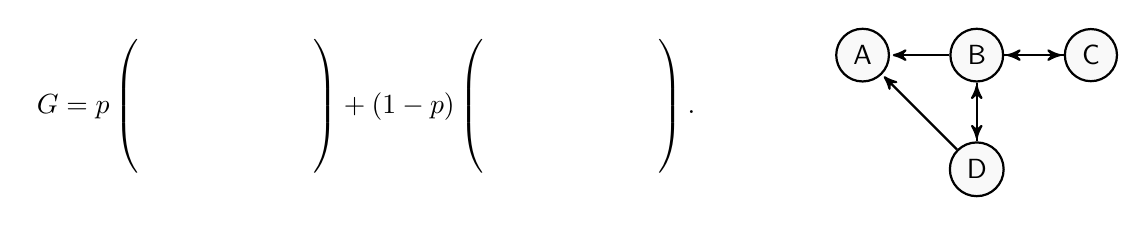
\begin{tikzpicture}
        \begin{scope}[->,>=stealth',shorten >=1pt,auto,node distance=1.45cm,thick, main node/.style={circle,fill=gray!05,draw}]
        \node[main node] (1) {A};
        \node[main node] (2) [right of=1] {B};
        \node[main node] (3) [below of=2] {D};
        \node[main node] (4) [right of=2] {C};
        \path[every node/.style={font=\sffamily\small}]
        (4) edge node[below] {} (2)
        (2) edge node [above] {} (1)
        edge [left] node {}  (3) 
        edge [left] node {}  (4) 
        (3) edge node {} (1)
        edge node[right] {} (2);
        %edge node[right] {} (5)
        %(4) edge node [above] {} (5)
        %(4) edge node [above] {} (5);
        \end{scope}
        \node[left] at (-2, -0.65) {$G = p\begin{pmatrix} &&&&&\\&\ &&&&\\&\ &&&&&\\&\ &&&&&\end{pmatrix} + (1-p)\begin{pmatrix} &&&&&\\&\ &&&&\\&\ &&&&&\\&\ &&&&&\end{pmatrix}.$};
    \end{tikzpicture}  
    \ifnum \Solutions=1 {\color{DarkBlue} \\ \textit{Solution:} The Google matrix is 
    $$G = p \begin{pmatrix} 
    1/4&1/3&0&1/2
    \\1/4&0&1&1/2
    \\1/4&1/3&0&0
    \\1/4&1/3&0&0 
    \end{pmatrix} + 
    (1-p)\begin{pmatrix}
    1/4&1/4&1/4&1/4\\
    1/4&1/4&1/4&1/4\\
    1/4&1/4&1/4&1/4\\
    1/4&1/4&1/4&1/4 
    \end{pmatrix}$$ 
    Note that we did not need to use the given value of $p$, which is ok. Also we could have written the answer (a bit) more neatly as: 
    $$G = p \begin{pmatrix} 
    1/4&1/3&0&1/2
    \\1/4&0&1&1/2
    \\1/4&1/3&0&0
    \\1/4&1/3&0&0 
    \end{pmatrix} + 
    \frac{(1-p)}{4}\begin{pmatrix}
    1&1&1&1\\
    1&1&1&1\\
    1&1&1&1\\
    1&1&1&1
    \end{pmatrix}$$     
    } \fi  
\fi 
\ifnum \Version=7 
    The steady-state probability vector for the Markov chain $\vec x_{k+1} = P\vec x_k$, where $k = 0,1,2,\ldots$ and $P=\dfrac15\begin{pmatrix} 3&1\\2&4\end{pmatrix}$ is $\vec q = \begin{pmatrix} c_1 \\c_2 \end{pmatrix}$, where $c_1 = \framebox{\strut\hspace{1cm}}$, $c_2 = \framebox{\strut\hspace{1cm}}$.
    \ifnum \Solutions=1 {\color{DarkBlue} \textit{Solution:} the steady state is a probability vector in the null space of $P-I$, and $$P-I = \begin{pmatrix} 3/5-1&1/5\\2/5&4/5-1 \end{pmatrix} \sim \begin{pmatrix} -2&1\\2&-1\end{pmatrix}$$ Then $\vec v = \begin{pmatrix} 1 & 2\end{pmatrix}^T$ is in the null space. But we need a probability vector. Dividing by the sum of the entries gives us the steady-state, $\vec q = \frac13 \begin{pmatrix} 1 & 2\end{pmatrix}^T$. So $c_1 = 1/3$, $c_2 = 2/3$. } \fi      
\fi 
\ifnum \Version=8
    $\lambda_1=3$ is an eigenvalue of $A$ with corresponding eigenvector $\vec v_1 = \begin{pmatrix} 5\\4\end{pmatrix}$. If $A\vec v_1 = \begin{pmatrix} c_1\\c_2\end{pmatrix}$, then $c_1 = \framebox{\strut\hspace{1cm}}$ and an eigenvalue of $A^2$ is \framebox{\strut\hspace{1cm}}. 
    
    \ifnum \Solutions=1 {\color{DarkBlue} \textit{Solution:} Since $\lambda_1$ is an eigenvalue of $A$, we must have that $$A\vec v_1 = \lambda_1 \vec v_1$$ Substituting the given information gives us $$A\vec v_1 = \lambda_1 \vec v_1 = 3 \begin{pmatrix} 5\\4 \end{pmatrix} = \begin{pmatrix} 15 \\ 12\end{pmatrix}$$  So $c_1 = 15$ and $c_2 = 12$. Moreover an eigenvalue of $A^2$ is 9. This is because we know that $A\vec v_1 = \lambda_1 \vec v_1$, so \begin{align}
        A\vec v_1 &= \lambda_1 \vec v_1 \\
        A(A\vec v_1) &= A(\lambda_1 \vec v_1) \\
        A^2\vec v_1 &= \lambda_1 A\vec v_1 \\
        A^2\vec v_1 &= \lambda_1^2 \vec v_1 
    \end{align}  } \fi    
\fi 
\ifnum \Version=9
    The area of the parallelogram with vertices at $(1,1)$, $(2,4)$, $(5,2)$, $(6,5)$ is \framebox{\strut\hspace{1cm}}. 
    \ifnum \Solutions=1 {\color{DarkBlue} \textit{Solution:} area is $\left| \det \begin{pmatrix} 1&4\\3&1\end{pmatrix} \right| = \left| 1\cdot1 - 3\cdot4 \right| = | 1 - 12 | = 12 - 1 = 11$. No credit for writing $-11$, as area cannot be negative. } \fi  
\fi 
\ifnum \Version=10
    If  $k$ is a  real number,  $A = \begin{pmatrix} 5&4\\k&k\end{pmatrix}$, $ B = \begin{pmatrix}15& k\\12 & k  \end{pmatrix}$, and $ \det A = 4$, then $\det B =  \framebox{\strut\hspace{1.2cm}}$ and $k= \framebox{\strut\hspace{1cm}}$.
    \ifnum \Solutions=1 {\color{DarkBlue} \textit{Solution:} matrix $B$ can be obtained from $A$ taking a transpose,  and multiplying a column by $3$. A transpose does not change the determinant.  Multiplying a column by $3$ multiplies the determinant by $3$. So $\det B = 12$. And if $\det A =4$, then \begin{align}
        \det A & = 4 \\
        \begin{vmatrix}
            5&4\\k&k 
        \end{vmatrix} &= 4 \\
        5k - 4k &= 4 \\
        k = 4
    \end{align}} \fi 
\fi 
\ifnum \Version=11
    $G$ is the Google Matrix for the set of four web pages that link to each other according to the diagram below. If the damping factor is $p=0.75$, fill in the missing entries of matrix $G$. 
    \vspace{4pt}
    
    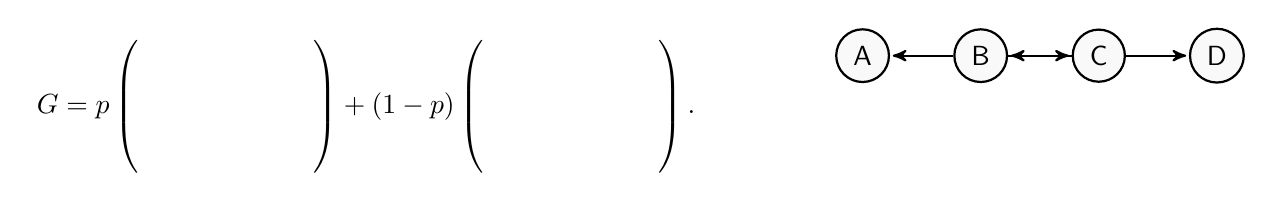
\begin{tikzpicture}
        \begin{scope}[->,>=stealth',shorten >=1pt,auto,node distance=1.5cm,thick, main node/.style={circle,fill=gray!05,draw}]
        \node[main node] (1) {A};
        \node[main node] (2) [right of=1] {B};
        \node[main node] (3) [right of=2] {C};
        \node[main node] (4) [right of=3] {D};
        \path[every node/.style={font=\sffamily\small}]
        (2) edge node [above] {} (1)
        edge [left] node {}  (3) 
        (3) edge node {} (2)
        edge node[right] {} (4);
        \end{scope}
        \node[left] at (-2, -0.65) {$G = p\begin{pmatrix} &&&&&\\&\ &&&&\\&\ &&&&&\\&\ &&&&&\end{pmatrix} + (1-p)\begin{pmatrix} &&&&&\\&\ &&&&\\&\ &&&&&\\&\ &&&&&\end{pmatrix}.$};
    \end{tikzpicture}  
    \ifnum \Solutions=1 {\color{DarkBlue} \\ \textit{Solution:} The Google matrix is 
    $$G = p \begin{pmatrix} 
    1/4&1/2&0&1/4\\
    1/4&0&1/2&1/4\\
    1/4&1/2&0&1/4\\
    1/4&0&1/2&1/4 
    \end{pmatrix} + 
    (1-p)\begin{pmatrix}
    1/4&1/4&1/4&1/4\\
    1/4&1/4&1/4&1/4\\
    1/4&1/4&1/4&1/4\\
    1/4&1/4&1/4&1/4 
    \end{pmatrix}$$ 
    Note that we did not need to use the given value of $p$, which is ok. Also we could have written the answer (a bit) more neatly as: 
    $$G = \frac p4 \begin{pmatrix} 
    1&2&0&1\\
    1&0&2&1\\
    1&2&0&1\\
    1&0&2&1 
    \end{pmatrix} + 
    \frac{(1-p)}{4}\begin{pmatrix}
    1&1&1&1\\
    1&1&1&1\\
    1&1&1&1\\
    1&1&1&1
    \end{pmatrix}$$     
    } \fi  
\fi 
\ifnum \Version=12
        Suppose that a $2\times 2$ matrix $A$ has eigenvalues $\lambda = 2$ and $\lambda= 3$. Then $\det(A^2) =  \framebox{\strut\hspace{1cm}}$. 
        \ifnum \Solutions=1 {\color{DarkBlue} \textit{Solution:} Using properties of determinants:
        \begin{align}
            \det(A^2) &= (\det A)^2 \\
            &= (\det (PDP^{-1}))^2 \\
            &= (\det P \det D \det P^{-1})^2\\
            &= (\det P  \det P^{-1} \det D)^2\\
            &= (\det (P P^{-1}) \det D)^4\\
            &= (\det (I) \det D)^2\\
            &= (\det D)^2
        \end{align}
        But $D$ is diagonal and its eigenvalues are 2 and 3, so $D$ is either 
        \begin{align}
            \begin{pmatrix} 3&0\\0&2\end{pmatrix} \quad \text{or} \quad \begin{pmatrix} 2&0\\0&3\end{pmatrix}
        \end{align}        
        Either way, $\det D = 3 \cdot 2 = 6$. So 
        \begin{align}
            \det(A^2) 
            &= (\det D)^2 = 6^2 = 36
        \end{align}        
        } \fi    
\fi 
\ifnum \Version=13 % 
    Let $S$ be an ellipse in whose area is 12. Then the area of $T(S)$, where $T(x) = Ax$, and $A = \begin{pmatrix} 2&4\\0&8\end{pmatrix}$ is \framebox{\strut\hspace{1cm}}.
    \ifnum \Solutions=1 {\color{DarkBlue} \textit{Solution:} The area of 
 is the area of the original ellipse 
, times the absolute value of the determinant of 
. We have
so area of 
 is   } \fi    
\fi 
\ifnum \Version=14 % 
    The steady-state vector of $P=\dfrac15\begin{pmatrix} 4&3\\1&2\end{pmatrix}$ is $\vec q = \begin{pmatrix} c_1 \\c_2 \end{pmatrix}$, where $c_1 = \framebox{\strut\hspace{1cm}}$, $c_2 = \framebox{\strut\hspace{1cm}}$.
        
    \ifnum \Solutions=1 {\color{DarkBlue} \textit{Solution:} the steady state is a probability vector in the null space of $P-I$, and $$P-I = \begin{pmatrix} 4/5-1&3/5\\1/5&2/5-1 \end{pmatrix} \sim \begin{pmatrix} -1&3\\1&-3\end{pmatrix}$$ Then $\begin{pmatrix} 3\\1\end{pmatrix}$ is in the null space. Dividing by the sum of the entries gives us the steady-state, $\vec q = \frac14 \begin{pmatrix} 3\\1\end{pmatrix}$. So $c_1 = 3/4, \ c_2 = 1/4$. } \fi   
\fi 
\ifnum \Version=15 % shouldn't need this version for fall 2023
    FILL IN THE BLANK ON UNIT 3
    \ifnum \Solutions=1 {\color{DarkBlue} \textit{Solution:} SOLUTION HERE  } \fi    
\fi 

\ifnum \Version=16 % shouldn't need this version for fall 2023
    FILL IN THE BLANK ON UNIT 3
    \ifnum \Solutions=1 {\color{DarkBlue} \textit{Solution:} SOLUTION HERE  } \fi    
\fi 

\ifnum \Version=17 % shouldn't need this version for fall 2023
    FILL IN THE BLANK ON UNIT 3
    \ifnum \Solutions=1 {\color{DarkBlue} \textit{Solution:} SOLUTION HERE  } \fi    
\fi 

\ifnum \Version=18 % shouldn't need this version for fall 2023
    FILL IN THE BLANK ON UNIT 3
    \ifnum \Solutions=1 {\color{DarkBlue} \textit{Solution:} SOLUTION HERE  } \fi    
\fi 




% \part Suppose $A$ is a $2\times 2$ matrix such that $\Nul A$ is the line $x_1-8x_2=0$, and a vector in $\Col A$ is $\vec u=\begin{pmatrix} 2\\4 \end{pmatrix}$. Then if $A=\begin{pmatrix}1 & c_1 \\ c_2 & c_3 \end{pmatrix} $, then $c_1= \framebox{\strut\hspace{1cm}}$, $c_2 =  \framebox{\strut\hspace{1cm}}$, and $c_3 =  \framebox{\strut\hspace{1cm}}$.

% \part If the LU factorization is $A=LU$, where $U$ is obtained by applying one row operation to $A$, and $A = \begin{pmatrix} 1&2&4\\3&2&12\end{pmatrix}$. Then $L = \begin{pmatrix} 1& 0\\l_1 & 1 \end{pmatrix} $ and $U= \begin{pmatrix} 1&2 & 4\\u_1 & u_2 & u_3 \end{pmatrix}$, where $l_1 = \framebox{\strut\hspace{1.25cm}}$, $u_1 = \framebox{\strut\hspace{1.25cm}}$, $u_2 = \framebox{\strut\hspace{1.25cm}}$ and $u_3 = \framebox{\strut\hspace{1.25cm}}$.


        % F) UNIT 4
\part 
\ifnum \Version=1
    Suppose $A$ has the QR factorization $A=QR$, where $A = \begin{pmatrix} 0&6\\1&0\\0&8\end{pmatrix}, \ Q = \begin{pmatrix} 0&\frac35\\1&0\\0&\frac45\end{pmatrix}$. 
    Then $R=\begin{pmatrix} r_1&r_2\\r_3&r_4\end{pmatrix}$, where 
    $r_1=\framebox{\strut\hspace{1cm}}$, 
    $r_2=\framebox{\strut\hspace{1cm}}$, 
    $r_3=\framebox{\strut\hspace{1cm}}$, 
    $r_4=\framebox{\strut\hspace{1cm}}$.
    \ifnum \Solutions=1 {\color{DarkBlue} \textit{Solution:} $R=Q^TA = \begin{pmatrix} 1&0\\0&10 \end{pmatrix}.$  } \fi    
\fi 
\ifnum \Version=2
    Vectors $u_1$ and $u_2$ form an orthogonal set. The projection of $y$ onto $S=\Span\{u_1,u_2\}$ is $\hat y = \proj_Sy$, where $y_1=\framebox{\strut\hspace{1cm}}$, 
    $y_2=\framebox{\strut\hspace{1cm}}$, $y_3=\framebox{\strut\hspace{1cm}}$. $$u_1 = \begin{pmatrix} 1\\2\\1\end{pmatrix}, \quad u_2 = \begin{pmatrix} 2\\-1\\0\end{pmatrix}, \quad y = \begin{pmatrix} 1\\0\\-1\end{pmatrix}, \quad \hat y = \begin{pmatrix} y_1\\y_2\\y_3\end{pmatrix}$$
    \ifnum \Solutions=1 {\color{DarkBlue} \textit{Solution:} the usual procedure yields
    \begin{align}
        \hat y &= \frac{y\cdot u_1}{u_1 \cdot u_1}u_1 + \frac{y\cdot u_2}{u_2 \cdot u_2}u_2 
        = 0 + \frac{2}{5}u_2
        = \begin{pmatrix} 4/5\\-2/5\\ 0\end{pmatrix} 
    \end{align}
    So $y_1=4/5, y_2=-2/5, y_3=0$. There are no other possible solutions.}
    \fi    
\fi 
\ifnum \Version=3
    An orthogonal basis for the subspace $S = \Span (y_1, y_2)$ is given by the set of vectors $\{\hat y_1, \hat y_2\}$, where $y_1 = \hat y_1$, $x_1 = \framebox{\strut\hspace{1cm}}$, $x_2 = \framebox{\strut\hspace{1cm}}$, and 
    $$
    y_1 = \hat y_1 = \begin{pmatrix} 2\\-5\\1\end{pmatrix}, \quad 
    y_2 = \begin{pmatrix} 8\\-2\\4\end{pmatrix}, \quad 
    \hat y_2 = \begin{pmatrix} x_1\\x_2\\ 3 \end{pmatrix}, \quad 
    $$
    
    \ifnum \Solutions=1 {\color{DarkBlue} \textit{Solution:} the usual procedure yields
    \begin{align}
        \hat y_2 
        &= y_2 - \frac{y_2\cdot y_1}{y_1 \cdot y_1}y_1 
        = \begin{pmatrix} 8\\-2\\4\end{pmatrix} - \frac{30}{30}\begin{pmatrix} 2\\-5\\1\end{pmatrix} 
        = \begin{pmatrix} 6\\3\\3\end{pmatrix}
    \end{align}
    So $x_1=6, x_2=3$. 
    } \fi    
\fi 
\ifnum \Version=4
    Vectors $u_1$ and $u_2$ form an orthogonal set. The projection of $y$ onto $S=\Span\{u_1,u_2\}$ is $\hat y = \proj_Sy$, where $y_1=\framebox{\strut\hspace{1cm}}$, 
    $y_2=\framebox{\strut\hspace{1cm}}$. $$u_1 = \begin{pmatrix} 1\\2\\2\end{pmatrix}, \quad u_2 = \begin{pmatrix} 2\\-1\\0\end{pmatrix}, \quad y = \begin{pmatrix} 1\\2\\11\end{pmatrix}, \quad \hat y = \begin{pmatrix} y_1\\y_2\\y_3\end{pmatrix}$$
    \ifnum \Solutions=1 {\color{DarkBlue} \textit{Solution:} the usual process yields
    \begin{align}
        \hat y &= \frac{y\cdot u_1}{u_1 \cdot u_1}u_1 + \frac{y\cdot u_2}{u_2 \cdot u_2}u_2 
        = \frac{27}{9}u_1 + 0u_2 = 3u_1 
        = \begin{pmatrix} 3\\6\\ 6\end{pmatrix} 
    \end{align}
    So $y_1=3, y_2=6, y_3=6$. There are no other possible solutions. } \fi  
\fi 
\ifnum \Version=5
    If matrix $A$ is $20\times 25$ and dim($(\Col A)\Perp$) = 5, the rank of $A$ is \framebox{\strut\hspace{1cm}}.
    \ifnum \Solutions=1 {\color{DarkBlue} \textit{Solution:} The answer is 15, because we are told that $5 = \dim ((\Col A)\Perp) = \dim(\Null (A^T))$. So $A^T$ has 5 non-pivotal columns, which means that $A$ has 5 non-pivotal rows. $A$ has 20 rows, so 15 rows are pivotal. And $\text{rank} A = \text{number of pivotal columns} = \text{number of pivotal rows} = 15$.   } \fi    
\fi 
\ifnum \Version=6
    The distance between $u=\begin{pmatrix} 5\\4\end{pmatrix}$ and the subspace $W=\text{Span}(v)$, where $v = \begin{pmatrix} 0\\1\end{pmatrix}$, is \framebox{\strut\hspace{1cm}}.     
    \ifnum \Solutions=1 {\color{DarkBlue} \textit{Solution:} 5. You might want to try sketching $u$ and the span of $v$ to see why the answer is 5.   } \fi    
\fi 
\ifnum \Version=7 
    Vectors $u_1$ and $u_2$ form an orthogonal set. The projection of $y$ onto $S=\Span\{u_1,u_2\}$ is $\hat y = \proj_Sy$, where $y_1=\framebox{\strut\hspace{1cm}}$, 
    $y_2=\framebox{\strut\hspace{1cm}}$. 
    $$
    u_1 = \begin{pmatrix} 3\\1\\0\end{pmatrix}, \quad 
    u_2 = \begin{pmatrix} 1\\-3\\2\end{pmatrix}, \quad 
    y = \begin{pmatrix} -1\\3\\12\end{pmatrix}, \quad 
    \hat y = \begin{pmatrix} y_1\\y_2\\y_3\end{pmatrix}
    $$
    \ifnum \Solutions=1 {\color{DarkBlue} \textit{Solution:} the usual process yields
    \begin{align}
        \hat y &= \frac{y\cdot u_1}{u_1 \cdot u_1}u_1 + \frac{y\cdot u_2}{u_2 \cdot u_2}u_2 
        = 0u_1 + \frac{14}{14}u_2 = u_2 
        = \begin{pmatrix} 1\\-3\\2\end{pmatrix} 
    \end{align}
    So $y_1=1, y_2=-3, y_3=2$. There are no other possible solutions. } \fi  
\fi 
\ifnum \Version=8
    The distance between $u=\begin{pmatrix} 3\\4\end{pmatrix}$ and the subspace $W=\text{Span}(v)$, where $v = \begin{pmatrix} 4\\-3\end{pmatrix}$, is \framebox{\strut\hspace{1cm}}.     
    \ifnum \Solutions=1 {\color{DarkBlue} \textit{Solution:} The distance is 5. Because the distance is given by $$\| y - \proj _W u \| = \| y - \frac{u\cdot v}{v\cdot v}v \| = \| y - 0 \| = \|y \| = 5$$.   } \fi    
\fi 
\ifnum \Version=9
    Vectors $u_1$ and $u_2$ form an orthogonal set. The projection of $y$ onto $S=\Span\{u_1,u_2\}$ is $\hat y = \proj_Sy$, where $y_1=\framebox{\strut\hspace{1cm}}$, 
    $y_2=\framebox{\strut\hspace{1cm}}$. $$u_1 = \begin{pmatrix} 1\\3\\2\end{pmatrix}, \quad u_2 = \begin{pmatrix} 3\\-1\\0\end{pmatrix}, \quad y = \begin{pmatrix} 4\\2\\2\end{pmatrix}, \quad \hat y = \begin{pmatrix} y_1\\y_2\\y_3\end{pmatrix}$$
    \ifnum \Solutions=1 {\color{DarkBlue} \textit{Solution:} the usual process yields
    \begin{align}
        \hat y &= \frac{y\cdot u_1}{u_1 \cdot u_1}u_1 + \frac{y\cdot u_2}{u_2 \cdot u_2}u_2 
        = \frac{14}{14}u_1 + \frac{10}{10}u_2 = u_1 + u_2 = \begin{pmatrix} 4\\2\\2\end{pmatrix}
    \end{align}
    So $y_1=4, y_2=2, y_3=2$. There are no other possible solutions. } \fi    
\fi 
\ifnum \Version=10
    Matrix $A = \begin{pmatrix} 0\\2\end{pmatrix}$ has the QR factorization $A = QR$, where $Q = \begin{pmatrix} q_1\\q_2\end{pmatrix}$, $R = r_1$, and 
    $q_1 = \framebox{\strut\hspace{1cm}}$, 
    $q_2 = \framebox{\strut\hspace{1cm}}$, 
    $r_1 = \framebox{\strut\hspace{1cm}}$.
    \ifnum \Solutions=1 {\color{DarkBlue} \textit{Solution:} the columns of $Q$ are an orthonormal basis for $\Col A$, so we can use $Q = \begin{pmatrix} 0\\1\end{pmatrix}$ or $Q = \begin{pmatrix} 0\\-1\end{pmatrix}$. And $R$ can be found using $R=Q^TA$. So 
    \begin{align}
        R = Q^TA = \begin{pmatrix} 0 & 1 \end{pmatrix}\begin{pmatrix} 0\\2\end{pmatrix} = 0 + 2 = 2
    \end{align} But we defined $R$ in such a way so that the entries on the main diagonal must be positive, so we can't use $Q = \begin{pmatrix} 0\\-1\end{pmatrix}$. So the only possible answer to this question is $q_1 = 0$, $q_2 = 1$, $r_1 = 2$.
    }\fi    
\fi 
\ifnum \Version=11
    Suppose $A$ has the QR factorization $A=QR$, where $A = \begin{pmatrix} 0&6\\1&0\\0&8\end{pmatrix}$. Then $Q = \begin{pmatrix} 0&3/5\\1&0\\0&4/5\end{pmatrix}$ and $R=\begin{pmatrix} r_1&r_2\\r_3&r_4\end{pmatrix}$, where 
    $r_1=\framebox{\strut\hspace{1cm}}$, 
    $r_2=\framebox{\strut\hspace{1cm}}$, 
    $r_3=\framebox{\strut\hspace{1cm}}$, 
    $r_4=\framebox{\strut\hspace{1cm}}$.
    
    \ifnum \Solutions=1 {\color{DarkBlue} We can use $R=Q^TA$. Performing the matrix multiplication:
    \begin{align}Q^TA &=  \begin{pmatrix} 0&1&0\\3/5&0&4/5\end{pmatrix} \begin{pmatrix} 0&6\\1&0\\0&8\end{pmatrix} \\
    &=  \begin{pmatrix} 0*0 + 1*1 + 0*0 & 0 \\ 0 & 3/5*6 + 0*0 + 4/5*8 \end{pmatrix} \\
    &= \begin{pmatrix} 1 & 0 \\ 0 & \frac{18+32}{5} \end{pmatrix} \\
    &= \begin{pmatrix} 1 & 0 \\ 0 & \frac{50}{5} \end{pmatrix} 
    \end{align}
    So $r_1 = 1$, $r_2=r_3=0$, $r_4=10$. Un-simplified fractions are acceptable. } \fi 
\fi 
\ifnum \Version=12
    Vectors $u_1$ and $u_2$ are an orthogonal basis for $S=\Span\{u_1,u_2\}$. The projection of $y$ onto $S$ is $\hat y = \proj_Sy$, where $y_1=\framebox{\strut\hspace{1cm}}$, 
    $y_2=\framebox{\strut\hspace{1cm}}$, $y_3 = \framebox{\strut\hspace{1cm}}$. $$u_1 = \begin{pmatrix} 2\\-4\\1\end{pmatrix}, \quad u_2 = \begin{pmatrix} 2\\1\\0\end{pmatrix}, \quad y = \begin{pmatrix} 4\\2\\21\end{pmatrix}, \quad \hat y = \begin{pmatrix} y_1\\y_2\\y_3\end{pmatrix}$$
    \ifnum \Solutions=1 {\color{DarkBlue} \textit{Solution:} the usual process yields
    \begin{align}
        \hat y 
        &= \frac{y\cdot u_1}{u_1 \cdot u_1}u_1 + \frac{y\cdot u_2}{u_2 \cdot u_2}u_2 
        = \frac{21}{21}u_1 + \frac{10}{5}u_2 = u_1 + 2u_2 
        =  \begin{pmatrix} 2\\-4\\1\end{pmatrix} + \begin{pmatrix} 4\\2\\0\end{pmatrix} 
        = \begin{pmatrix} 6\\-2\\1\end{pmatrix}
    \end{align}
    So $y_1=6, y_2=-2, y_3=1$. There are no other possible solutions. } \fi    
\fi 
\ifnum \Version=13
    An orthogonal basis for the subspace $S = \Span (y_1, y_2)$ is given by the set of vectors $\{\hat y_1, \hat y_2\}$, where $y_1 = \hat y_1$, $x_1 = \framebox{\strut\hspace{1cm}}$, $x_2 = \framebox{\strut\hspace{1cm}}$, and 
    $$
    y_1 = \hat y_1 = \begin{pmatrix} 2\\-5\\1\end{pmatrix}, \quad 
    y_2 = \begin{pmatrix} 8\\-2\\4\end{pmatrix}, \quad 
    \hat y_2 = \begin{pmatrix} x_1\\x_2\\ 3 \end{pmatrix}, \quad 
    $$
    
    \ifnum \Solutions=1 {\color{DarkBlue} \textit{Solution:} the usual procedure yields
    \begin{align}
        \hat y_2 
        &= y_2 - \frac{y_2\cdot y_1}{y_1 \cdot y_1}y_1 
        = \begin{pmatrix} 8\\-2\\4\end{pmatrix} - \frac{30}{30}\begin{pmatrix} 2\\-5\\1\end{pmatrix} 
        = \begin{pmatrix} 6\\3\\3\end{pmatrix}
    \end{align}
    So $x_1=6, x_2=3$. 
    } \fi    
\fi 
\ifnum \Version=14 % 
    Suppose $A$ has the QR factorization $A=QR$, where $A = \begin{pmatrix} 0&5\\1&0\\0&12\end{pmatrix}, \ Q = \begin{pmatrix} 0&\frac{5}{13}\\1&0\\0&\frac{12}{13}\end{pmatrix}$. 
    Then $R=\begin{pmatrix} r_1&r_2\\r_3&r_4\end{pmatrix}$, where 
    $r_1=\framebox{\strut\hspace{1cm}}$, 
    $r_2=\framebox{\strut\hspace{1cm}}$, 
    $r_3=\framebox{\strut\hspace{1cm}}$, 
    $r_4=\framebox{\strut\hspace{1cm}}$.
    \ifnum \Solutions=1 {\color{DarkBlue} \textit{Solution:} $R=Q^TA = \begin{pmatrix} 1&0\\0&13 \end{pmatrix}.$ So $r_1 = 1$, $r_2=r_3=0$, $r_4=13$.  } \fi    
\fi 
\ifnum \Version=15 % shouldn't need this version for fall 2023
    FILL IN THE BLANK ON UNIT 4
    \ifnum \Solutions=1 {\color{DarkBlue} \textit{Solution:} SOLUTION HERE  } \fi    
\fi 
\ifnum \Version=16 % shouldn't need this version for fall 2023
    FILL IN THE BLANK ON UNIT 4
    \ifnum \Solutions=1 {\color{DarkBlue} \textit{Solution:} SOLUTION HERE  } \fi    
\fi 
\ifnum \Version=17 % shouldn't need this version for fall 2023
    FILL IN THE BLANK ON UNIT 4
    \ifnum \Solutions=1 {\color{DarkBlue} \textit{Solution:} SOLUTION HERE  } \fi    
\fi 
\ifnum \Version=18 % shouldn't need this version for fall 2023
    FILL IN THE BLANK ON UNIT 4
    \ifnum \Solutions=1 {\color{DarkBlue} \textit{Solution:} SOLUTION HERE  } \fi    
\fi 

        % H) UNIT 5
\part
\ifnum \Version=1
    If $x \in \mathbb R^2$ and $A = \begin{pmatrix} 4&1\\1&4 \end{pmatrix}$, then the maximum value of $Q = x^TAx$, subject to the constraint $\|x\|=1$ is $Q = \framebox{\strut\hspace{1cm}}$. 

    \ifnum \Solutions=1 {\color{DarkBlue} \textit{Solution:} The eigenvalues of $A$ (by inspection) are $\lambda_1 = 3$ and $\lambda_2=5$. So the maximum value of $Q$ subject to the constraint is $\lambda_2 = 5$.   } \fi    
\fi 
\ifnum \Version=2

    If $x \in \mathbb R^2$ and $A = \begin{pmatrix} -2&1\\1&-2 \end{pmatrix}$, then the minimum value of $Q = x^TAx$, subject to the constraint $\|x\|=1$ is $Q = \framebox{\strut\hspace{1cm}}$. 

    \ifnum \Solutions=1 {\color{DarkBlue} \textit{Solution:} The eigenvalues of $A$ (by inspection) are $\lambda_1 = -3$ and $\lambda_2=-1$. So the minimum value of $Q$ subject to the constraint is $\lambda_2 = -3$.   } \fi        
\fi 
\ifnum \Version=3
    Suppose $A$ is a $2\times 2$ matrix with distinct eigenvalues, $A=A^T$, and $A$ has eigenvector $v_1$ corresponding to eigenvalue $\lambda_1$, where $v_1 = \begin{pmatrix} 1\\7 \end{pmatrix}$. If another eigenvector of $A$ is $v_2 = \begin{pmatrix} 21\\k\end{pmatrix}$, and $v_2$ corresponds to eigenvalue $\lambda_2$, where $\lambda_1 \ne \lambda_2$, then $k = \framebox{\strut\hspace{1cm}}$. 
    \ifnum \Solutions=1 {\color{DarkBlue} \textit{Solution:} $k=-3$.   } \fi    
\fi 
\ifnum \Version=4
    Suppose $A$ is an $2\times 2$ matrix and $A=A^T$. Suppose also that $x$ and $y$ are vectors in $\mathbb R^2$, and $Ax = 5x$ and $Ay = -y$. If $x=\begin{pmatrix} 3\\1\end{pmatrix}$, and $y=\begin{pmatrix} 4\\k\end{pmatrix}$, then $k=\framebox{\strut\hspace{1cm}}$. 
    \ifnum \Solutions=1 {\color{DarkBlue} \textit{Solution:} $k=-12$.  } \fi    
\fi 
\ifnum \Version=5
    The condition number of the matrix $A=\begin{pmatrix}-2&0\\0&6 \end{pmatrix}$ is 
        \framebox{\strut\hspace{1cm}}.
    \ifnum \Solutions=1 {\color{DarkBlue} \textit{Solution:} $A^TA = \begin{pmatrix} 4&0\\0&36\end{pmatrix}$, so $\sigma_1 = 6$, $\sigma_2 = 2$, and the condition number is $\kappa  = \frac{\sigma_1}{\sigma_2} = \frac 62 = 3$.   } \fi    
\fi 
\ifnum \Version=6
    If $A^TA = \begin{pmatrix} 3&1\\1&3 \end{pmatrix}$ then the maximum of $\|A\vec x\|$ subject to the constraint $\|\vec x\|=1$ is $\framebox{\strut\hspace{1cm}}$.
    \ifnum \Solutions=1 {\color{DarkBlue} \textit{Solution:}  The maximum of $\|A\vec x\|$ is the largest singular value of $A$, which are the square roots of the eigenvalues of $A^TA$. We could use the roots of the characteristic polynomial to obtain the eigenvalues, but it is faster to look for values of $\lambda$ that force $A - \lambda I$ to be singular (ie - dependent columns). By inspection the eigenvalues of $A^TA$ are $\lambda_1=4$ and $\lambda_2 = 2$. So $\sigma_1 = 2$, $\sigma_2 = \sqrt 2$. The largest singular value is 2, so the answer is 2. } \fi    
\fi 
\ifnum \Version=7
    If $A = \begin{pmatrix} 1&k\\k&0\end{pmatrix}$ and $\vec x = \begin{pmatrix} x_1\\x_2\end{pmatrix}$, then the quadratic form $Q = \vec x ^T A \vec x$ is positive semi-definite when $k = \framebox{\strut\hspace{1cm}}$. 
    
    \ifnum \Solutions=1 {\color{DarkBlue} \textit{Solution:} the form is positive semi-definite when all of the eigenvalues are non-negative. Note that:
    \begin{itemize}
        \item By inspection we can see that when $k=0$ that the form will be positive semi-definite because the matrix will be triangular with non-negative entries on the main diagonal. But are there any other values of $k$ that would work? 
        \item We can look at the eigenvalues of the matrix \(A = \begin{pmatrix} 1 & k \\ k & 0 \end{pmatrix}\). We solve the characteristic equation, which is given by
    \[ \text{det}\begin{pmatrix} 1-\lambda & k \\ k & -\lambda \end{pmatrix} = (1-\lambda)(-\lambda) - k^2 = \lambda^2 - \lambda - k^2 = 0 \]
    The solutions to this quadratic equation are the eigenvalues of matrix \(A\). They are
    $$\lambda = \frac12 \left( 1 \pm \sqrt{1 + 4 k^2}\right)$$ So when $k=0$ the eigenvalues are $1,0$. For all other values of $k$ there are two eigenvalues with opposite signs. When the eigenvalues have opposite signs the form is not positive semi-definite (it is indefinite). 
    \item The only value of $k$ that makes the form positive semi-definite is $k=0$. 
    \end{itemize}
    } \fi    
\fi 
\ifnum \Version=8
    If matrix $A$ has the SVD $A=U\Sigma V^T$, where $\Sigma = \begin{pmatrix} 3&0\\0&1\end{pmatrix}$, then the condition number of $A$ is $\kappa = \framebox{\strut\hspace{1cm}}$ and the dimension of $\Row A$ is $\framebox{\strut\hspace{1cm}}$.
    \ifnum \Solutions=1 {\color{DarkBlue} \textit{Solution:} the condition number is the ratio of the largest and smallest singular values, so $\kappa = 3/1 = 3$. The dimension of the row space is the number of pivot rows, which is 2. } \fi    
\fi 
\ifnum \Version=9
    The singular values of $A=\begin{pmatrix} 3&8\\-4&6\end{pmatrix}$ are $\sigma_1 = \framebox{\strut\hspace{1cm}}$ and $\sigma_2 = \framebox{\strut\hspace{1cm}}$. 
    
    \ifnum \Solutions=1 {\color{DarkBlue} \textit{Solution:} Singular values are the square roots of the eigenvalues of $A^TA$. So we can first compute \(A^TA\):
    \begin{align}
        A^TA = \begin{pmatrix} 3 & -4 \\ 8 & 6 \end{pmatrix} \begin{pmatrix} 3 & 8 \\ -4 & 6 \end{pmatrix} 
        = \begin{pmatrix} 9 + 16 & 24 - 24 \\ 24 - 24 & 64+36 \end{pmatrix}
        = \begin{pmatrix} 25 & 0 \\ 0 & 100 \end{pmatrix}
    \end{align} 
    
    The eigenvalues of \(A^TA\) could be obtained by solving the characteristic equation. But $A^TA$ happens to be triangular, so we can obtain the eigenvalues by inspection as $\lambda_1 = 100$ and $\lambda_2 = 25$. The singular values are the square roots of these numbers, so $\sigma_1 = 10$ and $\sigma_2 = 5$. Singular values are ordered from largest to smallest, so this is the only acceptable answer. } \fi    
\fi 
\ifnum \Version=10
    Suppose $A$ is an $2\times 2$ matrix and $A=A^T$. Suppose also that $x$ and $y$ are vectors in $\mathbb R^2$, and $Ax = 5x$ and $Ay = 3y$. If $x=\begin{pmatrix} 5\\-2\end{pmatrix}$, and $y=\begin{pmatrix} 12\\k\end{pmatrix}$, then $k=\framebox{\strut\hspace{1cm}}$. 
    \ifnum \Solutions=1 {\color{DarkBlue} \textit{Solution:} Given that \(A = A^T\), \(A\) is a symmetric matrix. The fact that \(Ax = 5x\) and \(Ay = 3y\) implies that \(x\) and \(y\) are eigenvectors of \(A\) with eigenvalues \(5\) and \(3\) respectively. The eigenvalues are distinct, Now, since \(A\) is symmetric, its eigenvectors are orthogonal. Therefore, \(v_1\) and \(v_2\) are orthogonal. If \(x\) and \(y\) are orthogonal vectors, their dot product is zero. The dot product of two vectors \(v\) and \(u\) is given by:
    \[ v \cdot u = v^T u \]
    In this case, if \(x\) and \(y\) are orthogonal, then:
    \[ x^T y = \begin{pmatrix} 5 & -2 \end{pmatrix} \begin{pmatrix} 12 \\ k \end{pmatrix} = 5 \cdot 12 + (-2) \cdot k = 60 - 2k = 0 \]
    Solving for \(k\):
    \begin{align*}
        60 - 2k &= 0 \\ 
        2k &= 60 \\
        k &= 30 
    \end{align*}
    Therefore, \(k\) must be \(30\). } \fi      
\fi 
\ifnum \Version=11
    The condition number of the matrix $A=\begin{pmatrix}-4&0\\0&8\end{pmatrix}$ is 
        \framebox{\strut\hspace{1cm}}.
    \ifnum \Solutions=1 {\color{DarkBlue} \textit{Solution:} $A^TA = \begin{pmatrix} 16&0\\0&64\end{pmatrix}$, so $\sigma_1 = \sqrt{64} = 8$, $\sigma_2 = \sqrt{16} = 4$, and the condition number is $\kappa  = \frac{\sigma_1}{\sigma_2} = \frac 84 = 2$.   } \fi      
\fi 
\ifnum \Version=12
    If $A$ is a real $2\times2$ matrix and $A^TA = \begin{pmatrix} 16&0\\0&1 \end{pmatrix}$, then the first right singular vector of $A$ is $\vec v_1 = \begin{pmatrix} c_1\\c_2\end{pmatrix}$, where $c_1 = \framebox{\strut\hspace{1cm}}$ and $c_2 = \framebox{\strut\hspace{1cm}}$. 
    \ifnum \Solutions=1 {\color{DarkBlue} \textit{Solution:} The right singular vectors are the unit eigenvectors of $A^TA$. The eigenvalues are $\lambda_1=16$ and $\lambda_2=1$. The first right singular vector will correspond to $\lambda_1 = 16$, and the vector will be a unit vector in the null space of $A^TA - \lambda_1I$. 
    \begin{align}
        A^TA - 16 I &= \begin{pmatrix} 0&0\\0&-15\end{pmatrix} 
    \end{align} So we can use $\vec v_1 = \begin{pmatrix} \pm 1 & 0\end{pmatrix}^T$. Thus $c_1$ can be either $+1$ or $-1$, but $c_2=0$.   } \fi    
\fi 
\ifnum \Version=13
    The condition number of the matrix $A=\begin{pmatrix}-2&0\\0&8 \end{pmatrix}$ is 
        \framebox{\strut\hspace{1cm}}.
    \ifnum \Solutions=1 {\color{DarkBlue} \textit{Solution:} $A^TA = \begin{pmatrix} 4&0\\0&64\end{pmatrix}$, so $\sigma_1 = 8$, $\sigma_2 = 2$, and the condition number is $\kappa  = \frac{\sigma_1}{\sigma_2} = \frac 82 = 4$.   } \fi    
\fi 
\ifnum \Version=14 % 
    Suppose $Q$ is the quadratic form \(Q = x^TAx\), where \(A\) is the symmetric matrix \(A = \begin{pmatrix} k & 4 \\ 4 & k \end{pmatrix}\) and $x = \begin{pmatrix} x_1\\x_2 \end{pmatrix}$. The quadratic form \(Q\) is positive definite when $k > \framebox{\strut\hspace{1cm}}$. 
    \ifnum \Solutions=1 {\color{DarkBlue} \textit{Solution:} the characteristic polynomial is 
    $$p(\lambda) 
    = \det(A - \lambda I) 
    = (k-\lambda)^2 - 4^2 
    = \lambda^2 -2k\lambda + k^2 - 16$$
    Then the roots are
    $$\lambda  = \frac{2k}{2} \pm \frac12 \sqrt{(2k)^2 - 4( k^2 - 16)} = k \pm \frac12 \sqrt{4\cdot 16} = k \pm 4$$
    The form is positive definite when the eigenvalues are all positive, which happens when $k > 4$.  } \fi    
\fi 
\ifnum \Version=15 % shouldn't need this version for fall 2023
    FILL IN THE BLANK ON UNIT 5
    \ifnum \Solutions=1 {\color{DarkBlue} \textit{Solution:} SOLUTION HERE  } \fi    
\fi 




        % C) U2

\ifnum \Version=1
    \part The LU factorization of $A = \begin{pmatrix} 2&5\\4&12\end{pmatrix}$ is $A=LU$, where $U$ is obtained by applying only one row operation to $A$. Then $U=\begin{pmatrix} 2&5\\u_1&u_2\end{pmatrix}$ and $L=\begin{pmatrix} l_1& 0\\l_2&l_3 \end{pmatrix}$, where 
    $u_1 = \framebox{\strut\hspace{1.00cm}}$, 
    $u_2 = \framebox{\strut\hspace{1.00cm}}$, 
    $l_1 = \framebox{\strut\hspace{1.00cm}}$, 
    $l_2 = \framebox{\strut\hspace{1.00cm}}$, and
    $l_3 = \framebox{\strut\hspace{1.00cm}}$. 
    \ifnum \Solutions=1 {\color{DarkBlue} \textit{Solution:} the only correct answer is $U=\begin{pmatrix} 2&5\\0&2 \end{pmatrix}$ and $L=\begin{pmatrix} 1&0\\2&1\end{pmatrix}$. } \fi 
\fi 

\ifnum \Version=2
    \part Suppose that we want reflect points in $\mathbb R^2$ across the line $x_1 = 4$. Using homogeneous coordinates we can use a transform of the form $T(\vec x) = A\vec x$, where $\vec x \in \mathbb R^3$ and $A$ is $$A = \begin{pmatrix} 1&0&a_1\\0&1&a_2\\0&0&a_3\end{pmatrix}\begin{pmatrix}b_1&b_2&0\\b_3&b_4&0\\0&0&1 \end{pmatrix}\begin{pmatrix} 1&0&c_1\\0&1&c_2\\0&0&c_3 \end{pmatrix}$$ Then $a_1 = \framebox{\strut\hspace{1.0cm}}$, $a_2 = \framebox{\strut\hspace{1.0cm}}$, $b_1 = \framebox{\strut\hspace{1.0cm}}$, $b_2 = \framebox{\strut\hspace{1.0cm}}$, $c_1 = \framebox{\strut\hspace{1.0cm}}$, $c_2 = \framebox{\strut\hspace{1.0cm}}$.
    \ifnum \Solutions=1 {\color{DarkBlue} \textit{Solutions.} 
    The matrices we need are
    $$A = \begin{pmatrix} 1&0&4\\0&1&0\\0&0&1\end{pmatrix}\begin{pmatrix}-1&0&0\\0&1&0\\0&0&1 \end{pmatrix}\begin{pmatrix} 1&0&-4\\0&1&0\\0&0&1 \end{pmatrix}$$    
    So $a_1 = 4, a_2 = 0, b_1 = -1, b_2 = 0, c_1 = -4, c_2 = 0$. 
    } 
    \fi    
\fi 
\ifnum \Version=3
    \part If $A = \begin{pmatrix} 1& 0 & 2 \\4&1&0\\0&0&1\end{pmatrix}$, then $A^{-1} = \begin{pmatrix} 1&0&c_1\\c_2&1&c_3\\0&0&1\end{pmatrix}$, where $c_1 = \framebox{\strut\hspace{.75cm}}$, $ c_2 = \framebox{\strut\hspace{.75cm}}$, $c_3 = \framebox{\strut\hspace{.75cm}}$. 
    \ifnum \Solutions=1 {\color{DarkBlue} \\[12pt] 
        There are a few ways to determine the values of the $c$'s. Here are a few methods. 
        \begin{itemize}
            \item Forming the augmented matrix $\begin{pmatrix}A \ | \ I\end{pmatrix}$ and reducing yields:
        \begin{align*}
            \begin{pmatrix}A \ | \ I\end{pmatrix} 
            = \begin{pmatrix} 1& 0 & 2 &1&0&0\\4&1&0&0&1&0\\0&0&1&0&0&1\end{pmatrix} 
            &\sim \begin{pmatrix} 1& 0 & 2 &1&0&0\\0&1&-8&-4&1&0\\0&0&1&0&0&1\end{pmatrix}\\
            &\sim \begin{pmatrix} 1& 0 & 2 &1&0&0\\0&1&0&-4&1&8\\0&0&1&0&0&1\end{pmatrix} \\
            &\sim \begin{pmatrix} 1& 0 & 0 &1&0&-2\\0&1&0&-4&1&8\\0&0&1&0&0&1\end{pmatrix}  = \begin{pmatrix}I \ | \ A^{-1}\end{pmatrix} 
        \end{align*}
        So $A^{-1} = \begin{pmatrix} 1&0&-2\\-4&1&8\\0&0&1\end{pmatrix}$ and $c_1 = -2, c_2 = -4, c_3 = 8$. 
        \item We could also set $AA^{-1} = I$ and solve for the unknowns. 
        \begin{align}
            AA^{-1} = \begin{pmatrix} 1& 0 & 2 \\4&1&0\\0&0&1\end{pmatrix}\begin{pmatrix} 1&0&c_1\\c_2&1&c_3\\0&0&1\end{pmatrix}
            &= \begin{pmatrix} 1&0&c_1+2\\4+c_2&1&4c_1+c_3\\0&0&1\end{pmatrix}
        \end{align}
        But $AA^{-1} = I$, so we have the equations
        \begin{align}
            c_1+2 &=0 \\
            4+c_2 &=0 \\
            4c_1 +c_3 &= 0
        \end{align}
        Solving these equations also gives us $c_1 = -2, c_2 = -4, c_3 = 8$.
        \end{itemize}
    } 
    \fi
\fi 
\ifnum \Version=4
    % Version 4 has a graphing question so skip 
\fi 
\ifnum \Version=5
    \part Suppose $A$, $B$, $C$ and $D$ are invertible $n\times n$ matrices, and $X= \begin{pmatrix} A & B\end{pmatrix}$, and $Y = \begin{pmatrix} C & D\end{pmatrix}$. If $XY^T=2AC^T$, then $D = \framebox{\strut\hspace{2cm}}$
    
    \ifnum \Solutions=1 {\color{DarkBlue} \textit{Solution:}  \begin{align}
        XY^T = \begin{pmatrix} A & B\end{pmatrix}\begin{pmatrix} C^T \\ D^T \end{pmatrix} & = 2AC^T\\
        AC^T + BD^T &= 2AC^T \\
        BD^T &= AC^T \\
        D^T &= B^{-1} AC^T \\
        D &= (B^{-1} AC^T)^T
    \end{align} It would also be ok to leave the answer as $D = CA^T(B^{-1})^T$.} \fi    
\fi 
\ifnum \Version=6
    \part If $A$ has LU factorization $A=LU$, where $U = \begin{pmatrix} 2&1\\0&3\end{pmatrix}$, and the solution to $L\vec y = \begin{pmatrix}6\\12 \end{pmatrix}$ is $\vec y = \begin{pmatrix} 2\\24 \end{pmatrix}$, then the solution to $A\vec x = \begin{pmatrix}6\\12 \end{pmatrix}$ is $\vec x = \begin{pmatrix} x_1\\x_2\end{pmatrix}$, where $x_1 = \framebox{\strut\hspace{1.0cm}}$, $x_2 = \framebox{\strut\hspace{1.0cm}}$.
    \ifnum \Solutions=1 {\color{DarkBlue} \textit{Solutions.} 
    If $A\vec x = LU\vec x = \begin{pmatrix} 6\\12 \end{pmatrix}$, and $L\vec y = \begin{pmatrix} 6\\12 \end{pmatrix}$ then $U\vec x = \vec y$. But we are given $\vec y$, so \begin{align} U\vec x = \begin{pmatrix} 2\\24 \end{pmatrix}\end{align} Expressing this as an augmented matrix we obtain 
    $$\begin{pmatrix} 2&1 & 2\\0&3&24 \end{pmatrix} \sim \begin{pmatrix} 2&1&2\\0&1&8\end{pmatrix} \sim \begin{pmatrix} 1&0&-3\\0&1&8\end{pmatrix}$$
    Thus $x_1 = -3$, $x_2= 8$. }
\fi
\fi 
\ifnum \Version=7
    \part The LU factorization of $A = \begin{pmatrix} 2&5\\4&12\end{pmatrix}$ is $A=LU$, where $U$ is obtained by applying only one row operation to $A$. Then $U=\begin{pmatrix} 2&5\\u_1&u_2\end{pmatrix}$ and $L=\begin{pmatrix} l_1& 0\\l_2&l_3 \end{pmatrix}$, where 
    $u_1 = \framebox{\strut\hspace{1.00cm}}$, 
    $u_2 = \framebox{\strut\hspace{1.00cm}}$, 
    $l_1 = \framebox{\strut\hspace{1.00cm}}$, 
    $l_2 = \framebox{\strut\hspace{1.00cm}}$, and
    $l_3 = \framebox{\strut\hspace{1.00cm}}$. 
    \ifnum \Solutions=1 {\color{DarkBlue} \textit{Solution:} the only correct answer is $U=\begin{pmatrix} 2&5\\0&2 \end{pmatrix}$ and $L=\begin{pmatrix} 1&0\\2&1\end{pmatrix}$. } \fi  
\fi 
\ifnum \Version=8
    \part If $A = \begin{pmatrix} 1& 0 & 3 \\4&1&0\\0&0&1\end{pmatrix}$, then $A^{-1} = \begin{pmatrix} 1&0&c_1\\c_2&1&c_3\\0&0&1\end{pmatrix}$, where $c_1 = \framebox{\strut\hspace{.75cm}}$, $ c_2 = \framebox{\strut\hspace{.75cm}}$, $c_3 = \framebox{\strut\hspace{.75cm}}$. 
    \ifnum \Solutions=1 {\color{DarkBlue} \\[12pt] 
        There are a few ways to determine the values of the $c$'s. Here are a few methods. 
        \begin{itemize}
            \item Forming the augmented matrix $\begin{pmatrix}A \ | \ I\end{pmatrix}$ and reducing yields:
        \begin{align*}
            \begin{pmatrix}A \ | \ I\end{pmatrix} 
            = \begin{pmatrix} 1& 0 & 3 &1&0&0\\4&1&0&0&1&0\\0&0&1&0&0&1\end{pmatrix} 
            &\sim \begin{pmatrix} 1& 0 & 3 &1&0&0\\0&1&-12&-4&1&0\\0&0&1&0&0&1\end{pmatrix}\\
            &\sim \begin{pmatrix} 1& 0 & 3 &1&0&0\\0&1&0&-4&1&12\\0&0&1&0&0&1\end{pmatrix} \\
            &\sim \begin{pmatrix} 1& 0 & 0 &1&0&-3\\0&1&0&-4&1&12j\\0&0&1&0&0&1\end{pmatrix}  = \begin{pmatrix}I \ | \ A^{-1}\end{pmatrix} 
        \end{align*}
        So $A^{-1} = \begin{pmatrix} 1&0&-3\\-4&1&8\\0&0&1\end{pmatrix}$ and $c_1 = -3, c_2 = -4, c_3 = 12$. 
        \item We could also set $AA^{-1} = I$ (or $A^{-1}A = I$), then multiply the matrices together, and then solve for the unknowns. The process should give the same values. 
        \end{itemize}
    } 
    \fi
\fi 
\ifnum \Version=9
    \part Determine all possible values of $k$ so that $AB=BA$, where $A = \begin{pmatrix} 2&k\\0&1\end{pmatrix}$ and $B = \begin{pmatrix} 1&-3\\0&2\end{pmatrix}$. $k = \framebox{\strut\hspace{1cm}}$. 
    \ifnum \Solutions=1 {\color{DarkBlue} \textit{Solution:} To determine all possible values of \(k\) such that \(AB = BA\) we can compute the products \(AB\) and \(BA\) and then set them equal to each other.
    \[ AB = \begin{pmatrix} 2 & k \\ 0 & 1 \end{pmatrix} \begin{pmatrix} 1 & -3 \\ 0 & 2 \end{pmatrix} =  \begin{pmatrix} 2 & -6 + 2k \\ 0 & 2 \end{pmatrix}.\]

    The product \(BA\) is:
    \[ BA = \begin{pmatrix} 1 & -3 \\ 0 & 2 \end{pmatrix} \begin{pmatrix} 2 & k \\ 0 & 1 \end{pmatrix} = \begin{pmatrix} 2 & k - 3 \\ 0 & 2 \end{pmatrix}.\]
    Now, we set \(AB = BA\) and compare the corresponding entries:
    \[ \begin{pmatrix} 2 & -6 + 2k \\ 0 & 2 \end{pmatrix} = \begin{pmatrix} 2 & k - 3 \\ 0 & 2 \end{pmatrix}.\]
    This leads to the following:
    \begin{align*}
    -6 + 2k &= k - 3, \\
    k & = 3
    \end{align*} 
     The only possible value of \(k\) is \(\boxed{3}\).
    } \fi    
\fi 
\ifnum \Version=10
    \part Suppose that we want reflect points in $\mathbb R^2$ across the line $x_2 = -3$. Using homogeneous coordinates we can use a transform of the form $T(\vec x) = A\vec x$, where $\vec x \in \mathbb R^3$ and $A$ is the matrix $$A = \begin{pmatrix} 1&0&a_1\\0&1&a_2\\0&0&a_3\end{pmatrix}\begin{pmatrix}b_1&b_2&0\\b_3&b_4&0\\0&0&1 \end{pmatrix}\begin{pmatrix} 1&0&c_1\\0&1&c_2\\0&0&c_3 \end{pmatrix}$$ Then 
    $a_1 = \framebox{\strut\hspace{1.00cm}}$, 
    $a_2 = \framebox{\strut\hspace{1.00cm}}$, 
    $b_1 = \framebox{\strut\hspace{1.00cm}}$, 
    $b_2 = \framebox{\strut\hspace{1.00cm}}$, 
    $c_1 = \framebox{\strut\hspace{1.00cm}}$, and 
    $c_2 = \framebox{\strut\hspace{1.00cm}}$.
    \ifnum \Solutions=1 {\color{DarkBlue} \textit{Solutions.} 
    The matrices we need are
    $$A = 
    \begin{pmatrix} 1&0&0\\0&1&-3\\0&0&1\end{pmatrix}
    \begin{pmatrix}1&0&0\\0&-1&0\\0&0&1 \end{pmatrix}
    \begin{pmatrix} 1&0&0\\0&1&3\\0&0&1 \end{pmatrix}$$    
    So $a_1 = 0, a_2 = -3, b_1 = 1, b_2 = 0, c_1 = 0, c_2 = 3$. 
    } 
    \fi       
\fi 
\ifnum \Version=11
    % no question needed here - will have a question 6
\fi 
\ifnum \Version=12
    % no question needed here - will have a question 6
\fi 
\ifnum \Version=13 % make-up
        % No problem needed because this version has a graphing problem 
\fi 
\ifnum \Version=14 % 
    \ifnum \Solutions=1 \newpage \fi
    \part If $A = \begin{pmatrix} 1& 0 & 0 \\4&1&0\\0&5&1\end{pmatrix}$, then $A^{-1} = \begin{pmatrix} 1&0&0\\c_1&1&0\\c_2&c_3&1\end{pmatrix}$, where $c_1 = \framebox{\strut\hspace{.75cm}}$, $ c_2 = \framebox{\strut\hspace{.75cm}}$, $c_3 = \framebox{\strut\hspace{.75cm}}$. 
    \ifnum \Solutions=1 {\color{DarkBlue} \\[12pt] 
        There are a few ways to determine the values of the $c$'s. Here are a few methods. 
        \begin{itemize}
            \item Forming the augmented matrix $\begin{pmatrix}A \ | \ I\end{pmatrix}$ and reducing yields:
        \begin{align*}
            \begin{pmatrix}A \ | \ I\end{pmatrix} 
            &= \begin{pmatrix} 1& 0 & 0 &1&0&0\\4&1&0&0&1&0\\0&5&1&0&0&1\end{pmatrix} \\
            &\sim \begin{pmatrix} 1& 0 & 0 &1&0&0\\0&1&0&-4&1&0\\0&5&1&0&0&1\end{pmatrix} \\
            &\sim \begin{pmatrix} 1& 0 & 0 &1&0&0\\0&1&0&-4&1&0\\0&5&1&20&-5&1\end{pmatrix} 
            = \begin{pmatrix}I \ | \ A^{-1}\end{pmatrix} 
        \end{align*}
        So $A^{-1} = \begin{pmatrix} 1&0&0\\-4&1&0\\20&-5&1\end{pmatrix}$ and $c_1 = -4, c_2 = 20, c_3 = -5$. 
        \item We could also set $AA^{-1} = I$ and solve for the unknowns. This approach should give the same result. 
        \end{itemize}
    } 
    \fi
\fi 
\ifnum \Version=15 % shouldn't need this version for fall 2023
    \part FILL IN THE BLANK ON UNIT 2
    \ifnum \Solutions=1 {\color{DarkBlue} \textit{Solution:} SOLUTION HERE  } \fi    
\fi 

        % G) UNIT 4 SOMETHING NOT ORTHOG COMP
\ifnum \Version=1
    \part If $A$ is a real $n \times n$ orthogonal matrix, $\vec x \in \mathbb R^n$ is a unit vector, then $||A^2 \, \vec x ||$ is equal to \framebox{\strut\hspace{1cm}}.
    \ifnum \Solutions=1 {\color{DarkBlue} \textit{Solution:} The answer is $1$. Because if we let $\vec y = A\vec x$, then: $$\|A^2\vec x \| = \|AA\vec x \| = \|A\vec y\| = \|\vec y\| = \|A\vec x\| = \|\vec x\| = 1$$ Note that the question states that $\vec x$ is a unit vector.   } \fi    
\fi 
\ifnum \Version=2
    \part A set of vectors are given to the Gram-Schmidt algorithm, which produces the vectors below. What must $h$ and $k$ be equal to? $h = \framebox{\strut\hspace{1cm}}, k = \framebox{\strut\hspace{1cm}}$ $$u=\begin{pmatrix} 1\\1\\0\\1\end{pmatrix}, \ v = \begin{pmatrix}1\\0\\1\\-1 \end{pmatrix}, \ w = \begin{pmatrix} 1\\2\\h\\k\end{pmatrix}$$
    \ifnum \Solutions=1 {\color{DarkBlue} \textit{Solution:} We need $u\cdot w=0$, so $$ 1+2+k=0$$ or $k=-3$. We also need $v\cdot w=0$, so $$1+h-k=1+h-(-3) = h+4=0$$ so $h=-4$. } \fi     
\fi 
\ifnum \Version=3
    \part If $A = \begin{pmatrix} 6&4\\a_1&a_2 \end{pmatrix}$, $y = \begin{pmatrix} 3\\4\end{pmatrix}$, $\proj_Wy = \begin{pmatrix} 4\\2\end{pmatrix}$, $W = \Col A$, then $a_1 = \framebox{\strut\hspace{0.80cm}}$ and $a_2 = \framebox{\strut\hspace{0.80cm}}$. 
    \ifnum \Solutions=1 {\color{DarkBlue} \textit{Solution:} $a_1= 3$, $a_2=2$. Because if $W = \Col(A)$ and $A$ is 2x2, then the columns of $A$ have to be linearly dependent. Otherwise if the columns of $A$ were independent, they would (in this case) span $\mathbb R^2$ and we would get $\text{proj}_Wy = y$. But we are told that $\text{proj}_Wy \ne y$ so the columns of $A$ must be dependent. Also, $\text{proj}_Wy$ is something in $W$. So the vector $\begin{pmatrix}4\\2 \end{pmatrix}$ must be in $W$. And so putting all of these ideas together: if $\begin{pmatrix}4\\2 \end{pmatrix}$ is in $W = \text{Col}A$, and the columns of $A$ are dependent, then set $A = \begin{pmatrix} 6&4\\3&2 \end{pmatrix}$.  } \fi    
\fi 
\ifnum \Version=4
    % No problem needed because Version 4 has a graphing problem 
\fi 
\ifnum \Version=5
  \part $A=\begin{pmatrix} 1 & 0 \\ 2 & -1\\ 2 & 1\end{pmatrix}$ has the QR factorization $A=QR$, where $Q= \begin{pmatrix} 1/3 &q_{12} \\q_{21} & q_{22}\\q_{31}& q_{32}\end{pmatrix}$, $R= \begin{pmatrix} r_{11} & r_{12} \\ r_{21} & r_{22}\end{pmatrix}$, where $q_{12}=\framebox{\strut\hspace{1cm}}$, $q_{22}=\framebox{\strut\hspace{1cm}}$, $q_{31}=\framebox{\strut\hspace{1cm}}$, $r_{11} = \framebox{\strut\hspace{1cm}}$, and $r_{22} = \framebox{\strut\hspace{1cm}}$. 
  \ifnum \Solutions=1 {\color{DarkBlue} \textit{Solutions.} 
    The columns of $Q$ form an orthonormal basis for $A$, but $A$ already has orthogonal columns, so we only need to normalize them to obtain $Q$. The columns of $Q$ are 
    \begin{align}
        \vec q_1 = \frac{1}{\sqrt{1^2+2^2+2^2}}\begin{pmatrix} 1\\2\\2\end{pmatrix} = \frac{1}{3}\begin{pmatrix} 1\\2\\2\end{pmatrix}, \quad \vec q_2 = \frac{1}{\sqrt{0^2+1^2+1^2}}\begin{pmatrix} 0\\-1\\1\end{pmatrix} = \frac{1}{\sqrt 2}\begin{pmatrix} 0\\-1\\1 \end{pmatrix} \end{align}
            And $R$ is obtained using \begin{align}
                R &= Q^TA = \begin{pmatrix} 1/3&2/3&2/3\\0&-1/\sqrt2& 1/\sqrt2\end{pmatrix}\begin{pmatrix} 1 & 0 \\ 2 & -1\\ 2 & 1\end{pmatrix} = \begin{pmatrix} 3&0\\0&2/\sqrt2 \end{pmatrix}
            \end{align}
            So $q_{12} = 0, q_{22} = -1/\sqrt2, q_{31} = 2/3$, and $r_{11} = 3, r_{22} = 2/\sqrt2$. 
    } 
   \else
      
   \fi
\fi 
\ifnum \Version=6
    \part If $D = \{ \vec x \in \mathbb R ^{3} \; | \;  x_1 - 4 x_2 + 5x_3 =0\}$, then an orthogonal basis for $D\Perp$ is  $\left\{ \hbox to 1.5cm{\vbox to 0.7cm{}} \right\}$
    \ifnum \Solutions=1 {\color{DarkBlue} \textit{Solution:} If $$\vec x = \begin{pmatrix}x_1\\x_2\\x_3 \end{pmatrix}$$ is a vector in $D$, then $0 = x_1 - 4x_2 +5x_3$. But we can re-write this using a dot product: 
            \begin{align*}
                0 &= x_1 - 4x_2 + 5x_3 = \begin{pmatrix} 1\\-4\\5 \end{pmatrix} \cdot \begin{pmatrix} x_1 \\ x_2\\x_3 \end{pmatrix} = \vec y \cdot \vec x, \quad \vec y = \begin{pmatrix} 1\\-4\\5 \end{pmatrix}
            \end{align*}
            Thus $\vec y \in D^{\perp}$. Moreover, $\Dim D = 2$, and the vectors in $D$ have three entries, so $\Dim D^{\perp}= 1$. So a basis for $D^{\perp}$ is given by $\vec y$, which we can denote as:
            $$\left\{ \begin{pmatrix} 1\\-4\\5 \end{pmatrix} \right\}$$
            Note that only round or square brackets should be used to denote a vector. Curly braces should only be used to denote sets in this course. An \textbf{incorrect} answer would be $$ \begin{Bmatrix} 1\\-4\\5 \end{Bmatrix} $$ } \fi   
\fi 
\ifnum \Version=7
    \part Suppose the least-squares solution to the inconsistent system $Ax=b$ is $\hat x$, where $x \in \mathbb R^2$, and $A$, $b$, and $\hat x$ are defined below. Then $x_1 = \framebox{\strut\hspace{1cm}}$, $x_2 = \framebox{\strut\hspace{1cm}}$.  $$A = \begin{pmatrix} 2&0\\0&5\\0&0\end{pmatrix}, \ b = \begin{pmatrix} 20\\10\\42\end{pmatrix}, \quad \hat x = \begin{pmatrix} x_1 \\ x_2\end{pmatrix}$$
    \ifnum \Solutions=1 {\color{DarkBlue} \textit{Solution:} using the normal equations 
    \begin{align}
        A^TA \hat x & = A^T b \\
        \begin{pmatrix} 2&0&0\\0&5&0 \end{pmatrix} \begin{pmatrix} 2&0\\0&5\\0&0\end{pmatrix} \hat x & = \begin{pmatrix} 2&0&0\\0&5&0 \end{pmatrix} \begin{pmatrix} 20\\10\\42\end{pmatrix} \\
        \begin{pmatrix} 4&0\\0&25\end{pmatrix} \hat x & = \begin{pmatrix} 40\\50 \end{pmatrix}
    \end{align}
    Thus $x_1 = 40/4 = 10$, and $x_2 = 50/25 = 2$. } \fi    
\fi 
\ifnum \Version=8
    \part If $u$ and $v$ are orthogonal vectors in $\mathbb R^n$ and the columns of $A$ are orthonormal, then the dot product $(Au)\cdot(Av) = \framebox{\strut\hspace{1cm}}$.
    \ifnum \Solutions=1 {\color{DarkBlue} \textit{Solution:} $(Au)\cdot(Av)=0$. Because  $$(Au)\cdot(Av) = (Au)^T(Av) = u^TA^TAv=u^TIv=u^Tv=0$$ } \fi    
\fi 
\ifnum \Version=9
    \part Suppose that $L$ is the line that passes through the point $(2,-4)$ and the origin. The orthogonal projection of $y = \begin{pmatrix} 7\\1\end{pmatrix}$ onto $L$ is $\hat y = \begin{pmatrix} c_1 \\ c_2 \end{pmatrix}$, where $c_1 = \framebox{\strut\hspace{1cm}}$ and $c_2 = \framebox{\strut\hspace{1cm}}$. 
    
    \ifnum \Solutions=1 {\color{DarkBlue} \textit{Solution:} For the given line \(L\) passing through the point \((2, -4)\) and the origin, a vector parallel to the line is $\mathbf{u} = \begin{pmatrix} 2 \\ -4 \end{pmatrix} $. The orthogonal projection of \(\mathbf{v}\) onto \(L\) is then:
    \[ \text{proj}_L(\mathbf{v}) 
    = \frac{y \cdot u}{\left\| u \right\|^2} u = \frac{7 \cdot 2 + 1 \cdot (-4)}{2^2 + (-4)^2} \cdot \begin{pmatrix} 2 \\ -4 \end{pmatrix} 
    = \frac{10}{20} \cdot \begin{pmatrix} 2 \\ -4 \end{pmatrix} 
    = \begin{pmatrix} 1 \\ -2 \end{pmatrix}. \]
    Therefore, the orthogonal projection of \(\begin{pmatrix} 7 \\ 1 \end{pmatrix}\) onto the line \(L\) is \(\begin{pmatrix} 1 \\ -2 \end{pmatrix}\). So $c_1 = 1$, $c_2 = -2$.  } \fi    
\fi 
\ifnum \Version=10
    \part Suppose matrix $A$ has the QR factorization $A = QR$, and the least-squares solution to the inconsistent system $Ax=b$ is $\hat x$, where $x \in \mathbb R^2$, and $A$, $b$, and $\hat x$ are defined below. Then $x_1 = \framebox{\strut\hspace{1cm}}$, $x_2 = \framebox{\strut\hspace{1cm}}$. $$Q= \frac15 \begin{pmatrix} 4&-3\\3&4\end{pmatrix}, R = \begin{pmatrix} 1&0\\0&3\end{pmatrix}, \ \ b = \begin{pmatrix} 5\\15\end{pmatrix}, \ \hat x = \begin{pmatrix} x_1 \\ x_2\end{pmatrix}$$
    \ifnum \Solutions=1 {\color{DarkBlue} \textit{Solution:} the least-squares solution is given by the solution to $R\hat x = Q^Tb$. And 
    $$Q^Tb 
    = \frac15 \begin{pmatrix} 4&3\\-3&4\end{pmatrix} \begin{pmatrix} 5\\15\end{pmatrix} 
    = \frac15 \begin{pmatrix} 65 \\ 45\end{pmatrix} = \begin{pmatrix} 13\\9\end{pmatrix}$$
    The system $R\hat x = Q^Tb$ has the augmented matrix below. 
    $$\begin{pmatrix} 1&0&13\\0&3&9\end{pmatrix}$$
    Thus $x_1 = 13$, $x_2 = 3$. 
    } \fi    
\fi 
\ifnum \Version=11
    % no question needed here - will have a graphing question 
\fi 
\ifnum \Version=12
    % no question needed here - will have a graphing question
\fi 
\ifnum \Version=13 % make-up
        % No problem needed because this version has a graphing problem 
\fi 
\ifnum \Version=14 % 
    \part If $x = \begin{pmatrix} 6\\4 \end{pmatrix}$, $v = \begin{pmatrix} 1\\3\end{pmatrix}$, $V = \text{Span}\{v\}$, then $\proj_V x = \begin{pmatrix} c_1\\c_2\end{pmatrix}$, where $c_1 = \framebox{\strut\hspace{0.75cm}}$ and $c_2 = \framebox{\strut\hspace{0.75cm}}$. 
    \ifnum \Solutions=1 {\color{DarkBlue} \textit{Solution:} the projection formula gives us 
    $$\proj_V x 
    = \frac{x\cdot v}{v\cdot v} v 
    = \frac{6+12}{1+9}\begin{pmatrix} 1\\3\end{pmatrix} 
    = \frac{18}{10}\begin{pmatrix} 1\\3\end{pmatrix} 
    = \begin{pmatrix} 9/5\\27/5\end{pmatrix} 
    $$ Therefore $c_1 = 9/5$, and $c_2 = 27/5$.} \fi    
\fi 
\ifnum \Version=15 % shouldn't need this version for fall 2023
    \part FILL IN THE BLANK ON UNIT 4
    \ifnum \Solutions=1 {\color{DarkBlue} \textit{Solution:} SOLUTION HERE  } \fi    
\fi 
\ifnum \Version=16 % shouldn't need this version for fall 2023
    \part FILL IN THE BLANK ON UNIT 4
    \ifnum \Solutions=1 {\color{DarkBlue} \textit{Solution:} SOLUTION HERE  } \fi    
\fi 
\ifnum \Version=17 % shouldn't need this version for fall 2023
    \part FILL IN THE BLANK ON UNIT 4
    \ifnum \Solutions=1 {\color{DarkBlue} \textit{Solution:} SOLUTION HERE  } \fi    
\fi 
\ifnum \Version=18 % shouldn't need this version for fall 2023
    \part FILL IN THE BLANK ON UNIT 4
    \ifnum \Solutions=1 {\color{DarkBlue} \textit{Solution:} SOLUTION HERE  } \fi    
\fi 

    \end{parts}
\fi 
\ifnum \SetNumber = 2
    \begin{parts} 
        % A) UNIT 1 TRANSFORMS
\part 
\ifnum \Version=1
    If $A$ is $2 \times 2$ and $T_A(\vec x)=A\vec x$ is a linear transform that first rotates points clockwise in $\mathbb R^2$ about the origin by $\pi/2$ radians and then reflects them through the line $x_2 = 0$, then $A=\begin{pmatrix} a_1 & a_2 \\ a_3 & a_4 \end{pmatrix} $ where $a_1 = \framebox{\strut\hspace{1.0cm}}$, $a_2 = \framebox{\strut\hspace{1.0cm}}$, $a_3 = \framebox{\strut\hspace{1.0cm}}$ and $a_4 = \framebox{\strut\hspace{1.0cm}}$.
    
    \ifnum \Solutions=1 {\color{DarkBlue} \textit{Solutions.} 
    Using $A = \begin{pmatrix} T(e_1) & T(e_2) \end{pmatrix}$, we obtain
    \begin{align}
        e_1 &= \begin{pmatrix} 1\\0 \end{pmatrix} \to \begin{pmatrix}0\\-1 \end{pmatrix} \to \begin{pmatrix}0\\1 \end{pmatrix} \\
        e_2 &= \begin{pmatrix} 0 \\1 \end{pmatrix} \to \begin{pmatrix} 1\\0 \end{pmatrix} \to \begin{pmatrix}1\\0 \end{pmatrix}
    \end{align}
    Thus $A = \begin{pmatrix} T(e_1) & T(e_2) \end{pmatrix} = \begin{pmatrix} 0 & 1\\1 & 0\end{pmatrix}$, so $a_1=0$, $a_2=1$, $a_3=1$, $a_4=0$. 
    } 
    \else
    \fi    
\fi 

\ifnum \Version=2
        If the transform $T_A(\vec x) = A\vec x$ is onto, where $T_A \ : \ \mathbb R^{12} \to \mathbb R^9$, then $A$ has exactly $\framebox{\strut\hspace{0.80cm}}$ pivots, the domain of $T_A$ is $\framebox{\strut\hspace{0.80cm}}$, the co-domain of $T_A$ is $\framebox{\strut\hspace{0.80cm}}$, and the range of $T_A$ is $\framebox{\strut\hspace{0.80cm}}$. 
        
        \ifnum \Solutions=1 {\color{DarkBlue} \textit{Solutions.} 
        If the transform is onto, every row must be pivotal. So there are 9 pivots, the domain is $\mathbb R^{12}$, the co-domain is $\mathbb R^9$, and the range is also $\mathbb R^9$. It would \textbf{not} be correct to say that the domain is $12$ and that the co-domain is $9$. 
        } 
       \fi      
\fi 

\ifnum \Version=3
    If $A$ is $2 \times 2$ and $T_A(\vec x)=A\vec x$ is a linear transform that first rotates points counter-clockwise in $\mathbb R^2$ about the origin by $\pi/2$ radians and then reflects them through the line $x_1 = 0$, then $A=\begin{pmatrix} a_1 & a_2 \\ a_3 & a_4 \end{pmatrix} $ where $a_1 = \framebox{\strut\hspace{1.0cm}}$, $a_2 = \framebox{\strut\hspace{1.0cm}}$, $a_3 = \framebox{\strut\hspace{1.0cm}}$ and $a_4 = \framebox{\strut\hspace{1.0cm}}$.
    
    \ifnum \Solutions=1 {\color{DarkBlue} \textit{Solutions.} 
    Using $A = \begin{pmatrix} T(e_1) & T(e_2) \end{pmatrix}$, we obtain
    \begin{align}
        e_1 &= \begin{pmatrix} 1\\0 \end{pmatrix} \to \begin{pmatrix}0\\1 \end{pmatrix} \to \begin{pmatrix}0\\1 \end{pmatrix} \\
        e_2 &= \begin{pmatrix} 0 \\1 \end{pmatrix} \to \begin{pmatrix} -1\\0 \end{pmatrix} \to \begin{pmatrix}1\\0 \end{pmatrix}
    \end{align}
    Thus $A = \begin{pmatrix} T(e_1) & T(e_2) \end{pmatrix} = \begin{pmatrix} 0 & 1\\1 & 0\end{pmatrix}$, so $a_1=0$, $a_2=1$, $a_3=1$, $a_4=0$. 
    } 
    \else
    \fi        
\fi 


\ifnum \Version=4
        If the transform $T_A(\vec x) = A\vec x$ is one-to-one, where $T_A \ : \ \mathbb R^{8} \to \mathbb R^{14}$, then $A$ has exactly $\framebox{\strut\hspace{1.00cm}}$ pivots, the domain of $T_A$ is \framebox{\strut\hspace{1.00cm}}, the co-domain of $T_A$ is $\framebox{\strut\hspace{1.00cm}}$, and the range of $T_A$ is a subspace of $\mathbb R^p$, where $p = \framebox{\strut\hspace{1.00cm}}$. 
        
        \ifnum \Solutions=1 {\color{DarkBlue} \textit{Solutions.} 
        If the transform is one-to-one, every column must be pivotal. So there are 8 pivots, the domain is $\mathbb R^{8}$, the co-domain is $\mathbb R^{14}$, and the range is a subspace of $\mathbb R^{14}$. It would \textbf{not} be correct to say that the domain is $8$ and that the co-domain is $14$. $8$ is a number, $\mathbb R^8$ is a set. 
        } 
       \fi      
\fi 
\ifnum \Version=5
        If the transform $T_A(\vec x) = A\vec x$ is onto, where $T_A \ : \ \mathbb R^6 \to \mathbb R^4$, then $A$ has exactly $\framebox{\strut\hspace{1.00cm}}$ pivots, the domain of $T_A$ is \framebox{\strut\hspace{1.00cm}}, the co-domain of $T_A$ is $\framebox{\strut\hspace{1.00cm}}$, and the range of $T_A$ is $\framebox{\strut\hspace{1.00cm}}$. 
        
        \ifnum \Solutions=1 {\color{DarkBlue} \textit{Solutions.} 
        The standard matrix of the transform must be $4\times6$. If the transform is onto, every row must be pivotal. So there are 4 pivots, the domain is $\mathbb R^6$, the co-domain is $\mathbb R^4$, and the range is also $\mathbb R^4$. It would \textbf{not} be correct to say that the domain is $6$ and that the co-domain is $4$. 
        } 
       \fi    
\fi 
\ifnum \Version=6
    Suppose $A$, $B$, and $C$ are $2\times2$ matrices, $A = BC$, and $B$ is the standard matrix for a transform that projects vectors in $\mathbb R^2$ onto the $x_1$-axis. If $T(\vec x)=C\vec x$ rotates vectors clockwise by $\pi/2$ radians about the origin, then $\Null A$ is spanned by $\vec y = \begin{pmatrix} y_1\\y_2\end{pmatrix}$ where $y_1 = \framebox{\strut\hspace{1.0cm}}$ and $y_2 = \framebox{\strut\hspace{1.0cm}}$. Please use numbers for $y_1$ and $y_2$ (not variables). 
    
    \ifnum \Solutions=1 {\color{DarkBlue} \textit{Solutions.} 
    Note that $B = \begin{pmatrix} 1&0\\0&0\end{pmatrix}$, so the nullspace of $B$ is the line $x_1= 0$. Note also that the line $x_1=0$ is the $x_2$-axis, and that there are a few ways to approach this problem. Here are a few different methods. 
    \begin{itemize}
        \item \textbf{Method 1}: The transform $T(x) = Ax = BCx$ first rotates vectors clockwise by $\pi/2$ radians about the origin. Any vector on the $x_1$-axis gets rotated to the $x_2$-axis. Vectors on the $x_1$-axis are in the span of $y = \begin{pmatrix} 1\\0 \end{pmatrix}$. So any vector in the span of $y$ is rotated into $\Null B$, so $BCy = 0$. But $A=BC$ so $\Null A$ is spanned by $y = \begin{pmatrix} 1\\0\end{pmatrix}$. We can choose $y_1 = 1$ and $y_2=0$. 
        % \item \textbf{Method 2}: The transform $T(x) = Ax = BCx$ first rotates vectors clockwise by $\pi/2$ radians about the origin. In other words, $C$ will transform $e_1 = \begin{pmatrix} 1\\0 \end{pmatrix}$ to $T_C(e_1) = \begin{pmatrix} 0\\-1 \end{pmatrix}$, and $e_2 = \begin{pmatrix} 0\\ 1 \end{pmatrix}$ to $T_C(e_2) = \begin{pmatrix} 1\\0 \end{pmatrix}$. This means that the standard matrix of the transform $T_C$ is $C = \begin{pmatrix} 0&1\\-1&0\end{pmatrix}$, and $C$ will transform a vector of the form $\begin{pmatrix}x_1\\x_2 \end{pmatrix}$ to $\begin{pmatrix} x_2 \\ -x_1\end{pmatrix}$. But $\Null B$ is the line spanned by $\begin{pmatrix} 0\\1\end{pmatrix}$, so $T_C(x)$ is in $\Null B$ when $x_2 = 0$. So $y = \begin{pmatrix} x_1 \\ x_2 \end{pmatrix} = \begin{pmatrix}x_1\\0 \end{pmatrix}$. So we can choose $y_1 = 1$ and $y_2 = 0$. 
        \item \textbf{Method 2}: Using the general form of a rotation matrix, $C$ is $$C = \begin{pmatrix} 0&1\\-1&0\end{pmatrix}$$
        But $T(x) = Ax = BCx$, and so
        $$BC = \begin{pmatrix} 1&0\\0&0\end{pmatrix}\begin{pmatrix} 0&1\\-1&0\end{pmatrix} = \begin{pmatrix} 0 & 1 \\ 0&0\end{pmatrix}$$
        A vector in the null space of this matrix is $y = \begin{pmatrix} 1\\0\end{pmatrix}$. We can choose $y_1 = 1$ and $y_2=0$. 
    \end{itemize}
    Do not leave your answer as $y_1 = x_1$ and $y_2=0$ because then you haven't specified that $x_1 \ne 0$. 
    } 
    \fi    

\fi 
\ifnum \Version=7
    If $A$ is $2 \times 2$ and $T_A(\vec x)=A\vec x$ is a linear transform that first rotates points counter-clockwise in $\mathbb R^2$ about the origin by $\pi$ radians and then reflects them through the line $x_1+x_2 = 0$, then $A=\begin{pmatrix} a_1 & a_2 \\ a_3 & a_4 \end{pmatrix} $ where $a_1 = \framebox{\strut\hspace{1.0cm}}$, $a_2 = \framebox{\strut\hspace{1.0cm}}$, $a_3 = \framebox{\strut\hspace{1.0cm}}$ and $a_4 = \framebox{\strut\hspace{1.0cm}}$.
    
    \ifnum \Solutions=1 {\color{DarkBlue} \textit{Solutions.} 
    Using $A = \begin{pmatrix} T(e_1) & T(e_2) \end{pmatrix}$, we obtain
    \begin{align}
        e_1 &= \begin{pmatrix} 1\\0 \end{pmatrix} \to \begin{pmatrix}-1\\0 \end{pmatrix} \to \begin{pmatrix}0\\1 \end{pmatrix} \\
        e_2 &= \begin{pmatrix} 0 \\1 \end{pmatrix} \to \begin{pmatrix} 0\\-1 \end{pmatrix} \to \begin{pmatrix}1\\0 \end{pmatrix}
    \end{align}
    Thus $A = \begin{pmatrix} T(e_1) & T(e_2) \end{pmatrix} = \begin{pmatrix} 0 & 1\\1 & 0\end{pmatrix}$, so $a_1=0$, $a_2=1$, $a_3=1$, $a_4=0$. 
    } 
    \else
    \fi    
\fi 
\ifnum \Version=8
    Let $T \, : \, \mathbb R^2 \to \mathbb R^2$ be a linear transform such that $T(x_1,x_2) = (x_1+x_2, 2x_2)$, and $b = \begin{pmatrix} 5& 4\end{pmatrix}^T$, and $\vec x= \begin{pmatrix} x_1,x_2 \end{pmatrix}^T$. Then $T(\vec x) = b$ when $x_1 = \framebox{\strut\hspace{1cm}}$ and $x_2 = \framebox{\strut\hspace{1cm}}$. 
    
    \ifnum \Solutions=1 {\color{DarkBlue} \textit{Solution:} The standard matrix of the transform is $A = \begin{pmatrix} 1&1\\0&2\end{pmatrix}$, so $Ax = b$, or as an augmented matrix: 
    \begin{align}
        \begin{pmatrix}1&1&5\\0&2&4 \end{pmatrix}
        \sim \begin{pmatrix}1&1&5\\0&1&2 \end{pmatrix}
        \sim \begin{pmatrix}1&0&3\\0&1&2 \end{pmatrix}
    \end{align} 
    So $x_1 =3$, $x_2 = 2$. }\fi    
\fi 
\ifnum \Version=9
     Suppose $e_1 = \begin{pmatrix}1\\0 \end{pmatrix}$, $e_2 = \begin{pmatrix} 0\\1\end{pmatrix}$, and $T \, : \, \mathbb R^2 \to \mathbb R^2$ is a linear transform such that $T(e_1) = \begin{pmatrix} 2\\0 \end{pmatrix}$, and $T(e_2) = \begin{pmatrix} -3\\2\end{pmatrix}$. If $x = \begin{pmatrix} c_1 \\ c_2 \end{pmatrix}$, and $T(x) = b = \begin{pmatrix} 2\\ 4\end{pmatrix}$, then $c_1 = \framebox{\strut\hspace{0.75cm}}$ and $c_2 = \framebox{\strut\hspace{0.75cm}}$. 
     
    \ifnum \Solutions=1 {\color{DarkBlue} \textit{Solution:} The standard matrix of the transform is $$A = \begin{pmatrix}2&-3\\0&2 \end{pmatrix}$$ But if $Ax=b$, then we may solve: 
    \begin{align}
        \begin{pmatrix} A \, | \, b \end{pmatrix} &= \begin{pmatrix} 2&-3&2\\0&2&4\end{pmatrix}
        \sim \begin{pmatrix} 2&-3&2\\0&1&2\end{pmatrix} 
        \sim \begin{pmatrix} 2&0&8\\0&1&2\end{pmatrix} 
        \sim \begin{pmatrix} 1&0&4\\0&1&2\end{pmatrix} 
    \end{align} So $c_1 = 4$ and $c_2 = 2$.} \fi    
\fi 
\ifnum \Version=10
      If $A$ is $2 \times 2$ and $T_A(\vec x)=A\vec x$ is a linear transform that first rotates points in $\mathbb R^2$ counter-clockwise about the origin by $\pi/2$ radians and then reflects them through the line $x_1 = 0$, then $A=\begin{pmatrix} a_1 & a_2 \\ a_3 & a_4 \end{pmatrix} $ where $a_1 = \framebox{\strut\hspace{1.25cm}}$, $a_2 = \framebox{\strut\hspace{1.25cm}}$, $a_3 = \framebox{\strut\hspace{1.25cm}}$ and $a_4 = \framebox{\strut\hspace{1.25cm}}$.

        \ifnum \Solutions=1 {\color{DarkBlue} \textit{Solutions.} 
            Using $A = \begin{pmatrix} T(e_1) & T(e_2) \end{pmatrix}$, we obtain
            \begin{align}
                e_1 &= \begin{pmatrix} 1\\0 \end{pmatrix} \to \begin{pmatrix}0\\1 \end{pmatrix} \\
                e_2 &= \begin{pmatrix} 0 \\1 \end{pmatrix} \to \begin{pmatrix} 1\\0 \end{pmatrix}
            \end{align}
            Thus $A = \begin{pmatrix} T(e_1) & T(e_2) \end{pmatrix} = \begin{pmatrix} 0 & 1\\1 & 0\end{pmatrix}$, so $a_1=0$, $a_2=1$, $a_3=1$, $a_4=0$. 
        } 
       \fi
\fi 
\ifnum \Version=11
    Let $T \, : \, \mathbb R^2 \to \mathbb R^2$ be a linear transformation that maps
    $u = \begin{pmatrix} 3\\2 \end{pmatrix}$ to $T(u) = \begin{pmatrix} 4\\5\end{pmatrix}$ and maps $v = \begin{pmatrix}8\\-2 \end{pmatrix}$ to $T(v) = \begin{pmatrix} 2\\1\end{pmatrix}$. Then $T(2u+3v) = \begin{pmatrix} c_1\\c_2\end{pmatrix}$, where $c_1 = \framebox{\strut\hspace{1cm}}$ and $c_2 = \framebox{\strut\hspace{1cm}}$.  
    \ifnum \Solutions=1 {\color{DarkBlue} \textit{Solution:} Using linearity, $$T(2u+3v) = 2T(u) + 3T(v) = 2\begin{pmatrix} 4\\5\end{pmatrix} + 3\begin{pmatrix} 2\\1\end{pmatrix} = \begin{pmatrix} 14\\13\end{pmatrix}$$ So $c_1 = 14$, $c_2 = 13$.  } \fi    
\fi 
\ifnum \Version=12
    Let $\vec x = \begin{pmatrix} x_1 \\x_2\end{pmatrix}$, $\vec v_1 = \begin{pmatrix} 9\\56\end{pmatrix}$, and $\vec v_2 = \begin{pmatrix} 15\\23\end{pmatrix}$. Let $T \, : \, \mathbb R^2 \to \mathbb R^2$ be a linear transformation that maps $\vec x$ to $T(\vec x) = x_1 \vec v_1 + x_2 \vec v_2$. Then a matrix $A$ that $T(\vec x) = A\vec x$ for every $\vec x$ in the domain of $T$ is $A = \begin{pmatrix} a_1&a_2\\a_3&a_4\end{pmatrix}$, where $a_1 = \framebox{\strut\hspace{1cm}}$, $a_2 = \framebox{\strut\hspace{1cm}}$, $a_3 = \framebox{\strut\hspace{1cm}}$, $a_4 = \framebox{\strut\hspace{1cm}}$. 
    \ifnum \Solutions=1 {\color{DarkBlue} \textit{Solution:} take $\vec x$ to be the standard vectors $\vec e_1$ and $\vec e_2$ to obtain the columns of $A$. 
    \begin{align}
        T(\vec e_1) &= A\vec e_1 = 1\cdot \vec v_1 + 0 \cdot \vec v_2 = \vec v_1 \\
        T(\vec e_2) &= A\vec e_2 = 0\cdot \vec v_1 + 1 \cdot \vec v_2 = \vec v_2 \\
        A &= \begin{pmatrix} \vec v_1 & \vec v_2 \end{pmatrix} = \begin{pmatrix} 9&15\\56&23\end{pmatrix}
    \end{align}
    So $a_1 = 9, a_2 = 15, a_3=56, a_4=23$. 
    } \fi
\fi 
\ifnum \Version=13 % 
    % DONE
    Let $T \, : \, \mathbb R^2 \to \mathbb R^2$ be a linear transformation that maps
    $u=\begin{pmatrix} 1\\6 \end{pmatrix}$ into $T(u) = \begin{pmatrix} 2\\15\end{pmatrix}$ and maps $v=\begin{pmatrix} 3\\5\end{pmatrix}$ to $T(v) = \begin{pmatrix} 5\\4\end{pmatrix}$. Then $T(2u+3v) = \begin{pmatrix} c_1\\c_2\end{pmatrix}$, where $c_1 = \framebox{\strut\hspace{1cm}}$ and $c_2 = \framebox{\strut\hspace{1cm}}$.  
    \ifnum \Solutions=1 {\color{DarkBlue} \textit{Solution:} Using linearity, $$T(2u+3v) = 2T(u) + 3T(v) = 2\begin{pmatrix} 2\\15\end{pmatrix} + 3\begin{pmatrix} 5\\4 \end{pmatrix} = \begin{pmatrix}19\\42 \end{pmatrix}$$  } \fi    
\fi 
\ifnum \Version=14 % 
    Suppose $\vec v_1= \begin{pmatrix}3\\0\\5 \end{pmatrix}$, $\vec v_2 = \begin{pmatrix}1\\1\\0 \end{pmatrix}$, and $\vec y = \begin{pmatrix} 2\\c_1\\c_2\end{pmatrix}$. If $A$ has 2 pivots, the transform $T(\vec x)=A\vec x$ satisfies $T(\vec v_1) = 2T(\vec v_2) \ne \vec 0$, and $\vec y$ satisfies $A\vec y = \vec 0$, then $c_1 = \framebox{\strut\hspace{1cm}}$, $c_2 = \framebox{\strut\hspace{1cm}}$.  
    \ifnum \Solutions=1 {\color{DarkBlue} \textit{Solutions.} 
        Let the columns of $A$ be $a_1, a_2, a_3$. Then using linearity: 
        \begin{align}
            T(\vec v_1) &= 2T(\vec v_2) \\
            0 & = T(\vec v_1) - 2T(\vec v_2) \\
            0 & = T(\vec v_1 - 2\vec v_2) \\
            0 & = T\left( \begin{pmatrix}3\\0\\5 \end{pmatrix}- 2 \begin{pmatrix}1\\1\\0 \end{pmatrix} \right) \\
            0 & = T\left( \begin{pmatrix}2\\-2\\5 \end{pmatrix}\right) \\
            0 & = A y , \ \text{where } y = \begin{pmatrix}2\\-2\\5 \end{pmatrix} 
        \end{align}
        So $c_1 = -2$, and $c_2 = 5$. 
        } 
   \else
   \fi 
\fi 
\ifnum \Version=15 % shouldn't need this version for fall 2023
    Suppose $A = \begin{pmatrix} 3 & 0\\3 & 1\end{pmatrix}$ and the image of $x= \begin{pmatrix} c_1 \\ c_2 \end{pmatrix}$ under the transform $T(x) = Ax$ is $b = \begin{pmatrix} 6\\7\end{pmatrix}$, then $c_1 = \framebox{\strut\hspace{1cm}}$ and $c_2 = \framebox{\strut\hspace{1cm}}$. 
    \ifnum \Solutions=1 {\color{DarkBlue} \textit{Solution:} We need to solve $Ax=b$. Expressing as an augmented matrix and row reducing yields
    $$\begin{pmatrix} 3&0&6\\3&1&7\end{pmatrix} 
    \sim \begin{pmatrix} 1&0&2\\3&1&7\end{pmatrix} 
    \sim \begin{pmatrix} 1&0&2\\0&1&1\end{pmatrix} 
    $$ So $c_1 = 2$ and $c_2 = 1$.} \fi  
\fi 
\ifnum \Version=16 % shouldn't need this version for fall 2023
    FILL IN THE BLANK ON UNIT 1 LINEAR TRANSFORMS
    \ifnum \Solutions=1 {\color{DarkBlue} \textit{Solution:} SOLUTION HERE  } \fi    
\fi 
\ifnum \Version=17 % shouldn't need this version for fall 2023
    FILL IN THE BLANK ON UNIT 1 LINEAR TRANSFORMS
    \ifnum \Solutions=1 {\color{DarkBlue} \textit{Solution:} SOLUTION HERE  } \fi    
\fi 
\ifnum \Version=18 % shouldn't need this version for fall 2023
    FILL IN THE BLANK ON UNIT 1 LINEAR TRANSFORMS
    \ifnum \Solutions=1 {\color{DarkBlue} \textit{Solution:} SOLUTION HERE  } \fi    
\fi 

        % D) Unit 2
\part 
\ifnum \Version=1
    
    If $A = \begin{pmatrix} 4&a_1\\a_2&a_3\end{pmatrix}$, $\Col A$ is the line $x_1=2x_2$, $\Null A$ is the line $x_1=3x_2$, then 
    $a_1 = \framebox{\strut\hspace{1.0cm}}$ and 
    $a_2 = \framebox{\strut\hspace{1.0cm}}$. 
    
    \ifnum \Solutions=1 {\color{DarkBlue} \textit{Solutions.} 
    If $\Col A$ is the line $x_1=2x_2$ then a vector in $\Col A$ is $\begin{pmatrix} 4\\2\end{pmatrix}$ because if $x_2=2$, then $x_1=4$. Then the first column of $A$ can be $\begin{pmatrix} 4\\2\end{pmatrix}$ or $A = \begin{pmatrix} 4&a_1\\2&a_3\end{pmatrix}$. We need to work out what $a_1$ is, but if $\Null A$ is the line $x_1-3x_2=0$ then a vector in the null space of $A$ is $v = \begin{pmatrix} 3\\1\end{pmatrix}$, so $$Av = \begin{pmatrix}4&a_1\\2&a_3 \end{pmatrix}\begin{pmatrix} 3\\1\end{pmatrix} = \begin{pmatrix} 0\\0\end{pmatrix}$$ This gives us $12+a_1=0$. So $a_1 = -12$ and $a_2 = 2$.
    } 
   \else
   \fi            
\fi 
\ifnum \Version=2
    If $S = \{\vec x \in \mathbb R^5 \, | \, x_1+x_2 = 0, x_3=x_4\}$, then $\dim S = \framebox{\strut\hspace{1cm}}$ and $\dim (S^{\perp}) = \framebox{\strut\hspace{1.0cm}}$. 
    \ifnum \Solutions=1 {\color{DarkBlue} \textit{Solution:} $\dim S = 3$ and $\dim (S^{\perp}) = 2$.  } \fi     
\fi 
\ifnum \Version=3
    If $S = \{\vec x \in \mathbb R^3 \, | \, x_1+x_2 = 0\}$, then $\dim S = \framebox{\strut\hspace{1cm}}$ and $v = \begin{pmatrix} 4&h&k\end{pmatrix}^T$ is in $S$ when $h = \framebox{\strut\hspace{1.0cm}}$. 
    \ifnum \Solutions=1 {\color{DarkBlue} \textit{Solution:} $\dim S = 2$ and $h = -4$.  } \fi    
\fi 
\ifnum \Version=4 If the consumption matrix for an economy is $C=\frac{1}{10}\begin{pmatrix} 3&0\\2&9\end{pmatrix}$ then the output $x$ to meet a desired output $d=\begin{pmatrix} 14\\20\end{pmatrix}$ is $x=\begin{pmatrix} x_1\\x_2 \end{pmatrix}$, where $x_1 = \framebox{\strut\hspace{1.0cm}}$, $x_2 = \framebox{\strut\hspace{1.0cm}}$.

\ifnum \Solutions=1 {\color{DarkBlue} \textit{Solutions:} 
The output we need satisfies 
$$x = d + Cx$$
Which is also
$$(I-C)x = d$$
But 
$$I-C = \begin{pmatrix} 1&0\\0&1\end{pmatrix} - \begin{pmatrix} 0.3 & 0 \\ 0.2 & 0.9 \end{pmatrix} = \begin{pmatrix} 0.7 & 0 \\ -0.2 & 0.1 \end{pmatrix}$$
Thus we can determine $x$ by reducing the augmented matrix below as follows. 
\begin{align}
    \begin{pmatrix} 0.7 & 0 & 14\\ -0.2 &  0.1 & 20\end{pmatrix} 
    & \sim \begin{pmatrix} 7 & 0 & 140\\ -2 & 1 & 200\end{pmatrix} 
     \sim \begin{pmatrix} 1 & 0 & 20\\ -2 & 1 & 200\end{pmatrix} 
     \sim \begin{pmatrix} 1 & 0 & 20\\ 0 & 1 & 240\end{pmatrix} 
\end{align}
Thus $x_1 = 20$, $x_2 = 240$. 
} 
\fi        
\fi 

\ifnum \Version=5
    If $x = \begin{pmatrix} 10\\22\end{pmatrix}$, $S=\{v_1,v_2\}$, $v_1=\begin{pmatrix} 1\\2\end{pmatrix}, v_2 = \begin{pmatrix} 3\\7\end{pmatrix}$, then $[x]_S = \begin{pmatrix} c_1\\c_2\end{pmatrix}$ is the coordinate vector relative to the basis $S$, where $c_1 = \framebox{\strut\hspace{1cm}}$ and $c_2 = \framebox{\strut\hspace{1cm}}$. 
    \ifnum \Solutions=1 {\color{DarkBlue} \\[12pt] The entries of the coordinate vector are the coefficients in the basis given by the vectors in $S$. In other words, we can determine $c_1$ and $c_2$ by solving 
    $$c_1v_1 + c_2v_2 = x$$
    Reducing the corresponding augmented matrix: 
    $$\begin{pmatrix} 1&3&10\\2&7&22\end{pmatrix} 
    \sim \begin{pmatrix} 1&3&10\\0&1&2\end{pmatrix}
    \sim \begin{pmatrix} 1&0&4\\0&1&2\end{pmatrix}$$
    So the coordinate vector is $[x]_S = \begin{pmatrix} 4\\2\end{pmatrix}$ and $c_1 = 4$, $c_2 = 2$. 
    } 
    \fi
\fi 
\ifnum \Version=6
    How many vectors are needed to form a basis for the subspace $\{\vec x \in \mathbb R^3 \, | \, x_1+x_2 = 0\}$? $\framebox{\strut\hspace{1.0cm}}$. 

    \ifnum \Solutions=1 {\color{DarkBlue} Two vectors are needed to form a basis.  } \fi    
\fi 
\ifnum \Version=7
    If $A = \begin{pmatrix} 30&a_1\\a_2&a_3\end{pmatrix}$, $\Col A$ is the subspace $\{ \vec x \in \mathbb R^2 \, | \, x_1 = 2x_2\}$, $\Null A$ is the line $x_1+3x_2=0$, then $a_1 = \framebox{\strut\hspace{1.0cm}}$ and $a_2 = \framebox{\strut\hspace{1.0cm}}$. 
    
    \ifnum \Solutions=1 {\color{DarkBlue} \textit{Solutions.} The answers are $a_1= 90, a_2 = 15$. Because if $\Col A$ is the subspace $x_1=2x_2$ then a vector in $\Col A$ is $\begin{pmatrix} 30\\15\end{pmatrix}$ because if $x_2=15$, then $x_1=30$. Then the first column of $A$ can be $\begin{pmatrix} 30\\15\end{pmatrix}$ or $A = \begin{pmatrix} 30 & a_1\\ 15 & a_3\end{pmatrix}$. We need to work out what $a_1$ is, but if $\Null A$ is the line $x_1+3x_2=0$ then the point $(3,-1)$ is on this line, which means that a vector in the null space of $A$ is $v = \begin{pmatrix} 3\\-1\end{pmatrix}$. So $$Av = \begin{pmatrix}30&a_1\\15&a_3 \end{pmatrix}\begin{pmatrix} 3\\-1\end{pmatrix} = \begin{pmatrix} 0\\0\end{pmatrix}$$ This gives us $90-a_1=0$. So $a_1 = 90$. A similar process would give us that $a_3 = 45$.
    } 
   \else
   \fi     
\fi 
\ifnum \Version=8
    If $S = \{\vec x \in \mathbb R^5 \, | \, x_1+x_2 = 0, x_3=x_5\}$, then $\dim S = \framebox{\strut\hspace{1cm}}$ and a vector in $S$ is $(0 \ 0 \ 5 \ 3 \ k)^T$, where $k = \framebox{\strut\hspace{1cm}}$. 
    \ifnum \Solutions=1 {\color{DarkBlue} \textit{Solution:} $\dim S = 3$ and $k=5$.  } \fi    
\fi 
\ifnum \Version=9
If $A = \begin{pmatrix} 2&5\\3&8\end{pmatrix}$ and $A^{-1} = \begin{pmatrix} a_1 & a_2 \\ a_3 & a_4 \end{pmatrix}$, then $a_1 = \framebox{\strut\hspace{0.75cm}}$, $a_2 = \framebox{\strut\hspace{0.75cm}}$, $a_3 = \framebox{\strut\hspace{0.75cm}}$, $a_4 = \framebox{\strut\hspace{0.75cm}}$.
    
    \ifnum \Solutions=1 {\color{DarkBlue} \textit{Solutions:} We can either use the formula for the inverse of a $2\times 2 $ matrix or row reduce the block matrix $\begin{pmatrix} A & I\end{pmatrix}$. The latter yields
    \begin{align}
        \begin{pmatrix} A & I\end{pmatrix} 
        = \begin{pmatrix} 2&5&1&0\\3&8&0&1\end{pmatrix} 
        &\sim \begin{pmatrix} 2&5&1&0\\0&1/2&-3/2&1\end{pmatrix}\\
        &\sim \begin{pmatrix} 2&5&1&0\\0&1&-3&2\end{pmatrix}\\
        &\sim \begin{pmatrix} 2&0&16&-10\\0&1&-3&2\end{pmatrix}\\
        &\sim \begin{pmatrix} 1&0&8&-5\\0&1&-3&2\end{pmatrix}
    \end{align}
    Thus $A^{-1} =\begin{pmatrix} 8&-5\\-3&2\end{pmatrix}$. 
    } 
    \fi        
\fi 
\ifnum \Version=10
    If $x = \begin{pmatrix} 5\\7\\12\end{pmatrix}$, $S=\{v_1,v_2\}$, $v_1=\begin{pmatrix} -1\\1\\2\end{pmatrix}, v_2 = \begin{pmatrix} 4\\2\\3\end{pmatrix}$, then $[x]_S = \begin{pmatrix} c_1\\c_2\end{pmatrix}$ is the coordinate vector relative to the basis $S$, where $c_1 = \framebox{\strut\hspace{1cm}}$ and $c_2 = \framebox{\strut\hspace{1cm}}$. 
    \ifnum \Solutions=1 {\color{DarkBlue} \\[12pt] The entries of the coordinate vector are the coefficients in the basis given by the vectors in $S$. In other words, we can determine $c_1$ and $c_2$ by solving 
    $$c_1v_1 + c_2v_2 = x$$
    Reducing the corresponding augmented matrix: 
    $$
    \begin{pmatrix} -1&4&5\\1&2&7\\2&3&12\end{pmatrix} 
    \sim \begin{pmatrix} -1&4&5\\0&6&12\\0&11&22\end{pmatrix} 
    \sim \begin{pmatrix} 1&-4&-5\\0&1&2\\0&0&0\end{pmatrix} 
    \sim \begin{pmatrix} 1&0&3\\0&1&2\\0&0&0\end{pmatrix} 
    $$
    So the coordinate vector is $[x]_S = \begin{pmatrix} 3\\2\end{pmatrix}$ and $c_1 = 3$, $c_2 = 2$. 
    } 
    \fi  
\fi 
\ifnum \Version=11
    If $A = \begin{pmatrix} a_1&4\\a_2&a_3\end{pmatrix}$, $\Col A$ is the line $x_2=3x_1$, $\Null A$ is the line $5x_1+x_2=0$, then 
    $a_1 = \framebox{\strut\hspace{1.0cm}}$ and 
    $a_3 = \framebox{\strut\hspace{1.0cm}}$. 
    
    \ifnum \Solutions=1 {\color{DarkBlue} \textit{Solutions.} $a_1=20, a_3=12$. Because if $\Col A$ is the line $x_2=3x_1$ then a vector in $\Col A$ is $\begin{pmatrix} 4\\12\end{pmatrix}$ because if $x_1=4$, then $x_2=12$. Then the second column of $A$ can be $\begin{pmatrix} 4\\12\end{pmatrix}$ or $A = \begin{pmatrix} a_1&4\\a_2&12\end{pmatrix}$. If $\Null A$ is the line $5x_1+x_2=0$ then a vector in the null space of $A$ is $v = \begin{pmatrix} 1\\-5\end{pmatrix}$, so $Av = \begin{pmatrix}a_1&4\\a_2&12 \end{pmatrix}\begin{pmatrix} 1\\-5\end{pmatrix} = \begin{pmatrix} 0\\0\end{pmatrix}$. This gives us $a_1=20$.
    } 
      
   \fi        
\fi 
\ifnum \Version=12
    If $A = \begin{pmatrix} 1&a_1\\a_2&a_3\end{pmatrix}$, $\Col A$ is the line $x_2=2x_1$, $\Null A$ is the line $x_1+4x_2=0$, then 
    $a_1 = \framebox{\strut\hspace{1.0cm}}$, 
    $a_2 = \framebox{\strut\hspace{1.0cm}}$, 
    $a_3 = \framebox{\strut\hspace{1.0cm}}$. 
    
    \ifnum \Solutions=1 {\color{DarkBlue} \textit{Solutions.} 
    If $\Col A$ is the line $x_2=2x_1$ then a vector in $\Col A$ is $\begin{pmatrix} 1\\2\end{pmatrix}$ because if $x_1=1$, then $x_2=2$. Then the first column of $A$ can be $\begin{pmatrix} 1\\2\end{pmatrix}$ or $A = \begin{pmatrix} 1&c_1\\2&c_2\end{pmatrix}$. We need to work out what $c_1$ and $c_2$ are, but if $\Null A$ is the line $x_1+4x_2=0$ then a vector in the null space of $A$ is $v = \begin{pmatrix} 4\\-1\end{pmatrix}$, so $$Av = \begin{pmatrix}1&c_1\\2&c_2 \end{pmatrix}\begin{pmatrix} 4\\-1\end{pmatrix} = \begin{pmatrix} 0\\0\end{pmatrix}$$ This gives us $4-c_1 = 0$, $2\cdot 4-c_2 = 0$, so $c_1 = 4$, $c_2 = 8$. And
    $$A = \begin{pmatrix} 1&4\\2&8\end{pmatrix}$$ 

    } 
   \else 
      
   \fi        
\fi 
\ifnum \Version=13 % 
    If $x = \begin{pmatrix} 7\\1\\0\end{pmatrix}$, $S=\{v_1,v_2\}$, $v_1=\begin{pmatrix} 3\\1\\2\end{pmatrix}, v_2 = \begin{pmatrix} 4\\2\\5\end{pmatrix}$, then $[x]_S = \begin{pmatrix} c_1\\c_2\end{pmatrix}$ is the coordinate vector relative to the basis $S$, where $c_1 = \framebox{\strut\hspace{1cm}}$ and $c_2 = \framebox{\strut\hspace{1cm}}$. 
    \ifnum \Solutions=1 {\color{DarkBlue} \\[12pt] The entries of the coordinate vector are the coefficients in the basis given by the vectors in $S$. In other words, we can determine $c_1$ and $c_2$ by solving 
    $$c_1v_1 + c_2v_2 = x$$
    Reducing the corresponding augmented matrix: FIX NUMBERS
    $$\begin{pmatrix} 3&4&7\\1&2&1\\2&5&0\end{pmatrix} 
    \sim \begin{pmatrix} 1&3&10\\0&1&2\end{pmatrix}
    \sim \begin{pmatrix} 1&0&4\\0&1&2\end{pmatrix}$$
    So the coordinate vector is $[x]_S = \begin{pmatrix} 4\\2\end{pmatrix}$ and $c_1 = 4$, $c_2 = 2$. 
    } 
    \fi
\fi 
\ifnum \Version=14 % 
    If the consumption matrix for an economy is $C=\frac{1}{10}\begin{pmatrix} 6&2\\0&4\end{pmatrix}$ then the output $x$ to meet a desired output $d=\begin{pmatrix} 14\\20\end{pmatrix}$ is $x=\begin{pmatrix} x_1\\x_2 \end{pmatrix}$, where $x_1 = \framebox{\strut\hspace{1.0cm}}$, $x_2 = \framebox{\strut\hspace{1.0cm}}$.

    \ifnum \Solutions=1 {\color{DarkBlue} \textit{Solutions:} 
    The output we need satisfies $x = d + Cx$. Which is also
    $$(I-C)x = d$$
    But 
    $$I-C 
    = \begin{pmatrix} 1&0\\0&1\end{pmatrix} - \begin{pmatrix} 0.6 & 0.2 \\ 0 & 0.4 \end{pmatrix} 
    = \begin{pmatrix} 0.4 & -0.2 \\ 0 & 0.6 \end{pmatrix}$$
    We can determine $x$ by reducing the augmented matrix below as follows. 
    \begin{align}
        \begin{pmatrix} 0.6 & -0.2 & 14\\ 0 &  0.4 & 20\end{pmatrix} 
        & 
        \sim \begin{pmatrix} 6 & -2 & 140\\ 0 &  4 & 200\end{pmatrix} 
        \sim \begin{pmatrix} 3 & -1 & 70\\ 0 &  1 & 50\end{pmatrix} 
        \sim \begin{pmatrix} 3 & 0 & 120\\ 0 & 1 & 50\end{pmatrix} 
    \end{align}
    Thus $x_1 = 40$, $x_2 = 50$. 
    } 
    \fi          
\fi 
\ifnum \Version=15 % shouldn't need this version for fall 2023
    FILL IN THE BLANK ON UNIT 2
    \ifnum \Solutions=1 {\color{DarkBlue} \textit{Solution:} SOLUTION HERE  } \fi    
\fi 

\ifnum \Version=16 % shouldn't need this version for fall 2023
    FILL IN THE BLANK ON UNIT 2
    \ifnum \Solutions=1 {\color{DarkBlue} \textit{Solution:} SOLUTION HERE  } \fi    
\fi 


\ifnum \Version=17 % shouldn't need this version for fall 2023
    FILL IN THE BLANK ON UNIT 2
    \ifnum \Solutions=1 {\color{DarkBlue} \textit{Solution:} SOLUTION HERE  } \fi    
\fi 


\ifnum \Version=18 % shouldn't need this version for fall 2023
    FILL IN THE BLANK ON UNIT 2
    \ifnum \Solutions=1 {\color{DarkBlue} \textit{Solution:} SOLUTION HERE  } \fi    
\fi 


\ifnum \Version=19 % shouldn't need this version for fall 2023
    FILL IN THE BLANK ON UNIT 2
    \ifnum \Solutions=1 {\color{DarkBlue} \textit{Solution:} SOLUTION HERE  } \fi    
\fi 

        % H) UNIT 5
\part
\ifnum \Version=1
    If $x \in \mathbb R^2$ and $A = \begin{pmatrix} 4&1\\1&4 \end{pmatrix}$, then the maximum value of $Q = x^TAx$, subject to the constraint $\|x\|=1$ is $Q = \framebox{\strut\hspace{1cm}}$. 

    \ifnum \Solutions=1 {\color{DarkBlue} \textit{Solution:} The eigenvalues of $A$ (by inspection) are $\lambda_1 = 3$ and $\lambda_2=5$. So the maximum value of $Q$ subject to the constraint is $\lambda_2 = 5$.   } \fi    
\fi 
\ifnum \Version=2

    If $x \in \mathbb R^2$ and $A = \begin{pmatrix} -2&1\\1&-2 \end{pmatrix}$, then the minimum value of $Q = x^TAx$, subject to the constraint $\|x\|=1$ is $Q = \framebox{\strut\hspace{1cm}}$. 

    \ifnum \Solutions=1 {\color{DarkBlue} \textit{Solution:} The eigenvalues of $A$ (by inspection) are $\lambda_1 = -3$ and $\lambda_2=-1$. So the minimum value of $Q$ subject to the constraint is $\lambda_2 = -3$.   } \fi        
\fi 
\ifnum \Version=3
    Suppose $A$ is a $2\times 2$ matrix with distinct eigenvalues, $A=A^T$, and $A$ has eigenvector $v_1$ corresponding to eigenvalue $\lambda_1$, where $v_1 = \begin{pmatrix} 1\\7 \end{pmatrix}$. If another eigenvector of $A$ is $v_2 = \begin{pmatrix} 21\\k\end{pmatrix}$, and $v_2$ corresponds to eigenvalue $\lambda_2$, where $\lambda_1 \ne \lambda_2$, then $k = \framebox{\strut\hspace{1cm}}$. 
    \ifnum \Solutions=1 {\color{DarkBlue} \textit{Solution:} $k=-3$.   } \fi    
\fi 
\ifnum \Version=4
    Suppose $A$ is an $2\times 2$ matrix and $A=A^T$. Suppose also that $x$ and $y$ are vectors in $\mathbb R^2$, and $Ax = 5x$ and $Ay = -y$. If $x=\begin{pmatrix} 3\\1\end{pmatrix}$, and $y=\begin{pmatrix} 4\\k\end{pmatrix}$, then $k=\framebox{\strut\hspace{1cm}}$. 
    \ifnum \Solutions=1 {\color{DarkBlue} \textit{Solution:} $k=-12$.  } \fi    
\fi 
\ifnum \Version=5
    The condition number of the matrix $A=\begin{pmatrix}-2&0\\0&6 \end{pmatrix}$ is 
        \framebox{\strut\hspace{1cm}}.
    \ifnum \Solutions=1 {\color{DarkBlue} \textit{Solution:} $A^TA = \begin{pmatrix} 4&0\\0&36\end{pmatrix}$, so $\sigma_1 = 6$, $\sigma_2 = 2$, and the condition number is $\kappa  = \frac{\sigma_1}{\sigma_2} = \frac 62 = 3$.   } \fi    
\fi 
\ifnum \Version=6
    If $A^TA = \begin{pmatrix} 3&1\\1&3 \end{pmatrix}$ then the maximum of $\|A\vec x\|$ subject to the constraint $\|\vec x\|=1$ is $\framebox{\strut\hspace{1cm}}$.
    \ifnum \Solutions=1 {\color{DarkBlue} \textit{Solution:}  The maximum of $\|A\vec x\|$ is the largest singular value of $A$, which are the square roots of the eigenvalues of $A^TA$. We could use the roots of the characteristic polynomial to obtain the eigenvalues, but it is faster to look for values of $\lambda$ that force $A - \lambda I$ to be singular (ie - dependent columns). By inspection the eigenvalues of $A^TA$ are $\lambda_1=4$ and $\lambda_2 = 2$. So $\sigma_1 = 2$, $\sigma_2 = \sqrt 2$. The largest singular value is 2, so the answer is 2. } \fi    
\fi 
\ifnum \Version=7
    If $A = \begin{pmatrix} 1&k\\k&0\end{pmatrix}$ and $\vec x = \begin{pmatrix} x_1\\x_2\end{pmatrix}$, then the quadratic form $Q = \vec x ^T A \vec x$ is positive semi-definite when $k = \framebox{\strut\hspace{1cm}}$. 
    
    \ifnum \Solutions=1 {\color{DarkBlue} \textit{Solution:} the form is positive semi-definite when all of the eigenvalues are non-negative. Note that:
    \begin{itemize}
        \item By inspection we can see that when $k=0$ that the form will be positive semi-definite because the matrix will be triangular with non-negative entries on the main diagonal. But are there any other values of $k$ that would work? 
        \item We can look at the eigenvalues of the matrix \(A = \begin{pmatrix} 1 & k \\ k & 0 \end{pmatrix}\). We solve the characteristic equation, which is given by
    \[ \text{det}\begin{pmatrix} 1-\lambda & k \\ k & -\lambda \end{pmatrix} = (1-\lambda)(-\lambda) - k^2 = \lambda^2 - \lambda - k^2 = 0 \]
    The solutions to this quadratic equation are the eigenvalues of matrix \(A\). They are
    $$\lambda = \frac12 \left( 1 \pm \sqrt{1 + 4 k^2}\right)$$ So when $k=0$ the eigenvalues are $1,0$. For all other values of $k$ there are two eigenvalues with opposite signs. When the eigenvalues have opposite signs the form is not positive semi-definite (it is indefinite). 
    \item The only value of $k$ that makes the form positive semi-definite is $k=0$. 
    \end{itemize}
    } \fi    
\fi 
\ifnum \Version=8
    If matrix $A$ has the SVD $A=U\Sigma V^T$, where $\Sigma = \begin{pmatrix} 3&0\\0&1\end{pmatrix}$, then the condition number of $A$ is $\kappa = \framebox{\strut\hspace{1cm}}$ and the dimension of $\Row A$ is $\framebox{\strut\hspace{1cm}}$.
    \ifnum \Solutions=1 {\color{DarkBlue} \textit{Solution:} the condition number is the ratio of the largest and smallest singular values, so $\kappa = 3/1 = 3$. The dimension of the row space is the number of pivot rows, which is 2. } \fi    
\fi 
\ifnum \Version=9
    The singular values of $A=\begin{pmatrix} 3&8\\-4&6\end{pmatrix}$ are $\sigma_1 = \framebox{\strut\hspace{1cm}}$ and $\sigma_2 = \framebox{\strut\hspace{1cm}}$. 
    
    \ifnum \Solutions=1 {\color{DarkBlue} \textit{Solution:} Singular values are the square roots of the eigenvalues of $A^TA$. So we can first compute \(A^TA\):
    \begin{align}
        A^TA = \begin{pmatrix} 3 & -4 \\ 8 & 6 \end{pmatrix} \begin{pmatrix} 3 & 8 \\ -4 & 6 \end{pmatrix} 
        = \begin{pmatrix} 9 + 16 & 24 - 24 \\ 24 - 24 & 64+36 \end{pmatrix}
        = \begin{pmatrix} 25 & 0 \\ 0 & 100 \end{pmatrix}
    \end{align} 
    
    The eigenvalues of \(A^TA\) could be obtained by solving the characteristic equation. But $A^TA$ happens to be triangular, so we can obtain the eigenvalues by inspection as $\lambda_1 = 100$ and $\lambda_2 = 25$. The singular values are the square roots of these numbers, so $\sigma_1 = 10$ and $\sigma_2 = 5$. Singular values are ordered from largest to smallest, so this is the only acceptable answer. } \fi    
\fi 
\ifnum \Version=10
    Suppose $A$ is an $2\times 2$ matrix and $A=A^T$. Suppose also that $x$ and $y$ are vectors in $\mathbb R^2$, and $Ax = 5x$ and $Ay = 3y$. If $x=\begin{pmatrix} 5\\-2\end{pmatrix}$, and $y=\begin{pmatrix} 12\\k\end{pmatrix}$, then $k=\framebox{\strut\hspace{1cm}}$. 
    \ifnum \Solutions=1 {\color{DarkBlue} \textit{Solution:} Given that \(A = A^T\), \(A\) is a symmetric matrix. The fact that \(Ax = 5x\) and \(Ay = 3y\) implies that \(x\) and \(y\) are eigenvectors of \(A\) with eigenvalues \(5\) and \(3\) respectively. The eigenvalues are distinct, Now, since \(A\) is symmetric, its eigenvectors are orthogonal. Therefore, \(v_1\) and \(v_2\) are orthogonal. If \(x\) and \(y\) are orthogonal vectors, their dot product is zero. The dot product of two vectors \(v\) and \(u\) is given by:
    \[ v \cdot u = v^T u \]
    In this case, if \(x\) and \(y\) are orthogonal, then:
    \[ x^T y = \begin{pmatrix} 5 & -2 \end{pmatrix} \begin{pmatrix} 12 \\ k \end{pmatrix} = 5 \cdot 12 + (-2) \cdot k = 60 - 2k = 0 \]
    Solving for \(k\):
    \begin{align*}
        60 - 2k &= 0 \\ 
        2k &= 60 \\
        k &= 30 
    \end{align*}
    Therefore, \(k\) must be \(30\). } \fi      
\fi 
\ifnum \Version=11
    The condition number of the matrix $A=\begin{pmatrix}-4&0\\0&8\end{pmatrix}$ is 
        \framebox{\strut\hspace{1cm}}.
    \ifnum \Solutions=1 {\color{DarkBlue} \textit{Solution:} $A^TA = \begin{pmatrix} 16&0\\0&64\end{pmatrix}$, so $\sigma_1 = \sqrt{64} = 8$, $\sigma_2 = \sqrt{16} = 4$, and the condition number is $\kappa  = \frac{\sigma_1}{\sigma_2} = \frac 84 = 2$.   } \fi      
\fi 
\ifnum \Version=12
    If $A$ is a real $2\times2$ matrix and $A^TA = \begin{pmatrix} 16&0\\0&1 \end{pmatrix}$, then the first right singular vector of $A$ is $\vec v_1 = \begin{pmatrix} c_1\\c_2\end{pmatrix}$, where $c_1 = \framebox{\strut\hspace{1cm}}$ and $c_2 = \framebox{\strut\hspace{1cm}}$. 
    \ifnum \Solutions=1 {\color{DarkBlue} \textit{Solution:} The right singular vectors are the unit eigenvectors of $A^TA$. The eigenvalues are $\lambda_1=16$ and $\lambda_2=1$. The first right singular vector will correspond to $\lambda_1 = 16$, and the vector will be a unit vector in the null space of $A^TA - \lambda_1I$. 
    \begin{align}
        A^TA - 16 I &= \begin{pmatrix} 0&0\\0&-15\end{pmatrix} 
    \end{align} So we can use $\vec v_1 = \begin{pmatrix} \pm 1 & 0\end{pmatrix}^T$. Thus $c_1$ can be either $+1$ or $-1$, but $c_2=0$.   } \fi    
\fi 
\ifnum \Version=13
    The condition number of the matrix $A=\begin{pmatrix}-2&0\\0&8 \end{pmatrix}$ is 
        \framebox{\strut\hspace{1cm}}.
    \ifnum \Solutions=1 {\color{DarkBlue} \textit{Solution:} $A^TA = \begin{pmatrix} 4&0\\0&64\end{pmatrix}$, so $\sigma_1 = 8$, $\sigma_2 = 2$, and the condition number is $\kappa  = \frac{\sigma_1}{\sigma_2} = \frac 82 = 4$.   } \fi    
\fi 
\ifnum \Version=14 % 
    Suppose $Q$ is the quadratic form \(Q = x^TAx\), where \(A\) is the symmetric matrix \(A = \begin{pmatrix} k & 4 \\ 4 & k \end{pmatrix}\) and $x = \begin{pmatrix} x_1\\x_2 \end{pmatrix}$. The quadratic form \(Q\) is positive definite when $k > \framebox{\strut\hspace{1cm}}$. 
    \ifnum \Solutions=1 {\color{DarkBlue} \textit{Solution:} the characteristic polynomial is 
    $$p(\lambda) 
    = \det(A - \lambda I) 
    = (k-\lambda)^2 - 4^2 
    = \lambda^2 -2k\lambda + k^2 - 16$$
    Then the roots are
    $$\lambda  = \frac{2k}{2} \pm \frac12 \sqrt{(2k)^2 - 4( k^2 - 16)} = k \pm \frac12 \sqrt{4\cdot 16} = k \pm 4$$
    The form is positive definite when the eigenvalues are all positive, which happens when $k > 4$.  } \fi    
\fi 
\ifnum \Version=15 % shouldn't need this version for fall 2023
    FILL IN THE BLANK ON UNIT 5
    \ifnum \Solutions=1 {\color{DarkBlue} \textit{Solution:} SOLUTION HERE  } \fi    
\fi 




        % E) UNIT 3
\part 
\ifnum \Version=1
    An eigenvector of $A = \begin{pmatrix} 5&-1\\2&2\end{pmatrix}$ corresponding to eigenvalue $\lambda=3$ is $v = \begin{pmatrix} 1\\k\end{pmatrix}$, where $k = \framebox{\strut\hspace{0.75cm}}$. 
    \ifnum \Solutions=1 {\color{DarkBlue} \textit{Solution:} $k=2$ because a vector in the null space of $A-3I = \begin{pmatrix} 2&-1\\2&-1\end{pmatrix}$ is $v = \begin{pmatrix}1\\2 \end{pmatrix}$.  } \fi        
\fi 
\ifnum \Version=2
    The steady-state vector of $P=\dfrac15\begin{pmatrix} 3&1\\2&4\end{pmatrix}$ is $\vec q = \begin{pmatrix} c_1 \\c_2 \end{pmatrix}$, where $c_1 = \framebox{\strut\hspace{1cm}}$, $c_2 = \framebox{\strut\hspace{1cm}}$.
        
    \ifnum \Solutions=1 {\color{DarkBlue} \textit{Solution:} the steady state is a probability vector in the null space of $P-I$, and $$P-I = \begin{pmatrix} 3/5-1&1/5\\2/5&4/5-1 \end{pmatrix} \sim \begin{pmatrix} -2&1\\2&-1\end{pmatrix}$$ Then $\begin{pmatrix} 1\\2\end{pmatrix}$ is in the null space. Dividing by the sum of the entries gives us the steady-state, $\vec q = \frac13 \begin{pmatrix} 1\\2\end{pmatrix}$. So $c_1 = 1/3, \ c_2 = 2/3$. } \fi        
\fi 
\ifnum \Version=3
    If $A$ is a $2\times 2$ real matrix with eigenvalues $\lambda_1=2$ and $\lambda_2=0$, with corresponding eigenvectors $\vec v_1 = \begin{pmatrix} 1\\1 \end{pmatrix}$ and $\vec v_2 = \begin{pmatrix} 1\\-1\end{pmatrix}$, then $A = \begin{pmatrix}  a_1&a_2\\a_3&a_4\end{pmatrix}$, where $a_1 = \framebox{\strut\hspace{1cm}}$ and $a_2 = \framebox{\strut\hspace{1cm}}$.
    \ifnum \Solutions=1 {\color{DarkBlue} \textit{Solution:}  diagonalize $A$ to obtain \begin{align*}A=PDP^{-1} 
    &= \begin{pmatrix} 1&1\\1&-1\end{pmatrix}\begin{pmatrix} 2&0\\0&0\end{pmatrix}\left( \frac{1}{\det P} \begin{pmatrix} -1&-1\\-1&1\end{pmatrix}\right) \\ 
    &= \begin{pmatrix} 2&0\\\ast & \ast \end{pmatrix} \begin{pmatrix} 1/2 &1/2\\\ast & \ast \end{pmatrix}\\
    &=\begin{pmatrix} 1&1\\\ast & \ast \end{pmatrix}
    \end{align*}
    So $a_1=a_2=1$. Note that $\ast$ means that the entry wasn't needed. 
    } \fi     
\fi 
\ifnum \Version=4
    The area of the parallelogram with vertices at $(0,0)$, $(6,4)$, $(5,2)$, $(11,6)$ is \framebox{\strut\hspace{1cm}}. 
    \ifnum \Solutions=1 {\color{DarkBlue} \textit{Solution:} area is $\left| \det \begin{pmatrix} 6&5\\4&2\end{pmatrix} \right| = \left| 6\cdot2 - 5\cdot4 \right| = | 12 - 20| = 20 - 12 = 8$. No credit for writing $-8$, as area cannot be negative. } \newpage \fi    
\fi 
\ifnum \Version=5 
    $\lambda_1=-4$ is an eigenvalue of $A$ with corresponding eigenvector $\vec v_1 = \begin{pmatrix} 3\\k\end{pmatrix}$. If $A\vec v_1 = \begin{pmatrix} h\\8\end{pmatrix}$, then $h = \framebox{\strut\hspace{1cm}}$ and $k = \framebox{\strut\hspace{1cm}}.$
    \ifnum \Solutions=1 {\color{DarkBlue} \textit{Solution:} Since $\lambda_1$ is an eigenvalue of $A$, we must have that $$A\vec v_1 = \lambda_1 \vec v_1$$ Substituting the given information gives us $$\begin{pmatrix} h\\8\end{pmatrix} = \lambda_1 \begin{pmatrix} 3\\k\end{pmatrix}$$ 
    But $\lambda_1 =-4$, so we have the equations \begin{align}
        h &= -4\cdot 3 \quad \Rightarrow \quad h = -12\\
        8 &=-4\cdot k \quad \Rightarrow \quad k = -2
    \end{align}.   } \fi    
\fi 
\ifnum \Version=6
    $G$ is the Google Matrix for the set of four web pages that link to each other according to the diagram below. If the damping factor is $p=0.5$, fill in the missing entries of matrix $G$. 
    \vspace{4pt}
    
    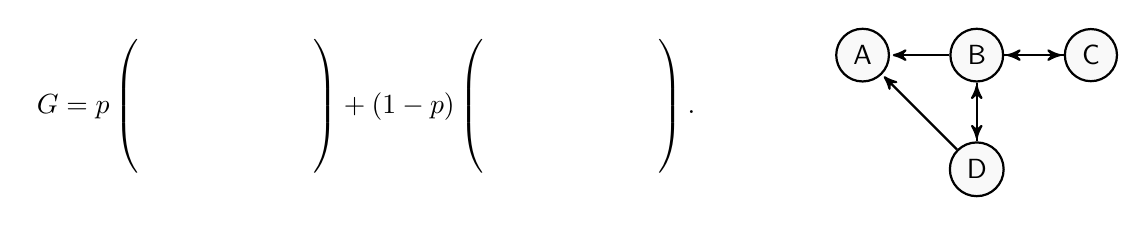
\begin{tikzpicture}
        \begin{scope}[->,>=stealth',shorten >=1pt,auto,node distance=1.45cm,thick, main node/.style={circle,fill=gray!05,draw}]
        \node[main node] (1) {A};
        \node[main node] (2) [right of=1] {B};
        \node[main node] (3) [below of=2] {D};
        \node[main node] (4) [right of=2] {C};
        \path[every node/.style={font=\sffamily\small}]
        (4) edge node[below] {} (2)
        (2) edge node [above] {} (1)
        edge [left] node {}  (3) 
        edge [left] node {}  (4) 
        (3) edge node {} (1)
        edge node[right] {} (2);
        %edge node[right] {} (5)
        %(4) edge node [above] {} (5)
        %(4) edge node [above] {} (5);
        \end{scope}
        \node[left] at (-2, -0.65) {$G = p\begin{pmatrix} &&&&&\\&\ &&&&\\&\ &&&&&\\&\ &&&&&\end{pmatrix} + (1-p)\begin{pmatrix} &&&&&\\&\ &&&&\\&\ &&&&&\\&\ &&&&&\end{pmatrix}.$};
    \end{tikzpicture}  
    \ifnum \Solutions=1 {\color{DarkBlue} \\ \textit{Solution:} The Google matrix is 
    $$G = p \begin{pmatrix} 
    1/4&1/3&0&1/2
    \\1/4&0&1&1/2
    \\1/4&1/3&0&0
    \\1/4&1/3&0&0 
    \end{pmatrix} + 
    (1-p)\begin{pmatrix}
    1/4&1/4&1/4&1/4\\
    1/4&1/4&1/4&1/4\\
    1/4&1/4&1/4&1/4\\
    1/4&1/4&1/4&1/4 
    \end{pmatrix}$$ 
    Note that we did not need to use the given value of $p$, which is ok. Also we could have written the answer (a bit) more neatly as: 
    $$G = p \begin{pmatrix} 
    1/4&1/3&0&1/2
    \\1/4&0&1&1/2
    \\1/4&1/3&0&0
    \\1/4&1/3&0&0 
    \end{pmatrix} + 
    \frac{(1-p)}{4}\begin{pmatrix}
    1&1&1&1\\
    1&1&1&1\\
    1&1&1&1\\
    1&1&1&1
    \end{pmatrix}$$     
    } \fi  
\fi 
\ifnum \Version=7 
    The steady-state probability vector for the Markov chain $\vec x_{k+1} = P\vec x_k$, where $k = 0,1,2,\ldots$ and $P=\dfrac15\begin{pmatrix} 3&1\\2&4\end{pmatrix}$ is $\vec q = \begin{pmatrix} c_1 \\c_2 \end{pmatrix}$, where $c_1 = \framebox{\strut\hspace{1cm}}$, $c_2 = \framebox{\strut\hspace{1cm}}$.
    \ifnum \Solutions=1 {\color{DarkBlue} \textit{Solution:} the steady state is a probability vector in the null space of $P-I$, and $$P-I = \begin{pmatrix} 3/5-1&1/5\\2/5&4/5-1 \end{pmatrix} \sim \begin{pmatrix} -2&1\\2&-1\end{pmatrix}$$ Then $\vec v = \begin{pmatrix} 1 & 2\end{pmatrix}^T$ is in the null space. But we need a probability vector. Dividing by the sum of the entries gives us the steady-state, $\vec q = \frac13 \begin{pmatrix} 1 & 2\end{pmatrix}^T$. So $c_1 = 1/3$, $c_2 = 2/3$. } \fi      
\fi 
\ifnum \Version=8
    $\lambda_1=3$ is an eigenvalue of $A$ with corresponding eigenvector $\vec v_1 = \begin{pmatrix} 5\\4\end{pmatrix}$. If $A\vec v_1 = \begin{pmatrix} c_1\\c_2\end{pmatrix}$, then $c_1 = \framebox{\strut\hspace{1cm}}$ and an eigenvalue of $A^2$ is \framebox{\strut\hspace{1cm}}. 
    
    \ifnum \Solutions=1 {\color{DarkBlue} \textit{Solution:} Since $\lambda_1$ is an eigenvalue of $A$, we must have that $$A\vec v_1 = \lambda_1 \vec v_1$$ Substituting the given information gives us $$A\vec v_1 = \lambda_1 \vec v_1 = 3 \begin{pmatrix} 5\\4 \end{pmatrix} = \begin{pmatrix} 15 \\ 12\end{pmatrix}$$  So $c_1 = 15$ and $c_2 = 12$. Moreover an eigenvalue of $A^2$ is 9. This is because we know that $A\vec v_1 = \lambda_1 \vec v_1$, so \begin{align}
        A\vec v_1 &= \lambda_1 \vec v_1 \\
        A(A\vec v_1) &= A(\lambda_1 \vec v_1) \\
        A^2\vec v_1 &= \lambda_1 A\vec v_1 \\
        A^2\vec v_1 &= \lambda_1^2 \vec v_1 
    \end{align}  } \fi    
\fi 
\ifnum \Version=9
    The area of the parallelogram with vertices at $(1,1)$, $(2,4)$, $(5,2)$, $(6,5)$ is \framebox{\strut\hspace{1cm}}. 
    \ifnum \Solutions=1 {\color{DarkBlue} \textit{Solution:} area is $\left| \det \begin{pmatrix} 1&4\\3&1\end{pmatrix} \right| = \left| 1\cdot1 - 3\cdot4 \right| = | 1 - 12 | = 12 - 1 = 11$. No credit for writing $-11$, as area cannot be negative. } \fi  
\fi 
\ifnum \Version=10
    If  $k$ is a  real number,  $A = \begin{pmatrix} 5&4\\k&k\end{pmatrix}$, $ B = \begin{pmatrix}15& k\\12 & k  \end{pmatrix}$, and $ \det A = 4$, then $\det B =  \framebox{\strut\hspace{1.2cm}}$ and $k= \framebox{\strut\hspace{1cm}}$.
    \ifnum \Solutions=1 {\color{DarkBlue} \textit{Solution:} matrix $B$ can be obtained from $A$ taking a transpose,  and multiplying a column by $3$. A transpose does not change the determinant.  Multiplying a column by $3$ multiplies the determinant by $3$. So $\det B = 12$. And if $\det A =4$, then \begin{align}
        \det A & = 4 \\
        \begin{vmatrix}
            5&4\\k&k 
        \end{vmatrix} &= 4 \\
        5k - 4k &= 4 \\
        k = 4
    \end{align}} \fi 
\fi 
\ifnum \Version=11
    $G$ is the Google Matrix for the set of four web pages that link to each other according to the diagram below. If the damping factor is $p=0.75$, fill in the missing entries of matrix $G$. 
    \vspace{4pt}
    
    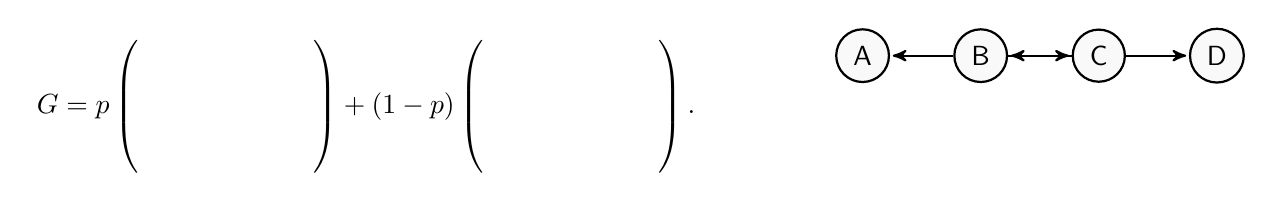
\begin{tikzpicture}
        \begin{scope}[->,>=stealth',shorten >=1pt,auto,node distance=1.5cm,thick, main node/.style={circle,fill=gray!05,draw}]
        \node[main node] (1) {A};
        \node[main node] (2) [right of=1] {B};
        \node[main node] (3) [right of=2] {C};
        \node[main node] (4) [right of=3] {D};
        \path[every node/.style={font=\sffamily\small}]
        (2) edge node [above] {} (1)
        edge [left] node {}  (3) 
        (3) edge node {} (2)
        edge node[right] {} (4);
        \end{scope}
        \node[left] at (-2, -0.65) {$G = p\begin{pmatrix} &&&&&\\&\ &&&&\\&\ &&&&&\\&\ &&&&&\end{pmatrix} + (1-p)\begin{pmatrix} &&&&&\\&\ &&&&\\&\ &&&&&\\&\ &&&&&\end{pmatrix}.$};
    \end{tikzpicture}  
    \ifnum \Solutions=1 {\color{DarkBlue} \\ \textit{Solution:} The Google matrix is 
    $$G = p \begin{pmatrix} 
    1/4&1/2&0&1/4\\
    1/4&0&1/2&1/4\\
    1/4&1/2&0&1/4\\
    1/4&0&1/2&1/4 
    \end{pmatrix} + 
    (1-p)\begin{pmatrix}
    1/4&1/4&1/4&1/4\\
    1/4&1/4&1/4&1/4\\
    1/4&1/4&1/4&1/4\\
    1/4&1/4&1/4&1/4 
    \end{pmatrix}$$ 
    Note that we did not need to use the given value of $p$, which is ok. Also we could have written the answer (a bit) more neatly as: 
    $$G = \frac p4 \begin{pmatrix} 
    1&2&0&1\\
    1&0&2&1\\
    1&2&0&1\\
    1&0&2&1 
    \end{pmatrix} + 
    \frac{(1-p)}{4}\begin{pmatrix}
    1&1&1&1\\
    1&1&1&1\\
    1&1&1&1\\
    1&1&1&1
    \end{pmatrix}$$     
    } \fi  
\fi 
\ifnum \Version=12
        Suppose that a $2\times 2$ matrix $A$ has eigenvalues $\lambda = 2$ and $\lambda= 3$. Then $\det(A^2) =  \framebox{\strut\hspace{1cm}}$. 
        \ifnum \Solutions=1 {\color{DarkBlue} \textit{Solution:} Using properties of determinants:
        \begin{align}
            \det(A^2) &= (\det A)^2 \\
            &= (\det (PDP^{-1}))^2 \\
            &= (\det P \det D \det P^{-1})^2\\
            &= (\det P  \det P^{-1} \det D)^2\\
            &= (\det (P P^{-1}) \det D)^4\\
            &= (\det (I) \det D)^2\\
            &= (\det D)^2
        \end{align}
        But $D$ is diagonal and its eigenvalues are 2 and 3, so $D$ is either 
        \begin{align}
            \begin{pmatrix} 3&0\\0&2\end{pmatrix} \quad \text{or} \quad \begin{pmatrix} 2&0\\0&3\end{pmatrix}
        \end{align}        
        Either way, $\det D = 3 \cdot 2 = 6$. So 
        \begin{align}
            \det(A^2) 
            &= (\det D)^2 = 6^2 = 36
        \end{align}        
        } \fi    
\fi 
\ifnum \Version=13 % 
    Let $S$ be an ellipse in whose area is 12. Then the area of $T(S)$, where $T(x) = Ax$, and $A = \begin{pmatrix} 2&4\\0&8\end{pmatrix}$ is \framebox{\strut\hspace{1cm}}.
    \ifnum \Solutions=1 {\color{DarkBlue} \textit{Solution:} The area of 
 is the area of the original ellipse 
, times the absolute value of the determinant of 
. We have
so area of 
 is   } \fi    
\fi 
\ifnum \Version=14 % 
    The steady-state vector of $P=\dfrac15\begin{pmatrix} 4&3\\1&2\end{pmatrix}$ is $\vec q = \begin{pmatrix} c_1 \\c_2 \end{pmatrix}$, where $c_1 = \framebox{\strut\hspace{1cm}}$, $c_2 = \framebox{\strut\hspace{1cm}}$.
        
    \ifnum \Solutions=1 {\color{DarkBlue} \textit{Solution:} the steady state is a probability vector in the null space of $P-I$, and $$P-I = \begin{pmatrix} 4/5-1&3/5\\1/5&2/5-1 \end{pmatrix} \sim \begin{pmatrix} -1&3\\1&-3\end{pmatrix}$$ Then $\begin{pmatrix} 3\\1\end{pmatrix}$ is in the null space. Dividing by the sum of the entries gives us the steady-state, $\vec q = \frac14 \begin{pmatrix} 3\\1\end{pmatrix}$. So $c_1 = 3/4, \ c_2 = 1/4$. } \fi   
\fi 
\ifnum \Version=15 % shouldn't need this version for fall 2023
    FILL IN THE BLANK ON UNIT 3
    \ifnum \Solutions=1 {\color{DarkBlue} \textit{Solution:} SOLUTION HERE  } \fi    
\fi 

\ifnum \Version=16 % shouldn't need this version for fall 2023
    FILL IN THE BLANK ON UNIT 3
    \ifnum \Solutions=1 {\color{DarkBlue} \textit{Solution:} SOLUTION HERE  } \fi    
\fi 

\ifnum \Version=17 % shouldn't need this version for fall 2023
    FILL IN THE BLANK ON UNIT 3
    \ifnum \Solutions=1 {\color{DarkBlue} \textit{Solution:} SOLUTION HERE  } \fi    
\fi 

\ifnum \Version=18 % shouldn't need this version for fall 2023
    FILL IN THE BLANK ON UNIT 3
    \ifnum \Solutions=1 {\color{DarkBlue} \textit{Solution:} SOLUTION HERE  } \fi    
\fi 




% \part Suppose $A$ is a $2\times 2$ matrix such that $\Nul A$ is the line $x_1-8x_2=0$, and a vector in $\Col A$ is $\vec u=\begin{pmatrix} 2\\4 \end{pmatrix}$. Then if $A=\begin{pmatrix}1 & c_1 \\ c_2 & c_3 \end{pmatrix} $, then $c_1= \framebox{\strut\hspace{1cm}}$, $c_2 =  \framebox{\strut\hspace{1cm}}$, and $c_3 =  \framebox{\strut\hspace{1cm}}$.

% \part If the LU factorization is $A=LU$, where $U$ is obtained by applying one row operation to $A$, and $A = \begin{pmatrix} 1&2&4\\3&2&12\end{pmatrix}$. Then $L = \begin{pmatrix} 1& 0\\l_1 & 1 \end{pmatrix} $ and $U= \begin{pmatrix} 1&2 & 4\\u_1 & u_2 & u_3 \end{pmatrix}$, where $l_1 = \framebox{\strut\hspace{1.25cm}}$, $u_1 = \framebox{\strut\hspace{1.25cm}}$, $u_2 = \framebox{\strut\hspace{1.25cm}}$ and $u_3 = \framebox{\strut\hspace{1.25cm}}$.

        
        % B) UNIT 1 BUT NOT TRANSFORMS

\ifnum \Version=1
    \part If $A= \begin{pmatrix} 2&1&0\\0&4&2\end{pmatrix}$ and $x=\begin{pmatrix} 1&h&k \end{pmatrix}^T$ is a solution to the homogeneous equation $Ax=0$, then $h=\framebox{\strut\hspace{1cm}}$ and $k=\framebox{\strut\hspace{1cm}}$.
    \ifnum \Solutions=1 {\color{DarkBlue} \textit{Solution:} Set $Ax=0$ and multiply $Ax$ to obtain two equations for the two unknowns $h$ and $k$. The equations are $$2+h=0, \ 4h + 2k = 0$$ Solving the equations gives us $h=-2$, $k=4$.  } \fi    
\fi 
\ifnum \Version=2
    \part Suppose the entries of $n\times n$ matrix $A$ are $a_{ij}$, and $n>2$. If $a_{ij} = 1$ when $i+j$ is even, and $a_{ij} = j$ when $i+j$ is odd, how many pivot columns would $A$ have? \framebox{\strut\hspace{1.25cm}} 
    
    \ifnum \Solutions=1 {\color{DarkBlue}

    For $n=3$ we have the matrix below.
    $$\begin{pmatrix} 1&2&1\\1&1&3\\1&2&1\end{pmatrix}$$
    The first and last rows are identical. If we reduce the matrix to echelon form there will be exactly two pivots. Likewise if $n=4$ we have
    $$
    \begin{pmatrix} 1&2&1&4\\1&1&3&1\\1&2&1&4\\1&1&3&1\end{pmatrix}
    $$
    The first and third rows are identical. And the second and fourth rows are identical. So if we reduce the matrix to echelon form there will be exactly two pivots again. Likewise if $n>4$ we always have exactly two pivots. So the answer to this question is two. 
    } 
   \fi    

\fi 
\ifnum \Version=3
    \part If $A$ is $42\times40$ and $A\vec x = \vec 0$ has exactly 2 free variables, how many pivots does $A$ have? \framebox{\strut\hspace{1cm}}
    \ifnum \Solutions=1 {\color{DarkBlue} \textit{Solution:} there are 40 columns and 2 of them are non-pivotal so there are 38 pivots.  } \fi       
\fi 
\ifnum \Version=4
    \part If $A=\begin{pmatrix} 2&8\\1&k\end{pmatrix}$ and $b = \begin{pmatrix} 3\\2\end{pmatrix}$, then $b$ is not in the span of the columns of $A$ when $k = \framebox{\strut\hspace{1cm}}$.
    \ifnum \Solutions=1 {\color{DarkBlue} \textit{Solution:} the columns have to be dependent which happens when $k=4$.  } \fi    
\fi 
\ifnum \Version=5
    \part Matrix $A$ is $2\times 2$, is in RREF, has linearly dependent columns, and every entry of $A$ is either 1 or 0. How many different matrices can you construct that meet all of these criteria? \framebox{\strut\hspace{1.25cm}}
    
    \ifnum \Solutions=1 {\color{DarkBlue} \textit{Solution:}  there are four such matrices: 
        $$\begin{pmatrix} 0&0\\0&0\end{pmatrix}
        , \begin{pmatrix} 1&0\\0&0\end{pmatrix}
        , \begin{pmatrix} 0&1\\0&0\end{pmatrix} 
        , \begin{pmatrix} 1&1\\0&0\end{pmatrix}
        $$ } \fi    
\fi 
\ifnum \Version=6
    \part If $A$ is $2 \times 3$ and is in RREF, and $\vec x = \begin{pmatrix} 12&4&-8\end{pmatrix}^T$ spans $\Null A$, then $A=\begin{pmatrix} a_1 & a_2 & a_3 \\ a_4 & a_5 & a_6 \end{pmatrix} $ where 
    $a_1 = \framebox{\strut\hspace{1.0cm}}$, 
    $a_2 = \framebox{\strut\hspace{1.0cm}}$, 
    $a_3 = \framebox{\strut\hspace{1.0cm}}$, 
    $a_4 = \framebox{\strut\hspace{1.0cm}}$,
    $a_5 = \framebox{\strut\hspace{1.0cm}}$,
    $a_6 = \framebox{\strut\hspace{1.0cm}}$.
    \ifnum \Solutions=1 {\color{DarkBlue} \textit{Solution:} If $x$ spans $\Null A$ then $A$ has two pivots. Since $A$ must also be in RREF we can set $a_1=a_5=1$ and $a_2=a_4 = 0$. So far we have
    $$A = \begin{pmatrix} 1&0&a_3\\0&1&a_6\end{pmatrix}$$
    But $A\vec x = \vec 0$, so 
    \begin{align}
        A\vec x = \begin{pmatrix} 1&0&a_3\\0&1&a_6\end{pmatrix}\begin{pmatrix} 12\\4\\-8\end{pmatrix} = \begin{pmatrix} 12-8a_3 \\4-8a_6 \end{pmatrix} = \begin{pmatrix} 0\\0 \end{pmatrix}
    \end{align}
    So $a_3 = 12/8=3/2$ and $a_6 = 4/8=1/2$. Listing all of the values:
    \begin{align}
        a_1 = 1, a_2 = 0, a_3 = 3/2, a_4=0, a_5 = 1, a_6 = 1/2
    \end{align} We would accept unsimplified fractions as correct. So for example $12/8$ is another correct answer for $a_3$.  } \fi    
\fi 
\ifnum \Version=7
    \part If the span of the columns of $A=\begin{pmatrix} 3&2\\9&k \end{pmatrix}$ is a line, then $k=\framebox{\strut\hspace{1cm}}$. 
    \ifnum \Solutions=1 {\color{DarkBlue} \textit{Solution:} $k=6$ because then the columns will be dependent and therefore will span a line instead of $\mathbb R^2$. } \fi      
\fi 
\ifnum \Version=8
    \part Matrix $A$ is $3\times 2$, is in echelon form, has linearly dependent columns, and every entry of $A$ is either 1 or 0. How many different matrices can you construct that meet all of these criteria? \framebox{\strut\hspace{1.25cm}}
    
    \ifnum \Solutions=1 {\color{DarkBlue} \textit{Solution:}  there are four such matrices: 
        $$\begin{pmatrix} 0&0\\0&0\\0&0\end{pmatrix}
        , \begin{pmatrix} 1&0\\0&0\\0&0\end{pmatrix}
        , \begin{pmatrix} 0&1\\0&0\\0&0\end{pmatrix} 
        , \begin{pmatrix} 1&1\\0&0\\0&0\end{pmatrix}
        $$ } \fi    
\fi 
\ifnum \Version=9
    \part If $A$ is $2 \times 3$ and is in RREF, and $\vec x = \begin{pmatrix} 12&6&-3\end{pmatrix}^T$ spans $\Null A$, then $A=\begin{pmatrix} a_1 & a_2 & a_3 \\ 0 & a_5 & a_6 \end{pmatrix} $ where 
    $a_1 = \framebox{\strut\hspace{1.0cm}}$, 
    $a_2 = \framebox{\strut\hspace{1.0cm}}$, 
    $a_3 = \framebox{\strut\hspace{1.0cm}}$, 
    $a_5 = \framebox{\strut\hspace{1.0cm}}$,
    $a_6 = \framebox{\strut\hspace{1.0cm}}$.
    \ifnum \Solutions=1 {\color{DarkBlue} \textit{Solution:} If $x$ spans $\Null A$ then $A$ has two pivots. Since $A$ must also be in RREF we can set $a_1=a_5=1$ and $a_2 = 0$. So far we have
    $$A = \begin{pmatrix} 1&0&a_3\\0&1&a_6\end{pmatrix}$$
    But $A\vec x = \vec 0$, so 
    \begin{align}
        A\vec x = \begin{pmatrix} 1&0&a_3\\0&1&a_6\end{pmatrix}\begin{pmatrix} 12\\6\\-3\end{pmatrix} = \begin{pmatrix} 12-3a_3 \\6-3a_6 \end{pmatrix} = \begin{pmatrix} 0\\0 \end{pmatrix}
    \end{align}
    So $a_3 = 12/3 = 4$ and $a_6 = 6/3 = 2$. Listing all of the values:
    \begin{align}
        a_1 = 1, a_2 = 0, a_3 = 4, a_4=0, a_5 = 1, a_6 = 2
    \end{align} We can accept un-simplified fractions as correct.   } \fi     
\fi 
\ifnum \Version=10
    \part If $A= \begin{pmatrix} 2&1&8\\0&1&-12\end{pmatrix}$ and $x=\begin{pmatrix} h&k&1 \end{pmatrix}^T$ is a solution to the homogeneous equation $Ax=0$, then $h=\framebox{\strut\hspace{1cm}}$ and $k=\framebox{\strut\hspace{1cm}}$.
    \ifnum \Solutions=1 {\color{DarkBlue} \textit{Solution:} solving $Ax = 0$ gives us the equations 
    \begin{align}
        2h + k + 8 &= 0 \\ k -12 &= 0
    \end{align}
    Solving this system gives us $h = -10 $, $k=12$.  } \fi     
\fi 
\ifnum \Version=11
    \part Matrix $A$ is $2\times 2$, is in echelon form, has linearly independent columns, and every entry of $A$ is either 1 or 0. How many different matrices can you construct that meet all of these criteria? \framebox{\strut\hspace{1.25cm}}

    \ifnum \Solutions=1 {\color{DarkBlue} \textit{Solutions.} 
    There are two such matrices: 
    $$\begin{pmatrix} 1&1\\0&1\end{pmatrix}
    , \begin{pmatrix} 1&0\\0&1\end{pmatrix}
    $$
    } 
    \fi
\fi 
\ifnum \Version=12
    \part Suppose the entries of $n\times n$ matrix $A$ are $a_{ij}$, and $n\ge2$. If $a_{ij} = 1$ when $i$ is even, and $a_{ij} = 2$ when $i$ is odd, how many pivot columns would $A$ have? \framebox{\strut\hspace{1.25cm}} 
    
    \ifnum \Solutions=1 {\color{DarkBlue}
    For $n=2$ we have the matrix below.
    $$\begin{pmatrix} 2&2\\1&1\end{pmatrix}$$
    For $n=3$ we have the matrix below.
    $$\begin{pmatrix} 2&2&2\\1&1&1\\2&2&2\end{pmatrix}$$
    The first and last rows are identical. If we reduce the matrix to echelon form there will be exactly one pivot. Likewise if $n=4$ we have
    $$\begin{pmatrix} 2&2&2&2\\1&1&1&1\\2&2&2&2\\1&1&1&1\end{pmatrix}$$
    The first and third rows are identical. And the second and fourth rows are identical. So if we reduce the matrix to echelon form there will be exactly one pivot again. Likewise if $n>4$ we always have exactly one pivot. So the answer to this question is one. 
    } 
   \fi    
\fi 
\ifnum \Version=13 % 
    \part If $A=\begin{pmatrix} 4&8\\1&k\end{pmatrix}$ and $b = \begin{pmatrix} 5\\2\end{pmatrix}$, then $b$ is not in the span of the columns of $A$ when $k = \framebox{\strut\hspace{1cm}}$.
    \ifnum \Solutions=1 {\color{DarkBlue} \textit{Solution:} the columns have to be dependent which happens when $k=2$.  } \fi   
\fi 
\ifnum \Version=14 % shouldn't need this version for fall 2023
    \part Matrix $A$ is $2\times 2$, is in RREF, and every entry of $A$ is either 1 or 0. How many different matrices can you construct that meet all of these criteria? \framebox{\strut\hspace{1.25cm}}

    \ifnum \Solutions=1 {\color{DarkBlue} \textit{Solutions.} 
    There are five such matrices: 
    $$\begin{pmatrix} 0&0\\0&0\end{pmatrix}
    , \begin{pmatrix} 1&0\\0&0\end{pmatrix}
    , \begin{pmatrix} 0&1\\0&0\end{pmatrix} 
    , \begin{pmatrix} 1&1\\0&0\end{pmatrix}
    , \begin{pmatrix} 1&0\\0&1\end{pmatrix}
    $$
    } 
    \fi
\fi 
\ifnum \Version=15 % shouldn't need this version for fall 2023
    \part FILL IN THE BLANK ON UNIT 1 BUT NOT TRANSFORMS
    \ifnum \Solutions=1 {\color{DarkBlue} \textit{Solution:} SOLUTION HERE  } \fi    
\fi 
\ifnum \Version=16 % shouldn't need this version for fall 2023
    \part FILL IN THE BLANK ON UNIT 1 BUT NOT TRANSFORMS
    \ifnum \Solutions=1 {\color{DarkBlue} \textit{Solution:} SOLUTION HERE  } \fi    
\fi 
\ifnum \Version=17 % shouldn't need this version for fall 2023
    \part FILL IN THE BLANK ON UNIT 1 BUT NOT TRANSFORMS
    \ifnum \Solutions=1 {\color{DarkBlue} \textit{Solution:} SOLUTION HERE  } \fi    
\fi 

        % F) UNIT 4
\part 
\ifnum \Version=1
    Suppose $A$ has the QR factorization $A=QR$, where $A = \begin{pmatrix} 0&6\\1&0\\0&8\end{pmatrix}, \ Q = \begin{pmatrix} 0&\frac35\\1&0\\0&\frac45\end{pmatrix}$. 
    Then $R=\begin{pmatrix} r_1&r_2\\r_3&r_4\end{pmatrix}$, where 
    $r_1=\framebox{\strut\hspace{1cm}}$, 
    $r_2=\framebox{\strut\hspace{1cm}}$, 
    $r_3=\framebox{\strut\hspace{1cm}}$, 
    $r_4=\framebox{\strut\hspace{1cm}}$.
    \ifnum \Solutions=1 {\color{DarkBlue} \textit{Solution:} $R=Q^TA = \begin{pmatrix} 1&0\\0&10 \end{pmatrix}.$  } \fi    
\fi 
\ifnum \Version=2
    Vectors $u_1$ and $u_2$ form an orthogonal set. The projection of $y$ onto $S=\Span\{u_1,u_2\}$ is $\hat y = \proj_Sy$, where $y_1=\framebox{\strut\hspace{1cm}}$, 
    $y_2=\framebox{\strut\hspace{1cm}}$, $y_3=\framebox{\strut\hspace{1cm}}$. $$u_1 = \begin{pmatrix} 1\\2\\1\end{pmatrix}, \quad u_2 = \begin{pmatrix} 2\\-1\\0\end{pmatrix}, \quad y = \begin{pmatrix} 1\\0\\-1\end{pmatrix}, \quad \hat y = \begin{pmatrix} y_1\\y_2\\y_3\end{pmatrix}$$
    \ifnum \Solutions=1 {\color{DarkBlue} \textit{Solution:} the usual procedure yields
    \begin{align}
        \hat y &= \frac{y\cdot u_1}{u_1 \cdot u_1}u_1 + \frac{y\cdot u_2}{u_2 \cdot u_2}u_2 
        = 0 + \frac{2}{5}u_2
        = \begin{pmatrix} 4/5\\-2/5\\ 0\end{pmatrix} 
    \end{align}
    So $y_1=4/5, y_2=-2/5, y_3=0$. There are no other possible solutions.}
    \fi    
\fi 
\ifnum \Version=3
    An orthogonal basis for the subspace $S = \Span (y_1, y_2)$ is given by the set of vectors $\{\hat y_1, \hat y_2\}$, where $y_1 = \hat y_1$, $x_1 = \framebox{\strut\hspace{1cm}}$, $x_2 = \framebox{\strut\hspace{1cm}}$, and 
    $$
    y_1 = \hat y_1 = \begin{pmatrix} 2\\-5\\1\end{pmatrix}, \quad 
    y_2 = \begin{pmatrix} 8\\-2\\4\end{pmatrix}, \quad 
    \hat y_2 = \begin{pmatrix} x_1\\x_2\\ 3 \end{pmatrix}, \quad 
    $$
    
    \ifnum \Solutions=1 {\color{DarkBlue} \textit{Solution:} the usual procedure yields
    \begin{align}
        \hat y_2 
        &= y_2 - \frac{y_2\cdot y_1}{y_1 \cdot y_1}y_1 
        = \begin{pmatrix} 8\\-2\\4\end{pmatrix} - \frac{30}{30}\begin{pmatrix} 2\\-5\\1\end{pmatrix} 
        = \begin{pmatrix} 6\\3\\3\end{pmatrix}
    \end{align}
    So $x_1=6, x_2=3$. 
    } \fi    
\fi 
\ifnum \Version=4
    Vectors $u_1$ and $u_2$ form an orthogonal set. The projection of $y$ onto $S=\Span\{u_1,u_2\}$ is $\hat y = \proj_Sy$, where $y_1=\framebox{\strut\hspace{1cm}}$, 
    $y_2=\framebox{\strut\hspace{1cm}}$. $$u_1 = \begin{pmatrix} 1\\2\\2\end{pmatrix}, \quad u_2 = \begin{pmatrix} 2\\-1\\0\end{pmatrix}, \quad y = \begin{pmatrix} 1\\2\\11\end{pmatrix}, \quad \hat y = \begin{pmatrix} y_1\\y_2\\y_3\end{pmatrix}$$
    \ifnum \Solutions=1 {\color{DarkBlue} \textit{Solution:} the usual process yields
    \begin{align}
        \hat y &= \frac{y\cdot u_1}{u_1 \cdot u_1}u_1 + \frac{y\cdot u_2}{u_2 \cdot u_2}u_2 
        = \frac{27}{9}u_1 + 0u_2 = 3u_1 
        = \begin{pmatrix} 3\\6\\ 6\end{pmatrix} 
    \end{align}
    So $y_1=3, y_2=6, y_3=6$. There are no other possible solutions. } \fi  
\fi 
\ifnum \Version=5
    If matrix $A$ is $20\times 25$ and dim($(\Col A)\Perp$) = 5, the rank of $A$ is \framebox{\strut\hspace{1cm}}.
    \ifnum \Solutions=1 {\color{DarkBlue} \textit{Solution:} The answer is 15, because we are told that $5 = \dim ((\Col A)\Perp) = \dim(\Null (A^T))$. So $A^T$ has 5 non-pivotal columns, which means that $A$ has 5 non-pivotal rows. $A$ has 20 rows, so 15 rows are pivotal. And $\text{rank} A = \text{number of pivotal columns} = \text{number of pivotal rows} = 15$.   } \fi    
\fi 
\ifnum \Version=6
    The distance between $u=\begin{pmatrix} 5\\4\end{pmatrix}$ and the subspace $W=\text{Span}(v)$, where $v = \begin{pmatrix} 0\\1\end{pmatrix}$, is \framebox{\strut\hspace{1cm}}.     
    \ifnum \Solutions=1 {\color{DarkBlue} \textit{Solution:} 5. You might want to try sketching $u$ and the span of $v$ to see why the answer is 5.   } \fi    
\fi 
\ifnum \Version=7 
    Vectors $u_1$ and $u_2$ form an orthogonal set. The projection of $y$ onto $S=\Span\{u_1,u_2\}$ is $\hat y = \proj_Sy$, where $y_1=\framebox{\strut\hspace{1cm}}$, 
    $y_2=\framebox{\strut\hspace{1cm}}$. 
    $$
    u_1 = \begin{pmatrix} 3\\1\\0\end{pmatrix}, \quad 
    u_2 = \begin{pmatrix} 1\\-3\\2\end{pmatrix}, \quad 
    y = \begin{pmatrix} -1\\3\\12\end{pmatrix}, \quad 
    \hat y = \begin{pmatrix} y_1\\y_2\\y_3\end{pmatrix}
    $$
    \ifnum \Solutions=1 {\color{DarkBlue} \textit{Solution:} the usual process yields
    \begin{align}
        \hat y &= \frac{y\cdot u_1}{u_1 \cdot u_1}u_1 + \frac{y\cdot u_2}{u_2 \cdot u_2}u_2 
        = 0u_1 + \frac{14}{14}u_2 = u_2 
        = \begin{pmatrix} 1\\-3\\2\end{pmatrix} 
    \end{align}
    So $y_1=1, y_2=-3, y_3=2$. There are no other possible solutions. } \fi  
\fi 
\ifnum \Version=8
    The distance between $u=\begin{pmatrix} 3\\4\end{pmatrix}$ and the subspace $W=\text{Span}(v)$, where $v = \begin{pmatrix} 4\\-3\end{pmatrix}$, is \framebox{\strut\hspace{1cm}}.     
    \ifnum \Solutions=1 {\color{DarkBlue} \textit{Solution:} The distance is 5. Because the distance is given by $$\| y - \proj _W u \| = \| y - \frac{u\cdot v}{v\cdot v}v \| = \| y - 0 \| = \|y \| = 5$$.   } \fi    
\fi 
\ifnum \Version=9
    Vectors $u_1$ and $u_2$ form an orthogonal set. The projection of $y$ onto $S=\Span\{u_1,u_2\}$ is $\hat y = \proj_Sy$, where $y_1=\framebox{\strut\hspace{1cm}}$, 
    $y_2=\framebox{\strut\hspace{1cm}}$. $$u_1 = \begin{pmatrix} 1\\3\\2\end{pmatrix}, \quad u_2 = \begin{pmatrix} 3\\-1\\0\end{pmatrix}, \quad y = \begin{pmatrix} 4\\2\\2\end{pmatrix}, \quad \hat y = \begin{pmatrix} y_1\\y_2\\y_3\end{pmatrix}$$
    \ifnum \Solutions=1 {\color{DarkBlue} \textit{Solution:} the usual process yields
    \begin{align}
        \hat y &= \frac{y\cdot u_1}{u_1 \cdot u_1}u_1 + \frac{y\cdot u_2}{u_2 \cdot u_2}u_2 
        = \frac{14}{14}u_1 + \frac{10}{10}u_2 = u_1 + u_2 = \begin{pmatrix} 4\\2\\2\end{pmatrix}
    \end{align}
    So $y_1=4, y_2=2, y_3=2$. There are no other possible solutions. } \fi    
\fi 
\ifnum \Version=10
    Matrix $A = \begin{pmatrix} 0\\2\end{pmatrix}$ has the QR factorization $A = QR$, where $Q = \begin{pmatrix} q_1\\q_2\end{pmatrix}$, $R = r_1$, and 
    $q_1 = \framebox{\strut\hspace{1cm}}$, 
    $q_2 = \framebox{\strut\hspace{1cm}}$, 
    $r_1 = \framebox{\strut\hspace{1cm}}$.
    \ifnum \Solutions=1 {\color{DarkBlue} \textit{Solution:} the columns of $Q$ are an orthonormal basis for $\Col A$, so we can use $Q = \begin{pmatrix} 0\\1\end{pmatrix}$ or $Q = \begin{pmatrix} 0\\-1\end{pmatrix}$. And $R$ can be found using $R=Q^TA$. So 
    \begin{align}
        R = Q^TA = \begin{pmatrix} 0 & 1 \end{pmatrix}\begin{pmatrix} 0\\2\end{pmatrix} = 0 + 2 = 2
    \end{align} But we defined $R$ in such a way so that the entries on the main diagonal must be positive, so we can't use $Q = \begin{pmatrix} 0\\-1\end{pmatrix}$. So the only possible answer to this question is $q_1 = 0$, $q_2 = 1$, $r_1 = 2$.
    }\fi    
\fi 
\ifnum \Version=11
    Suppose $A$ has the QR factorization $A=QR$, where $A = \begin{pmatrix} 0&6\\1&0\\0&8\end{pmatrix}$. Then $Q = \begin{pmatrix} 0&3/5\\1&0\\0&4/5\end{pmatrix}$ and $R=\begin{pmatrix} r_1&r_2\\r_3&r_4\end{pmatrix}$, where 
    $r_1=\framebox{\strut\hspace{1cm}}$, 
    $r_2=\framebox{\strut\hspace{1cm}}$, 
    $r_3=\framebox{\strut\hspace{1cm}}$, 
    $r_4=\framebox{\strut\hspace{1cm}}$.
    
    \ifnum \Solutions=1 {\color{DarkBlue} We can use $R=Q^TA$. Performing the matrix multiplication:
    \begin{align}Q^TA &=  \begin{pmatrix} 0&1&0\\3/5&0&4/5\end{pmatrix} \begin{pmatrix} 0&6\\1&0\\0&8\end{pmatrix} \\
    &=  \begin{pmatrix} 0*0 + 1*1 + 0*0 & 0 \\ 0 & 3/5*6 + 0*0 + 4/5*8 \end{pmatrix} \\
    &= \begin{pmatrix} 1 & 0 \\ 0 & \frac{18+32}{5} \end{pmatrix} \\
    &= \begin{pmatrix} 1 & 0 \\ 0 & \frac{50}{5} \end{pmatrix} 
    \end{align}
    So $r_1 = 1$, $r_2=r_3=0$, $r_4=10$. Un-simplified fractions are acceptable. } \fi 
\fi 
\ifnum \Version=12
    Vectors $u_1$ and $u_2$ are an orthogonal basis for $S=\Span\{u_1,u_2\}$. The projection of $y$ onto $S$ is $\hat y = \proj_Sy$, where $y_1=\framebox{\strut\hspace{1cm}}$, 
    $y_2=\framebox{\strut\hspace{1cm}}$, $y_3 = \framebox{\strut\hspace{1cm}}$. $$u_1 = \begin{pmatrix} 2\\-4\\1\end{pmatrix}, \quad u_2 = \begin{pmatrix} 2\\1\\0\end{pmatrix}, \quad y = \begin{pmatrix} 4\\2\\21\end{pmatrix}, \quad \hat y = \begin{pmatrix} y_1\\y_2\\y_3\end{pmatrix}$$
    \ifnum \Solutions=1 {\color{DarkBlue} \textit{Solution:} the usual process yields
    \begin{align}
        \hat y 
        &= \frac{y\cdot u_1}{u_1 \cdot u_1}u_1 + \frac{y\cdot u_2}{u_2 \cdot u_2}u_2 
        = \frac{21}{21}u_1 + \frac{10}{5}u_2 = u_1 + 2u_2 
        =  \begin{pmatrix} 2\\-4\\1\end{pmatrix} + \begin{pmatrix} 4\\2\\0\end{pmatrix} 
        = \begin{pmatrix} 6\\-2\\1\end{pmatrix}
    \end{align}
    So $y_1=6, y_2=-2, y_3=1$. There are no other possible solutions. } \fi    
\fi 
\ifnum \Version=13
    An orthogonal basis for the subspace $S = \Span (y_1, y_2)$ is given by the set of vectors $\{\hat y_1, \hat y_2\}$, where $y_1 = \hat y_1$, $x_1 = \framebox{\strut\hspace{1cm}}$, $x_2 = \framebox{\strut\hspace{1cm}}$, and 
    $$
    y_1 = \hat y_1 = \begin{pmatrix} 2\\-5\\1\end{pmatrix}, \quad 
    y_2 = \begin{pmatrix} 8\\-2\\4\end{pmatrix}, \quad 
    \hat y_2 = \begin{pmatrix} x_1\\x_2\\ 3 \end{pmatrix}, \quad 
    $$
    
    \ifnum \Solutions=1 {\color{DarkBlue} \textit{Solution:} the usual procedure yields
    \begin{align}
        \hat y_2 
        &= y_2 - \frac{y_2\cdot y_1}{y_1 \cdot y_1}y_1 
        = \begin{pmatrix} 8\\-2\\4\end{pmatrix} - \frac{30}{30}\begin{pmatrix} 2\\-5\\1\end{pmatrix} 
        = \begin{pmatrix} 6\\3\\3\end{pmatrix}
    \end{align}
    So $x_1=6, x_2=3$. 
    } \fi    
\fi 
\ifnum \Version=14 % 
    Suppose $A$ has the QR factorization $A=QR$, where $A = \begin{pmatrix} 0&5\\1&0\\0&12\end{pmatrix}, \ Q = \begin{pmatrix} 0&\frac{5}{13}\\1&0\\0&\frac{12}{13}\end{pmatrix}$. 
    Then $R=\begin{pmatrix} r_1&r_2\\r_3&r_4\end{pmatrix}$, where 
    $r_1=\framebox{\strut\hspace{1cm}}$, 
    $r_2=\framebox{\strut\hspace{1cm}}$, 
    $r_3=\framebox{\strut\hspace{1cm}}$, 
    $r_4=\framebox{\strut\hspace{1cm}}$.
    \ifnum \Solutions=1 {\color{DarkBlue} \textit{Solution:} $R=Q^TA = \begin{pmatrix} 1&0\\0&13 \end{pmatrix}.$ So $r_1 = 1$, $r_2=r_3=0$, $r_4=13$.  } \fi    
\fi 
\ifnum \Version=15 % shouldn't need this version for fall 2023
    FILL IN THE BLANK ON UNIT 4
    \ifnum \Solutions=1 {\color{DarkBlue} \textit{Solution:} SOLUTION HERE  } \fi    
\fi 
\ifnum \Version=16 % shouldn't need this version for fall 2023
    FILL IN THE BLANK ON UNIT 4
    \ifnum \Solutions=1 {\color{DarkBlue} \textit{Solution:} SOLUTION HERE  } \fi    
\fi 
\ifnum \Version=17 % shouldn't need this version for fall 2023
    FILL IN THE BLANK ON UNIT 4
    \ifnum \Solutions=1 {\color{DarkBlue} \textit{Solution:} SOLUTION HERE  } \fi    
\fi 
\ifnum \Version=18 % shouldn't need this version for fall 2023
    FILL IN THE BLANK ON UNIT 4
    \ifnum \Solutions=1 {\color{DarkBlue} \textit{Solution:} SOLUTION HERE  } \fi    
\fi 

        % C) U2

\ifnum \Version=1
    \part The LU factorization of $A = \begin{pmatrix} 2&5\\4&12\end{pmatrix}$ is $A=LU$, where $U$ is obtained by applying only one row operation to $A$. Then $U=\begin{pmatrix} 2&5\\u_1&u_2\end{pmatrix}$ and $L=\begin{pmatrix} l_1& 0\\l_2&l_3 \end{pmatrix}$, where 
    $u_1 = \framebox{\strut\hspace{1.00cm}}$, 
    $u_2 = \framebox{\strut\hspace{1.00cm}}$, 
    $l_1 = \framebox{\strut\hspace{1.00cm}}$, 
    $l_2 = \framebox{\strut\hspace{1.00cm}}$, and
    $l_3 = \framebox{\strut\hspace{1.00cm}}$. 
    \ifnum \Solutions=1 {\color{DarkBlue} \textit{Solution:} the only correct answer is $U=\begin{pmatrix} 2&5\\0&2 \end{pmatrix}$ and $L=\begin{pmatrix} 1&0\\2&1\end{pmatrix}$. } \fi 
\fi 

\ifnum \Version=2
    \part Suppose that we want reflect points in $\mathbb R^2$ across the line $x_1 = 4$. Using homogeneous coordinates we can use a transform of the form $T(\vec x) = A\vec x$, where $\vec x \in \mathbb R^3$ and $A$ is $$A = \begin{pmatrix} 1&0&a_1\\0&1&a_2\\0&0&a_3\end{pmatrix}\begin{pmatrix}b_1&b_2&0\\b_3&b_4&0\\0&0&1 \end{pmatrix}\begin{pmatrix} 1&0&c_1\\0&1&c_2\\0&0&c_3 \end{pmatrix}$$ Then $a_1 = \framebox{\strut\hspace{1.0cm}}$, $a_2 = \framebox{\strut\hspace{1.0cm}}$, $b_1 = \framebox{\strut\hspace{1.0cm}}$, $b_2 = \framebox{\strut\hspace{1.0cm}}$, $c_1 = \framebox{\strut\hspace{1.0cm}}$, $c_2 = \framebox{\strut\hspace{1.0cm}}$.
    \ifnum \Solutions=1 {\color{DarkBlue} \textit{Solutions.} 
    The matrices we need are
    $$A = \begin{pmatrix} 1&0&4\\0&1&0\\0&0&1\end{pmatrix}\begin{pmatrix}-1&0&0\\0&1&0\\0&0&1 \end{pmatrix}\begin{pmatrix} 1&0&-4\\0&1&0\\0&0&1 \end{pmatrix}$$    
    So $a_1 = 4, a_2 = 0, b_1 = -1, b_2 = 0, c_1 = -4, c_2 = 0$. 
    } 
    \fi    
\fi 
\ifnum \Version=3
    \part If $A = \begin{pmatrix} 1& 0 & 2 \\4&1&0\\0&0&1\end{pmatrix}$, then $A^{-1} = \begin{pmatrix} 1&0&c_1\\c_2&1&c_3\\0&0&1\end{pmatrix}$, where $c_1 = \framebox{\strut\hspace{.75cm}}$, $ c_2 = \framebox{\strut\hspace{.75cm}}$, $c_3 = \framebox{\strut\hspace{.75cm}}$. 
    \ifnum \Solutions=1 {\color{DarkBlue} \\[12pt] 
        There are a few ways to determine the values of the $c$'s. Here are a few methods. 
        \begin{itemize}
            \item Forming the augmented matrix $\begin{pmatrix}A \ | \ I\end{pmatrix}$ and reducing yields:
        \begin{align*}
            \begin{pmatrix}A \ | \ I\end{pmatrix} 
            = \begin{pmatrix} 1& 0 & 2 &1&0&0\\4&1&0&0&1&0\\0&0&1&0&0&1\end{pmatrix} 
            &\sim \begin{pmatrix} 1& 0 & 2 &1&0&0\\0&1&-8&-4&1&0\\0&0&1&0&0&1\end{pmatrix}\\
            &\sim \begin{pmatrix} 1& 0 & 2 &1&0&0\\0&1&0&-4&1&8\\0&0&1&0&0&1\end{pmatrix} \\
            &\sim \begin{pmatrix} 1& 0 & 0 &1&0&-2\\0&1&0&-4&1&8\\0&0&1&0&0&1\end{pmatrix}  = \begin{pmatrix}I \ | \ A^{-1}\end{pmatrix} 
        \end{align*}
        So $A^{-1} = \begin{pmatrix} 1&0&-2\\-4&1&8\\0&0&1\end{pmatrix}$ and $c_1 = -2, c_2 = -4, c_3 = 8$. 
        \item We could also set $AA^{-1} = I$ and solve for the unknowns. 
        \begin{align}
            AA^{-1} = \begin{pmatrix} 1& 0 & 2 \\4&1&0\\0&0&1\end{pmatrix}\begin{pmatrix} 1&0&c_1\\c_2&1&c_3\\0&0&1\end{pmatrix}
            &= \begin{pmatrix} 1&0&c_1+2\\4+c_2&1&4c_1+c_3\\0&0&1\end{pmatrix}
        \end{align}
        But $AA^{-1} = I$, so we have the equations
        \begin{align}
            c_1+2 &=0 \\
            4+c_2 &=0 \\
            4c_1 +c_3 &= 0
        \end{align}
        Solving these equations also gives us $c_1 = -2, c_2 = -4, c_3 = 8$.
        \end{itemize}
    } 
    \fi
\fi 
\ifnum \Version=4
    % Version 4 has a graphing question so skip 
\fi 
\ifnum \Version=5
    \part Suppose $A$, $B$, $C$ and $D$ are invertible $n\times n$ matrices, and $X= \begin{pmatrix} A & B\end{pmatrix}$, and $Y = \begin{pmatrix} C & D\end{pmatrix}$. If $XY^T=2AC^T$, then $D = \framebox{\strut\hspace{2cm}}$
    
    \ifnum \Solutions=1 {\color{DarkBlue} \textit{Solution:}  \begin{align}
        XY^T = \begin{pmatrix} A & B\end{pmatrix}\begin{pmatrix} C^T \\ D^T \end{pmatrix} & = 2AC^T\\
        AC^T + BD^T &= 2AC^T \\
        BD^T &= AC^T \\
        D^T &= B^{-1} AC^T \\
        D &= (B^{-1} AC^T)^T
    \end{align} It would also be ok to leave the answer as $D = CA^T(B^{-1})^T$.} \fi    
\fi 
\ifnum \Version=6
    \part If $A$ has LU factorization $A=LU$, where $U = \begin{pmatrix} 2&1\\0&3\end{pmatrix}$, and the solution to $L\vec y = \begin{pmatrix}6\\12 \end{pmatrix}$ is $\vec y = \begin{pmatrix} 2\\24 \end{pmatrix}$, then the solution to $A\vec x = \begin{pmatrix}6\\12 \end{pmatrix}$ is $\vec x = \begin{pmatrix} x_1\\x_2\end{pmatrix}$, where $x_1 = \framebox{\strut\hspace{1.0cm}}$, $x_2 = \framebox{\strut\hspace{1.0cm}}$.
    \ifnum \Solutions=1 {\color{DarkBlue} \textit{Solutions.} 
    If $A\vec x = LU\vec x = \begin{pmatrix} 6\\12 \end{pmatrix}$, and $L\vec y = \begin{pmatrix} 6\\12 \end{pmatrix}$ then $U\vec x = \vec y$. But we are given $\vec y$, so \begin{align} U\vec x = \begin{pmatrix} 2\\24 \end{pmatrix}\end{align} Expressing this as an augmented matrix we obtain 
    $$\begin{pmatrix} 2&1 & 2\\0&3&24 \end{pmatrix} \sim \begin{pmatrix} 2&1&2\\0&1&8\end{pmatrix} \sim \begin{pmatrix} 1&0&-3\\0&1&8\end{pmatrix}$$
    Thus $x_1 = -3$, $x_2= 8$. }
\fi
\fi 
\ifnum \Version=7
    \part The LU factorization of $A = \begin{pmatrix} 2&5\\4&12\end{pmatrix}$ is $A=LU$, where $U$ is obtained by applying only one row operation to $A$. Then $U=\begin{pmatrix} 2&5\\u_1&u_2\end{pmatrix}$ and $L=\begin{pmatrix} l_1& 0\\l_2&l_3 \end{pmatrix}$, where 
    $u_1 = \framebox{\strut\hspace{1.00cm}}$, 
    $u_2 = \framebox{\strut\hspace{1.00cm}}$, 
    $l_1 = \framebox{\strut\hspace{1.00cm}}$, 
    $l_2 = \framebox{\strut\hspace{1.00cm}}$, and
    $l_3 = \framebox{\strut\hspace{1.00cm}}$. 
    \ifnum \Solutions=1 {\color{DarkBlue} \textit{Solution:} the only correct answer is $U=\begin{pmatrix} 2&5\\0&2 \end{pmatrix}$ and $L=\begin{pmatrix} 1&0\\2&1\end{pmatrix}$. } \fi  
\fi 
\ifnum \Version=8
    \part If $A = \begin{pmatrix} 1& 0 & 3 \\4&1&0\\0&0&1\end{pmatrix}$, then $A^{-1} = \begin{pmatrix} 1&0&c_1\\c_2&1&c_3\\0&0&1\end{pmatrix}$, where $c_1 = \framebox{\strut\hspace{.75cm}}$, $ c_2 = \framebox{\strut\hspace{.75cm}}$, $c_3 = \framebox{\strut\hspace{.75cm}}$. 
    \ifnum \Solutions=1 {\color{DarkBlue} \\[12pt] 
        There are a few ways to determine the values of the $c$'s. Here are a few methods. 
        \begin{itemize}
            \item Forming the augmented matrix $\begin{pmatrix}A \ | \ I\end{pmatrix}$ and reducing yields:
        \begin{align*}
            \begin{pmatrix}A \ | \ I\end{pmatrix} 
            = \begin{pmatrix} 1& 0 & 3 &1&0&0\\4&1&0&0&1&0\\0&0&1&0&0&1\end{pmatrix} 
            &\sim \begin{pmatrix} 1& 0 & 3 &1&0&0\\0&1&-12&-4&1&0\\0&0&1&0&0&1\end{pmatrix}\\
            &\sim \begin{pmatrix} 1& 0 & 3 &1&0&0\\0&1&0&-4&1&12\\0&0&1&0&0&1\end{pmatrix} \\
            &\sim \begin{pmatrix} 1& 0 & 0 &1&0&-3\\0&1&0&-4&1&12j\\0&0&1&0&0&1\end{pmatrix}  = \begin{pmatrix}I \ | \ A^{-1}\end{pmatrix} 
        \end{align*}
        So $A^{-1} = \begin{pmatrix} 1&0&-3\\-4&1&8\\0&0&1\end{pmatrix}$ and $c_1 = -3, c_2 = -4, c_3 = 12$. 
        \item We could also set $AA^{-1} = I$ (or $A^{-1}A = I$), then multiply the matrices together, and then solve for the unknowns. The process should give the same values. 
        \end{itemize}
    } 
    \fi
\fi 
\ifnum \Version=9
    \part Determine all possible values of $k$ so that $AB=BA$, where $A = \begin{pmatrix} 2&k\\0&1\end{pmatrix}$ and $B = \begin{pmatrix} 1&-3\\0&2\end{pmatrix}$. $k = \framebox{\strut\hspace{1cm}}$. 
    \ifnum \Solutions=1 {\color{DarkBlue} \textit{Solution:} To determine all possible values of \(k\) such that \(AB = BA\) we can compute the products \(AB\) and \(BA\) and then set them equal to each other.
    \[ AB = \begin{pmatrix} 2 & k \\ 0 & 1 \end{pmatrix} \begin{pmatrix} 1 & -3 \\ 0 & 2 \end{pmatrix} =  \begin{pmatrix} 2 & -6 + 2k \\ 0 & 2 \end{pmatrix}.\]

    The product \(BA\) is:
    \[ BA = \begin{pmatrix} 1 & -3 \\ 0 & 2 \end{pmatrix} \begin{pmatrix} 2 & k \\ 0 & 1 \end{pmatrix} = \begin{pmatrix} 2 & k - 3 \\ 0 & 2 \end{pmatrix}.\]
    Now, we set \(AB = BA\) and compare the corresponding entries:
    \[ \begin{pmatrix} 2 & -6 + 2k \\ 0 & 2 \end{pmatrix} = \begin{pmatrix} 2 & k - 3 \\ 0 & 2 \end{pmatrix}.\]
    This leads to the following:
    \begin{align*}
    -6 + 2k &= k - 3, \\
    k & = 3
    \end{align*} 
     The only possible value of \(k\) is \(\boxed{3}\).
    } \fi    
\fi 
\ifnum \Version=10
    \part Suppose that we want reflect points in $\mathbb R^2$ across the line $x_2 = -3$. Using homogeneous coordinates we can use a transform of the form $T(\vec x) = A\vec x$, where $\vec x \in \mathbb R^3$ and $A$ is the matrix $$A = \begin{pmatrix} 1&0&a_1\\0&1&a_2\\0&0&a_3\end{pmatrix}\begin{pmatrix}b_1&b_2&0\\b_3&b_4&0\\0&0&1 \end{pmatrix}\begin{pmatrix} 1&0&c_1\\0&1&c_2\\0&0&c_3 \end{pmatrix}$$ Then 
    $a_1 = \framebox{\strut\hspace{1.00cm}}$, 
    $a_2 = \framebox{\strut\hspace{1.00cm}}$, 
    $b_1 = \framebox{\strut\hspace{1.00cm}}$, 
    $b_2 = \framebox{\strut\hspace{1.00cm}}$, 
    $c_1 = \framebox{\strut\hspace{1.00cm}}$, and 
    $c_2 = \framebox{\strut\hspace{1.00cm}}$.
    \ifnum \Solutions=1 {\color{DarkBlue} \textit{Solutions.} 
    The matrices we need are
    $$A = 
    \begin{pmatrix} 1&0&0\\0&1&-3\\0&0&1\end{pmatrix}
    \begin{pmatrix}1&0&0\\0&-1&0\\0&0&1 \end{pmatrix}
    \begin{pmatrix} 1&0&0\\0&1&3\\0&0&1 \end{pmatrix}$$    
    So $a_1 = 0, a_2 = -3, b_1 = 1, b_2 = 0, c_1 = 0, c_2 = 3$. 
    } 
    \fi       
\fi 
\ifnum \Version=11
    % no question needed here - will have a question 6
\fi 
\ifnum \Version=12
    % no question needed here - will have a question 6
\fi 
\ifnum \Version=13 % make-up
        % No problem needed because this version has a graphing problem 
\fi 
\ifnum \Version=14 % 
    \ifnum \Solutions=1 \newpage \fi
    \part If $A = \begin{pmatrix} 1& 0 & 0 \\4&1&0\\0&5&1\end{pmatrix}$, then $A^{-1} = \begin{pmatrix} 1&0&0\\c_1&1&0\\c_2&c_3&1\end{pmatrix}$, where $c_1 = \framebox{\strut\hspace{.75cm}}$, $ c_2 = \framebox{\strut\hspace{.75cm}}$, $c_3 = \framebox{\strut\hspace{.75cm}}$. 
    \ifnum \Solutions=1 {\color{DarkBlue} \\[12pt] 
        There are a few ways to determine the values of the $c$'s. Here are a few methods. 
        \begin{itemize}
            \item Forming the augmented matrix $\begin{pmatrix}A \ | \ I\end{pmatrix}$ and reducing yields:
        \begin{align*}
            \begin{pmatrix}A \ | \ I\end{pmatrix} 
            &= \begin{pmatrix} 1& 0 & 0 &1&0&0\\4&1&0&0&1&0\\0&5&1&0&0&1\end{pmatrix} \\
            &\sim \begin{pmatrix} 1& 0 & 0 &1&0&0\\0&1&0&-4&1&0\\0&5&1&0&0&1\end{pmatrix} \\
            &\sim \begin{pmatrix} 1& 0 & 0 &1&0&0\\0&1&0&-4&1&0\\0&5&1&20&-5&1\end{pmatrix} 
            = \begin{pmatrix}I \ | \ A^{-1}\end{pmatrix} 
        \end{align*}
        So $A^{-1} = \begin{pmatrix} 1&0&0\\-4&1&0\\20&-5&1\end{pmatrix}$ and $c_1 = -4, c_2 = 20, c_3 = -5$. 
        \item We could also set $AA^{-1} = I$ and solve for the unknowns. This approach should give the same result. 
        \end{itemize}
    } 
    \fi
\fi 
\ifnum \Version=15 % shouldn't need this version for fall 2023
    \part FILL IN THE BLANK ON UNIT 2
    \ifnum \Solutions=1 {\color{DarkBlue} \textit{Solution:} SOLUTION HERE  } \fi    
\fi 

        % G) UNIT 4 SOMETHING NOT ORTHOG COMP
\ifnum \Version=1
    \part If $A$ is a real $n \times n$ orthogonal matrix, $\vec x \in \mathbb R^n$ is a unit vector, then $||A^2 \, \vec x ||$ is equal to \framebox{\strut\hspace{1cm}}.
    \ifnum \Solutions=1 {\color{DarkBlue} \textit{Solution:} The answer is $1$. Because if we let $\vec y = A\vec x$, then: $$\|A^2\vec x \| = \|AA\vec x \| = \|A\vec y\| = \|\vec y\| = \|A\vec x\| = \|\vec x\| = 1$$ Note that the question states that $\vec x$ is a unit vector.   } \fi    
\fi 
\ifnum \Version=2
    \part A set of vectors are given to the Gram-Schmidt algorithm, which produces the vectors below. What must $h$ and $k$ be equal to? $h = \framebox{\strut\hspace{1cm}}, k = \framebox{\strut\hspace{1cm}}$ $$u=\begin{pmatrix} 1\\1\\0\\1\end{pmatrix}, \ v = \begin{pmatrix}1\\0\\1\\-1 \end{pmatrix}, \ w = \begin{pmatrix} 1\\2\\h\\k\end{pmatrix}$$
    \ifnum \Solutions=1 {\color{DarkBlue} \textit{Solution:} We need $u\cdot w=0$, so $$ 1+2+k=0$$ or $k=-3$. We also need $v\cdot w=0$, so $$1+h-k=1+h-(-3) = h+4=0$$ so $h=-4$. } \fi     
\fi 
\ifnum \Version=3
    \part If $A = \begin{pmatrix} 6&4\\a_1&a_2 \end{pmatrix}$, $y = \begin{pmatrix} 3\\4\end{pmatrix}$, $\proj_Wy = \begin{pmatrix} 4\\2\end{pmatrix}$, $W = \Col A$, then $a_1 = \framebox{\strut\hspace{0.80cm}}$ and $a_2 = \framebox{\strut\hspace{0.80cm}}$. 
    \ifnum \Solutions=1 {\color{DarkBlue} \textit{Solution:} $a_1= 3$, $a_2=2$. Because if $W = \Col(A)$ and $A$ is 2x2, then the columns of $A$ have to be linearly dependent. Otherwise if the columns of $A$ were independent, they would (in this case) span $\mathbb R^2$ and we would get $\text{proj}_Wy = y$. But we are told that $\text{proj}_Wy \ne y$ so the columns of $A$ must be dependent. Also, $\text{proj}_Wy$ is something in $W$. So the vector $\begin{pmatrix}4\\2 \end{pmatrix}$ must be in $W$. And so putting all of these ideas together: if $\begin{pmatrix}4\\2 \end{pmatrix}$ is in $W = \text{Col}A$, and the columns of $A$ are dependent, then set $A = \begin{pmatrix} 6&4\\3&2 \end{pmatrix}$.  } \fi    
\fi 
\ifnum \Version=4
    % No problem needed because Version 4 has a graphing problem 
\fi 
\ifnum \Version=5
  \part $A=\begin{pmatrix} 1 & 0 \\ 2 & -1\\ 2 & 1\end{pmatrix}$ has the QR factorization $A=QR$, where $Q= \begin{pmatrix} 1/3 &q_{12} \\q_{21} & q_{22}\\q_{31}& q_{32}\end{pmatrix}$, $R= \begin{pmatrix} r_{11} & r_{12} \\ r_{21} & r_{22}\end{pmatrix}$, where $q_{12}=\framebox{\strut\hspace{1cm}}$, $q_{22}=\framebox{\strut\hspace{1cm}}$, $q_{31}=\framebox{\strut\hspace{1cm}}$, $r_{11} = \framebox{\strut\hspace{1cm}}$, and $r_{22} = \framebox{\strut\hspace{1cm}}$. 
  \ifnum \Solutions=1 {\color{DarkBlue} \textit{Solutions.} 
    The columns of $Q$ form an orthonormal basis for $A$, but $A$ already has orthogonal columns, so we only need to normalize them to obtain $Q$. The columns of $Q$ are 
    \begin{align}
        \vec q_1 = \frac{1}{\sqrt{1^2+2^2+2^2}}\begin{pmatrix} 1\\2\\2\end{pmatrix} = \frac{1}{3}\begin{pmatrix} 1\\2\\2\end{pmatrix}, \quad \vec q_2 = \frac{1}{\sqrt{0^2+1^2+1^2}}\begin{pmatrix} 0\\-1\\1\end{pmatrix} = \frac{1}{\sqrt 2}\begin{pmatrix} 0\\-1\\1 \end{pmatrix} \end{align}
            And $R$ is obtained using \begin{align}
                R &= Q^TA = \begin{pmatrix} 1/3&2/3&2/3\\0&-1/\sqrt2& 1/\sqrt2\end{pmatrix}\begin{pmatrix} 1 & 0 \\ 2 & -1\\ 2 & 1\end{pmatrix} = \begin{pmatrix} 3&0\\0&2/\sqrt2 \end{pmatrix}
            \end{align}
            So $q_{12} = 0, q_{22} = -1/\sqrt2, q_{31} = 2/3$, and $r_{11} = 3, r_{22} = 2/\sqrt2$. 
    } 
   \else
      
   \fi
\fi 
\ifnum \Version=6
    \part If $D = \{ \vec x \in \mathbb R ^{3} \; | \;  x_1 - 4 x_2 + 5x_3 =0\}$, then an orthogonal basis for $D\Perp$ is  $\left\{ \hbox to 1.5cm{\vbox to 0.7cm{}} \right\}$
    \ifnum \Solutions=1 {\color{DarkBlue} \textit{Solution:} If $$\vec x = \begin{pmatrix}x_1\\x_2\\x_3 \end{pmatrix}$$ is a vector in $D$, then $0 = x_1 - 4x_2 +5x_3$. But we can re-write this using a dot product: 
            \begin{align*}
                0 &= x_1 - 4x_2 + 5x_3 = \begin{pmatrix} 1\\-4\\5 \end{pmatrix} \cdot \begin{pmatrix} x_1 \\ x_2\\x_3 \end{pmatrix} = \vec y \cdot \vec x, \quad \vec y = \begin{pmatrix} 1\\-4\\5 \end{pmatrix}
            \end{align*}
            Thus $\vec y \in D^{\perp}$. Moreover, $\Dim D = 2$, and the vectors in $D$ have three entries, so $\Dim D^{\perp}= 1$. So a basis for $D^{\perp}$ is given by $\vec y$, which we can denote as:
            $$\left\{ \begin{pmatrix} 1\\-4\\5 \end{pmatrix} \right\}$$
            Note that only round or square brackets should be used to denote a vector. Curly braces should only be used to denote sets in this course. An \textbf{incorrect} answer would be $$ \begin{Bmatrix} 1\\-4\\5 \end{Bmatrix} $$ } \fi   
\fi 
\ifnum \Version=7
    \part Suppose the least-squares solution to the inconsistent system $Ax=b$ is $\hat x$, where $x \in \mathbb R^2$, and $A$, $b$, and $\hat x$ are defined below. Then $x_1 = \framebox{\strut\hspace{1cm}}$, $x_2 = \framebox{\strut\hspace{1cm}}$.  $$A = \begin{pmatrix} 2&0\\0&5\\0&0\end{pmatrix}, \ b = \begin{pmatrix} 20\\10\\42\end{pmatrix}, \quad \hat x = \begin{pmatrix} x_1 \\ x_2\end{pmatrix}$$
    \ifnum \Solutions=1 {\color{DarkBlue} \textit{Solution:} using the normal equations 
    \begin{align}
        A^TA \hat x & = A^T b \\
        \begin{pmatrix} 2&0&0\\0&5&0 \end{pmatrix} \begin{pmatrix} 2&0\\0&5\\0&0\end{pmatrix} \hat x & = \begin{pmatrix} 2&0&0\\0&5&0 \end{pmatrix} \begin{pmatrix} 20\\10\\42\end{pmatrix} \\
        \begin{pmatrix} 4&0\\0&25\end{pmatrix} \hat x & = \begin{pmatrix} 40\\50 \end{pmatrix}
    \end{align}
    Thus $x_1 = 40/4 = 10$, and $x_2 = 50/25 = 2$. } \fi    
\fi 
\ifnum \Version=8
    \part If $u$ and $v$ are orthogonal vectors in $\mathbb R^n$ and the columns of $A$ are orthonormal, then the dot product $(Au)\cdot(Av) = \framebox{\strut\hspace{1cm}}$.
    \ifnum \Solutions=1 {\color{DarkBlue} \textit{Solution:} $(Au)\cdot(Av)=0$. Because  $$(Au)\cdot(Av) = (Au)^T(Av) = u^TA^TAv=u^TIv=u^Tv=0$$ } \fi    
\fi 
\ifnum \Version=9
    \part Suppose that $L$ is the line that passes through the point $(2,-4)$ and the origin. The orthogonal projection of $y = \begin{pmatrix} 7\\1\end{pmatrix}$ onto $L$ is $\hat y = \begin{pmatrix} c_1 \\ c_2 \end{pmatrix}$, where $c_1 = \framebox{\strut\hspace{1cm}}$ and $c_2 = \framebox{\strut\hspace{1cm}}$. 
    
    \ifnum \Solutions=1 {\color{DarkBlue} \textit{Solution:} For the given line \(L\) passing through the point \((2, -4)\) and the origin, a vector parallel to the line is $\mathbf{u} = \begin{pmatrix} 2 \\ -4 \end{pmatrix} $. The orthogonal projection of \(\mathbf{v}\) onto \(L\) is then:
    \[ \text{proj}_L(\mathbf{v}) 
    = \frac{y \cdot u}{\left\| u \right\|^2} u = \frac{7 \cdot 2 + 1 \cdot (-4)}{2^2 + (-4)^2} \cdot \begin{pmatrix} 2 \\ -4 \end{pmatrix} 
    = \frac{10}{20} \cdot \begin{pmatrix} 2 \\ -4 \end{pmatrix} 
    = \begin{pmatrix} 1 \\ -2 \end{pmatrix}. \]
    Therefore, the orthogonal projection of \(\begin{pmatrix} 7 \\ 1 \end{pmatrix}\) onto the line \(L\) is \(\begin{pmatrix} 1 \\ -2 \end{pmatrix}\). So $c_1 = 1$, $c_2 = -2$.  } \fi    
\fi 
\ifnum \Version=10
    \part Suppose matrix $A$ has the QR factorization $A = QR$, and the least-squares solution to the inconsistent system $Ax=b$ is $\hat x$, where $x \in \mathbb R^2$, and $A$, $b$, and $\hat x$ are defined below. Then $x_1 = \framebox{\strut\hspace{1cm}}$, $x_2 = \framebox{\strut\hspace{1cm}}$. $$Q= \frac15 \begin{pmatrix} 4&-3\\3&4\end{pmatrix}, R = \begin{pmatrix} 1&0\\0&3\end{pmatrix}, \ \ b = \begin{pmatrix} 5\\15\end{pmatrix}, \ \hat x = \begin{pmatrix} x_1 \\ x_2\end{pmatrix}$$
    \ifnum \Solutions=1 {\color{DarkBlue} \textit{Solution:} the least-squares solution is given by the solution to $R\hat x = Q^Tb$. And 
    $$Q^Tb 
    = \frac15 \begin{pmatrix} 4&3\\-3&4\end{pmatrix} \begin{pmatrix} 5\\15\end{pmatrix} 
    = \frac15 \begin{pmatrix} 65 \\ 45\end{pmatrix} = \begin{pmatrix} 13\\9\end{pmatrix}$$
    The system $R\hat x = Q^Tb$ has the augmented matrix below. 
    $$\begin{pmatrix} 1&0&13\\0&3&9\end{pmatrix}$$
    Thus $x_1 = 13$, $x_2 = 3$. 
    } \fi    
\fi 
\ifnum \Version=11
    % no question needed here - will have a graphing question 
\fi 
\ifnum \Version=12
    % no question needed here - will have a graphing question
\fi 
\ifnum \Version=13 % make-up
        % No problem needed because this version has a graphing problem 
\fi 
\ifnum \Version=14 % 
    \part If $x = \begin{pmatrix} 6\\4 \end{pmatrix}$, $v = \begin{pmatrix} 1\\3\end{pmatrix}$, $V = \text{Span}\{v\}$, then $\proj_V x = \begin{pmatrix} c_1\\c_2\end{pmatrix}$, where $c_1 = \framebox{\strut\hspace{0.75cm}}$ and $c_2 = \framebox{\strut\hspace{0.75cm}}$. 
    \ifnum \Solutions=1 {\color{DarkBlue} \textit{Solution:} the projection formula gives us 
    $$\proj_V x 
    = \frac{x\cdot v}{v\cdot v} v 
    = \frac{6+12}{1+9}\begin{pmatrix} 1\\3\end{pmatrix} 
    = \frac{18}{10}\begin{pmatrix} 1\\3\end{pmatrix} 
    = \begin{pmatrix} 9/5\\27/5\end{pmatrix} 
    $$ Therefore $c_1 = 9/5$, and $c_2 = 27/5$.} \fi    
\fi 
\ifnum \Version=15 % shouldn't need this version for fall 2023
    \part FILL IN THE BLANK ON UNIT 4
    \ifnum \Solutions=1 {\color{DarkBlue} \textit{Solution:} SOLUTION HERE  } \fi    
\fi 
\ifnum \Version=16 % shouldn't need this version for fall 2023
    \part FILL IN THE BLANK ON UNIT 4
    \ifnum \Solutions=1 {\color{DarkBlue} \textit{Solution:} SOLUTION HERE  } \fi    
\fi 
\ifnum \Version=17 % shouldn't need this version for fall 2023
    \part FILL IN THE BLANK ON UNIT 4
    \ifnum \Solutions=1 {\color{DarkBlue} \textit{Solution:} SOLUTION HERE  } \fi    
\fi 
\ifnum \Version=18 % shouldn't need this version for fall 2023
    \part FILL IN THE BLANK ON UNIT 4
    \ifnum \Solutions=1 {\color{DarkBlue} \textit{Solution:} SOLUTION HERE  } \fi    
\fi 

    \end{parts}
\fi  % 6 or 8 points depending on the version
\ifnum \Solutions=1 \newpage \fi

\ifnum \Version = 4
\question[2] Suppose $A = \begin{pmatrix} 4&1\\8&2 \end{pmatrix}$. On the grids below, sketch a) $\Null A$ and b) $(\Col A)^{\perp}$. You do not need to show your work. 


\ifnum \Solutions=1 {\color{DarkBlue} \textit{Solutions.} \begin{itemize}
    \item[a)] The null space is the set of all solutions to $Ax=0$, which we could find by row reducing the augmented matrix $(A \, | \, 0)$: \begin{align}
    (A \, | \, 0) = \begin{pmatrix} 4&1&0\\8&2&0 \end{pmatrix} \sim \begin{pmatrix} 4&1&0\\0&0&0 \end{pmatrix}
\end{align} The first row is $4x_1 + x_2 = 0$. So if $x_1=1$, then $x_2=-4$. So, we sketch the line that passes through the origin and the point $(1,-4)$. Note also that the span is a line that is defined for any value of $x_1$. So to sketch the span correctly, the line needs to extend to the edges of the graph. 
\item[b)] Remember that $(\Col A)^{\perp} = \Null (A^T)$. And $A^T = \begin{pmatrix} 4&8\\1&2\end{pmatrix}$. To determine the null space of $A^T$ we can row reduce the augmented matrix $(A^T \, | \, 0)$: \begin{align}
    (A \, | \, 0) = \begin{pmatrix} 4&8&0\\1&2&0 \end{pmatrix} \sim \begin{pmatrix} 1&2&0\\0&0&0 \end{pmatrix}
\end{align} The first row is $x_1 + 2x_2 = 0$. So if $x_1=2$, then $x_2=-1$. So, we sketch the line that passes through the origin and the point $(2,-1)$. Note also that the span is a line that is defined for any value of $x_1$. So to sketch the span correctly, the line needs to extend to the edges of the graph. 
\end{itemize}
    \vspace{-12pt}
    \begin{center}
    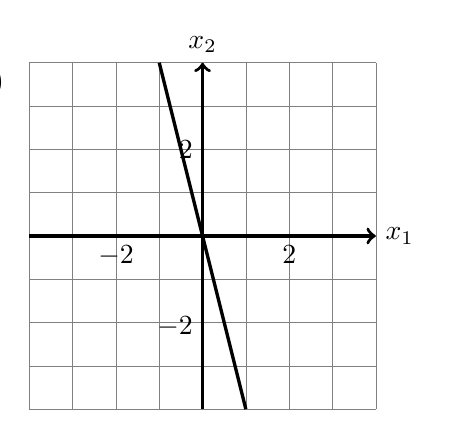
\begin{tikzpicture}[scale=.55]
    \draw[help lines] (-4, -4) grid (4, 4);
\draw[very thick, ->] (-4, 0) -- (4, 0);
\draw[very thick, ->] (0, -4) -- (0, 4);
\node[above] at (0, 4) {$x_2$};
\node[right] at (4, 0) {$x_1$};
\node[left] at (0, 2) {$2$};
\node[below] at (2, 0) {$2$};
\node[below] at (-2, 0) {$-2$};
\node[left] at (0, -2.1) {$-2$};    
    \node[overlay, above] at (-5, 3) {(a)};
    \draw[very thick, -] (1, -4) -- (-1, 4);    
    \end{tikzpicture}\qquad
    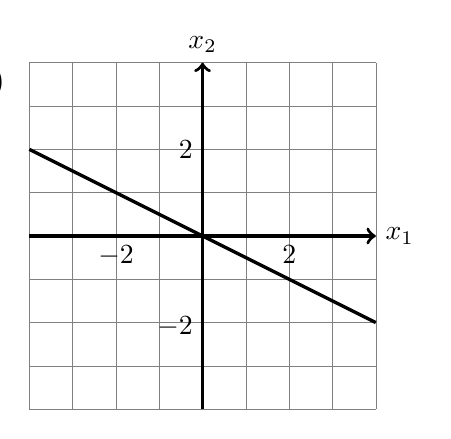
\begin{tikzpicture}[scale=.55]
    \draw[help lines] (-4, -4) grid (4, 4);
\draw[very thick, ->] (-4, 0) -- (4, 0);
\draw[very thick, ->] (0, -4) -- (0, 4);
\node[above] at (0, 4) {$x_2$};
\node[right] at (4, 0) {$x_1$};
\node[left] at (0, 2) {$2$};
\node[below] at (2, 0) {$2$};
\node[below] at (-2, 0) {$-2$};
\node[left] at (0, -2.1) {$-2$};    
    \node[overlay, above] at (-5, 3) {(b)};  
    \draw[very thick, -] (4, -2) -- (-4, 2);    
    \end{tikzpicture}
    \end{center}   }
   \else
    \vspace{-12pt}
    \begin{center}
    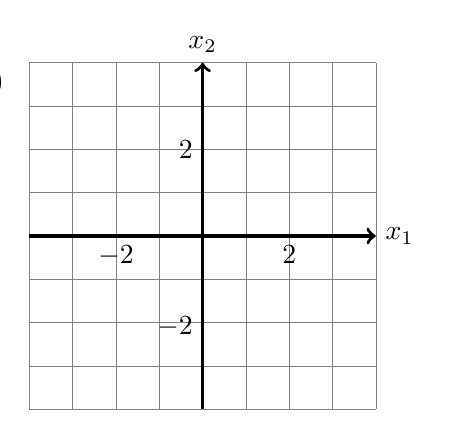
\begin{tikzpicture}[scale=.55]
    \draw[help lines] (-4, -4) grid (4, 4);
\draw[very thick, ->] (-4, 0) -- (4, 0);
\draw[very thick, ->] (0, -4) -- (0, 4);
\node[above] at (0, 4) {$x_2$};
\node[right] at (4, 0) {$x_1$};
\node[left] at (0, 2) {$2$};
\node[below] at (2, 0) {$2$};
\node[below] at (-2, 0) {$-2$};
\node[left] at (0, -2.1) {$-2$};    
    \node[overlay, above] at (-5, 3) {(a)};
    \end{tikzpicture}\qquad
    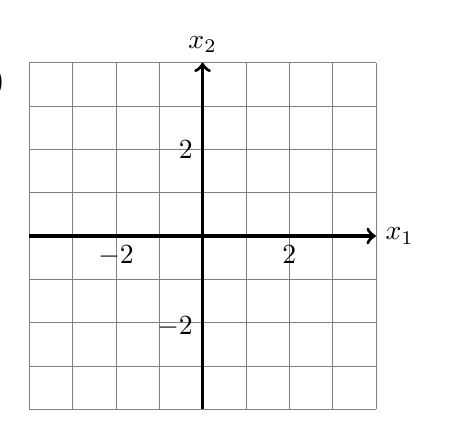
\begin{tikzpicture}[scale=.55]
    \draw[help lines] (-4, -4) grid (4, 4);
\draw[very thick, ->] (-4, 0) -- (4, 0);
\draw[very thick, ->] (0, -4) -- (0, 4);
\node[above] at (0, 4) {$x_2$};
\node[right] at (4, 0) {$x_1$};
\node[left] at (0, 2) {$2$};
\node[below] at (2, 0) {$2$};
\node[below] at (-2, 0) {$-2$};
\node[left] at (0, -2.1) {$-2$};    
    \node[overlay, above] at (-5, 3) {(b)};    
    \end{tikzpicture}
    \end{center}   
   \fi
\fi



\ifnum \Version = 11
\question[2] Construct an orthogonal basis for $W = \text{Span}\{v_1,v_2\}$. Please show your work. 
$$v_1 = \begin{pmatrix} 1\\1\\1\end{pmatrix}, \quad v_2 = \begin{pmatrix} 3\\5\\1\end{pmatrix}$$

\ifnum \Solutions=1 {\color{DarkBlue} \textit{Solutions.} Set $\hat v_1 = v_1$ and $\hat v_2$ to be
$$\hat v_2 = v_2 - \frac{v_1\cdot v_2}{v_1\cdot v_1} v_1 = \begin{pmatrix} 3\\5\\1\end{pmatrix} - \frac{9}{3}\begin{pmatrix} 1\\1\\1\end{pmatrix} = \begin{pmatrix} 0\\2\\-2\end{pmatrix}$$ An orthogonal basis is $$\left\{ \begin{pmatrix}1\\1\\1 \end{pmatrix}, \begin{pmatrix} 0\\2\\-2\end{pmatrix}\right\}$$
}
\fi
\fi


\ifnum \Version = 12
\question[2] Suppose $A = \begin{pmatrix} 2&1\\8&4 \end{pmatrix}$. On the grids below, sketch a) the range of the transform $x \to Ax$, and b) $(\Row A)^{\perp}$. You do not need to show your work. 

\ifnum \Solutions=1 {\color{DarkBlue} \textit{Solutions.} \begin{itemize}
    \item[a)] The range is the span of the columns of $A$, and a vector in the span of the columns is $\begin{pmatrix} 1 & 4\end{pmatrix}^T$. We can sketch a line that passes through the origin and the point $(1,4)$. Note also that the span is a line that is defined for any value of $x_1$. So to sketch the span correctly, the line needs to extend to the edges of the graph. 
    \item[b)] Remember that $(\Row A)^{\perp} = \Null A$. The rows are dependent, so we can ignore one of the rows and use the other to sketch the space. For example we can sketch the line that passes through the origin and the point $(2,-1)$. Note also that the span is a line that is defined for any value of $x_1$. So to sketch the span correctly, the line needs to extend to the edges of the graph. 
    \end{itemize}
    \vspace{-12pt}
    \begin{center}
    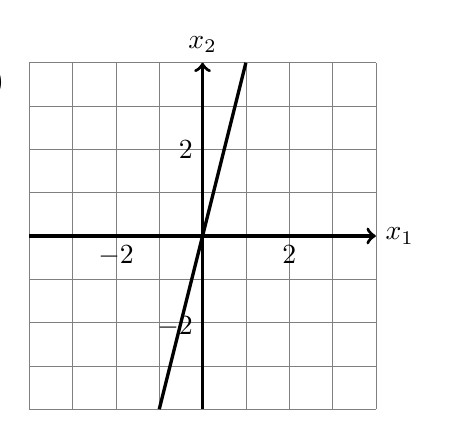
\begin{tikzpicture}[scale=.55]
    \draw[help lines] (-4, -4) grid (4, 4);
\draw[very thick, ->] (-4, 0) -- (4, 0);
\draw[very thick, ->] (0, -4) -- (0, 4);
\node[above] at (0, 4) {$x_2$};
\node[right] at (4, 0) {$x_1$};
\node[left] at (0, 2) {$2$};
\node[below] at (2, 0) {$2$};
\node[below] at (-2, 0) {$-2$};
\node[left] at (0, -2.1) {$-2$};    
    \node[overlay, above] at (-5, 3) {(a)};
    \draw[very thick, -] (-1,-4) -- (1,4);    
    \end{tikzpicture}\qquad
    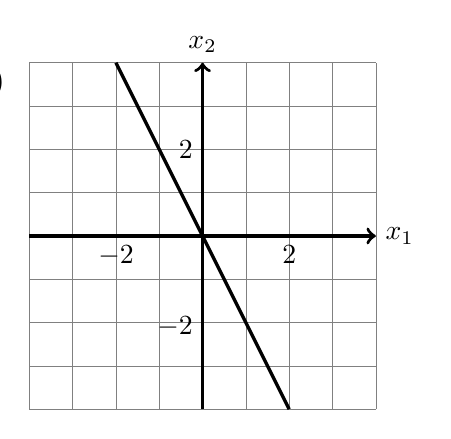
\begin{tikzpicture}[scale=.55]
    \draw[help lines] (-4, -4) grid (4, 4);
\draw[very thick, ->] (-4, 0) -- (4, 0);
\draw[very thick, ->] (0, -4) -- (0, 4);
\node[above] at (0, 4) {$x_2$};
\node[right] at (4, 0) {$x_1$};
\node[left] at (0, 2) {$2$};
\node[below] at (2, 0) {$2$};
\node[below] at (-2, 0) {$-2$};
\node[left] at (0, -2.1) {$-2$};    
    \node[overlay, above] at (-5, 3) {(b)};  
    \draw[very thick, -] (-2, 4) -- (2, -4);    
    \end{tikzpicture}
    \end{center}   }
   \else
    \vspace{-12pt}
    \begin{center}
    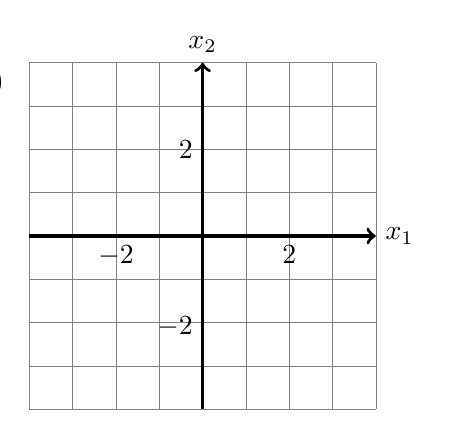
\begin{tikzpicture}[scale=.55]
    \draw[help lines] (-4, -4) grid (4, 4);
\draw[very thick, ->] (-4, 0) -- (4, 0);
\draw[very thick, ->] (0, -4) -- (0, 4);
\node[above] at (0, 4) {$x_2$};
\node[right] at (4, 0) {$x_1$};
\node[left] at (0, 2) {$2$};
\node[below] at (2, 0) {$2$};
\node[below] at (-2, 0) {$-2$};
\node[left] at (0, -2.1) {$-2$};    
    \node[overlay, above] at (-5, 3) {(a)};
    \end{tikzpicture}\qquad
    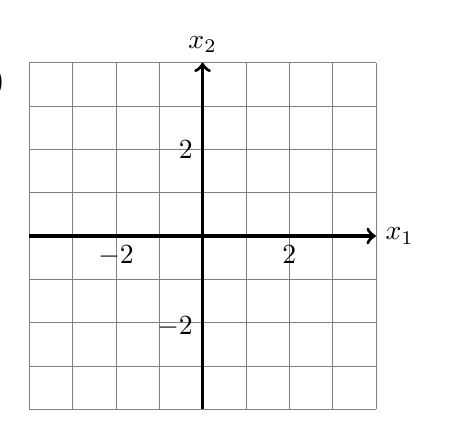
\begin{tikzpicture}[scale=.55]
    \draw[help lines] (-4, -4) grid (4, 4);
\draw[very thick, ->] (-4, 0) -- (4, 0);
\draw[very thick, ->] (0, -4) -- (0, 4);
\node[above] at (0, 4) {$x_2$};
\node[right] at (4, 0) {$x_1$};
\node[left] at (0, 2) {$2$};
\node[below] at (2, 0) {$2$};
\node[below] at (-2, 0) {$-2$};
\node[left] at (0, -2.1) {$-2$};    
    \node[overlay, above] at (-5, 3) {(b)};    
    \end{tikzpicture}
    \end{center}   
   \fi
\fi



\ifnum \Version = 13
\question[2] Suppose $A = \begin{pmatrix} 4&1\\8&2 \end{pmatrix}$. On the grids below, sketch a) the eigenspace corresponding to eigenvalue $\lambda = 6$, and b) $(\Null A)^{\perp}$. You do not need to show your work. 


\ifnum \Solutions=1 {\color{DarkBlue} \textit{Solutions.} \begin{itemize}
    \item[a)] The eigenspace is the space spanned by vectors in $\Null(A - \lambda I)$. $$A - \lambda I = \begin{pmatrix}-2&1\\8&-4 \end{pmatrix}$$ A vector in the nullspace is the eigenvector $v = \begin{pmatrix} 1\\2\end{pmatrix}$. We can sketch a line that passes through the origin and the point $(1,2)$. Note also that the span is a line that is defined for any value of $x_1$. So to sketch the span correctly, the line needs to extend to the edges of the graph. 
\item[b)] Remember that $(\Null A)^{\perp} = \Row A$. The rows are dependent, so we can ignore one of the rows and use the other to sketch the space. For example we can sketch the line that passes through the origin and the point $(4,1)$. Note also that the span is a line that is defined for any value of $x_1$. So to sketch the span correctly, the line needs to extend to the edges of the graph. 
\end{itemize}
    \vspace{-12pt}
    \begin{center}
    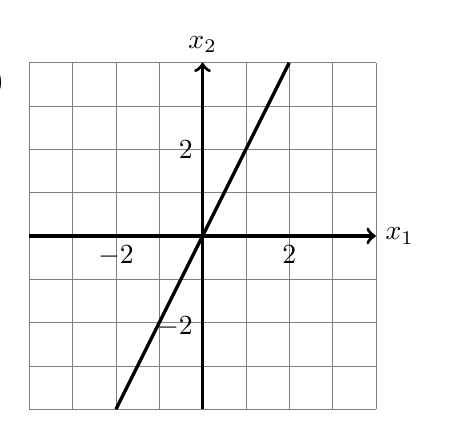
\begin{tikzpicture}[scale=.55]
    \draw[help lines] (-4, -4) grid (4, 4);
\draw[very thick, ->] (-4, 0) -- (4, 0);
\draw[very thick, ->] (0, -4) -- (0, 4);
\node[above] at (0, 4) {$x_2$};
\node[right] at (4, 0) {$x_1$};
\node[left] at (0, 2) {$2$};
\node[below] at (2, 0) {$2$};
\node[below] at (-2, 0) {$-2$};
\node[left] at (0, -2.1) {$-2$};    
    \node[overlay, above] at (-5, 3) {(a)};
    \draw[very thick, -] (-2,-4) -- (2,4);    
    \end{tikzpicture}\qquad
    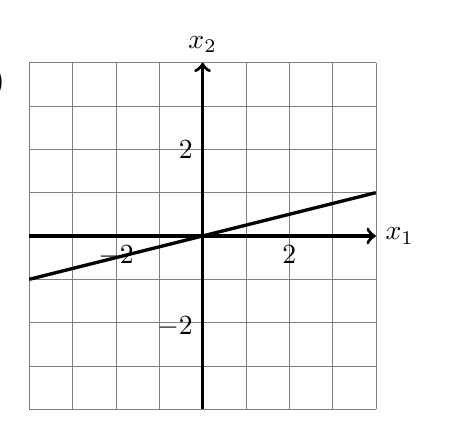
\begin{tikzpicture}[scale=.55]
    \draw[help lines] (-4, -4) grid (4, 4);
\draw[very thick, ->] (-4, 0) -- (4, 0);
\draw[very thick, ->] (0, -4) -- (0, 4);
\node[above] at (0, 4) {$x_2$};
\node[right] at (4, 0) {$x_1$};
\node[left] at (0, 2) {$2$};
\node[below] at (2, 0) {$2$};
\node[below] at (-2, 0) {$-2$};
\node[left] at (0, -2.1) {$-2$};    
    \node[overlay, above] at (-5, 3) {(b)};  
    \draw[very thick, -] (4, 1) -- (-4, -1);    
    \end{tikzpicture}
    \end{center}   }
   \else
    \vspace{-12pt}
    \begin{center}
    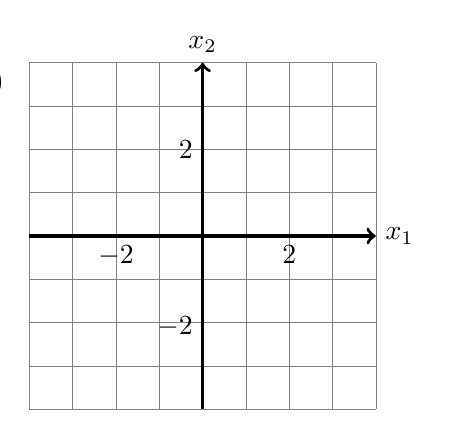
\begin{tikzpicture}[scale=.55]
    \draw[help lines] (-4, -4) grid (4, 4);
\draw[very thick, ->] (-4, 0) -- (4, 0);
\draw[very thick, ->] (0, -4) -- (0, 4);
\node[above] at (0, 4) {$x_2$};
\node[right] at (4, 0) {$x_1$};
\node[left] at (0, 2) {$2$};
\node[below] at (2, 0) {$2$};
\node[below] at (-2, 0) {$-2$};
\node[left] at (0, -2.1) {$-2$};    
    \node[overlay, above] at (-5, 3) {(a)};
    \end{tikzpicture}\qquad
    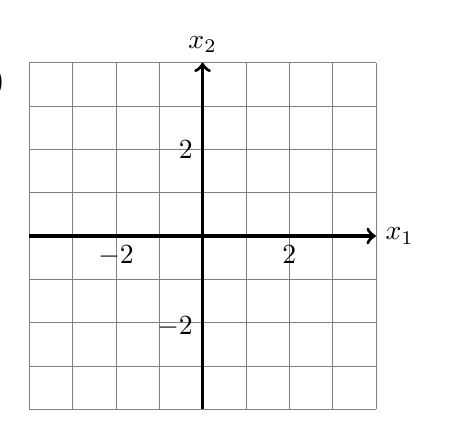
\begin{tikzpicture}[scale=.55]
    \draw[help lines] (-4, -4) grid (4, 4);
\draw[very thick, ->] (-4, 0) -- (4, 0);
\draw[very thick, ->] (0, -4) -- (0, 4);
\node[above] at (0, 4) {$x_2$};
\node[right] at (4, 0) {$x_1$};
\node[left] at (0, 2) {$2$};
\node[below] at (2, 0) {$2$};
\node[below] at (-2, 0) {$-2$};
\node[left] at (0, -2.1) {$-2$};    
    \node[overlay, above] at (-5, 3) {(b)};    
    \end{tikzpicture}
    \end{center}   
   \fi
\fi



\ifnum \Version = 20 %% NOT USING BUT COULD BE A GOOD QUESTION
\question[2] Construct an orthogonal basis for $W = \text{Span}\{v_1,v_2\}$. Please show your work. 
$$v_1 = \begin{pmatrix} 1\\1\\1\end{pmatrix}, \quad v_2 = \begin{pmatrix} 6\\10\\2\end{pmatrix}$$

\ifnum \Solutions=1 {\color{DarkBlue} \textit{Solutions.} NEED TO FIX THE SOLUTIONS THERE ARE SOME TYPOS HERE: Set $\hat v_1 = v_1$ and $\hat v_2$ to be
$$\hat v_2 = v_2 - \frac{v_1\cdot v_2}{v_1\cdot v_1} v_1 = \begin{pmatrix} 3\\5\\1\end{pmatrix} - \frac{18}{3}\begin{pmatrix} 1\\1\\1\end{pmatrix} = \begin{pmatrix} 3\\5\\1\end{pmatrix} -\begin{pmatrix} 6\\6\\6\end{pmatrix}= \begin{pmatrix}-3\\-1\\-5 \end{pmatrix}$$ An orthogonal basis is $$\left\{ \begin{pmatrix}1\\1\\1 \end{pmatrix}, \begin{pmatrix} 0\\2\\-2\end{pmatrix}\right\}$$
}
\fi
\fi % some versions have a 2-point question

\newpage
\question[0.25] \ID
\question[4]

\ifnum \Version=1 
    Consider the system of linear equations $Ax=b$, where $A$ and $b$ are given below. 
    \begin{align*}
        A = \begin{pmatrix} 1&0&1&-2\\2&0&3&-7\\1&0&3&-8\end{pmatrix}, \ b = \begin{pmatrix} 2\\5\\4 \end{pmatrix}
    \end{align*}
    \begin{parts}
        \part Express the system as a $3\times5$ augmented matrix, $\begin{pmatrix} A & b\end{pmatrix}$, and then reduce the augmented matrix to RREF. Please show your work. 
        \ifnum \Solutions=1 {\color{DarkBlue}
        \begin{align}
        \begin{pmatrix} A & b \end{pmatrix} 
        = \begin{pmatrix} 1&0&1&-2&2\\2&0&3&-7&5\\1&0&3&-8&4\end{pmatrix} 
        \sim \begin{pmatrix} 1&0&1&-2&2\\0&0&1&-3&1\\0&0&2&-6&2\end{pmatrix} 
        \sim \begin{pmatrix} 1&0&0&1 &1 \\0&0&1&-3&1\\0&0&0&0&0\end{pmatrix} 
        \end{align}
        
        } 
        \else
        \vspace{9cm}
        \fi
        \part Use your results in part (a) to state a basis for $\Col A$. You do not need to show your work.
        \ifnum \Solutions=1 {\color{DarkBlue} \\
        A basis for $\Col A$ is given by the pivotal columns of the original matrix (not the RREF). 
        $$\left\{ \begin{pmatrix} 1\\2\\1\end{pmatrix}, \begin{pmatrix} 1\\3\\3 \end{pmatrix}\right\}$$
        } 
        \else
        \vspace{2cm}
        \fi
        \part If possible, use your results in part (a) to express the solution set of the linear system $Ax=b$ in parametric vector form. You do not need to show your work.
        \ifnum \Solutions=1 {\color{DarkBlue}\\
        By inspection:
        \begin{align}
            \vec x = \begin{pmatrix}x_1\\x_2\\x_3\\x_4 \end{pmatrix} = \begin{pmatrix} 1-x_4\\x_2\\1 +3x_4 \\x_4\end{pmatrix} = \begin{pmatrix} 1\\0\\1\\0\end{pmatrix} + x_2 \begin{pmatrix} 0\\1\\0\\0 \end{pmatrix} + x_4\begin{pmatrix} -1\\0\\3\\1\end{pmatrix}
        \end{align}
        } 
        \fi        
    \end{parts}
\fi



\ifnum \Version=2
Consider the quadratic form $Q = \vec x ^T A \vec x = 5x_1^2 - 5x_2^2 + 5x_3^2 + 6x_1x_3$, where  $A = A^T$ and $\vec x = \begin{pmatrix} x_1 & x_2 & x_3 \end{pmatrix}^T$. The eigenvalues of the symmetric matrix $A$ are $\lambda_1 = 8$, $\lambda_2 = 2$, and $\lambda_3 = -5$. 

\begin{parts}
    \part Construct matrix $A$. For this part you can state the matrix, you do not need to show work for this part because it can be done by inspection. 
    
    \ifnum \Solutions=1 {\color{DarkBlue}
    The matrix is $$A = \begin{pmatrix} 5&0&3\\0&-5&0\\3&0&5\end{pmatrix}$$  
    } 
    \else 
    \vspace{3 cm}
    \fi    

    
    \part Determine all locations where $Q$ is maximized subject to the constraint that $\|\vec x \| = 1$.  Please show your work.
    
    \ifnum \Solutions=1 {\color{DarkBlue}
    The eigenvector corresponding to the largest eigenvalue is in the null space of 
    \begin{align}
        A - \lambda_1 I = \begin{pmatrix} 5&0&3\\0&-5&0\\3&0&5\end{pmatrix} - \begin{pmatrix} 8&0&0\\0&8&0\\0&0&8\end{pmatrix} = \begin{pmatrix} -3&0&3\\0&-13&0\\3&0&-3\end{pmatrix}
    \end{align}
    A vector in the null space is
    \begin{align}
        \vec v_1 = \begin{pmatrix} 1\\0\\1\end{pmatrix}
    \end{align}
    The maximum values of $Q$ are obtained at two locations: 
    \begin{align}
        \pm \frac{1}{\sqrt 2} \vec v_1 = \pm \frac{1}{\sqrt 2}  \begin{pmatrix} 1\\0\\1\end{pmatrix}
    \end{align}    
    } 
    \else 
    \vspace{7 cm}
    \fi    

    
    \part Determine all locations where $Q$ is minimized subject to the constraint that $\|\vec x \| = 1$. Please show your work.
    
    \ifnum \Solutions=1 {\color{DarkBlue}
    The eigenvector corresponding to the smallest eigenvalue is in the null space of 
        \begin{align}
            A - \lambda_3 I = \begin{pmatrix} 5&0&3\\0&-5&0\\3&0&5\end{pmatrix} + (-5) \begin{pmatrix} 1&0&0\\0&1&0\\0&0&1\end{pmatrix} = \begin{pmatrix} 10&0&3\\0&0&0\\3&0&10\end{pmatrix}
        \end{align}
        A vector in the null space is
        \begin{align}
            \vec v_3 = \begin{pmatrix} 0\\1\\0\end{pmatrix}
        \end{align}
        The minimum values of $Q$ are obtained at two locations: 
        \begin{align}
            \pm \vec v_3 = \pm \begin{pmatrix} 0 \\1\\0\end{pmatrix}
        \end{align}           
    } 
    \else 
    \vspace{2 cm}
    \fi    
\end{parts}
\fi



\ifnum \Version=3
    Consider the system of linear equations $Ax=b$, where $A$ and $b$ are given below. 
    \begin{align*}
        A = \begin{pmatrix} 1&1&0&-2\\2&3&0&-7\\1&3&0&-8\end{pmatrix}, \ b = \begin{pmatrix} 2\\5\\4 \end{pmatrix}
    \end{align*}
    \begin{parts}
        \part Express the system as a $3\times5$ augmented matrix, $\begin{pmatrix} A & b\end{pmatrix}$, and then reduce the augmented matrix to RREF. Please show your work. 
        \ifnum \Solutions=1 {\color{DarkBlue}
        \begin{align}
        \begin{pmatrix} A & b \end{pmatrix} 
        = \begin{pmatrix} 1&1&0&-2&2\\2&3&0&-7&5\\1&3&0&-8&4\end{pmatrix} 
        \sim \begin{pmatrix} 1&1&0&-2&2\\0&1&0&-3&1\\0&2&0&-6&2\end{pmatrix} 
        \sim \begin{pmatrix} 1&0&0&1 &1 \\0&1&0&-3&1\\0&0&0&0&0\end{pmatrix} 
        \end{align}
        
        } 
        \else
        \vspace{9cm}
        \fi
        \part Use your results in part (a) to state a basis for $\Col A$. You do not need to show your work.
        \ifnum \Solutions=1 {\color{DarkBlue} \\
        A basis for $\Col A$ is given by the pivotal columns of the original matrix (not the RREF). 
        $$\left\{ \begin{pmatrix} 1\\2\\1\end{pmatrix}, \begin{pmatrix} 1\\3\\3 \end{pmatrix}\right\}$$
        } 
        \else
        \vspace{2cm}
        \fi
        \part If possible, use your results in part (a) to express the solution set of the linear system $Ax=b$ in parametric vector form. You do not need to show your work.
        \ifnum \Solutions=1 {\color{DarkBlue}\\
        By inspection:
        \begin{align}
            \vec x = \begin{pmatrix}x_1\\x_2\\x_3\\x_4 \end{pmatrix} = \begin{pmatrix} 1-x_4\\1+3x_4\\x_3\\x_4\end{pmatrix} = \begin{pmatrix} 1\\1\\0\\0\end{pmatrix} + x_3 \begin{pmatrix} 0\\0\\1\\0 \end{pmatrix} + x_4\begin{pmatrix} -1\\3\\0\\1\end{pmatrix}
        \end{align}
        } 
        \fi        
    \end{parts}
\fi



\ifnum \Version=4
    Consider the matrix $
        A = \begin{pmatrix} 1&1\\1&0\\0&1 \end{pmatrix}$.
    \begin{parts}
    \part Calculate $A^TA$.
    \ifnum \Solutions=1 {\color{DarkBlue}
    $A^TA$ is
        \begin{align}
            A^TA = \begin{pmatrix} 1&1&0\\1&0&1 \end{pmatrix}\begin{pmatrix} 1&1\\1&0\\0&1 \end{pmatrix}= \begin{pmatrix} 2&1\\1&2\end{pmatrix}
        \end{align}
    } 
    \else 
    \vspace{2cm}
    \fi
    \part Determine the singular values of $A$. Please show your work. 
    \ifnum \Solutions=1 {\color{DarkBlue}
    The eigenvalues of $A^TA$ are $1$ and $3$ because $A-3I$ and $A-I$ are singular. The square roots of the eigenvalues are the singular values, so 
    $$\sigma_1 = \sqrt3, \sigma_2=1$$
    Note that the largest singular value must be the first singular value. It would not be correct to set $\sigma_2 = \sqrt3$. 
    } 
    \else 
    \vspace{5 cm}
    \fi
    \part Determine the first right singular vector of $A$, $\vec v_1$. Please show your work.
    \ifnum \Solutions=1 {\color{DarkBlue}
    The right singular vectors are the unit eigenvectors of $A^TA$. The first right singular vector is a unit eigenvector that corresponds to $\sigma_1$, which is the positive square root of the largest eigenvalue of $A^TA$. 
        \begin{align}
            A^TA  - \lambda_1 I = A^TA  - \sigma_1^2 I = \begin{pmatrix} 2&1\\1&2 \end{pmatrix} - 3\begin{pmatrix} 1&0\\0&1 \end{pmatrix} = \begin{pmatrix} -1&1\\1&-1 \end{pmatrix}
        \end{align}
        A unit vector in the null space of this matrix is the vector 
        \begin{align}
            \vec v_1 = \frac{1}{\sqrt 2}\begin{pmatrix} 1\\1\end{pmatrix}
        \end{align}
        It is ok to use the negative of this vector. 
        \begin{align}
            \vec v_1 = -\frac{1}{\sqrt 2}\begin{pmatrix} 1\\1\end{pmatrix}
        \end{align}
        But those two vectors are the only two possible answers for this part. 
    } 
    \else 
    \vspace{5 cm}
    \fi
    \part Determine the first left singular vector of $A$, $\vec u_1$. Please show your work.
    \ifnum \Solutions=1 {\color{DarkBlue}
    The first left singular vector can be found using the usual formula
        $$\vec u_1 = \frac{1}{\sigma_1} A\vec v_1$$
        Using our values for $\vec v_1$, $\sigma_1$ and $A$, we obtain
        \begin{align}
            \vec u_1 
            = \frac{1}{\sqrt3}\begin{pmatrix} 1&1\\1&0\\0&1\end{pmatrix} \begin{pmatrix} 1/\sqrt{2}\\1/\sqrt2\end{pmatrix} 
            = \frac{1}{\sqrt3} \begin{pmatrix} 2/\sqrt2\\1/\sqrt2\\1/\sqrt2\end{pmatrix} = \frac{1}{\sqrt6}\begin{pmatrix}2\\1\\1 \end{pmatrix}
        \end{align}
    } 
    
    \fi    
    \end{parts}
\fi 

\ifnum \Version=5
    Suppose $A = \begin{pmatrix} 4&-6\\3&8\\0&0 \end{pmatrix}$. 
\begin{parts}
    \part Calculate $A^TA$ and the singular values of $A$. Please show your work.
    
    \ifnum \Solutions=1 {\color{DarkBlue} \textit{Solutions.} 
    $A^TA$ is
        \begin{align}
            A^TA = \begin{pmatrix} 4&3&0\\-6&8&0 \end{pmatrix}\begin{pmatrix} 4&-6\\3&8\\0&0 \end{pmatrix}= \begin{pmatrix} 25&0\\0&100\end{pmatrix}
        \end{align}
        The eigenvalues of $A^TA$ are $\lambda_1 = 100$ and $\lambda_2 = 25$. So $\sigma_1 = 10$, and $\sigma_2 = 5$. 
    } 
   \else
      \vspace{5cm}
   \fi
    \part Determine the first right singular vector of $A$, $\vec v_1$. Please show your work.
    
    \ifnum \Solutions=1 {\color{DarkBlue} \textit{Solutions.} 

    The right singular vectors are the unit eigenvectors of $A^TA$. The first right singular vector is a unit eigenvector that corresponds to $\sigma_1$, which is the positive square root of the largest eigenvalue of $A^TA$. 
        \begin{align}
            A^TA  - \lambda_1 I = A^TA  - \sigma_1^2 I = \begin{pmatrix} 25&0\\0&100 \end{pmatrix} - \begin{pmatrix} 100&0\\0&100 \end{pmatrix} \sim \begin{pmatrix} 1&0\\0&0 \end{pmatrix}
        \end{align}
        A unit vector in the null space of this matrix is the vector 
        \begin{align}
            \vec v_1 = \begin{pmatrix} 0\\1\end{pmatrix}
        \end{align}
        It is ok to use the negative of this vector, the SVD is not unique. But $\vec v_1$ must have unit length. 
    } 
   \else
      \vspace{6cm}
   \fi    
    \part Determine the first left singular vector of $A$, $\vec u_1$. Please show your work.
    
    \ifnum \Solutions=1 {\color{DarkBlue} \textit{Solutions.} 
    The first left singular vector can be found using the usual formula
    $$\vec u_1 = \frac{1}{\sigma_1} A\vec v_1$$
    Using our values for $\vec v_1$, $\sigma_1$ and $A$, we obtain
    \begin{align}
        \vec u_1 = \frac{1}{10}\begin{pmatrix} 4&-6\\3&8\\0&0 \end{pmatrix} \begin{pmatrix} 0\\1 \end{pmatrix} = \frac{1}{10}\begin{pmatrix} -6\\8\\0 \end{pmatrix} 
    \end{align}
    }       
   \fi    
\end{parts}
\fi




\ifnum \Version=6
    Suppose $A = \begin{pmatrix} 1&0\\6&5 \end{pmatrix}$. 
    \begin{parts}
    \part Calculate the eigenvalues of $A$. 
    
    \ifnum \Solutions=1 {\color{DarkBlue} \textit{Solutions.} 
    $A$ is triangular, so the eigenvalues must be the entries on the main diagonal. We can set $\lambda_1 = 1$ and $\lambda_2 = 5$. 
    } 
   \else
      \vspace{3cm}
   \fi
    \part Determine the eigenvectors of $A$. 
    
    \ifnum \Solutions=1 {\color{DarkBlue} \textit{Solutions.} 
    $\lambda_1$: $$A-\lambda_1I = \begin{pmatrix} 0&0\\6&4\end{pmatrix}$$ A vector in the nullspace is $\vec v_1 = \begin{pmatrix} 2\\-3\end{pmatrix}$.

    $\lambda_2$: $$A-\lambda_2 I = \begin{pmatrix} -4&0\\6&0\end{pmatrix}$$ A vector in the nullspace is $\vec v_1 = \begin{pmatrix} 0\\1\end{pmatrix}$.
} 
   \else
      \vspace{7cm}
   \fi    
    \part If possible, construct real matrices $P$, $P^{-1}$, and $D$ such that $A = PDP^{-1}$, where $D$ is a diagonal matrix.
    
    \ifnum \Solutions=1 {\color{DarkBlue} \textit{Solutions.} 
    The columns of $P$ are the eigenvectors of $A$, so 
    $$P = \begin{pmatrix} 2&0\\-3&1 \end{pmatrix}$$
    The inverse can be computed using the formula for the inverse of a $2\times 2$ matrix
    $$P^{-1} = \frac12 \begin{pmatrix} 1&0\\3&2 \end{pmatrix}$$
    And the $D$ matrix is diagonal and its diagonal entries are the eigenvalues of $A$. 
    $$D = \begin{pmatrix} 1&0\\0&5 \end{pmatrix}$$
    Don't forget that the entries on the main diagonal of $D$ must correspond to the columns of $P$. 
    }       
   \fi    
\end{parts}
\fi
\ifnum \Version=7
    Consider the system of linear equations $Ax=b$, where $A$ and $b$ are given below. 
    \begin{align*}
        A = \begin{pmatrix} 4&0&3&5\\8&0&7&1\\12&0&11&-3\end{pmatrix}, \ b = \begin{pmatrix} -1\\7\\15 \end{pmatrix}
    \end{align*}
    \begin{parts}
        \part Express the system as a $3\times5$ augmented matrix, $\begin{pmatrix} A & b\end{pmatrix}$, and then reduce the augmented matrix to RREF. Please show your work. 
        \ifnum \Solutions=1 {\color{DarkBlue}
        \begin{align}
        \begin{pmatrix} 4&0&3&5&-1\\8&0&7&1&7\\12&0&11&-3&15\end{pmatrix} 
        \sim \begin{pmatrix} 4&0&3&5&-1\\0&0&1&-9&9\\0&0&2&-18&18\end{pmatrix} 
        &\sim \begin{pmatrix} 4&0&0&32&-28\\0&0&1&-9&9\\0&0&0&0&0\end{pmatrix} \\
        &\sim \begin{pmatrix} 1&0&0&8&-7\\0&0&1&-9&9\\0&0&0&0&0\end{pmatrix} 
        \end{align}
        } 
        \else
        \vspace{9cm}
        \fi
        \part Use your results in part (a) to state a basis for $\Col A$. You do not need to show your work.
        \ifnum \Solutions=1 {\color{DarkBlue} \\
        A basis for $\Col A$ is given by the pivotal columns of the original matrix (not the RREF). We can use these vectors for the basis:
        $$\left\{ \begin{pmatrix} 4\\8\\12\end{pmatrix}, \begin{pmatrix} 3\\7\\11 \end{pmatrix}\right\}$$ Other choices are ok too. Any two independent vectors that are in $\Col A$ should also be a basis.
        } 
        \else
        \vspace{2cm}
        \fi
        \part If possible, use your results in part (a) to express the solution set of the linear system $Ax=b$ in parametric vector form. You do not need to show your work.
        \ifnum \Solutions=1 {\color{DarkBlue}\\
        By inspection:
        \begin{align}
            \vec x = \begin{pmatrix}x_1\\x_2\\x_3\\x_4 \end{pmatrix} 
            = \begin{pmatrix} -7-8x_4\\x_2\\9+9x_4\\x_4\end{pmatrix} 
            = \begin{pmatrix} -7\\0\\9\\0\end{pmatrix} 
            + x_2 \begin{pmatrix} 0\\1\\0\\0 \end{pmatrix} 
            + x_4\begin{pmatrix} -8\\0\\9\\1\end{pmatrix}
        \end{align}
        } 
        \fi        
    \end{parts}
\fi

\ifnum \Version=8
    Three points in $\mathbb R^2$ with coordinates $(x,y)$ are $(-1,-1)$, $(0,7)$, $(1,3)$. Our goal is to obtain the coefficients $c_0, c_1$, so that the function, $y(x)$, that best fits the given points, where $y = c_0 + c_1x$. 
    \begin{enumerate}
    \item[a)] Use the given data to construct an inconsistent linear system of the form $A\vec x=\vec b$, where $\vec x = \begin{pmatrix} c_0 & c_1 \end{pmatrix}^T$. You do not need to show your work (it can be done by inspection). 
    \ifnum \Solutions=1 {\color{DarkBlue} \\[12pt] 
        The system is $A\vec x = \vec b$, where 
            \begin{align}
                A = \begin{pmatrix}1&-1\\1&0\\1&1 \end{pmatrix}, 
                \quad \vec x = \begin{pmatrix} c_0\\c_1 \end{pmatrix},
                \quad \vec b = \begin{pmatrix} -1\\7\\3\end{pmatrix}
            \end{align}
            The ordering of the entries of $x$ is specified in the question and determines the columns of $A$. In other words the first column of $A$ must be the column of 1's. 
        } 
        \else 
        \vfill
        \fi
    \item[b)] Use your results from the previous items to construct the normal equations, that when solved, yield the coefficients $c_0$ and $c_1$. Express the equations as an augmented matrix with two rows. Do not solve your equations. 
    \ifnum \Solutions=1 {\color{DarkBlue} \\[12pt] 
    The normal equations are $A^TA\vec x = A^T\vec b$, with
    $$A^TA = \begin{pmatrix} 3&0\\0&2\end{pmatrix}, \quad A^T\vec b = \begin{pmatrix}9\\4\end{pmatrix}$$
    The augmented matrix is
    \begin{align}
        \begin{pmatrix} A^TA & A^T\vec b \end{pmatrix} 
        = \begin{pmatrix} 3&0&9\\0&2&4\end{pmatrix}
    \end{align}
    } 
    \else 
    \vfill
    \fi
    \item[c)] Use the normal equations and row operations to obtain the solution to the normal equations by reducing your augmented matrix to RREF. 
    \ifnum \Solutions=1 {\color{DarkBlue} \\[12pt] 
    Reducing to RREF yields 
    $$\begin{pmatrix} 1&0&3\\0&1&2\end{pmatrix}$$
    } 
    \else 
    \vspace{3cm}
    \fi
    \item[d)] Use the values you found for the coefficients to express $y$ in the form $y = c_0 + c_1x$. 
    \ifnum \Solutions=1 {\color{DarkBlue} \\[12pt] 
    $$y = 3 + 2x$$
    } 
    \else 
    \vspace{3cm}
    \fi
\end{enumerate}
\fi 


\ifnum \Version=9
    Consider the matrix below. 
    \begin{align}
        A = \begin{pmatrix} 4&4\\0&2\\2&0 \end{pmatrix}
    \end{align}
    The singular values of $A$ are $\sigma_1=6$ and $\sigma_2=2$.
    \begin{parts}
        \part Calculate $A^TA$. 
        \ifnum \Solutions=1 {\color{DarkBlue} \\[12pt] 
        The product $A^TA$ is
        \begin{align}
            A^TA = \begin{pmatrix} 4&0&2\\4&2&0 \end{pmatrix}\begin{pmatrix} 4&4\\0&2\\2&0 \end{pmatrix}= \begin{pmatrix} 20&16\\16&20\end{pmatrix}
        \end{align}
        } 
        \else 
        \vspace{3cm}
        \fi
        \part Determine the first right singular vector of $A$, $\vec v_1$. Please show your work.
        \ifnum \Solutions=1 {\color{DarkBlue} \\[12pt] 
        The right singular vectors are the unit eigenvectors of $A^TA$. The first right singular vector is a unit eigenvector that corresponds to $\sigma_1$, which is the positive square root of the largest eigenvalue of $A^TA$. 
        \begin{align}
            A^TA  - \lambda_1 I = A^TA  - \sigma_1^2 I = \begin{pmatrix} 20&16\\16&20 \end{pmatrix} - \begin{pmatrix} 36&0\\0&36 \end{pmatrix} = 16 \begin{pmatrix} -1&1\\1&-1 \end{pmatrix}
        \end{align}
        A unit vector in the null space of this matrix is the vector 
        \begin{align}
            \vec v_1 = \frac{1}{\sqrt 2}\begin{pmatrix} 1\\1\end{pmatrix}
        \end{align}
        It is ok to use the negative of this vector:
        \begin{align}
            -\frac{1}{\sqrt 2}\begin{pmatrix} 1\\1\end{pmatrix}
        \end{align}
        Note that the SVD is not unique. 
        } 
        \else 
        \vfill
        \fi
        \part Determine the first left singular vectors of $A$, $\vec u_1$. Please show your work.
        \ifnum \Solutions=1 {\color{DarkBlue} \\[12pt] 
        The first left singular vector can be found using the usual formula
        $$\vec u_1 = \frac{1}{\sigma_1} A\vec v_1$$
        Using our values for $\vec v_1$, $\sigma_1$ and $A$, we obtain
        \begin{align}
            \vec u_1 = \frac{1}{6}\begin{pmatrix} 4&4\\0&2\\2&0 \end{pmatrix} \begin{pmatrix} 1/\sqrt{2}\\1/\sqrt2\end{pmatrix} = \frac16 \begin{pmatrix} 8/\sqrt2\\2/\sqrt2\\2/\sqrt2\end{pmatrix} = \frac{1}{3\sqrt2}\begin{pmatrix}4\\1\\1 \end{pmatrix}
        \end{align}
        } 
        \else 
        \vfill
        \fi
    \end{parts}
\fi 
\ifnum \Version=10
    Suppose $A = \begin{pmatrix} 4&2\\2&1 \end{pmatrix}$. 
    \begin{parts}
    \part Calculate the eigenvalues of $A$. 
    
    \ifnum \Solutions=1 {\color{DarkBlue} \textit{Solutions.} 
    It isn't necessary to use the characteristic poly here. $A$ is singular, so we can tell by inspection that one eigenvalue is zero. And the other eigenvalue will have to be the trace of the matrix, which is $4+1 = 5$. 
    } 
   \else
      \vspace{3cm}
   \fi
    \part Determine the eigenvectors of $A$. 
    
    \ifnum \Solutions=1 {\color{DarkBlue} \textit{Solutions.} 
    $\lambda_1 = 0 $: $$A-\lambda_1I = A$$ A vector in the nullspace is $\vec v_1 = \begin{pmatrix} 1\\-2\end{pmatrix}$.

    $\lambda_2 = 5$: $$A-\lambda_2 I = \begin{pmatrix} -1&2\\2&1\end{pmatrix}$$ A vector in the nullspace is $\vec v_1 = \begin{pmatrix} 2\\1\end{pmatrix}$.
} 
   \else
      \vspace{7cm}
   \fi    
    \part If possible, construct real matrices $P$, and $D$ such that $A = PDP^{T}$, where $D$ is a diagonal matrix and $P$ is an orthogonal matrix.
    
    \ifnum \Solutions=1 {\color{DarkBlue} \textit{Solutions.} 
    The columns of $P$ are the unit eigenvectors of $A$, so 
    $$P = \frac{1}{\sqrt5} \begin{pmatrix} 1&2\\-2&1 \end{pmatrix}$$
    And the $D$ matrix is diagonal and its diagonal entries are the eigenvalues of $A$. 
    $$D = \begin{pmatrix} 0&0\\0&5 \end{pmatrix}$$
    Don't forget that the entries on the main diagonal of $D$ must correspond to the columns of $P$. And that because we need $P$ to be orthogonal that its columns need to have unit length. 
    }       
   \fi    
   \end{parts}
\fi 

\ifnum \Version=11
        Consider the system of linear equations $Ax=b$, where $A$ and $b$ are given below. 
    \begin{align*}
        A = \begin{pmatrix} 1&0&3&-2\\3&0&10&-8\\2&0&7&-6\end{pmatrix}, \ b = \begin{pmatrix} 4\\13\\9 \end{pmatrix}
    \end{align*}
    \begin{parts}
        \part Express the system as a $3\times5$ augmented matrix, $\begin{pmatrix} A & b\end{pmatrix}$, and then reduce the augmented matrix to RREF. Please show your work. 
        \ifnum \Solutions=1 {\color{DarkBlue}
        \begin{align}
        \begin{pmatrix} A & b \end{pmatrix} 
        = \begin{pmatrix} 1&0&3&-2&4\\3&0&10&-8&13\\2&0&7&-6&9\end{pmatrix} 
        \sim \begin{pmatrix} 1&0&3&-2&4\\0&0&1&-2&1\\0&0&1&-2&1\end{pmatrix} 
        \sim \begin{pmatrix} 1&0&0&4 &1 \\0&0&1&-2&1\\0&0&0&0&0\end{pmatrix} 
        \end{align}
        
        } 
        \else
        \vspace{9cm}
        \fi
        \part Use your results in part (a) to state a basis for $\Col A$. You do not need to show your work.
        \ifnum \Solutions=1 {\color{DarkBlue} \\
        A basis for $\Col A$ is given by the pivotal columns of the original matrix (not the RREF). 
        $$\left\{ \begin{pmatrix} 1\\3\\2\end{pmatrix}, \begin{pmatrix} 3\\10\\7 \end{pmatrix}\right\}$$
        } 
        \else
        \vspace{2cm}
        \fi
        \part If possible, use your results in part (a) to express the solution set of the linear system $Ax=b$ in parametric vector form. You do not need to show your work.
        \ifnum \Solutions=1 {\color{DarkBlue}\\
        By inspection:
        \begin{align}
            \vec x = \begin{pmatrix}x_1\\x_2\\x_3\\x_4 \end{pmatrix} 
            = \begin{pmatrix} 1-4x_4\\x_2\\1 + 2x_4 \\x_4\end{pmatrix} 
            = \begin{pmatrix} 1\\0\\1\\0\end{pmatrix} 
            + x_2 \begin{pmatrix} 0\\1\\0\\0 \end{pmatrix} 
            + x_4\begin{pmatrix} -4\\0\\2\\1\end{pmatrix}
        \end{align}
        } 
        \fi        
    \end{parts}
\fi 

\ifnum \Version=12
    Consider the quadratic form $Q = \vec x ^T A \vec x = 6x_1^2 - 4x_2^2 + 6x_3^2 + 6x_1x_3$, where $\vec x = \begin{pmatrix} x_1 & x_2 & x_3 \end{pmatrix}^T$, and $A = A^T$. The eigenvalues of symmetric matrix $A$ are $\lambda_1 = 9$, $\lambda_2 = 3$, and $\lambda_3 = -4$. 
    \begin{parts}
        \part Construct matrix $A$. For this part you can state the matrix, you do not need to show work for this part because it can be done by inspection. 
        \ifnum \Solutions=1 {\color{DarkBlue} \\[12pt] 
            The matrix is $$A = \begin{pmatrix} 6&0&3\\0&-4&0\\3&0&6\end{pmatrix}$$
        } 
        \else 
        \vspace{3cm}
        \fi
        \part Determine the locations where $Q$ is maximized subject to the constraint that $\|\vec x \| = 1$.
        \ifnum \Solutions=1 {\color{DarkBlue} \\[12pt] 
        The eigenvector corresponding to the largest eigenvalue is in the null space of 
        \begin{align}
            A - \lambda_1 I = \begin{pmatrix} 6&0&3\\0&-4&0\\3&0&6\end{pmatrix} - \begin{pmatrix} 9&0&0\\0&9&0\\0&0&9\end{pmatrix} = \begin{pmatrix} -3&0&3\\0&-13&0\\3&0&-3\end{pmatrix}
        \end{align}
        A vector in the null space is
        \begin{align}
            \vec v_1 = \begin{pmatrix} 1\\0\\1\end{pmatrix}
        \end{align}
        The maximum values of $Q$ are obtained at two locations: 
        \begin{align}
            \pm \frac{1}{\sqrt 2} \vec v_1 = \pm \frac{1}{\sqrt 2}  \begin{pmatrix} 1\\0\\1\end{pmatrix}
        \end{align}
        } 
        \else 
        \vfill
        \fi        
        \part Determine the locations where $Q$ is minimized subject to the constraint that $\|\vec x \| = 1$.
        \ifnum \Solutions=1 {\color{DarkBlue} \\[12pt] 
        The eigenvector corresponding to the smallest eigenvalue is in the null space of 
        \begin{align}
            A - \lambda_3 I = \begin{pmatrix} 6&0&3\\0&-4&0\\3&0&6\end{pmatrix} + \begin{pmatrix} 4&0&0\\0&4&0\\0&0&4\end{pmatrix} = \begin{pmatrix} 10&0&3\\0&0&0\\3&0&10\end{pmatrix}
        \end{align}
        A vector in the null space is
        \begin{align}
            \vec v_3 = \begin{pmatrix} 0\\1\\0\end{pmatrix}
        \end{align}
        The minimum values of $Q$ are obtained at two locations: 
        \begin{align}
            \pm \vec v_3 = \pm \begin{pmatrix} 0 \\1\\0\end{pmatrix}
        \end{align}     
        } 
        \else 
        \vfill
        \fi        
        \end{parts}
\fi 
\ifnum \Version=13 % 
    Consider the quadratic form
    $
        Q = \vec x ^T A \vec x = 6x_1^2 - 4x_2^2 + 6x_3^2 + 6x_1x_3
    $
    where $A = A^T$ and $\vec x = \begin{pmatrix} x_1 & x_2 & x_3 \end{pmatrix}^T$.
    The eigenvalues of symmetric matrix $A$ are $\lambda_1 = 9$, $\lambda_2 = 3$, and $\lambda_3 = -4$. 

\begin{parts}
    \part Construct matrix $A$. For this part you can state the matrix, you do not need to show work for this part because it can be done by inspection. \vspace{3cm}
    \part Determine all locations where $Q$ is maximized subject to the constraint $\|\vec x \| = 1$. Show your work. \vfill
    \part Determine all locations where $Q$ is minimized subject to the constraint $\|\vec x \| = 1$. Show your work.\vfill
\end{parts}
    \ifnum \Solutions=1 {\color{DarkBlue} \textit{Solution:} SOLUTION HERE  } \fi    
\fi 
\ifnum \Version=14 % 
    Suppose $A = \begin{pmatrix} 4&2\\3&3 \end{pmatrix}$. 
    \begin{parts}
    \part Calculate the eigenvalues of $A$.  Please show your work.
    
    \ifnum \Solutions=1 {\color{DarkBlue} \textit{Solutions.} 
    We can rely on the characteristic polynomial: $$\det(A- \lambda I) = (4-\lambda)(3 - \lambda) - 6 = \lambda^2 - 7 \lambda - 6 = (\lambda -1)(\lambda - 6)$$ Thus the eigenvalues can be $\lambda_1 = 1$ and $\lambda_2 = 6$. 
    } 
   \else
      \vspace{4cm}
   \fi
    \part Determine the eigenvectors of $A$. Please show your work.
    
    \ifnum \Solutions=1 {\color{DarkBlue} \textit{Solutions.} 
    $\lambda_1 = 1$: $$A-\lambda_1I = \begin{pmatrix} 3&2\\3&2\end{pmatrix}$$ A vector in the nullspace is $\vec v_1 = \begin{pmatrix} 2\\-3\end{pmatrix}$.

    $\lambda_2 = 6$: $$A-\lambda_2 I = \begin{pmatrix} -2&2\\3&-3\end{pmatrix}$$ A vector in the nullspace is $\vec v_1 = \begin{pmatrix} 1\\1\end{pmatrix}$.
} 
   \else
      \vspace{8cm}
   \fi    
    \part If possible, construct real matrices $P$, $P^{-1}$, and $D$ such that $A = PDP^{-1}$, where $D$ is a diagonal matrix.
    
    \ifnum \Solutions=1 {\color{DarkBlue} \textit{Solutions.} 
    The columns of $P$ are the eigenvectors of $A$, so 
    $$P = \begin{pmatrix} 2&1\\-3&1 \end{pmatrix}$$
    The inverse can be computed using the formula for the inverse of a $2\times 2$ matrix
    $$P^{-1} = \frac15 \begin{pmatrix} 1&-1\\3&2 \end{pmatrix}$$
    And the $D$ matrix is diagonal and its diagonal entries are the eigenvalues of $A$. 
    $$D = \begin{pmatrix} 1&0\\0&6 \end{pmatrix}$$
    Don't forget that the entries on the main diagonal of $D$ must correspond to the columns of $P$. 
    }       
   \fi    
\end{parts}
\fi 


\ifnum \Version=15 % shouldn't need this version for fall 2023
    OPEN RESPONSE ON UNIT 4 or UNIT 5 (eg - Gram Schmidt, SVD, Symmetric matrices, Least Squares, etc)
    \ifnum \Solutions=1 {\color{DarkBlue} \textit{Solution:} SOLUTION HERE  } \fi    
\fi 
\ifnum \Version=16 % shouldn't need this version for fall 2023
    OPEN RESPONSE ON UNIT 1, UNIT 2, OR UNIT 3 (eg - BASIS FOR A SUBSPACE, DIAGONALIZE A MATRIX, LU FACTORIZATION, INVERSE OF A 3x3, etc)
    \ifnum \Solutions=1 {\color{DarkBlue} \textit{Solution:} SOLUTION HERE  } \fi    
\fi 
\ifnum \Version=17 % shouldn't need this version for fall 2023
    OPEN RESPONSE ON UNIT 4 or UNIT 5 (eg - Gram Schmidt, SVD, Symmetric matrices, Least Squares, etc)
    \ifnum \Solutions=1 {\color{DarkBlue} \textit{Solution:} SOLUTION HERE  } \fi    
\fi 
\ifnum \Version=18 % shouldn't need this version for fall 2023
    OPEN RESPONSE ON UNIT 1, UNIT 2, OR UNIT 3 (eg - BASIS FOR A SUBSPACE, DIAGONALIZE A MATRIX, LU FACTORIZATION, INVERSE OF A 3x3, etc)
    \ifnum \Solutions=1 {\color{DarkBlue} \textit{Solution:} SOLUTION HERE  } \fi    
\fi 
\ifnum \Version=19 % shouldn't need this version for fall 2023
    OPEN RESPONSE ON UNIT 4 or UNIT 5 (eg - Gram Schmidt, SVD, Symmetric matrices, Least Squares, etc)
    \ifnum \Solutions=1 {\color{DarkBlue} \textit{Solution:} SOLUTION HERE  } \fi    
\fi 


\end{questions}

\end{document}